\documentclass[a4paper, 14pt]{extarticle}
\usepackage[margin=1in]{geometry}
\usepackage{amsfonts, amsmath, amssymb, amsthm}
\usepackage[none]{hyphenat}
\usepackage{fancyhdr} %create a custom header and footer
\usepackage[utf8]{inputenc}
\usepackage[english, main=ukrainian]{babel}
\usepackage{pgfplots}
\usepgfplotslibrary{fillbetween}
\usepackage{tikz}
\usepackage{graphicx}
\usepackage{caption}
\usepackage{float}
\usepackage{physics}
\usepackage[unicode]{hyperref}
\usepgfplotslibrary{polar}
\usepackage{ifthen}
\usetikzlibrary{spy}
\usetikzlibrary{intersections}
\usepackage{bbm}
\usetikzlibrary{spy, quotes, angles}


\fancyhead{}
\fancyfoot{}
\parindent 0ex
\DeclareMathOperator*\uplim{\overline{lim}}
\DeclareMathOperator*\downlim{\underline{lim}}
\def\stackbelow#1#2{\underset{\displaystyle\overset{\displaystyle\shortparallel}{#2}}{#1}}
\def\huge{\displaystyle}
\def\bigline{\vspace{5mm}\\}
\def\rightproof{$\boxed{\Rightarrow}$ }
\def\leftproof{$\boxed{\Leftarrow}$ }

\def\defin#1{\textbf{Definition {#1}}}
\def\ex#1{\textbf{Example {#1}}}
\def\rm#1{\textbf{Remark {#1}}}
\def\prp#1{\textbf{Proposition {#1}}}
\def\lm#1{\textbf{Lemma {#1}}}
\def\th#1{\textbf{Theorem {#1}}}
\def\crl#1{\textbf{Corollary {#1}}}
\def\proof{\textbf{Proof.}\\}
\def\proofMI{\textbf{Proof MI.}\\}
\def\contra{\textbf{!Proof.}\\}

\usepackage{pdfpages}

\newcommand{\sequence}[2][{}]{%
\ifthenelse{\equal{#1}{}}{$\{{#2}, n \geq 1 \}$}
{$\huge \left\{ {#2} = {#1}, n \geq 1 \right\}$}%
}

\newtheoremstyle{theoremdd}% name of the style to be used
  {\topsep}% measure of space to leave above the theorem. E.g.: 3pt
  {\topsep}% measure of space to leave below the theorem. E.g.: 3pt
  {\normalfont}% name of font to use in the body of the theorem
  {0pt}% measure of space to indent
  {\bfseries}% name of head font
  {}% punctuation between head and body
  { }% space after theorem head; " " = normal interword space
  {\thmname{#1}\thmnumber{ #2}\textnormal{\thmnote{ \textbf{#3}\\}}}

\theoremstyle{theoremdd}
\newtheorem{theorem}{Theorem}[subsection]
  
\theoremstyle{theoremdd}
\newtheorem{definition}[theorem]{Definition}

\theoremstyle{theoremdd}
\newtheorem{samedef}[theorem]{Definition}

\theoremstyle{theoremdd}
\newtheorem{example}[theorem]{Example}

\theoremstyle{theoremdd}
\newtheorem{proposition}[theorem]{Proposition}

\theoremstyle{theoremdd}
\newtheorem{remark}[theorem]{Remark}

\theoremstyle{theoremdd}
\newtheorem{lemma}[theorem]{Lemma}

\theoremstyle{theoremdd}
\newtheorem{corollary}[theorem]{Corollary}

\newenvironment{pf}{\vspace*{-3mm} \textbf{Proof. \\}}{$\blacksquare$}
\newenvironment{pfMI}{\vspace*{-3mm} \textbf{Proof MI. \\}}{$\blacksquare$}
\newenvironment{pfNoTh}{\textbf{Proof. \\}}{$\blacksquare$}
\def\departial#1#2{\dfrac{\partial {#1}}{\partial {#2}}}

%delete
\def\subsequence#1{$\displaystyle \left\{ {#1}, k\geq1 \right\}$}
\def\limitdef#1#2#3#4#5{$\displaystyle \forall #1 > 0: \exists #2(#1): \forall #3 \geq #2: \left|#4 - #5\right| < #1$}
\def\bounded#1#2#3{$\exists #1>0: \forall #2\geq1: \abs{#3} < #1$}

\def\proof{\textbf{Proof.}\\}
\def\qed{$\blacksquare$}

\addto\captionsukrainian{% Replace "english" with the language you use
  \renewcommand{\contentsname}%
    {Контент}%
}

\begin{document}

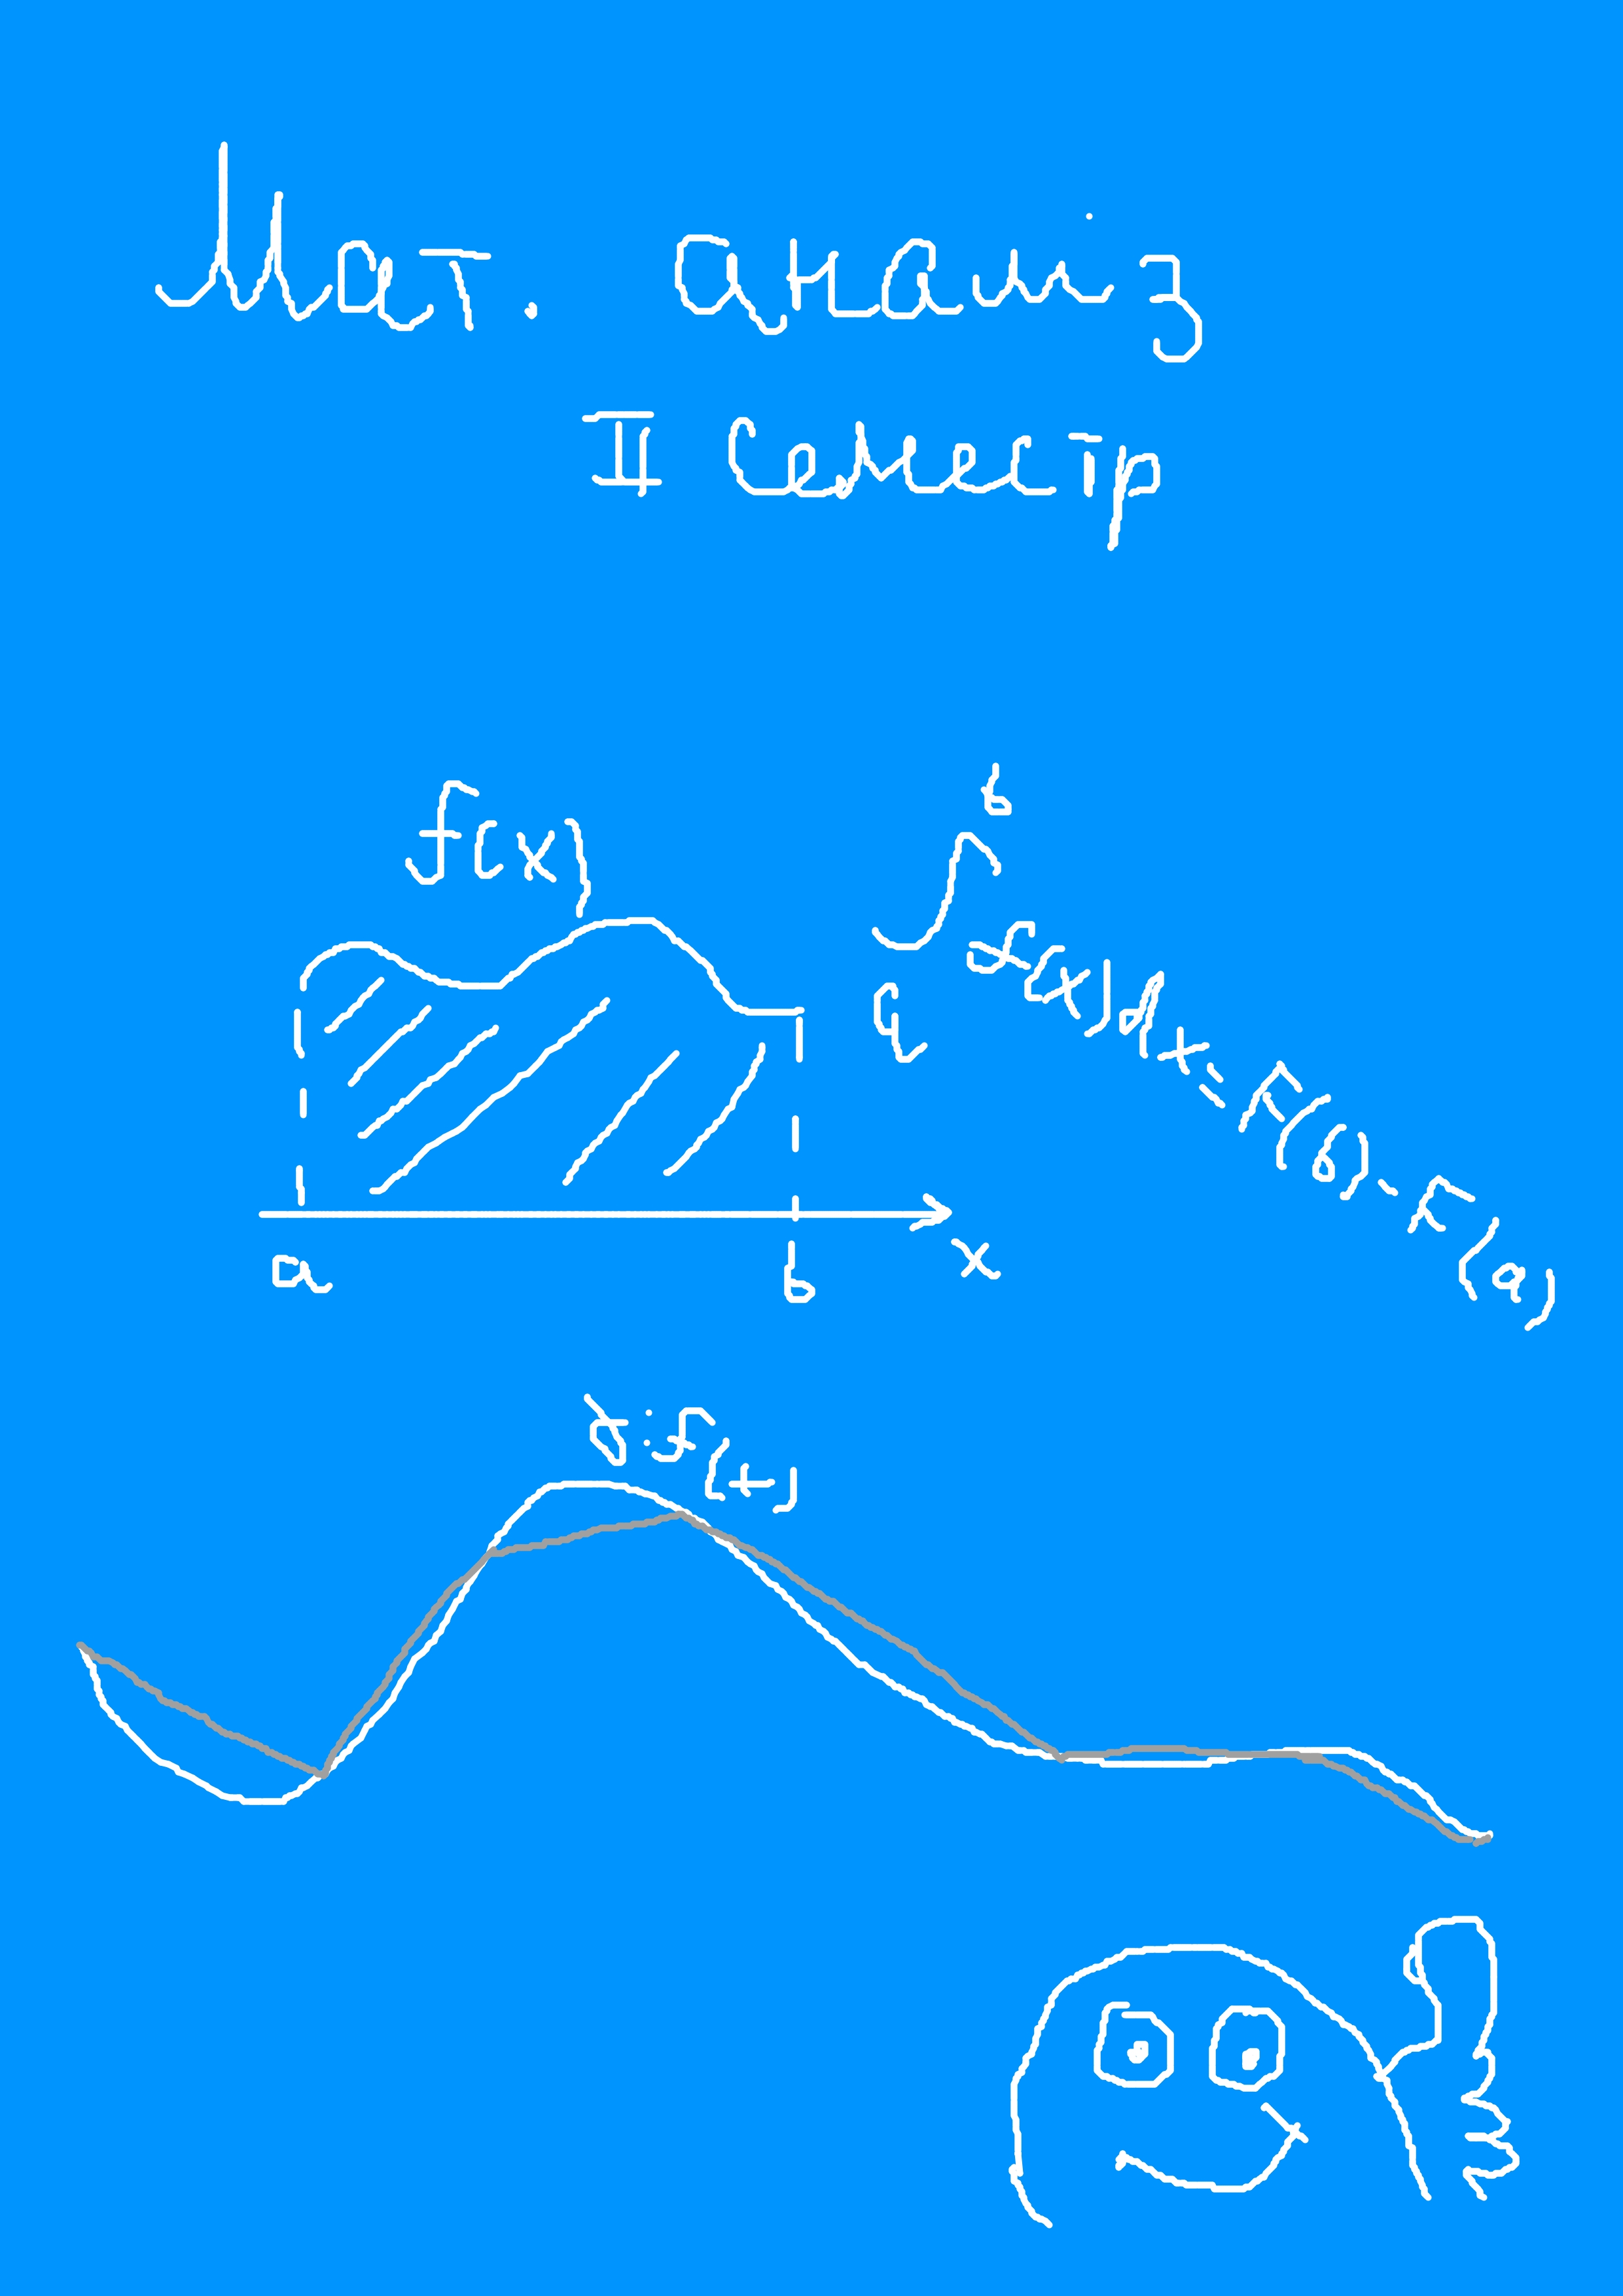
\includepdf{preview.jpg}

\tableofcontents
\newpage

\section*{Коротка передмова}
Дякую, що ти вижив на 1 семестрі. Це - матан в стилі Г.Б. Подколзіна
\bigline
Матеріал Г.Б. підбирав спеціально для студентів КН ММСА. Тому якщо комусь це попадеться в руки із СА/СП, май на увазі, що тут можуть бути не всі відомства або доведення деяких теорем можуть відрізнятися.
\bigline
Цей конспект писав студент. Тому в разі виявлення помилки - пишіть
\newpage

\section*{Авторські позначення}
\textbf{Definition} - означення\\
\textbf{Remark} - зауваження\\
\textbf{Theorem} - теорема\\
\textbf{Corollary} - наслідок\\
\textbf{Proposition} - твердження\\
\textbf{Lemma} - лема\\
\textbf{Example} - приклад
\bigline
\textbf{Proof} - доведення\\
Якщо будете бачити в шматочку доведення ! *якийсь текст* !, то це доведення якогось твердження від супротивного
\bigline
$C_{unif}$ - множина рівномірно неперервних функцій\\
$C^1, C^2, \dots$ - множина неперервних та диференційованих один раз, двічі, $\dots$ функцій

\newpage

\section*{Грубий лінал}
\subsection*{Про скалярний добуток}
Барановська давала позначення скалярного добутку через крапку: $\vec{a} \cdot \vec{b}$\\
Погана звичка: така нотація використовується для елементарних задач. А коли справа йде до узагальнення, то таке позначення призводить до плутанини\\
Віднині звикайте скалярний добуток писати в круглих дужках: $(\vec{a}, \vec{b})$

\subsection*{Про матриці}
Задано матрицю $B \in Mat(n \times n)$
\begin{definition}
Матрицю $B$ назвемо \textbf{симетричною}, якщо
\begin{align*}
B = B^T
\end{align*}
\end{definition}

\begin{definition}
Симетричну матрицю називають:\\
\textbf{строго додатньо визначеною}, якщо $\forall \vec{b} \in \mathbb{R}^n: (B \vec{b}, \vec{b}) > 0$\\
\textbf{строго від'ємно визначеною}, якщо $\forall \vec{b} \in \mathbb{R}^n: (B \vec{b}, \vec{b}) < 0$\\
\textbf{нестрого}, коли знаки нерівності будуть нестрогими
\bigline
А якщо $\exists \vec{b}_1, \vec{b_2} \in \mathbb{R}^n: (B\vec{b}_1, \vec{b}_1) < 0$ та $(B\vec{b}_2, \vec{b}_2) > 0$, то матриця називається \textbf{знако-невизначеною}
\end{definition}

\begin{definition}
\textbf{Головними кутовими мінорами} матриці $B = \begin{pmatrix}
b_{11} & \dots & b_{1n} \\
\vdots & \ddots & \vdots \\
b_{n1} & \dots & b_{nn}
\end{pmatrix}$ називають такі детермінанти 
\begin{align*}
\Delta_1 = \det (b_{11}) \hspace{0.5cm} \Delta_2 = \det \begin{pmatrix}
a_{11} & b_{12} \\
b_{21} & b_{22}
\end{pmatrix} \hspace{0.5cm} \Delta_n = \det \begin{pmatrix}
b_{11} & \dots & b_{1n} \\
\vdots & \ddots & \vdots \\
b_{n1} & \dots & b_{nn}
\end{pmatrix}
\end{align*}
\end{definition}

\begin{theorem}[Критерій Сільвестра]
Задано симетричну матрицю $B \in Mat(n \times n)$\\
$B$ - строго додатньо визначена $\iff \forall k = \overline{1,n}: \Delta_k > 0$\\
$B$ - строго від'ємновизначена $\iff \forall k = \overline{1,n}: (-1)^k\Delta_k > 0$\\
\textit{Доведення вас чекає на курсі ліналу. А ні, не буде, я ледве забув, хто у вас це викладає}
\end{theorem}

\begin{example}
Маємо матрицю $B = \begin{pmatrix}
3 & 2 & -1 \\
2 & 5 & 0 \\
-1 & 0 & 7
\end{pmatrix} = B^T$, тобто симетрична\\
$\Delta_1 = \det 3 = 3 > 0$\\
$\Delta_2 = \det \begin{pmatrix}
3 & 2 \\
2 & 5
\end{pmatrix} = 11 > 0$\\
$\Delta_3 = \det \begin{pmatrix}
3 & 2 & -1 \\
2 & 5 & 0 \\
-1 & 0 & 7
\end{pmatrix} = 72 > 0$\\
Тому за критерієм Сільвестра, $B$ - строго додатньо визначена
\end{example}

\subsection*{Про многочлени}
Многочлен - це ось такий об'єкт\\
$P(x) = a_0 + a_1x + a_2x^2 + \dots + a_n x^n$, тут $a_0,a_1,\dots,a_n \in \mathbb{R}$\\
\textbf{Степінню многочлена} називайте найстаршу існуючу степінь $x$\\
$\deg P(x) = n$ в нашому випадку
\bigline
Вам достатньо знати такий факт, що дійсний многочлен можна розкласти ось так:\\
$P(x) = (x-A_1)^{k_1} \dots (x-A_m)^{k_m} (x^2+P_1 x+Q_1)^{l_1} \dots (x^2+P_s x+Q_s)^{l_s}$\\
Де $A_1,\dots,A_m$ - корені кратності $k_1,\dots,k_m$\\
А $x^2+Px+Q$ - квадратні тричлени з від'ємним дискримінантом\\
$k_1 + \dots + k_m + l_1 + \dots + l_s = n$
\begin{definition}
\textbf{Простими дробами} називають такі дроби
\begin{align*}
\dfrac{1}{x-a} \hspace{0.5cm} \dfrac{1}{(x-a)^k} \hspace{0.5cm} \dfrac{1}{x^2+px+q} \hspace{0.5cm} \dfrac{1}{(x^2+px+q)^k}
\end{align*}
Ще раз підкреслюю, що квадратні тричлени - із від'ємними дискримінантами
\end{definition}
Нафіга це? Буде для підрозділу 1.4. корисно

\subsection*{І ще щось}
Там буде множина така
\begin{align*}
span \{x_1, x_2, \dots, x_n\} = \{\alpha_1 x_1 + \alpha_2 x_2 + \dots + \alpha_n x_n | \alpha_1.\alpha_2,\dots,\alpha_n \in \mathbb{R} \}
\end{align*}
Це називається \textbf{лінійна оболонкоа}. І якщо деякий елемент $y \in span \{x_1,x_2,\dots,x_n\}$, то знайдуться такі коефіцієнти, після якого\\
$y = \beta_1 x_1 + \beta_2 x_2 + \dots + \beta_n x_n$
\newpage

\section{Невизначені інтеграли}
\subsection{Первісна, невизначений інтеграл}
\begin{definition}
\textbf{Первісною для функції} $f(x)$ називають функцію $F(x)$, для якої
\begin{align*}
F'(x) = f(x)
\end{align*}
\end{definition}

\begin{example}
Для $f(x) = 2x$ зокрема первісною буде $F(x) = x^2$, але не єдина така. Можна взяти первісну $\Phi(x) = x^2 + 2022$
\end{example}

\begin{proposition}
Якщо $F(x), \Phi(x)$ - первісні для $f(x)$, то \\ $\Phi(x) = F(x) + C$\\
\textit{Випливає з наслідків теореми Лагранжа}
\end{proposition}

\begin{definition}
Множину всіх первісних для функції $f(x)$ називають \textbf{невизначеним інтегралом функції} $f(x)$\\
Позначення: $\huge \int f(x) \,dx = \{F(x): F'(x) = f(x)\}$
\end{definition}

\begin{remark}
Але надалі можна вважати, що\\
$\huge \int f(x) \,dx = F(x) + C$
\end{remark}

\begin{proposition}[Властивості]
1) $\huge \int \alpha f(x)\,dx = \alpha \int f(x)\,dx$\\
2) $\huge \int f(x) + g(x) \,dx = \int f(x)\,dx + \int g(x)\,dx$\\
3) $\huge \int f'(x)\,dx = f(x) + C$\\
4) $\huge \left(\int f(x)\,dx \right)' = f(x)$
\end{proposition}

\begin{pf}
Покладемо $\huge \int f(x)\,dx = F(x) + C_1 \hspace{0.5cm} \int g(x)\,dx = G(x) + C_2$. Тоді\\
1) $\huge \int \alpha f(x)\,dx = \alpha F(x) + C = \alpha (F(x) + \underset{=\frac{C}{\alpha}}{C_1}) = \alpha \int f(x)\,dx$
\bigline
2) $\huge \int f(x) + g(x) \,dx = F(x) + G(x) + \underset{=C_1+C_2}{C} = F(x) + C_1 + G(x) + C_2 = \int f(x)\,dx + \int g(x)\,dx$
\bigline
3), 4) \textit{випливають з означення}
\end{pf}
\\
\textbf{Таблиця первісних}
\begin{center}
\begin{tabular}{ c|c } 
 $f(x)$ & $F(x)$ \\
 \hline 
 $1$ & $x$ \\ [2ex]
 \hline 
 $x^\alpha$ & $\dfrac{x^{\alpha+1}}{\alpha+1}, \alpha \neq -1$ \\ [2ex]
 \hline
 $\dfrac{1}{x}$ & $\ln |x|$ \\ [2ex]
 \hline
 $\sin x$ & $-\cos x$\\ [2ex]
 \hline 
 $\cos x$ & $\sin x$\\ [2ex]
 \hline
 $\dfrac{1}{\cos^2 x}$ & $\tg x$\\ [2ex]
 \hline 
 $\dfrac{1}{\sin^2 x}$ & $-\ctg x$\\ [2ex]
 \hline
 $\dfrac{1}{\sqrt{1-x^2}}$ & $\arcsin x$\\ [2ex]
 \hline
 $\dfrac{1}{1+x^2}$ & $\arctg x$\\ [2ex]
 \hline
 $\dfrac{1}{\sqrt{1+x^2}}$ & $\ln(x+\sqrt{x^2+1})$\\ [2ex]
 \hline
 $e^x$ & $e^x$ \\ [2ex]
 \hline 
 $a^x$ & $\dfrac{a^x}{\ln a}$ \\ [2ex]
 \hline
 $\sh x$ & $\ch x$ \\ [2ex]
 \hline
 $\ch x$ & $\sh x$ \\ [2ex]
 \hline
 $\dfrac{1}{\ch^2 x}$ & $\th x$\\ [2ex]
 \hline
 $\dfrac{1}{\sh^2 x}$ & $-\cth x$\\
\end{tabular}
\end{center}

\begin{example}
Обчислити $\huge \int (x+2)^2 + \tg^2 x \,dx$\\
Робити будемо це, використовуючи таблицю первісних та властивості\\
$\huge \int (x+2)^2 + \tg^2 x \,dx = \int x^2+4x+4 + \dfrac{1}{\cos^2 x} - 1\,dx = \\
= \int x^2 \,dx + 4 \int x \,dx + 3 \int 1 \,dx + \int \dfrac{1}{\cos^2 x}\,dx = \\
= \dfrac{x^3}{3} + 4 \dfrac{x^2}{2} + 3x + \tg x + C = \dfrac{x^3}{3} + 2x^2 + 3x + \tg x + C$
\end{example}

\begin{remark}
До речі, не кожний інтеграл можна обчислити через елементарні функції\\
Наприклад $\huge \int e^{x^2}\,dx$. Чому - це вже інша наука
\end{remark}
\medskip

\subsection{Заміна змінної}
\begin{proposition} 
$\huge \int f(g(x)) g'(x)\,dx = F(g(x)) + C$
\end{proposition}

\begin{pf}
$\huge \int f(g(x))g'(x)\,dx \boxed{=}$\\
Тут заміна: $g(x) = t$\\
Тоді $g'(x)\,dx = dt$\\
$\boxed{=} \huge \int f(t)\,dt = F(t) + C = F(g(x)) + C$
\end{pf}
\bigline

\begin{example}
Обчислити $\huge \int \dfrac{1}{x \ln x} \,dx$\\
$\huge \int \dfrac{1}{x \ln x} \,dx \boxed{=} $\\
Проведемо заміну: $\ln x = t$\\
Тоді $\dfrac{1}{x}\,dx = dt$\\
$\boxed{=} \huge \int \dfrac{1}{t}\,dt = \ln |t| + C = \ln |\ln x| + C$\\
Або можна розв'язувати так:\\
$\huge \int \dfrac{1}{x \ln x} \,dx = \int \dfrac{1}{\ln x} \dfrac{1}{x} \,dx \int \dfrac{1}{\ln x} \,d \ln x \overset{\text{табличний інтеграл}}{=} \ln | \ln x| + C$
\end{example}

\begin{example}
Обчислити $\huge \int (2021x + 2022)^{2023} \,dx$\\
Тут вже розкривати дужки буде трошки неприємна ситуація, тому варто провести заміну:\\
$2021x + 2022 = t \Rightarrow 2021 \,dx = dt$\\
Отримаємо:\\
$\huge \int (2021x + 2022)^{2023} \,dx = \int t^{2023} \dfrac{dt}{2021} = \dfrac{1}{2021} \dfrac{t^{2024}}{2024} + C = \\ = \dfrac{1}{2021 \cdot 2024} (2021x+2022)^{2024} + C$
\end{example}
\medskip

\subsection{Інтегрування частинами}
Все починається з правила диференціювання добутку функції:\\
$(u(x)v(x))'=u'(x)v(x) + u(x)v'(x)$\\
Тоді отримаємо:\\
$u(x)v'(x) = (u(x)v(x))'-u'(x)v(x)$\\
$\huge \int u(x)v'(x) \,dx = \int (u(x)v(x))'-u'(x)v(x) \,dx$\\
$\huge \int u(x)v'(x) \,dx = \int (u(x)v(x))'\,dx - \int u'(x)v(x)\,dx$\\
Зауважимо, що: $v'(x)\,dx = dv(x) \hspace{0.5cm} u'(x)\,dx = du(x)$, а також\\
$\huge \int (u(x)v(x))'\,dx = u(x)v(x)$\\
Отримаємо таку формулу:
\begin{theorem}
$\huge \int u(x)\,dv(x) = u(x)v(x) - \int v(x)\,du(x)$\\
\end{theorem}
Більш зручно записувати таким чином цю формулу:\\
$\huge \int u\,dv = uv - \int v\,du$
\bigline

\begin{example}
Обчислити $\huge \int 2x e^x \,dx$\\
$\huge \int 2x e^x \,dx =$\\
$u = 2x \Rightarrow du = 2\,dx$\\
$e^x\,dx = dv \Rightarrow v = e^x$\\
$= 2xe^x - \huge \int 2e^x \,dx = 2xe^x - 2e^x + C$
\end{example}

\begin{remark}
Порада від ГБ, що брати $u$, а що $dv$:\\
$u$: $\arcsin x, \arctg x, \ln x, x^n$\\
$dv$: $e^{x}\,dx, \sin x\,dx, \cos x\,dx, dx, x^n\,dx$
\end{remark}
\medskip

\subsection{Інтегрування дробово-раціональних функцій}
\textit{Якщо вам Барановська не читала про дробово-раціональні вирази, то я просто співчуваю}\bigskip\\
Розглянемо $\huge \int \dfrac{P(x)}{Q(x)}\,dx$\\
де $P(x), Q(x)$ - многочлени. Є два випадки:
\bigline
I. $\deg(P(x)) \geq \deg(Q(x))$ ($\deg$ - степінь многочлена)\\
Тоді можемо поділити їх з остачею:\\
$P(x) = S(x)Q(x) + R(x)$\\
Тоді $\huge \int \dfrac{P(x)}{Q(x)}\,dx = \int S(x) + \dfrac{R(x)}{Q(x)}\,dx$\\
Тепер $S(x)$ - якийсь многочлен, який рахується через перші дві первісні з таблиці\\
А далі маємо тут $\deg(R(x)) < \deg(Q(x))$, зараз буде пункт, як такий інтегрувати
\bigline
II. $\deg(P(x)) < \deg(Q(x))$\\
За наслідком основної теореми алгебри, розкладемо многочлен $Q(x)$ таким чином: \\ $Q(x) = (x-a_1)^{k_1} \dots (x-a_m)^{k_m} (x^2+p_1x+q_1)^{l_1} \dots (x^2+p_sx+q_s)^{l_s}$\\
Причому, дискримінанти квадратних тричленів - від'ємні\\
Тоді за теоремою десь із курсу ліналу, дріб $\dfrac{P(x)}{Q(x)}$ можна представити як суму простих дробей\\
$\dfrac{P(x)}{Q(x)} = \dfrac{A_{11}}{x-a_1} + \dfrac{A_{12}}{(x-a_1)^2} + \dots + \dfrac{A_{1k_1}}{(x-a_1)^{k_1}} + \dots \\ + \dfrac{A_{m1}}{x-a_m} + \dfrac{A_{m2}}{(x-a_m)^2} + \dots + \dfrac{A_{mk_m}}{(x-a_m)^{k_m}} + \\
+ \dfrac{B_{11}x + C_{11}}{x^2+p_1x+q_1} + \dfrac{B_{12}x + C_{12}}{(x^2+p_1x+q_1)^2} + \dots + \dfrac{B_{1l_1}x + C_{1l_1}}{(x^2+p_1x+q_1)^{l_1}} + \dots \\ + \dfrac{B_{s1}x + C_{s1}}{x^2+p_sx+q_s} + \dfrac{B_{s2}x + C_{s2}}{(x^2+p_sx+q_s)^2} + \dots + \dfrac{B_{sl_s}x + C_{sl_s}}{(x^2+p_sx+q_s)^{l_s}}$\\
В чисельнику - якісь дійсні числа\\
І ось саме цю махину нам треба інтегрувати
Коротше, залишається розглянути 4 вигляди інтегралу, інтеграли від простих дробів:
\bigline
1) $\huge \int \dfrac{1}{x-a}\,dx = \ln|x-a| + C$
\bigline
2) $\huge \int \dfrac{1}{(x-a)^k}\,dx = \int (x-a)^{-k}\,dx = \dfrac{(x-a)^{-k+1}}{-k+1} + C = \\ = \dfrac{1}{(1-k)(x-a)^{k-1}} + C$
\bigline
3) $\huge \int \dfrac{Bx+C}{x^2+px+q}\,dx \boxed{=}$ \medskip \\
$x^2 + px + q = \left(x + \dfrac{p}{2} \right)^2 + \dfrac{4q-p^2}{4}$\\
Зробимо заміну: $x + \dfrac{p}{2} = t \Rightarrow dx = dt$\\
Також $Bx+C = Bt - B\dfrac{p}{2} + C$\\
Вираз $\dfrac{4q-p^2}{4} > 0$ через від'ємний дискримінант\\
Перепозначення: $\dfrac{4q-p^2}{4} = a^2 > 0 \hspace{0.5cm} C - B \dfrac{p}{2} = M$ \medskip \\
$\boxed{=} \huge \int \dfrac{Bt + M}{t^2 + a^2}\,dt = B \int \dfrac{t}{t^2+a^2}\,dt + M \int \dfrac{1}{t^2+a^2}\,dt \boxed{\boxed{=}}$ \medskip \\
Розв'яжімо кожний інтеграл окремо:\\
$\huge \int \dfrac{t}{t^2+a^2}\,dt = \dfrac{dt^2}{2(t^2+a^2)} = \dfrac{1}{2} \ln|t^2+a^2|$\\
$\huge \int \dfrac{1}{t^2+a^2}\,dt = \dfrac{1}{a^2} \int \dfrac{1}{1 + \left(\frac{t}{a}\right)^2}\,dt = \dfrac{1}{a} \int \dfrac{d \frac{t}{a}}{1 + \left(\frac{t}{a}\right)^2} = \dfrac{1}{a} \arctg \dfrac{t}{a}$ \\
Отримали \medskip \\
$\boxed{\boxed{=}} \huge \frac{B}{2} \ln|t^2+a^2| + \frac{M}{a} \arctg \frac{t}{a} + C$\\
Ну а далі робимо зворотню заміну - інтеграл 3) розв'язан
\bigline
4) $\huge \int \dfrac{Bx+C}{(x^2+px+q)^l}\,dx \boxed{=}$\\
Тут робимо ті самі заміни, що в 3)\\
$\boxed{=} \huge \int \dfrac{Bt+M}{(t^2+a^2)^l}\,dt = B \int \dfrac{t}{(t^2+a^2)^l} \,dt + M \int \dfrac{1}{(t^2+a^2)^l}\,dt$\\
Ну і тут я ланцюг рівностей зупиню: якщо перший інтеграл - ще ок, табличний, то другий - це біль\\
$\huge \int \dfrac{t}{(t^2+a^2)^l}\,dt = \int \dfrac{dt^2}{2(t^2+a^2)^l}\,dt = \dfrac{1}{2} \dfrac{1}{(1-l)(t^2+a^2)^{l-1}} $\bigline
$\huge \int \dfrac{1}{(t^2+a^2)^l}\,dt \boxed{=}$ \\ інтегруємо частинами:
$u = \dfrac{1}{(t^2+a^2)^l} \hspace{1cm} dv = dt$\\
$\boxed{=} \huge \dfrac{t}{(t^2+a^2)^l} + 2l \int \dfrac{t^2}{(t^2+a^2)^{l+1}}\,dt = \dfrac{t}{(t^2+a^2)^l} + 2l \left(\int \dfrac{dt}{(t^2+a^2)^l} - a^2 \dfrac{dt}{(t^2+a^2)^{l+1}} \right)$\\
Позначимо за $I_l = \huge \int \dfrac{t}{(t^2+a^2)^l}\,dt$, де $l \geq 1$\\
Тоді маємо таке рівняння:\\
$I_l = \dfrac{t}{(t^2+a^2)^l} + 2l \cdot I_l - 2la^2 \cdot I_{l+1}$\\
Залишилось виразити $I_{l+1}$ та розв'язати рівняння рекурсивно, причому $I_1$ ми вже рахували в 3). Інтеграл 4) (можна вважати) розв'язан
\bigline
Відповіді до кожного інтегралу зубрити не потрібно. Ви можете це й самотужки отримати на конкретних прикладах, до вас це прийде з досвідом

\begin{example} 
Обчислити $\huge \int \dfrac{x^4}{1+x^3}\,dx$\\
Оскільки $\deg(x^4) > \deg(1+x^3)$, то ми поділимо многочлени. Отримаємо:\\
$\huge \int \dfrac{x^4}{1+x^3}\,dx = \int x - \dfrac{x}{x^3+1}\,dx = \dfrac{x^2}{2} - \int \dfrac{x}{x^3+1}\,dx$\\
Обчислимо другий інтеграл:\\
Тут $\deg(x) < \deg(x^3+1)$. Треба розкласти цю дріб на суму простих дробей\\
$\dfrac{x}{x^3+1} = \dfrac{\textcolor{red}{x}}{(x+1)(x^2-x+1)} = \dfrac{A}{x+1} + \dfrac{Bx+C}{x^2-x+1} = \dfrac{\textcolor{red}{A(x^2-2+1) + (Bx+C)(x+1)}}{(x+1)(x^2-x+1)}$\\
А тут ми знаходимо $A,B,C$ методом невизначених коефіцієнтів. Для цього прирівнюємо червоне\\
$A(x^2-x+1) + (Bx+C)(x+1) = x$\\
$(A+B)x^2 + (-A+B+C)x + (A+C) = 0$\\
$\Rightarrow \begin{cases}
A + B = 0 \\
-A + B + C = 1\\
A + C = 0
\end{cases} \Rightarrow A = -\dfrac{1}{3}, B = \dfrac{1}{3}, C = \dfrac{1}{3}$\\
$\Rightarrow \dfrac{x}{x^3+1} = -\dfrac{1}{3(x+1)} + \dfrac{1}{3} \dfrac{x+1}{x^2-x+1}$\\
$\Rightarrow \huge \int \dfrac{x}{x^3+1}\,dx = -\frac{1}{3} \int \frac{1}{x+1}\,dx + \frac{1}{3} \int \frac{x+1}{x^2-x+1}\,dx \boxed{=}$\\
Розклали. І далі повертаємось до другого інтегралу: \bigskip \\
$\huge \int \frac{x+1}{x^2-x+1}\,dx = \int \frac{4x+4}{(2x-1)^2 + 3}\,dx = \int \frac{4x-2}{(2x-1)^2 +3}\,dx + \int \frac{6}{(2x-1)^2 +3}\,dx = \ln((2x-1)^2+3) + 6 \dfrac{1}{2\sqrt{3}} \arctg \dfrac{2x-1}{\sqrt{3}} = \ln(4x^2-4x+4) + \sqrt{3} \arctg \dfrac{2x-1}{\sqrt{3}}$\\
$\boxed{=} \huge -\dfrac{1}{3} \ln|x+1| + \dfrac{1}{3} \ln(4x^2-4x+4) + \dfrac{1}{\sqrt{3}} \arctg \dfrac{2x-1}{\sqrt{3}}$\\
Остаточно отримаємо:\\
$\huge \int \dfrac{x^4}{1+x^3}\,dx = \dfrac{x^2}{2} + \dfrac{1}{3} \ln|x+1| - \dfrac{1}{3} \ln(4x^2-4x+4) - \dfrac{1}{\sqrt{3}} \arctg \dfrac{2x-1}{\sqrt{3}} + C$
\end{example}

\begin{example}
Обчислити $\huge \int \dfrac{1}{(x^2+1)^2}$\\
Перший метод - скористатися рекурентною формулою, що було виведено в 4):\\
$I_1 = \dfrac{x}{(x^2+1)^1} + 2 \cdot 1 \cdot I_1 - 2 \cdot 1 \cdot 1^2 \cdot I_2$\\
$I_1 = \huge \int \dfrac{1}{x^2+1} = \arctg x$\\
$\arctg x = \dfrac{x}{x^2+1} + 2 \arctg x - 2 I_2$\\
$I_2 = \dfrac{1}{2} \arctg x + \dfrac{1}{2} \dfrac{x}{x^2+1}$\\
Ліва частина, тобто $I_2 = \huge \int \dfrac{1}{(x^2+1)^2}$. Отже:\\
$\huge \int \dfrac{1}{(x^2+1)^2} = \dfrac{1}{2} \arctg x + \dfrac{1}{2} \dfrac{x}{x^2+1} + C$
\bigline
А є ще другий спосіб, якщо ви не хочете пам'ятати рекурентну формулу\\
Щоб порахувати (умовно кажучи) $\huge \int \dfrac{1}{(x^2+1)^3}$, необхідно почати з $\huge \int \dfrac{1}{(x^2+1)^1}$. І робимо такі пункти\\
1. З'ясовуємо, чому він дорівнює. А далі на цей інтеграл використовуємо формулу інтеграування частинами шляхом $u = \text{увесь дріб}$\\
2. Знаходимо такий самий інтеграл, але степінь вже вище. Матимемо вже $\huge \int \dfrac{1}{(x^2+1)^2}$. Якщо степінь не та, що потрібна (а мені потрібна третя степінь), то повертаємось до першого пункту
%Щоб порахувати $\huge \int \dfrac{1}{(x^2+1)^3}$, треба порахувати такий самий інтеграл зі степіню 1, тобто $\huge \int \dfrac{1}{x^2+1} \overset{\text{відомо}}{=} \arctg x$\\
%А з іншого боку, на цей інтеграл застосувати інтеграл частинами, поклавши \\ $u = \dfrac{1}{x^2+1} \Rightarrow du = \dfrac{-2x}{(x^2+1)^2}$\\
%$dv = dx \Rightarrow v = x$\\
%$\huge \int \dfrac{1}{x^2+1} \overset{\text{частинами}}{=} \dfrac{x}{x^2+1} + \huge\int \dfrac{2x^2}{(x^2+1)^2}\,dx = \dfrac{x}{x^2+1} + 2 \int \dfrac{1}{x^2+1} - 2\int \dfrac{1}{(x^2+1)^2}$\\
%$\arctg x = \dfrac{x}{x^2+1} + 2 \arctg x - 2 \huge\int \dfrac{1}{(x^2+1)^2}$\\
%Із цього рівняння можна виразити $\huge \int \dfrac{1}{(x^2+1)^2}$ - отримаємо:\\
%$\huge \int \dfrac{1}{(x^2+1)^2} = \dfrac{1}{2} \arctg x + \dfrac{x}{2x^2+2}$\\
\end{example}
\medskip

\subsection{Інтегрування тригонометричних функцій}
I. $\huge \int \sin^k x \cos^m x \,dx \boxed{=} \hspace{3cm} k,m \in \mathbb{Z}$\\
1) $k$ - непарне, тобто $k = 2l+1$ 
\\Тоді заміна: $\cos x = t$. Тоді\\
$-\sin x \,dx = dt$ і $\sin^2 x = 1 - \cos ^2x = 1 - t^2$\\
$\boxed{\overset{1)}{=}} \huge \int \sin^{2l+1} x t^m \dfrac{dt}{-\sin x} = -\int t^m (1-t^2)^l\,dt$
\bigline
2) $m$ - непарне, тобто $m = 2l+1$
\\ Тоді заміна: $\sin x = t$. Тоді\\
$\cos x \,dx = dt$ і $\cos^2 x = 1 - \sin^2 x = 1 - t^2$\\
$\boxed{\overset{2)}{=}} \huge \int t^k \cos^{2l+1}x \dfrac{dt}{\cos x} = \int t^k(1-t^2)^l \,dt$
\bigline
3) $k,m$ - парні, тобто $k=2l, m =2n$\\
Тоді $\sin^2 x = \dfrac{1-\cos 2x}{2} \hspace{0.5cm} \cos^2 x = \dfrac{1+\cos 2x}{2}$\\
$\boxed{\overset{3)}{=}} \huge \int \left( \dfrac{1-\cos 2x}{2} \right)^l \left( \dfrac{1+\cos 2x}{2} \right)^n \,dx$
\bigline
Всі отримані інтеграли можна інтегрувати як в попередніх пунктах
\bigline
II. $\huge \int R(\sin x, \cos x)\,dx \boxed{=}$\\
де $R$ - дробово-раціональний вираз від $\sin x, \cos x$\\
Заміна: $t = \tg \dfrac{x}{2} \Rightarrow x = 2 \arctg t \Rightarrow dx = \dfrac{2}{1+t^2}\,dt$\\
$\sin x = \dfrac{2 \tg \frac{x}{2}}{1 + \tg^2 \frac{x}{2}} = \dfrac{2t}{1+t^2}$\\
$\cos x = \dfrac{1 - \tg^2 \frac{x}{2}}{1 + \tg^2 \frac{x}{2}} = \dfrac{1-t^2}{1+t^2}$\\
$\boxed{=} \huge \int R\left(\dfrac{2t}{1+t^2}, \dfrac{1-t^2}{1+t^2} \right) \cdot \dfrac{2}{1+t^2}\,dt$\\
Отримуємо випадок інтегрування дробово-раціональних виразів
\bigline

\begin{example}
Обчислити $\huge \int \cos^3 x \,dx$\\
Заміна: $t = \sin x$, випадок I.2)\\
Тоді: $dt = \cos x \,dx$\\
$\Rightarrow \huge \int \cos^3 x \,dx = \int (1-t^2) \,dt = t - \dfrac{t^3}{3} + C = \sin x -\dfrac{\sin^3 x}{3} + C$
\end{example}

\begin{example}
Обчислити $\huge \int \dfrac{dx}{5-3\cos x}$\\
Заміна: $t = \tg \dfrac{x}{2}$, випадок II.
Тоді беремо решта замін звідси, з нашого пункту\\
$\Rightarrow \huge \int \dfrac{dx}{5-3\cos x} = \int \dfrac{1}{5-3 \frac{1-t^2}{1+t^2}} \dfrac{2}{1+t^2}\,dt = \int \dfrac{2\,dt}{5+5t^2-3+3t^2} = \int \dfrac{dt}{4t^2+1} = \dfrac{1}{2} \arctg 2t + C = \dfrac{1}{2} \arctg \left(2 \tg \dfrac{x}{2} \right) + C$
\end{example}
\medskip

\subsection{Інтегрування ірраціональних виразів}
I. $\huge \int R\left( \sqrt[k_1]{\dfrac{ax+b}{cx+d}}, \dots, \sqrt[k_n]{\dfrac{ax+b}{cx+d}} \right)\,dx \boxed{=}$\\
Нехай $m = \textrm{LCM} (k_1,\dots,k_n)$ (найменше спільне кратне)\\
Заміна: $\dfrac{ax+b}{cx+d} = t^m$\\
Виразимо $x$ з цього рівняння:\\
$ax+b =t^m cx + t^m d \Rightarrow x = \dfrac{t^md-b}{a-ct^m}$\\
Тоді $dx = \dfrac{dmt^{m-1}(a-ct^m) + (t^md-b)cmt^{m-1}}{(a-ct^m)^2}\,dt = \dfrac{mt^{m-1}(ad-bc)}{(a-ct^m)^2}\,dt$\\
$\huge \boxed{=} \int R(t^{m_1},\dots,t^{m_n}) \dfrac{mt^{m-1}(ad-bc)}{(a-ct^m)^2}\,dt$\\
де $m_1 = \dfrac{m}{k_1},\dots,m_n = \dfrac{m}{k_n} \in \mathbb{Z}$\\
Отримаємо інтеграл дробово-раціонального виразу
\bigline
II.1. $\huge \int R(x,\sqrt{a^2-x^2})\,dx \boxed{=}$\\
Заміна: $x = a\sin t \Rightarrow dx = a\cos t \,dt$\\
$\boxed{=} \huge \int R(a\sin t, a\cos t) \cdot a\cos t \,dt$
\bigline
II.2. $\huge \int R(x,\sqrt{a^2+x^2})\,dx \boxed{=}$\\
Заміна: $x = a\tg t \Rightarrow dx = \dfrac{a}{\cos^2 t} dt$\\
$\boxed{=} \huge \int R\left(a\tg t, \dfrac{a}{\cos t}\right) \cdot \dfrac{a}{cos^2 t} \,dt$
\bigline
Або інша заміна: $x = a \sh t \Rightarrow dx = a \ch t \,dt$\\
$\boxed{=} \huge \int R(a\sh t, a \ch t) \cdot a \ch t\,dt$
\bigline
II.3. $\huge \int R(x, \sqrt{x^2-a^2})\,dx \boxed{=}$\\
Заміна: $x = \dfrac{a}{\cos t} \Rightarrow dx = \dfrac{a}{\cos^2 t} \sin t\,dt$\\
$\boxed{=} \huge \int R \left(\dfrac{a}{\cos t}, a \tg t \right) \cdot \dfrac{a \sin t}{\cos ^2 t}\,dt$
\bigline
Або інша заміна: $x = a \ch t \Rightarrow dx = a \sh t \,dt$\\
$\boxed{=} \huge \int R(a \ch t, a \sh t) \cdot a \sh t \,dt$
\bigline
Усі отримані інтеграли II є інтегралами тригонометричних/гіперболічних функцій
\bigline
\begin{example} 
Обчислити $\huge \int \dfrac{\sqrt{x+1}+2}{(x+1)^2 - \sqrt{x+1}}\,dx$\\
Заміна: $t^2 = x+1$, випадок I.\\
Тоді $x = t^2 -1 \Rightarrow dx = 2t \,dt$\\
$\Rightarrow \huge \int \dfrac{\sqrt{x+1}+2}{(x+1)^2 - \sqrt{x+1}}\,dx = \int \dfrac{t+2}{t^4-t} \cdot 2t\,dt = 2 \int \dfrac{t+2}{t^3-1}\,dt =$\\
обчислення цього інтегралу проводиться як в підрозділі 4, тому я пропускаю цей момент\\
$= -\ln(t^2+t+1) - \dfrac{2}{\sqrt{3}} \arctg \dfrac{2t+1}{\sqrt{3}} + 2 \ln|t-1|+ C = \\
= -\ln(x+2+\sqrt{x+1}) - \dfrac{2}{\sqrt{3}} \arctg \dfrac{2\sqrt{x+1}+1}{\sqrt{3}} + 2 \ln|\sqrt{x+1}-1| + C$
\end{example}

\begin{example}
Обчислити $\huge \int \sqrt{4-x^2}\,dx$\\
Заміна: $x = 2\sin t$, випадок II.1.\\
Тоді $dx = 2 \cos t \,dt$\\
$\Rightarrow \huge \int \sqrt{4-x^2}\,dx = \int 2 \cos t \cdot 2 \cos t \,dt = \int 2(1+\cos 2t)\,dt = 2t + \sin 2t + C
\\ = 2t + 2 \sin t \cos t + C \boxed{=} $\\
Зворотня заміна: $x = 2 \sin t \Rightarrow t = \arcsin \dfrac{x}{2}$\\
$ \boxed{=} \huge 2 \arcsin \frac{x}{2} + 2 \frac{x}{2} \sqrt{1-\frac{x^2}{4}}+C = 2 \arcsin \frac{x}{2} + \dfrac{x \sqrt{4-x^2}}{2} + C$
\end{example}
\medskip

\subsection{Диференціальний біном}
$\huge \int x^m (ax^n + b)^p\,dx = \hspace{3cm} m,n,p \in \mathbb{Q}$\\
Розглянемо три можливі випадки\\
1) $p \in \mathbb{Z}$, тоді маємо:\\
$m = \dfrac{p_1}{q_1}; n = \dfrac{p_2}{q_2}$\\
Нехай $q = \textrm{LCM}(q_1,q_2)$\\
Заміна: $x = t^q$
\bigline
2) $p \not \in \mathbb{Z}$, але $\dfrac{m+1}{n} \in \mathbb{Z}$, тоді маємо:\\
Заміна: $ax^n+b = t^l$\\
де $l$ - знаменник числа $p$
\bigline
3) $p \not \in \mathbb{Z}$, $\dfrac{m+1}{n} \not \in \mathbb{Z}$, але $p+ \dfrac{m+1}{n} \in \mathbb{Z}$, тоді маємо:\\
Заміна: $a+bx^{-n} = t^l$\\
де $l$ - знаменник числа $p$
\bigline
Заміни в 1), 2), 3) називають \textbf{підстановками Чебишова}, що призводять до інтегралу дробово-раціональних виразів\\
Якщо жодна з пунктів не спрацьовує, то інтеграл не може бути обчисленим через елементарні функції
\bigline
\begin{example}
Обчислити $\huge \int \sqrt[3]{x-x^3}\,dx = \int x^{\frac{1}{3}} (1-x^2)^\frac{1}{3}\,dx \boxed{=}$\\
Тут у нас $m = \dfrac{1}{3}$, $n = 2$, $p = \dfrac{1}{3}$\\
Спрацьовує п. 3, тому що $p + \dfrac{m+1}{n} = \dfrac{1}{3} + \dfrac{1+\frac{1}{3}}{2} = 1 \in \mathbb{Z}$\\
Заміна: $-1+x^{-2}=t^3$\\
$-2x^{-3}\,dx = 3t^2\,dt$\\
$\boxed{=} \huge \int (x^{-2}-1)^{\frac{1}{3}} x^{\frac{2}{3}} x^{\frac{1}{3}}\,dx = \int t \cdot x \cdot \frac{3t^2 x^3 \,dt}{-2} = \int \frac{3t^3\,dt}{-2(t^3+1)^2} = \\ = \frac{3}{-2} \left(\int \frac{dt}{t^3+1} - \int \frac{dt}{(t^3+1)^2} \right) =
$\\
обчислення цього інтегралу проводиться як в п. 4, тому я пропускаю цей момент\\
$= \huge -\frac{\ln|t+1|}{2} + \frac{\ln(t^2-t+1)}{4} - \frac{\sqrt{3}}{2} \arctg \frac{2x-1}{\sqrt{3}} + \frac{\ln |t+1|}{3} - \frac{\ln(t^2-t+1)}{6} + \frac{\sqrt{3}}{3} \arctg \frac{2x-1}{\sqrt{3}} + \frac{t}{2t^3+2} + C =\\
= - \frac{1}{6} \ln|t+1| + \frac{1}{12} \ln(t^2-t+1) - \frac{\sqrt{3}}{6} \arctg \frac{2x-1}{\sqrt{3}} + \frac{t}{2t^3+2} + C$\\
І підставляємо $t = \sqrt[3]{x^{-2}+1}$
\end{example}
\newpage


\section{Визначені інтеграли}
Надалі буде використано таке позначення:\\ $<a,b> = \left[ \begin{gathered} \left(\alpha,\beta \right) \\ \left(\alpha, \beta \right] \\ \left[\alpha, \beta \right) \\ \left[\alpha, \beta \right] \end{gathered} \right.$

\subsection{Прості функції}
\begin{definition}
Функцію $p:[a,b] \to \mathbb{R}$, таку, що:
\begin{align*}
p(x) = \begin{cases} c_1, x \in A_1 \\ c_2, x \in A_2 \\ \vdots \\ c_m, x \in A_m \end{cases} \text{,де } c_1, c_2, \dots, c_m \in \mathbb{R} \\ \forall j \neq s: A_j \cap A_s = \emptyset
\\
\bigcup_{j=1}^m A_j = [a,b]
\end{align*}
називають \textbf{простою}
\end{definition}

\begin{figure}[H]
\centering
\begin{tikzpicture}
\draw[thick, ->] (-1,0)--(5,0) node[anchor = north west, scale =0.8] {$x$};
\draw[thick, ->] (0,-1)--(0,3) node[anchor = south east, scale =0.8] {$y$};
\draw[thick] (1,1)--(2,1);
\draw[thick] (2,2)--(2.5,2);
\draw[thick] (2.5,-1)--(4,-1);
\draw[thick] (4,1)--(4.5,1);

\foreach \point [count=\i] in {(2,1),(2.5,2),(4,-1)} {
 \draw \point circle (2pt);
}

\foreach \i in {1,2,2.5,4,4.5} {
 \draw (\i,-1pt)--(\i,1pt) node[anchor = north, scale = 0.7] {$\i$};
}

\foreach \i in {-1,1,2} {
 \draw (1pt,\i)--(-1pt, \i) node[anchor = east, scale = 0.7] {$\i$};
}

 \draw[dashed] (1,1)--(1,0);
 \draw[dashed] (2,1)--(2,0);
 \draw[dashed] (2,2)--(2,0);
 \draw[dashed] (2.5,2)--(2.5,0);
 \draw[dashed] (2.5,-1)--(2.5,0);
 \draw[dashed] (4,-1)--(4,0);
 \draw[dashed] (4,1)--(4,0);
 \draw[dashed] (4.5,1)--(4.5,0);

\end{tikzpicture}
\end{figure}
Приклад функції $p: [1,4.5] \rightarrow \mathbb{R}$, така, що $p(x) = \begin{cases} 1, x \in [1,2) = A_1 \\ 2, x \in [2,2.5) = A_2 \\ -1, x \in [2.5,4) = A_3 \\ 1, x \in [4,4.5] = A_4 \end{cases}$ \\
Як бачимо, дійсно, $\forall j = \overline{1,4} \neq s = \overline{1,4}: A_j \cap A_s = \emptyset$, а також $A_1 \cup A_2 \cup A_3 \cup A_4 = [1,4.5]$
\bigline
Проте існує невеличка проблема для простої функції: її незручно постійно записувати в такому вигляді. Тому додамо нове означення, після якого життя стане простіше
\begin{definition}
\textbf{Індикатором} (або \textbf{характеристичною функцією}) деякої множини $A$ називають таку функцію $\mathbbm{1}_A: \mathbb{R} \to \{0,1\}$, що
\begin{align*}
\mathbbm{1}_A(x) = \begin{cases} 1, x \in A \\ 0, x \not\in A \end{cases}
\end{align*}
\end{definition}
А тепер повернімось до нашої функції $p(x) = \begin{cases} c_1, x \in A_1 \\ c_2, x \in A_2 \\ \vdots \\ c_m, x \in A_m \end{cases}$\\
Зафіксуємо довільну точку $x_0 \in [a,b]$, тоді вона належить лише одній із наборів множин $A_1,\dots,A_m$, тобто\\
$\exists! j_0 = \overline{1,m}: x_0 \in A_{j_0}$\\
За визначенням простої функції, $p(x_0) = c_j$\\
А тепер обчислимо індикатори від кожної множини:\\
$\mathbbm{1}_{A_{j_0}}(x_0) = 1 \hspace{1cm} \forall i = \overline{1,m} \neq j_0: \mathbbm{1}_{A_{i}}(x_0) = 0$\\
Звідси випливає, що:\\
$c_{j_0} \mathbbm{1}_{A_{j_0}}(x_0) = c_{j_0} \hspace{1cm} \forall i = \overline{1,m} \neq j_0: c_i \mathbbm{1}_{A_{i}}(x_0) = 0$\\
Всі ці рівності ми просумуємо від $1$ до $m$:\\
$\huge \textcolor{red}{\sum_{j=1}^m c_j \mathbbm{1}_{A_{j}}(x_0)} = c_1 \mathbbm{1}_{A_{1}}(x_0) + c_2 \mathbbm{1}_{A_{2}}(x_0) + \dots + \mathbbm{1}_{A_{j_0}}(x_0) + \dots + \mathbbm{1}_{A_{m}}(x_0) = \\ = 0 + 0 + \dots + c_{j_0} + \dots + 0 = c_{j_0} = \textcolor{red}{p(x_0)}$\\
Оскільки це виконується для задовільно обраного $x \in [a,b]$, то ми отримали інший вигляд простої функції:
\begin{align*}
p(x) = \sum_{j=1}^m c_j \mathbbm{1}_{A_j}(x)
\end{align*}

Тепер так буде простіше, напевно. Перед доведенням властивостей простих функцій наведу корисну лему
\begin{lemma}[Властивості індикаторів]
1. Якщо $A_1 \cap A_2 = \emptyset$, то тоді $\mathbbm{1}_{A_1}(x) + \mathbbm{1}_{A_2}(x) = \mathbbm{1}_{A_1 \cup A_2}(x)$\\
2. Для довільних множин $D_1, D_2$ маємо $\mathbbm{1}_{D_1}(x) \mathbbm{1}_{D_2}(x) = \mathbbm{1}_{D_1 \cap D_2}(x)$
\end{lemma}

\begin{pf}
1. Зафіксуємо $x \in \mathbb{R}$. Тут є три випадки:\\
- $x \in A_1$, тоді $x \not\in A_2 \Rightarrow x \in A_1 \cup A_2$ \\ $\Rightarrow \mathbbm{1}_{A_1}(x) + \mathbbm{1}_{A_2}(x) = 1 + 0 = 1 = \mathbbm{1}_{A_1 \cup A_2}(x)$\\
- $x \in A_2$ , тоді $x \not\in A_1 \Rightarrow x \in A_1 \cup A_2$ \\ $\Rightarrow \mathbbm{1}_{A_1}(x) + \mathbbm{1}_{A_2}(x) = 0 + 1 = 1 = \mathbbm{1}_{A_1 \cup A_2}(x)$\\
- $x \not\in A_1 \cup A_2$, тоді $x \not\in A_1$ та $x \not\in A_2$ \\ $\Rightarrow \mathbbm{1}_{A_1}(x) + \mathbbm{1}_{A_2}(x) = 0 + 0 = 0 = \mathbbm{1}_{A_1 \cup A_2}(x)$\\
Отже, рівність $\mathbbm{1}_{A_1}(x) + \mathbbm{1}_{A_2}(x) = \mathbbm{1}_{A_1 \cup A_2}(x)$ для всіх випадків виконується
\bigline
2. Зафіксуємо $x \in \mathbb{R}$. Тут є два випадки:\\
- $x \in D_1 \cap D_2$, тоді $x \in D_1$ та $x \in D_2$\\
$\Rightarrow \mathbbm{1}_{D_1}(x) \mathbbm{1}_{D_2}(x) = 1 \cdot 1 = 1 = \mathbbm{1}_{D_1 \cap D_2}(x)$\\
- $x \not \in D_1 \cap D_2$, тоді:\\
- - або $x \in D_1$ та $x \not\in D_2$ $\Rightarrow \mathbbm{1}_{D_1}(x) \mathbbm{1}_{D_2}(x) = 1 \cdot 0 = 0 = \mathbbm{1}_{D_1 \cap D_2}(x)$\\
- - або $x \in D_2$ та $x \not\in D_1$ $\Rightarrow \mathbbm{1}_{D_1}(x) \mathbbm{1}_{D_2}(x) = 0 \cdot 1 = 0 = \mathbbm{1}_{D_1 \cap D_2}(x)$\\
- - або $x \not\in D_2$ та $x \not\in D_1 \Rightarrow \mathbbm{1}_{D_1}(x) \mathbbm{1}_{D_2}(x) = 0 \cdot 0 = 0 = \mathbbm{1}_{D_1 \cap D_2}(x)$\\
Отже, рівність $\Rightarrow \mathbbm{1}_{D_1}(x) \mathbbm{1}_{D_2}(x) = \mathbbm{1}_{D_1 \cap D_2}(x)$ для всіх випадків виконується
\end{pf}

\begin{proposition}[Властивості]
Задані $p(x),q(x)$ - прості функції на $[a,b]$. Тоді на $[a,b]$:\\
1. $\forall \alpha \in \mathbb{R}: \alpha p(x)$ - проста\\
2. $p(x) + q(x)$ - проста\\
3. $p(x) \cdot q(x)$ - проста\\
4. $|p(x)|$ - проста
\end{proposition}

\begin{pf}
Отже, дано:\\
$p(x) = \huge \sum_{j=1}^m c_j \mathbbm{1}_{A_j}(x)$, де $A_i \cap A_s = \emptyset$, $\huge \bigcup_{j=1}^m A_j = [a,b]$\\
$q(x) = \huge \sum_{k=1}^n b_k \mathbbm{1}_{B_k}(x)$, де $B_i \cap B_s = \emptyset$, $\huge \bigcup_{k=1}^n B_k = [a,b]$
\bigline
1. $\alpha p(x) = \alpha \huge \sum_{j=1}^m c_j \mathbbm{1}_{A_j}(x) = \huge \sum_{j=1}^m (\alpha c_j) \mathbbm{1}_{A_j}(x)$\\
Отже, $\alpha p(x)$ - проста
\bigline
2. Визначимо множини $E_{jk} = A_j \cap B_k$. Перевіримо, що всі множини $E_{jk}$ не перетинаються та в об'єднанні дають $[a,b]$\\
$\forall (j_1,k_1) \neq (j_2, k_2): E_{j_1 k_1} \cap E_{j_2 k_2} = (A_{j_1} \cap B_{k_1}) \cap (A_{j_2} \cap B_{k_2}) = \\ = (A_{j_1} \cap A_{j_2}) \cap (B_{k_1} \cap B_{k_2}) = \emptyset$\\
Отже, не перетинаються\\
\bigskip
$\huge \bigcup _{j=1}^m \bigcup _{k=1}^n E_{jk} =\bigcup _{j=1}^m \bigcup _{k=1}^n (A_j \cap B_k) = \bigcup_{j=1}^m  \left( A_j \cap \bigcup_{k=1}^n B_k \right) = \bigcup_{j=1}^m \left( A_j \cap [a,b] \right) = \\ = \bigcup_{j=1}^m A_j = [a,b]$\\
Отже, в об'єднанні дають $[a,b]$\\
Тоді майже остаточно:\\
$p(x) + q(x) = \huge \sum_{j=1}^m c_j \mathbbm{1}_{A_j}(x) + \sum_{k=1}^n b_k \mathbbm{1}_{B_k}(x) \boxed{=}$\\
Зауважимо, що $\huge A_j = \bigcup_{k=1}^n E_{jk} \hspace{0.5cm} B_k = \bigcup_{j=1}^m E_{jk}$\\
А тому за попередньою лемою, ми отримаємо:\\
$\mathbbm{1}_{A_{j}} = \mathbbm{1}_{\bigcup_{k=1}^n E_{jk}} = \huge \sum_{k=1}^n \mathbbm{1}_{E_{jk}} \hspace{0.5cm}
\mathbbm{1}_{B_{k}} = \mathbbm{1}_{\bigcup_{j=1}^m E_{jk}} = \huge \sum_{j=1}^m \mathbbm{1}_{E_{jk}}$\\
Повернімось до рівності\\
$\boxed{=} \huge \sum_{j=1}^m c_j \sum_{k=1}^n \mathbbm{1}_{E_{jk}}(x) + \huge \sum_{k=1}^n b_k \sum_{j=1}^m \mathbbm{1}_{E_{jk}}(x) = \huge \sum_{j=1}^m \sum_{k=1}^n c_j \mathbbm{1}_{E_{jk}}(x) + \huge \sum_{k=1}^n \sum_{j=1}^m b_k \mathbbm{1}_{E_{jk}}(x) =$\\
В другому доданку знаки сумування ми можемо змінити місцями (розпишіть та побачите). А далі все під одну суму\\
$= \huge \sum_{j=1}^m \sum_{k=1}^n (c_j+b_k) \mathbbm{1}_{E_{jk}}(x)$\\
Отже, $p+q$ - проста
\begin{figure}[H]
\centering
\begin{tikzpicture}
\draw[thick, ->] (-1,0)--(5,0) node[anchor = north west, scale =0.8] {$x$};
\draw[thick, ->] (0,-1)--(0,3) node[anchor = south east, scale =0.8] {$y$};

 \draw[thick, blue] (1,1.5)--(2.5,1.5);
 \draw[thick, blue] (2.5,0.5)--(3,0.5);
 \draw[thick, red] (0.5,1)--(2,1);
 \draw[thick, red] (2,2)--(3,2);
 
 \draw[dashed, red] (0.5,1)--(0.5,0);
 \draw[dashed, red] (2,1)--(2,0);
 \draw[dashed, red] (2,2)--(2,0);
 \draw[dashed, red] (3,2)--(3,0);
 \draw[dashed, blue] (1,1.5)--(1,0);
 \draw[dashed, blue] (2.5,1.5)--(2.5,0);
 \draw[dashed, blue] (2.5,0.5)--(2.5,0);
 \draw[dashed, blue] (3,0.5)--(3,0);

\end{tikzpicture}
\qquad
\begin{tikzpicture}
\draw[thick, ->] (-1,0)--(5,0) node[anchor = north west, scale =0.8] {$x$};
\draw[thick, ->] (0,-1)--(0,3) node[anchor = south east, scale =0.8] {$y$};

 \draw[thick] (0.5,1)--(1,1);
 \draw[thick] (1,2.5)--(2,2.5);
 \draw[thick] (2,3.5)--(2.5,3.5);
 \draw[thick] (2.5,2.5)--(3,2.5);
  
 \draw[dashed] (0.5,1)--(0.5,0);
 \draw[dashed] (1,2.5)--(1,0);
 \draw[dashed] (2,3.5)--(2,0);
 \draw[dashed] (2.5,3.5)--(2.5,0);
 \draw[dashed] (3,2.5)--(3,0);

\end{tikzpicture}


\caption*{Червона - $p(x)$; Синя - $q(x)$. А праворуч - $p(x)+q(x)$. Візуальна відповідь на запитання, чому ми брали $E_{jk} = A_j \cap B_k$}
\end{figure}

3. $p(x) \cdot q(x) = \huge \sum_{j=1}^m c_j \mathbbm{1}_{A_j}(x) \cdot \sum_{k=1}^n b_k \mathbbm{1}_{B_k}(x) = \huge \sum_{j=1}^m \sum_{k=1}^n c_j \mathbbm{1}_{A_j}(x) b_k \mathbbm{1}_{B_k}(x) \boxed{=}$\\
Як і в властивості 2, ми встановимо $E_{jk} = A_j \cap B_k$\\
За попередньою лемою, ми маємо, що $\mathbbm{1}_{A_j}(x) \cdot \mathbbm{1}_{B_k}(x) = \mathbbm{1}_{A_j \cap B_k}(x) = \\ = \mathbbm{1}_{E_{jk}}(x)$\\
$\boxed{=} \huge \sum_{j=1}^m \sum_{k=1}^n (c_j \cdot b_k) \mathbbm{1}_{E_{jk}}(x)$\\
Отже, $p \cdot q$ - проста
\bigline
4. Спробуйте самостійно
\\
\end{pf}

\subsection{Визначений інтеграл від простої функції}
\begin{definition}
Задана $p(x) = \huge \sum_{j=1}^m c_j \mathbbm{1}_{A_j}(x)$ - проста функція на $[a,b]$\\
\textbf{Визначеним інтегралом від простої функції} $p(x)$ на відрізку $[a,b]$ називають таке число
\begin{align*}
\int \displaylimits_{[a,b]} p(x)\,dx = \sum_{j=1}^m c_j \cdot L(A_j)
\end{align*}
Де $L(A_j)$ - довжина відрізка (або інтервалу, або півінтервалу)
\end{definition}

Повернімось до прикладу простої функції, який я навів, аби зрозуміти сенс визначеного інтегралу від неї
\begin{figure}[H]
\centering
\begin{tikzpicture}
\fill[black!20] (1,0) rectangle (2,1);
\fill[black!20] (2,0) rectangle (2.5,2);
\fill[black!20] (2.5,0) rectangle (4,-1);
\fill[black!20] (4,0) rectangle (4.5,1);
\draw[thick, ->] (-1,0)--(5,0) node[anchor = north west, scale =0.8] {$x$};
\draw[thick, ->] (0,-1)--(0,3) node[anchor = south east, scale =0.8] {$y$};
\draw[thick] (1,1)--(2,1);
\draw[thick] (2,2)--(2.5,2);
\draw[thick] (2.5,-1)--(4,-1);
\draw[thick] (4,1)--(4.5,1);

\foreach \point [count=\i] in {(2,1),(2.5,2),(4,-1)} {
 \draw \point circle (2pt);
}

\foreach \i in {1,2,2.5,4,4.5} {
 \draw (\i,-1pt)--(\i,1pt) node[anchor = north, scale = 0.7] {$\i$};
}

\foreach \i in {-1,1,2} {
 \draw (1pt,\i)--(-1pt, \i) node[anchor = east, scale = 0.7] {$\i$};
}

 \draw[dashed] (1,1)--(1,0);
 \draw[dashed] (2,1)--(2,0);
 \draw[dashed] (2,2)--(2,0);
 \draw[dashed] (2.5,2)--(2.5,0);
 \draw[dashed] (2.5,-1)--(2.5,0);
 \draw[dashed] (4,-1)--(4,0);
 \draw[dashed] (4,1)--(4,0);
 \draw[dashed] (4.5,1)--(4.5,0);
 
 

\end{tikzpicture}
\end{figure}
Маємо $p(x) = \begin{cases} 1, x \in [1,2) \\ 2, x \in [2,2.5) \\ -1, x \in [2.5,4) \\ 1, x \in [4,4.5] \end{cases}$. Обчислимо визначений інтеграл \\
$\huge \int\displaylimits_{[2,4]} p(x)\,dx = 1 \cdot L([1,2)) + 2 \cdot L([2,2.5)) + (-1) \cdot L([2.5,4)) + 1 \cdot L([4,4.5]) =\\
= (2-1) + 2 \cdot (2.5-2) - (4 - 2.5) + (4.5 - 4) = 1$\\
Кожний доданок відповідає сірому прямокутнику, що виділені на малюнку

\begin{proposition}[Властивості]
1. Задані $p(x), q(x)$ - прості функції на $[a,b]$. Тоді\\
1) $\huge \forall \alpha \in \mathbb{R}: \int\displaylimits_{[a,b]} \alpha p(x)\,dx = \alpha \int\displaylimits_{[a,b]} p(x)\,dx$\\
\bigskip
2) $\huge \int\displaylimits_{[a,b]} p(x)+q(x)\,dx = \int\displaylimits_{[a,b]} p(x)\,dx + \int\displaylimits_{[a,b]} q(x)\,dx$\\

\begin{pfNoTh}
1) Оскільки $p$ - проста, то й $\forall \alpha \in \mathbb{R}: \alpha p$ - проста. А отже,\\
$\huge \int\displaylimits_{[a,b]} \alpha p(x)\,dx = \sum_{j=1}^m (\alpha c_j) L(A_j) = \alpha \sum_{j=1}^m c_j L(A_j) = \alpha \int\displaylimits_{[a,b]} p(x)\,dx$
\bigline
2) Оскільки $p,q$ - прості, то й $p+q$ - проста. Ми пам'єтаємо, що\\
$p(x) + q(x) = \huge \sum_{j=1}^m \sum_{k=1}^n (c_j+b_k) \mathbbm{1}_{E_{jk}}(x)$\\
Де $E_{jk} = A_j \cap B_k$. Тоді\\
$\huge \int\displaylimits_{[a,b]} p(x)+q(x)\,dx = \sum_{j=1}^m \sum_{k=1}^n (c_j+b_k) L(E_{jk}) = \sum_{j=1}^m \sum_{k=1}^n c_j L(E_{jk}) + \sum_{j=1}^m \sum_{k=1}^n b_k L(E_{jk})=$\\
В другому доданку знаки суми я зміню місцями. А далі $c_j$, $b_k$ винесу з-під другої суми\\
$\huge \sum_{j=1}^m c_j \sum_{k=1}^n L(E_{jk}) + \sum_{k=1}^n b_k \sum_{j=1}^m L(E_{jk}) \boxed{=}$\\
Оскільки $\huge A_j = \bigcup_{k=1}^n E_{jk} \hspace{0.5cm} B_k = \bigcup_{j=1}^m E_{jk}$, то\\
$L(A_j) = \huge \sum_{k=1}^n L(E_{jk}) \hspace{0.5cm} L(B_k) = \sum_{j=1}^m L(E_{jk})$\\
Продовжимо рівність\\
$\boxed{=} \huge \sum_{j=1}^m c_j L(A_j) + \sum_{k=1}^n b_k L(B_k) = \int\displaylimits_{[a,b]} p(x)\,dx + \int\displaylimits_{[a,b]} q(x)\,dx$
\end{pfNoTh}
\bigline

2. Задано $p(x)$ - така проста на $[a,b]$, що $\forall x \in [a,b]: p(x) \geq 0$\\
\bigskip
Тоді $\huge \int\displaylimits_{[a,b]} p(x)\,dx \geq 0$\\
\begin{pfNoTh}
Оскільки $p(x) \geq 0$, то $\forall j=\overline{1,m}: c_j \geq 0$\\
Також $L(A_j) \geq 0$\\
Отже, $\huge \int\displaylimits_{[a,b]} p(x)\,dx = \sum_{j=1}^m c_j L(A_j) \geq 0$
\end{pfNoTh}
\bigline

3. Задані $p(x),q(x)$ - такі прості функції на $[a,b]$, що \\ $\forall x \in [a,b]: p(x) \geq q(x)$\\
\bigskip
Тоді $\huge \int\displaylimits_{[a,b]} p(x)\,dx \geq \huge \int\displaylimits_{[a,b]} q(x)\,dx$\\
\begin{pfNoTh}
Розглянемо функцію $r(x) = p(x) - q(x)$ - теж проста функція (пункт 1 та 2). Причому $\forall x \in [a,b]: r(x) \geq 0$. Тому за попередньою властивістю\\
$\huge \int\displaylimits_{[a,b]} r(x)\,dx = \int\displaylimits_{[a,b]} p(x) - q(x) \,dx = \int\displaylimits_{[a,b]} p(x) \,dx - \int\displaylimits_{[a,b]} q(x) \,dx  \geq 0$\\
Отже, $\huge \int\displaylimits_{[a,b]} p(x)\,dx \geq \huge \int\displaylimits_{[a,b]} q(x)\,dx$
\end{pfNoTh}
\bigline

4. Задано $p(x)$ - проста функція на $[a,b]$\\
\bigskip
Тоді $\huge \abs{\int\displaylimits_{[a,b]} p(x)\,dx} \leq \int\displaylimits_{[a,b]} |p(x)|\,dx$\\
\begin{pfNoTh}
Справедлива така оцінка $\forall x \in [a,b]: -|p(x)| \leq p(x) \leq |p(x)|$\\
Причому, зауважу, що $|p(x)|$ - проста функція. Тоді за попередньою властивістю, отримаємо нерівність\\
$\huge -\int\displaylimits_{[a,b]} |p(x)|\,dx \leq \int\displaylimits_{[a,b]} p(x)\,dx \leq \int\displaylimits_{[a,b]} |p(x)| \,dx \implies \abs{\int\displaylimits_{[a,b]} p(x)\,dx} \leq \int\displaylimits_{[a,b]} |p(x)|\,dx$
\end{pfNoTh}
\bigline
\end{proposition}


\subsection{Функціональні послідовності}
Маленький відступ, скажімо так
\begin{definition}
\textbf{Функціональною послідовністю} назвемо послідовність $\{f_n(x), n \geq 1 \}$, всі функції задані на одній множині $A$
\end{definition}

\begin{definition}
Функція $f(x)$, що задана теж на множині $A$, називається \textbf{точковою границею} функціональної послідовності $\{f_n(x), n \geq 1\}$, якщо
\begin{align*}
\forall x \in A: \lim_{n \to \infty} f_n(x) = f(x)
\end{align*}
В цьому означенні ми маємо діло з \textbf{поточковою збіжністю}
\end{definition}

\begin{example}
Розгляньмо послідовність $\left\{f_n(x) = \dfrac{nx}{1+n+x}, n \geq 1 \right\}$ на відрізку $[0,5]$\\
$\forall x \in [0,5]: f_n(x) = \dfrac{nx}{1+n+x} = \dfrac{x}{\dfrac{1}{n} + 1 + \dfrac{x}{n}} \overset{n \to \infty}{\longrightarrow} x$
\end{example}
\begin{figure} [H]
\centering
{
\begin{tikzpicture}
\draw[thick, ->] (-0.5,0)--(5.5,0) node[anchor = north] {$x$};
\draw[thick, ->] (0,-0.5)--(0,6) node[anchor = east] {$y$};


\foreach \i in {1,2,5,10,80}
\draw[thick, domain=0:5, variable=\x, samples = 1000] plot({\x}, {(\i*\x)/(1+\i+\x)}) node[anchor = west, scale=0.8] {$n =$ \i};

\draw[thick, domain=0:5, variable=\x, samples = 1000, red] plot({\x}, {\x});
\node[red, scale=0.8] at(2,3) {$f(x) = x$};
\end{tikzpicture}
\caption*{Чорним маємо сім'ю функцій $f_n(x) = \dfrac{nx}{1+n+x}$. Вони прямують до червоної функції. Всі функції визначені на $[0,5]$}
}
\end{figure}

\begin{remark}[\hspace{0.1cm}]
1. Якщо всі функції парні/непарні, то точкова границя теж парна/непарна\\
\textit{Думаю, зрозуміло}\\
2.
Якщо всі функції монотонні, то точкова границя буде також монотонною\\
\textit{Випливає з нерівностей границь}
\end{remark}

\begin{definition}
Функція $f(x)$ називається \textbf{рівномірною границею} функціональної послідовності $\{f_n(x), n \geq 1 \}$ на множині $A$, якщо
\begin{align*}
\sup_{x \in A} |f_n(x) - f(x)| \to 0, n \to \infty
\end{align*}
Позначення: $f_n(x)^\rightarrow_\rightarrow f(x)$, $n \to \infty$
\end{definition}
Це означення можна записати по-іншому. За означенням ліміта:\\
$\forall \varepsilon > 0: \exists N: \forall n \geq N: \textcolor{red}{\huge\sup_{x \in A} |f_n(x) - f(x)| < \varepsilon}$\\
Оскільки супремум - 'щось найбільше', то червоне еквівалентно цьому\\
$\forall x \in A: |f_n(x) - f(x)| < \varepsilon$\\

\begin{proposition}
Задано $\{f_n(x), n \geq 1\}$ - послідовність\\
Якщо $f_n(x)^\rightarrow_\rightarrow f(x)$, $n \to \infty$ на множині $A$, то \\ $\forall x \in A: f_n(x) \to f(x), n \to \infty$
\end{proposition}

\begin{pf}
За умовою, $\huge \sup_{x \in A} |f_n(x) - f(x)| \to 0, n \to \infty$, тобто\\
$\textcolor{red}{\forall \varepsilon > 0: \exists N: \forall n \geq N:} \forall x \in A: \textcolor{red}{|f_n(x) - f(x)| < \varepsilon}$\\
Запис $\forall x \in A$ можна винести в самий початок $\Rightarrow \forall x \in A: \textcolor{red}{\huge\lim_{n \to \infty} f_n(x) = f(x)}$
\end{pf}

\begin{example}
Повернімось до $\left\{f_n(x) = \dfrac{nx}{1+n+x}, n \geq 1 \right\}$ на $[0,5]$\\
$f(x) = x$\\
$\huge \sup_{x \in [0,5]} |f_n(x) - f(x)| = \dots = \sup_{x \in [0,5]} \dfrac{x+x^2}{1+n+x} \boxed{=}$\\
Щоб знайти супремум, треба знайти верхню межу через похідні та критичні точки\\
Маємо функцію $h(x) = \dfrac{x+x^2}{1+n+x}, x \in [0,5]$\\
$h'(x) = \dfrac{(1+2x)(1+n+x) - x-x^2}{(1+n+x)^2} = \dfrac{1+n+2x+2nx+x^2}{(1+n+x)^2}$\\
Зрозуміло, що $h'(x) > 0, \forall x \in [0,5]$, тоді $h$ - зростає монотонно. Тоді верхня межа досягається при $x = 5$\\
$\boxed{=} \dfrac{5+25}{1+n+5} \overset{n \to \infty}{\longrightarrow} 0$\\
Таким чином, $f_n(x)^\rightarrow_\rightarrow x, n \to \infty$
\end{example}

Позначення: $Fun(A)$ - множина всіх функції, що задані на  $A$

\begin{definition}
\textbf{Нормою} функції $f(x)$ назвемо число
\begin{align*}
||f|| = \sup_{x \in A} |f(x)|
\end{align*}
\end{definition}

\begin{proposition}[Властивості]
$\forall f,g \in Fun(A):$\\
1) $||f|| \geq 0$\\
2) $||f|| = 0 \iff f(x) = 0, \forall x \in A$\\
3) $||\lambda f|| = |\lambda| \cdot ||f||, \forall \lambda \in \mathbb{R}$\\
4) $||f+g|| \leq ||f|| + ||g||$\\
Наслідок) $\abs{\text{ }||f||-||g||\text{ }} \leq ||f-g||$
\end{proposition}

\begin{pf}
1), 3) зрозуміло \\
2) $||f|| = 0 \Rightarrow \huge \sup_{x \in A}|f(x)| = 0 \Rightarrow \forall x \in A: 0 \leq |f(x)| \leq 0 \Rightarrow f(x) \equiv 0$
\bigline
4) $||f+g|| = \huge \sup_{x \in A}|f(x)+g(x)| \leq \sup_{x \in A}(|f(x)| + |g(x)|) \leq  \\ \leq\sup_{x \in A}|f(x)| +\sup_{x \in A}|g(x)| = ||f|| + ||g||$
\bigline
Наслідок) \textit{Вказівка:} $||f|| = ||f-g+g||$ та $||g|| = ||g-f+f||$
\end{pf}\\
Надалі рівномірна збіжність позначається так\\
$||f_n-f|| = \huge\sup_{x \in A} |f_n(x)-f(x)| \to 0, n \to \infty$

\begin{theorem}
Задана $\{f_n(x), n \geq 1\}$ - послідовність та $f_n(x)^\rightarrow_\rightarrow f(x)$, $n \to \infty$ на $A$\\
Відомо, що $\forall n \geq 1: f_n(x) \in C(A)$. Тоді $f(x) \in C(A)$
\end{theorem}

\begin{pf}
Зафіксуємо т. $x_0 \in A$\\
За умовою, $||f_n-f|| \to 0, n \to \infty$\\
$\Rightarrow \forall \varepsilon > 0: \exists N: \forall n \geq N: \forall x \in A: |f_n(x)-f(x)| < \dfrac{\varepsilon}{3}$\\
Також за умовою, $f_n(x) \in C(A)$\\
$\Rightarrow \text{для тих самих } \varepsilon: \exists \delta(\varepsilon) > 0: \forall x_1: |x_1 - x_0| < \delta \Rightarrow |f_n(x_1) - f(x_0)| < \dfrac{\varepsilon}{3}$\\
$\Rightarrow |f(x_1) - f(x_0)| = |(f(x_1)-f_n(x_1)) + (f_n(x_1)-f_n(x_0)) + (f_n(x_0)-f(x_0))| \leq |f(x_1)-f_n(x_1)| + |f_n(x_1) - f_n(x_0)| + |f_n(x_0) - f(x_0)| < \dfrac{\varepsilon}{3} + \dfrac{\varepsilon}{3} + \dfrac{\varepsilon}{3} = \varepsilon$\\
$\Rightarrow f(x)$ - неперервна в т. $x_0$, яка є довільною із $A$ \\ Отже, $f(x) \in C(A)$
\end{pf}

\begin{theorem}[Критерій Коші]
$f_n(x)^\rightarrow_\rightarrow f(x)$, $n \to \infty$ на $A$ $\iff \forall \varepsilon > 0: \exists N: \forall n,m \geq N: ||f_n - f_m|| < \varepsilon$
\end{theorem}

\begin{pf}
\rightproof Дано: $f_n(x)^\rightarrow_\rightarrow f(x)$, $n \to \infty$ на $A$\\
Тоді $||f_n - f|| \to 0, n \to \infty \Rightarrow \forall \varepsilon > 0: \exists N: \forall n,m \geq N: \begin{gathered} ||f_n-f|| < \dfrac{\varepsilon}{2} \\ ||f_m-f|| < \dfrac{\varepsilon}{2} \end{gathered}$\\
$\Rightarrow ||f_n - f_m|| = ||f_n - f + f - f_m|| \leq ||f_n - f|| + ||f_m - f|| < \varepsilon$
\bigline

\leftproof Дано: $\forall \varepsilon > 0: \exists N: \forall n,m \geq N: ||f_n - f_m|| < \varepsilon$\\
$\Rightarrow \forall x \in A: |f_n(x) - f_m(x)| < \varepsilon$\\
Якщо зафіксувати точку $x_0 \in A$, то отримаємо фундаментальну послідовність $\{f_n(x_0), n \geq 1\} \Rightarrow \exists \huge \lim_{n \to \infty} f_n(x_0) = f(x_0)$\\
Якщо $m \to \infty$, то маємо, що $|f_n(x_0) - f(x_0)| < \varepsilon$\\
Оскільки це може бути $\forall x_0 \in A$, то тоді $||f_n - f|| < \varepsilon \Rightarrow$ $f_n(x)^\rightarrow_\rightarrow f(x)$, $n \to \infty$ на $A$
\end{pf}
\bigskip \\

\subsection{Визначений інтеграл від інтегрованої функції}
\begin{definition}
Функція $f(x)$ на $[a,b]$ називається \textbf{інтегрованою}, якщо
\begin{align*}
\exists \{p_n(x), n \geq 1\}  \text{- послідовність простих функцій}: ||f-p_n|| \overset{n \to \infty}{\to} 0
\end{align*}
\end{definition}

\begin{figure}[H]
\centering

\begin{tikzpicture}[scale = 1.5]

\draw[thick, ->] (1,0)--(6,0) node [anchor = north west, scale =0.8] {$x$};
\draw[thick, red, domain=2:5, variable=\x, samples = 100] plot({\x}, {-0.3*(\x-4)^2+2}) node[anchor = south west, scale = 0.7] {$f(x)$};

\foreach \i in {2, 2.25, ..., 5} {
	\draw[dashed] (\i,0)--(\i, {-0.3*(\i-4)^2+2});
}

\foreach \i in {2, 2.25, ..., 4.75} {
	\draw (\i,{-0.3*(\i-4)^2+2})--(\i+0.25, {-0.3*(\i-4)^2+2});
}
\draw node[scale = 0.8] at (4,2.5) {$p_n(x)$};
\draw node[scale = 0.8] at (2,0) {$[$}; \draw node[scale = 0.8] at (5,0) {$]$};
\draw node[scale = 0.8] at (2,-0.5) {$a$};
\draw node[scale = 0.8] at (5,-0.5) {$b$};
\end{tikzpicture}

\caption*{Функція $f(x)$ дуже схожа на просту функцію $p_n(x)$ при дуже великих $n$. Якщо ще сильніше збільшити $n$, то вже можна й не побачити різниці}

\end{figure}

\begin{definition}
\textbf{Інтегралом від інтегрованих функцій} $f(x)$ на множині $[a,b]$ називають границею від інтегралу простої функції
\begin{align*}
\int\displaylimits_{[a,b]} f(x)\,dx = \lim_{n \to \infty} \int\displaylimits_{[a,b]} p_n(x)\,dx
\end{align*}
\end{definition}

\begin{theorem}[Коректність означення]
Інтеграл від інтегрованої функції не залежить від вибору послідовності простих функцій\\
Математично кажучи, нехай є дві послідовності \\ $\{p_n(x), n \geq 1\} \hspace{0.5cm} \{q_n(x), n \geq 1\}$ такі що:\\
$\huge ||f-p_n|| \overset{n \to \infty}{\longrightarrow} 0 \hspace{0.5cm}
\huge ||f-q_n|| \overset{n \to \infty}{\longrightarrow} 0$\\
Тоді $\exists \huge \lim_{n \to \infty} \int\displaylimits_{[a,b]} p_n(x)\,dx \hspace{0.5cm} \exists \lim_{n \to \infty} \int\displaylimits_{[a,b]} q_n(x)\,dx$ та вони рівні
\end{theorem}

\begin{pf}
I. Доведімо, що $\left\{ \huge \int\displaylimits_{[a,b]} p_n(x)\,dx , n \geq 1 \right\}$ - фундаментальна послідовність\\
Відомо, що $\huge ||f-p_n|| \overset{n \to \infty}{\longrightarrow} 0$, отже\\
$\forall \varepsilon > 0: \exists N: \forall n \geq N: ||f-p_n|| < \dfrac{\varepsilon}{2}$\\
Тоді маємо, що $\forall n,m \geq N:$\\
$\abs{\huge \int\displaylimits_{[a,b]} p_n(x)\,dx - \huge \int\displaylimits_{[a,b]} p_m(x)\,dx} = \abs{\huge \int\displaylimits_{[a,b]} p_n(x)-p_m(x) \,dx} \leq \huge \int\displaylimits_{[a,b]} |p_n(x)-p_m(x)| \,dx \leq \\ \leq \huge \int\displaylimits_{[a,b]} \sup_{x \in [a,b]} |p_n(x)-p_m(x)|\,dx = \int\displaylimits_{[a,b]} \sup_{x \in [a,b]} |p_n(x) \textcolor{red}{-f(x) + f(x)}-p_m(x)|\,dx \leq \\
\leq \int\displaylimits_{[a,b]} \sup_{x \in [a,b]} |p_n(x)-f(x)| + \sup_{x \in [a,b]} |f(x)-p_m(x)|\,dx  = \\ = \int\displaylimits_{[a,b]} ||p_n-f||+||p_m-f|| \,dx < \int\displaylimits_{[a,b]} \dfrac{\varepsilon}{2} + \dfrac{\varepsilon}{2} \,dx = \varepsilon \cdot L([a,b]) = \varepsilon(b-a)$\\
Отже, $\left\{ \huge \int\displaylimits_{[a,b]} p_n(x)\,dx , n \geq 1 \right\}$ - фундаментальна послідовність, а тому вона є збіжною, тобто $\exists \huge \lim_{n \to \infty} \int\displaylimits_{[a,b]} p_n(x)\,dx$
\bigline
Абсолютно аналогічні міркування для послідовності $\left\{ \huge \int\displaylimits_{[a,b]} q_n(x)\,dx , n \geq 1 \right\}$ - фундаментальна, тоді збіжна, а тоді $\exists \huge \lim_{n \to \infty} \int\displaylimits_{[a,b]} q_n(x)\,dx$
\bigline
II. Залишилось довести, що $\huge \lim_{n \to \infty} \int\displaylimits_{[a,b]} p_n(x)\,dx = \huge \lim_{n \to \infty} \int\displaylimits_{[a,b]} q_n(x)\,dx$\\
Для цього ми розглянемо послідовність $\{r_k(x), k \geq 1\}$, таку, що\\
$r_k(x) = \begin{cases} p_k(x), \hspace{0.3cm} k = 2n+1 \\ q_k(x), \hspace{0.3cm} k = 2n \end{cases}$\\
Тобто $\{r_1 = p_1, r_2 = q_1, r_3 = p_2, r_4 = q_2, \dots\}$\\
Із умови теореми маємо, що $\forall \varepsilon > 0:$\\
$\exists N_1: \forall n \geq N_1: ||f-p_n|| < \varepsilon$ \\
$\exists N_2: \forall n \geq N_2: ||f - q_n|| < \varepsilon$\\
А отже, $\exists N = \max\{N_1,N_2\}: \exists K = 2N: \forall k \geq K: ||f-r_k|| < \varepsilon$\\
А потім аналогічно доводиться, що $\left\{ \huge \int\displaylimits_{[a,b]} r_k(x)\,dx , k \geq 1 \right\}$ - фундаментальна послідовність, а тому - збіжна\\
Таким чином, $\exists \huge \lim_{k \to \infty} \int\displaylimits_{[a,b]} r_m(x)\,dx = \begin{cases} \huge \lim_{n \to \infty} \int\displaylimits_{[a,b]} p_n(x)\,dx \\ \huge \lim_{n \to \infty} \int\displaylimits_{[a,b]} q_n(x)\,dx \end{cases}$\\
Отже, $\huge \lim_{n \to \infty} \int\displaylimits_{[a,b]} p_n(x)\,dx = \huge \lim_{n \to \infty} \int\displaylimits_{[a,b]} q_n(x)\,dx$
\end{pf}
\bigline
Множину інтегрованих функцій на $[a,b]$ позначатимемо за $D([a,b])$

\begin{proposition}[Властивості]
1. Задані $f,g \in D([a,b])$. Тоді $\alpha f + \beta g \in D([a,b]), \alpha,\beta \in \mathbb{R}$\\
\begin{pfNoTh}
Зафіксуймо $f,g \in D([a,b])$, тобто $\exists \{p_n, n \geq 1\}$ та $\{q_n, n \geq 1\}:$\\
$||f-p_n|| \overset{n \to \infty}{\longrightarrow} 0$ та $||g-q_n|| \overset{n \to \infty}{\longrightarrow} 0$\\
Тоді $0 \leq ||(\alpha f + \beta g) - (\alpha p_n + \beta q_n)|| = ||\alpha(f-p_n) + \beta(g-q_n)|| \leq \\ \leq ||\alpha(f-p_n)|| + ||\beta(g-q_n)|| = \alpha ||f-p_n|| + \beta ||g-q_n||$\\
Якщо $n \to \infty$, то права частина нерівності прямує до нуля, а тому за теоремою про двох поліцаїв, $||(\alpha f + \beta g) - (\alpha p_n + \beta q_n)|| \to 0$\\
Отже, $\alpha f + \beta g \in D([a,b])$ 
\end{pfNoTh}
\bigline

2. Задана $f \in D([a,b])$. Тоді $|f| \in D([a,b])$\\
\begin{pfNoTh}
Зафіксуймо $f \in D([a,b])$, тобто $\exists \{p_n, n \geq 1\}:$\\
$||f-p_n|| \overset{n \to \infty}{\longrightarrow} 0$\\
Тоді $0 \leq \lVert |p_n| - |f| \rVert \leq ||p_n - f|| \overset{n \to \infty}{\longrightarrow} 0$\\
Отже, $|f| \in D([a,b])$
\end{pfNoTh}
\bigline

3. Задана $f \in D([a,b])$. Тоді $f$ - обмежена\\
\begin{pfNoTh}
Зафіксуймо $f \in D([a,b])$, тобто $\exists \{p_n, n \geq 1\}:$\\
$||f-p_n|| \overset{n \to \infty}{\longrightarrow} 0$\\
Тобто $\forall \varepsilon > 0: \exists N: \forall n \geq N: \forall x \in [a,b]: |f(x) - p_n(x)| < \varepsilon$\\
Мене не цікавить купа нерівностей, тому візьму ту нерівність лише для $n = N$\\
$\forall x \in [a,b]: \abs{f(x) - p_N(x)} < \varepsilon \iff  -\varepsilon < f(x) - p_N(x) < \varepsilon$\\
$p_N(x) - \varepsilon < f(x) < p_N(x) + \varepsilon$\\
Оскільки $p_N$ - проста, то вона приймає скінченну кількість значень, а тому - обмежена, тобто\\
$\exists C > 0: \forall x \in [a,b]: |p_N(x)| < C$\\
$\Rightarrow C - \varepsilon < p_N(x) - \varepsilon < f(x) < p_N(x) + \varepsilon < C + \varepsilon$\\
$\Rightarrow -(C + \varepsilon) < f(x) < C + \varepsilon \Rightarrow |f(x)| < |C + \varepsilon|$\\
Оскільки нерівність виконується $\forall x \in [a,b]$, то тоді $f$ - обмежена
\end{pfNoTh}
\bigline

4. Задана послідовність $\{f_n(x) \in D([a,b]), n \geq 1 \}$ \\ Відомо, що $f_n(x)^\rightarrow_\rightarrow f(x), n \to \infty$.
Тоді $f \in D([a,b])$\\
\begin{pfNoTh}
$f_n(x)^\rightarrow_\rightarrow f(x), n \to \infty$, тобто $||f_n - f|| \overset{n \to \infty}{\longrightarrow} 0$, тобто $\forall \varepsilon > 0$, зокрема для \\
$\varepsilon = \dfrac{1}{k}: \exists N_k: \forall n \geq N_k: ||f-f_n|| < \dfrac{1}{k}$\\
Знову ж таки, цікавлять не всі нерівності, тому візьму лише для \\ $n = N_k$, отже:\\
$||f-f_{N_k}|| < \dfrac{1}{k}$\\
А оскільки $f_{N_k} \in D([a,b])$, то для неї \\ $\exists \{p_m^{(k)}(x), m \geq 1\}: ||f_{N_k} - p_m^{(k)}|| \overset{m \to \infty}{\longrightarrow} 0$, тобто\\
для тих самих $\varepsilon = \dfrac{1}{k}: \exists M_k: \forall m \geq M_k: ||f_{N_k} - p_m^{(k)}|| < \dfrac{1}{k}$\\
Тут також візьму лише нерівність при $m = M_k$. І тоді отримаємо бажану оцінку:\\
$||f-p_{M_k}^{(k)}|| = ||f - f_{N_k} + f_{N_k} -p_{M_k}^{(k)}|| \leq ||f-f_{N_k}|| + ||f_{N_k} -p_{M_k}^{(k)}|| < \dfrac{2}{k}$\\
Спрямовуємо $k \to \infty$, тоді $||f - p_{M_k}^{(k)}|| < \dfrac{2}{k} \to 0$\\
Остаточно, ми знайшли послідовність $\{p_{M_k}^{(k)}, k \geq 1\}: ||f - p_{M_k}^{(k)}|| \to 0$, а тому $f \in D([a,b])$
\end{pfNoTh}
\bigline

5. Задані $f,g \in D([a,b])$. Тоді $f \cdot g \in D([a,b])$\\
\begin{pfNoTh}
$f,g \in D([a.b])$, тобто $\exists \{p_n, n \geq 1\}$ та $\{q_n, n \geq 1\}:$\\
$||f-p_n|| \overset{n \to \infty}{\longrightarrow} 0$ та $||g-q_n|| \overset{n \to \infty}{\longrightarrow} 0$\\
$\Rightarrow ||fg - p_n q_n|| = ||fg \textcolor{red}{- fq_n + fq_n} - p_n q_n|| \leq ||fg - fq_n|| + ||fq_n - p_nq_n|| = \\ = ||f(g-q_n)|| + ||q_n(f-p_n)|| \leq ||f|| \cdot ||g-q_n|| + ||q_n|| \cdot ||f-p_n|| \boxed{\leq}$\\
$||f|| = \huge \sup_{x \in [a,b]} |f(x)| = C^*$ - якась константа, бо $f \in D \Rightarrow f$ - обмежена\\
$||q_n|| = \huge \sup_{x \in [a,b]} |q_n(x)|$ - ситуація більш складна. Ми знаємо проте, що\\
$||g - q_n|| \to 0 \Rightarrow$ для $\varepsilon = 1: \exists N: \forall n \geq N: \forall x \in [a,b]: |g(x)-q_n(x)| < 1$\\
$-1 + g(x) < q_n(x) < 1 + g(x)$\\
А оскільки $g \in D$, то вона - обмежена деяким числом $G$, отже\\
$-G-1 < q_n(x) < G+1 \Rightarrow \forall x \in [a,b]: |q_n(x)| < G+1 = C^{**}$\\
Таким чином, $\huge\sup_{x \in [a,b]} |q_n(x)| < C^{**}$\\
$\boxed{\leq} C^* ||g-q_n|| + C^{**} ||f-p_n|| \overset{n \to \infty}{\longrightarrow} 0$\\
Таким чином, $f \cdot g \in D([a,b])$
\end{pfNoTh}
\bigline

6. Задана $f \in C([a,b])$. Тоді $f \in D([a,b])$\\
\begin{pfNoTh}
$f \in C([a,b]) \implies f \in C_{unif}([a,b]) \iff$\\
$\forall \varepsilon > 0: \exists \delta: \forall x_1,x_2 \in [a,b]: |x_1-x_2| < \delta \Rightarrow |f(x_1)-f(x_2)| < \varepsilon$\\
А тепер нехай $\exists n: \dfrac{b-a}{n} < \delta \Rightarrow \forall x_1,x_2 \in [a,b]: |x_1 - x_2| < \dfrac{b-a}{n} \Rightarrow |f(x_1)-f(x_2)| < \varepsilon$\\
Розіб'ємо $[a,b]$ на відрізки довжини $\dfrac{b-a}{n}$\\
$[a,b] = [\underset{=a}{x_0}, x_1) \cup [x_1, x_2) \cup \dots \cup [x_n, \underset{=b}{x_{n+1}}]$\\
Тоді $\forall j = \overline{1,n+1}: f \in C([x_{j-1}, x_j])$. А отже, за Вейєрштрассом, можна взяти т. $x_{j-1}^* \in [x_{j-1}, x_j]: f(x_{j-1}^*) = \huge \sup_{x \in [x_{j-1}, x_j]} f(x)$\\
Побудуємо послідовність простих функцій $p_n: [a,b] \to \mathbb{R}$ таким чином:\\
$p_n(x) = \begin{cases} 
f(x_0^*), x \in [a, x_1) \\
f(x_1^*), x \in [x_1, x_2) \\
\vdots \\
f(x_n^*), x \in [x_n, b] \\
\end{cases}$
\begin{figure}[H]
\centering
\begin{tikzpicture}[scale = 2]
\draw[thick, ->] (1,0)--(6,0) node [anchor = north west, scale =0.8] {$x$};
\draw[thick, ->] (1.5,-0.5)--(1.5,3) node [anchor = north west, scale =0.8] {$y$};
\draw[thick, red, domain=2:5, variable=\x, samples = 100] plot({\x}, {-0.3*(\x-4)^2+2}) node[anchor = south west, scale = 0.8] {$f(x)$};

\foreach \i in {2, 2.25, ..., 3.75} {
	\draw[dashed] (\i,0)--(\i, {-0.3*(\i+0.25-4)^2+2});
}

\foreach \i in {4, 4.25, ..., 5} {
	\draw[dashed] (\i,0)--(\i, {-0.3*(\i-0.25-4)^2+2});
}

\foreach \i in {4, 4.25, ..., 4.75} {
	\draw (\i,{-0.3*(\i-4)^2+2})--(\i+0.25, {-0.3*(\i-4)^2+2});
}

\foreach \i in {2, 2.25, ..., 3.75} {
	\draw (\i,{-0.3*(\i+0.25-4)^2+2})--(\i+0.25, {-0.3*(\i+0.25-4)^2+2});
}


\draw node[scale = 0.8] at (4-0.5,2.2) {$p_n(x)$};
\draw node[scale = 0.6] at (2,0) {$[$}; \draw node[scale = 0.8] at (5,0) {$]$};
\draw node[scale = 0.6] at (2-0.1,-0.25) {$a=x_0$};
\draw node[scale = 0.6] at (2.25,-0.25) {$x_1$};
\draw node[scale = 0.6] at (2.5,-0.25) {$x_2$};
\draw node[scale = 0.6] at (4.75,-0.25) {$x_n$};
\draw node[scale = 0.6] at (5+0.15,-0.25) {$x_{n+1} = b$};
\end{tikzpicture}
\end{figure}

Перевірмо умову інтегрованості функції $f$:\\
$\huge \sup_{x \in [a,b]} |f(x) - p_n(x)| = \max \sup_{x \in [x_{j-1}, x_j)} |f(x) - p_n(x)| = \\ = \max \sup_{x \in [x_{j-1}, x_j)} |f(x) - f(x_{j-1}^*)| \hspace{0.1cm} \boxed{<}$\\
Оскільки $x \in [x_{j-1}, x_j)$, то тоді $|x - x_{j-1}^*| < \dfrac{b-a}{n} < \delta$, а отже,\\ $|f(x) - f(x_{j-1}^*)| < \varepsilon$\\
$\boxed{<} \max \varepsilon = \varepsilon$\\
Підсумовуючи: $\huge \sup_{x \in [a,b]} |f(x) - p_n(x)| \overset{n \to \infty}{\longrightarrow} 0$, що теж саме, що $f \in D([a,b])$\\
\end{pfNoTh}
\bigline

7. Задана $f \in C([a,b])$, але цього разу кусково неперервна, тобто\\
$\exists c_1,\dots,c_m \in [a,b]: a=c_0 < c_1 < \dots < c_m < c_{m+1} = b$ такі точки, що $f \in C([c_{j-1}, c_j])$, але водночас т. $c_1,\dots,c_m$ - точки "стрибок" \\
Тоді $f \in D([a,b])$\\
\begin{pfNoTh}
Оскільки $f \in C([c_{j-1}, c_j])$, то там же $f \in D([c_{j-1},c_j])$, тобто \\ $\exists \{p_n^{(j)}, n \geq 1\}: ||p_n^{(j)} - f|| \to 0$\\
Створімо послідовність простих функцій $p_n(x) = \huge\sum_{j=1}^m p_n^{(j)}(x) \mathbbm{1}_{[c_{j-1}, c_j]}(x)$\\
Тоді $||f-p_n|| = \huge \sup_{x \in [a,b]} |f(x) - p_n(x)| = \max \sup_{x \in [c_{j-1}, c_j]} |f(x) - p_n^{(j)}(x)| \to 0$\\
Таким чином, $f \in D([a,b])$
\end{pfNoTh}
\bigline

\end{proposition}

\begin{proposition}[Властивості інтегралу]
1. $\huge \int\displaylimits_{[a,b]} (\alpha f(x) + \beta g(x))\,dx = \alpha \int\displaylimits_{[a,b]} f(x) \,dx + \beta \int\displaylimits_{[a,b]} g(x)\,dx$\\
2. Якщо $\forall x \in [a,b]: f(x) \geq 0$, то $\huge \int\displaylimits_{[a,b]} f(x)\,dx \geq 0$\\
3. Якщо $\forall x \in [a.b]: f(x) \geq g(x)$, то $\huge \int_{[a,b]} f(x)\,dx \geq \int\displaylimits_{[a,b]} g(x)\,dx$\\
4. $\huge \abs{\int\displaylimits_{[a,b]} f(x)\,dx} \leq \int\displaylimits_{[a,b]} |f(x)|\,dx$
\end{proposition}

\begin{pf}
Розглянемо функції $f, g \in D([a,b])$, тоді $\exists \{p_n(x), n \geq 1\}, \{q_n(x), n \geq 1\}:$\\
$||f-p_n|| \to 0, ||g - q_n|| \to 0, n \to \infty$\\
Тоді $\huge\int\displaylimits_{[a,b]} f(x)\,dx = \lim_{n \to \infty} \int\displaylimits_{[a,b]} p_n(x)\,dx, \huge\int\displaylimits_{[a,b]} g(x)\,dx = \lim_{n \to \infty} \int\displaylimits_{[a,b]} q_n(x)\,dx$ \\ Отже\\
1. $\huge \int\displaylimits_{[a,b]} (\alpha f(x) + \beta g(x))\,dx = \lim_{n \to \infty} \int\displaylimits_{[a,b]} (\alpha p_n(x) + \beta q_n(x))\,dx = \\ = \lim_{n \to \infty} \alpha \int\displaylimits_{[a,b]}p_n(x)\,dx + \lim_{n \to \infty} \beta \int\displaylimits_{[a,b]}q_n(x)\,dx = \alpha \int\displaylimits_{[a,b]} f(x) \,dx + \beta \int\displaylimits_{[a,b]} g(x)\,dx$
\bigline
2. Коли $\forall x \in [a,b]: f(x) \geq 0$, то\\
$\huge \int\displaylimits_{[a,b]} f(x)\,dx = \int\displaylimits_{[a,b]} |f(x)| \,dx = \lim_{n \to \infty} \int\displaylimits_{[a,b]} |p_n(x)| \,dx \geq 0$
\bigline
3. \textit{Вказівка: розглянути функцію $h(x) = f(x) - g(x) \geq 0$ та властивість 2. Доводиться аналогічно як з інтегралом простої функції}
\bigline
4. \textit{Вказівка: $-f(x) \leq |f(x)| \leq f(x)$ та властивість 3}
\end{pf}
\bigline

\begin{theorem}[Теорема про середнє]
\textbf{Варіант І}\\
Задана функція $f \in C([a,b])$ \\ Тоді $\exists c \in [a,b]: \huge\int\displaylimits_{[a,b]} f(x)\,dx = f(c)(b-a)$\\
\textbf{Варіант ІІ}\\
Задані функції $f \in C([a,b])$ та $g \in D([a,b])$, така, що \\ $\forall x \in [a,b]: g(x) \geq 0$\\
Тоді $\exists c \in [a,b]: \huge\int\displaylimits_{[a,b]} f(x)g(x)\,dx = f(c)\int\displaylimits_{[a,b]}g(x)\,dx$
\end{theorem}

\begin{pf}
Для обох варіантів початок однаковий\\
$f \in C([a,b])$, а тому за двома теоремами Вейєрштрасса,\\
$f$ - обмежена\\
$\exists x_*, x^* \in [a,b]: f(x_*) = \huge\inf_{x \in [a,b]} f(x) \hspace{0.5cm} f(x^*) = \huge\sup_{x \in [a,b]} f(x)$\\
Відповідно $\forall x \in [a,b]: f(x_*) \leq f(x) \leq f(x^*)$\\
А тепер розглянемо кожний варіант окремо
\bigline
I. Маємо $\forall x \in [a,b]: f(x_*) \leq f(x) \leq f(x^*)$. Тоді за властивостями інтегралу\\
$\huge \int\displaylimits_{[a,b]} f(x_*)\,dx \leq \int\displaylimits_{[a,b]} f(x)\,dx \leq \int\displaylimits_{[a,b]} f(x^*)\,dx$\\
$\huge \int\displaylimits_{[a,b]} f(x_*)\,dx = f(x_*) (b-a)$, тому що $f(x_*)$ - константа, яку винесли\\
$\huge \int\displaylimits_{[a,b]} f(x^*)\,dx = f(x^*) (b-a)$, тому що $f(x^*)$ - константа, яку винесли\\
Отже,
$f(x_*) \leq \huge \dfrac{1}{b-a} \int\displaylimits_{[a,b]} f(x)\,dx \leq f(x^*)$\\
Оскільки $f \in C([a,b])$, то за теоремою Коші про проміжкове значення,\\
$\exists c \in [a,b]: f(c) = \dfrac{1}{b-a} \huge \int\displaylimits_{[a,b]} f(x)\,dx$
\bigline
II. Маємо $\forall x \in [a,b]: f(x_*) \leq f(x) \leq f(x^*)$. Тоді оскільки $g(x) \geq 0$, то\\
$f(x_*)g(x) \leq f(x)g(x) \leq f(x^*)g(x)$\\
За властивостями інтегралу,\\
$\huge \int\displaylimits_{[a,b]} f(x_*)g(x)\,dx \leq \int\displaylimits_{[a,b]} f(x)g(x)\,dx \leq \int\displaylimits_{[a,b]} f(x^*)g(x)\,dx$\\
Оскільки $f(x_*), f(x^*)$ - константи, то ми їх винесемо з-під інтегралів. Далі, оскільки $g(x) \geq 0$, то $\huge\int\displaylimits_{[a,b]} g(x)\,dx \geq 0$. Тому поділимо обидві частини нерівності на цей інтеграл. В результаті,\\
$f(x_*) \leq \dfrac{\huge \int\displaylimits_{[a,b]} f(x)g(x)\,dx}{\huge \int\displaylimits_{[a,b]} g(x)\,dx} \leq f(x^*)$\\
Оскільки $f \in C$, то за теоремою Коші про проміжкове значення,\\
$\exists c \in [a,b]: f(c) = \dfrac{\huge \int\displaylimits_{[a,b]} f(x)g(x)\,dx}{\huge \int\displaylimits_{[a,b]} g(x)\,dx}$
\end{pf}
\bigline

\subsection{Визначений інтеграл на підмножині}
\begin{definition}
Задана функція $f \in D([a,b])$ та деяка підмножина $<\alpha, \beta> \subset [a,b]$\\
\textbf{Інтегралом від функції $f$ на $<\alpha, \beta>$} називають
\begin{align*}
\int\displaylimits_{<\alpha, \beta>} f(x)\,dx = \int\displaylimits_{[a,b]} f(x) \mathbbm{1}_{<\alpha,\beta>}(x)\,dx
\end{align*}
\end{definition}

\begin{theorem}[Коректність означення]
Якщо $f \in D([a,b])$, то $f \in D([\alpha, \beta])$\\
$\huge \int\displaylimits_{<\alpha, \beta>} f(x)\,dx = \int\displaylimits_{[a,b]} f(x) \mathbbm{1}_{[\alpha,\beta]}(x)\,dx$, або можна рахувати стандартним чином, тобто $\huge \int\displaylimits_{[\alpha, \beta]} f(x)\,dx = \lim_{n \to \infty} \int\displaylimits_{[\alpha, \beta]} p_n(x)\,dx$, тобто їхні значення співпадають, обидва означення працюють
\end{theorem}

\begin{pf}
Маємо $f \in D([a,b]$, тож $\exists \{p_n(x), n \geq 1\}: \huge \sup_{x \in [a,b]} |f-p_n| \overset{n \to \infty}{\longrightarrow} 0$\\
Зафіксуємо послідовність $\{ \tilde{p}_n(x) = p_n(x) \cdot \mathbbm{1}_{[\alpha, \beta]}(x), n \geq 1 \}$
Тоді \\
$\huge \sup_{x \in [\alpha, \beta]} |f(x) - \tilde{p}_n(x)| = \sup_{x \in \textcolor{red}{[\alpha, \beta]}} |f(x) - p_n(x) \cdot \mathbbm{1}_{[\alpha, \beta]}(x)| \leq \\ \leq \sup_{x \in \textcolor{red}{[a, b]}} |f(x) - p_n(x)| \overset{n \to \infty}{\longrightarrow} 0 \Rightarrow f \in D([\alpha, \beta])$
\bigline
А тепер оскільки $f \in D([\alpha,\beta])$, то тоді маємо, що\\
$\huge \int\displaylimits_{[\alpha, \beta]} f(x)\,dx = \lim_{n \to \infty} \int\displaylimits_{[\alpha, \beta]} \tilde{p}_n(x)\,dx \boxed{=}$\\
Якщо $x \in [a,b] \setminus [\alpha, \beta]$, то $\tilde{p}_n(x) = \tilde{p}_n(x) \mathbbm{1}_{[\alpha, \beta]}(x) = 0$\\
$\boxed{=} \huge \lim_{n \to \infty} \int\displaylimits_{[a,b]} p_n(x) \mathbbm{1}_{[\alpha, \beta]} (x)\,dx = \int\displaylimits_{[\alpha, \beta]} f(x)\,dx$
\end{pf}
\\
\begin{remark}
Всі властивості інтеграла зберігаються
\end{remark}

\begin{theorem}[Адитивність]
Нехай $[a,b] = A_1 \cup A_2$, причому $A_1 \cap A_2 = \emptyset$, задана $f \in D([a,b])$\\
Тоді $\huge \int\displaylimits_{A_1 \cup A_2} f(x)\,dx = \int\displaylimits_{A_1} f(x)\,dx + \int\displaylimits_{A_2} f(x)\,dx$
\end{theorem}

\begin{pf}
Зауважимо, що\\
$f(x) = f(x) \mathbbm{1}_{A_1 \cup A_2}(x) = f(x) (\mathbbm{1}_{A_1}(x)+\mathbbm{1}_{A_2}(x)) = f(x)\mathbbm{1}_{A_1}(x) + f(x)\mathbbm{1}_{A_2}(x)$\\
Тоді маємо, що:\\
$\huge \int\displaylimits_{A_1 \cup A_2} f(x)\,dx = \int\displaylimits_{A_1 \cup A_2} f(x) \mathbbm{1}_{A_1 \cup A_2}(x) \,dx = \int\displaylimits_{A_1 \cup A_2} (f(x)\mathbbm{1}_{A_1}(x) + f(x)\mathbbm{1}_{A_2}(x)) \,dx = \\
= \int\displaylimits_{A_1 \cup A_2} f(x) \mathbbm{1}_{A_1}(x) \,dx + \int\displaylimits_{A_1 \cup A_2} f(x) \mathbbm{1}_{A_2}(x) \,dx = \int\displaylimits_{A_1} f(x)\,dx + \int\displaylimits_{A_2} f(x)\,dx$
\end{pf}
\bigline
Нове позначення: $\huge \int\displaylimits_{[a,b]} f(x)\,dx = \int\displaylimits_a^b f(x)\,dx$

\begin{remark}
$\huge \int\displaylimits_a^b f(x)\,dx = -\int\displaylimits_b^a f(x)\,dx$
\end{remark}
Із новим позначенням перепишемо властивість адитивності\\
$\huge \int\displaylimits_a^b f(x)\,dx = \huge \int\displaylimits_a^c f(x)\,dx + \huge \int\displaylimits_c^b f(x)\,dx$, при цьому $a<c<b$

\begin{remark}
$\huge\int\displaylimits_{[a,b)} f(x)\,dx = \int\displaylimits_{[a,b]} f(x)\,dx$
\end{remark}

\begin{pf}
$\huge\int\displaylimits_{[a,b)} f(x)\,dx = \int\displaylimits_{[a,b]} f(x) \mathbbm{1}_{[a,b)}(x)\,dx \boxed{=} $\\
Довжина точки $L(\{b\}) = \textcolor{red}{0}$\\
$\boxed{=} \huge\int\displaylimits_{[a,b]} f(x) \mathbbm{1}_{[a,b)}(x)\,dx + \textcolor{red}{f(b) L(\{b\})} = \huge\int\displaylimits_{[a,b]} f(x) \mathbbm{1}_{[a,b)}(x)\,dx + \huge\int\displaylimits_{[a,b]} f(x) \mathbbm{1}_{\{b\}}(x)\,dx = \\
= \int\displaylimits_{[a,b]} f(x) \mathbbm{1}_{[a,b]}(x)\,dx = \int\displaylimits_{[a,b]} f(x)\,dx$
\end{pf}
\bigline

\subsection{Інтеграл із змінними верхньою межею}
Задано $f \in D([a,b])$. В цьому підрозділі ми розглядаємо функцію, що залежить від верхньої межі визначеного інтегралу
\begin{align*}
g(x) = \int\displaylimits_a^x f(t)\,dt
\end{align*}
Ця функція має безліч корисних фактів
\begin{theorem}
Задано $f \in D([a,b])$. Тоді $g \in C([a,b])$
\end{theorem}

\begin{pf}
Доведімо, що $g \in C([a,b])$, але рівномірно, тобто\\
$\forall \varepsilon > 0: \exists \delta: \forall x_1,x_2 \in [a,b]: |x_1-x_2|<\delta \Rightarrow |g(x_1)-g(x_2)|<\varepsilon$\\
Маємо:\\
$\huge |g(x_1)-g(x_2)| = \abs{\int\displaylimits_a^{x_1} f(t)\,dt - \int\displaylimits_a^{x_2} f(t)\,dt} = \abs{\int\displaylimits_{x_1}^{x_2} f(t)\,dt} \leq \abs{\int\displaylimits_{x_1}^{x_2} |f(t)|\,dt} \boxed{\leq}$\\
По-перше, відповідь на питання, чому я не прибрав зовнішній модуль. Бо я не знаю, хто із змін $x_1,x_2$ більший\\
По-друге, оскільки $f \in D([a,b])$, то $f$ - обмежена, тобто \\ $\exists M>0: \forall t \in [a,b]: |f(t)| \leq M$\\
$\huge \boxed{\leq} \abs{\int_{x_1}^{x_2} M\,dt} = |M(x_2-x_1)| \boxed{=}$\\
$\forall \varepsilon > 0: \exists \delta \overset{\text{встановимо}}{=} \dfrac{\varepsilon}{M}$\\
$\boxed{=} M|x_2-x_1| < M \dfrac{\varepsilon}{M} = \varepsilon$\\
Отже, дійсно, $g \in C_{unif}([a,b])$. Тому за Th. Кантора, $g \in C([a,b])$
\end{pf}

\begin{theorem}[Теорема Барроу]
Задано $f \in D([a,b])$, а також $f \in C([a,b])$. \\ Тоді $g$ - диференційована та $g'(x) = f(x)$
\end{theorem}

\begin{pf}
Доведімо, що $\huge \lim_{\Delta x \to 0} \dfrac{g(x+\Delta x) - g(x)}{\Delta x} = f(x)$, тобто\\
$\forall \varepsilon > 0: \exists \delta: \forall \Delta x: |\Delta x| < \delta \Rightarrow \abs{\dfrac{g(x+\Delta x) - g(x)}{\Delta x} - f(x)} < \varepsilon$\\
Маємо:\\
$\dfrac{g(x+\Delta x) - g(x)}{\Delta x} = \huge \dfrac{1}{\Delta x} \left( \int\displaylimits_a^{x+\Delta x} f(t)\,dt - \int\displaylimits_a^x f(t)\,dt \right) = \dfrac{1}{\Delta x} \int\displaylimits_{x}^{x+\Delta x} f(t)\,dt$\\
$f(x) = \huge \dfrac{f(x)}{\Delta x} \Delta x = \dfrac{f(x)}{\Delta x} \int\displaylimits_x^{x+\Delta x} \,dt = \dfrac{1}{\Delta x} \int\displaylimits_x^{x+\Delta x} f(x)\,dt$\\
Отже, тоді:\\
$\huge \abs{\dfrac{g(x+\Delta x) - g(x)}{\Delta x} - f(x)} = \dfrac{1}{|\Delta x|} \abs{\int\displaylimits_x^{x+\Delta x} f(t)\,dt - \int\displaylimits_x^{x+\Delta x} f(x)\,dt}= \\ = \dfrac{1}{|\Delta x|} \abs{\int\displaylimits_x^{x+\Delta x} f(t)-f(x)\,dt} \leq \dfrac{1}{|\Delta x|} \abs{\int\displaylimits_x^{x+\Delta x} |f(t)-f(x)| \,dt} \boxed{<}$\\
По-перше, аналогічні міркування як попереднього разу, чому залишився зовнішній модуль\\
По-друге, ми маємо, що $f \in C([a,b])$, тому $f \in C_{unif}([a,b])$, отже,\\
$\forall \varepsilon > 0: \exists \delta: \forall x_1,x_2: |x_1-x_2| < \delta \Rightarrow \abs{f(x_1) - f(x_2)} < \varepsilon$\\
Зафіксую такі $\delta$, щоб $|\Delta x| < \delta$\\
Тоді $\forall t \in [x,x+\Delta x]$ або $[x+\Delta, x]: |t-x|<|\Delta x|<\delta \Rightarrow |f(t)-f(x)|<\varepsilon$\\
$\boxed{<} \dfrac{1}{|\Delta x|} \huge \abs{\int\displaylimits_x^{x+\Delta x} \varepsilon \,dt} = \dfrac{\abs{x+\Delta x -x}}{|\Delta x|} \varepsilon = \varepsilon$\\
Таким чином, $\huge \lim_{\Delta x \to 0} \dfrac{g(x+\Delta x) - g(x)}{\Delta x} = g'(x) = f(x)$
\end{pf}
\begin{corollary}
Функція $g(x) = F(x) = \huge\int\displaylimits_a^x f(t)\,dt$, тобто вона є первісною  функції $f(x)$
\end{corollary}

\begin{corollary}[Теорема Ньютона-Лейбніца]
Задана функція $f \in C([a,b])$. Нехай $\Phi$ - інша первісна для функції $f$. \\ Тоді
$\huge\int_a^b f(x)\,dx = \Phi(b) - \Phi(a) = \Phi(x)\Big|_a^b$
\end{corollary}

\begin{pf}
Відомо, що $F(x) = \huge\int\displaylimits_a^b f(t)\,dt$ - первісна $f$\\
Також $\Phi$ - первісна $f$. Отже, за наслідком теореми Лагранжа,\\
$F(x) = \Phi(x) + C \Rightarrow \Phi(x) = F(x) - C$\\
$\Phi(a) = F(a) - C = - C$\\
$\Phi(b) = F(b) - C$\\
$\Rightarrow \Phi(b) - \Phi(a) = F(b) = \huge\int\displaylimits_a^b f(x)\,dx$
\end{pf}
\bigline

\subsection{Методи обчислення визначеного інтегралу}
\subsubsection{Частинами}
Ми вже з'ясували, що справедлива така формула:\\
$\huge\int u(x)v'(x)\,dx = u(x)v(x) - \huge\int u'(x)v(x)\,dx$\\
Тобто первісна для функції $\varphi(x) = u(x)v'(x)$ - це є \\ $\Phi(x) = u(x)v(x) - \huge\int u'(x)v(x)\,dx$\\
А тепер спробуємо знайти, чому дорівнює $\huge\int\displaylimits_a^b u(x)v'(x)\,dx$\\
За формулою Ньютона-Лейбніца отримаємо:\\
$\huge\int\displaylimits_a^b u(x)v'(x)\,dx = \int\displaylimits_a^b \varphi(x)\,dx = \Phi(x) |_a^b = \Phi(b) - \Phi(a) = \\
= u(b)v(b) - \huge\int u'(x)v(x)\,dx |_{x = b} - \left(u(a)v(a) - \huge \int u'(x)v(x)\,dx |_{x = a} \right) = \\
= u(x)v(x) |_a^b - \huge\int\displaylimits_a^b u'(x)v(x)\,dx$
\bigline
Скорочена версія формули:\\
$\huge\int\displaylimits_a^b u\,dv = uv |_a^b - \huge\int\displaylimits_a^b v\,du$
\subsubsection{Заміна}
$\huge\int_a^b f(x)\,dx \boxed{=} $\\
Заміна: $x = g(t)$, причому функція $g(t)$ - монотонна!\\
Тоді $dx = g'(t)\,dt$\\
Також $t = h(x)$ - зворотня функція\\
Границі інтегрування зміняться:\\
\begin{tabular}{c|c}
$x$ & $t$ \\
\hline
$a$ & $h(a)$ \\
$b$ & $h(b)$ \\
\end{tabular} \\
$\boxed{=} \huge\int_{h(a)}^{h(b)} f(g(t))g'(t)\,dt$
\bigline
Ось тепер пішли приклади
\begin{example} 
Обчислити інтеграли нижче\\
1. $\huge\int_{1/ \sqrt{3}}^{\sqrt{3}} \dfrac{dx}{1+x^2} = \arctg x \Big|_{1/ \sqrt{3}}^{\sqrt{3}} = \dfrac{\pi}{3} - \dfrac{\pi}{6} = \dfrac{\pi}{6}$
\bigline
2. $\huge\int_{1/e}^e |\ln x|\,dx = \huge\int_{1/e}^1 -\ln x \,dx + \int_1^e \ln x\,dx \boxed{=} $\\
В двох випадках інтегруємо частинами, якщо $u = \ln x$ та $dv = dx$\\
$\boxed{=} -x \ln x \Big|_{1/e}^1 + \huge\int_{1/e}^1\,dx + x \ln x \Big|_{1}^e - \huge\int_{1}^e\,dx = \\ = -x \ln x \Big|_{1/e}^1 + x\Big|_{1/e}^1 + x \ln x \Big|_{1}^e - x\Big|_1^e = \dots = 2 - \dfrac{2}{e}$
\bigline
3. $\huge\int_0^3 x \sqrt[3]{1-x^3}\,dx = $\\
Заміна: $x = \sin t$\\
\begin{tabular}{c|c}
$x$ & $t$ \\
\hline
$0$ & $0$ \\
$3$ & $?!$ \\
\end{tabular} \\
Насправді, така заміна не спрацює через невизначеність $\sin t = x = 3$. Тому або ми шукаємо ішні заміни, або плачемо та чекаємо на інші методи\\
Тут спрацює заміна: $1-x^3=t^3$ (див. підстановки Чебишова)\\
$t = \sqrt[3]{1-x^3}$\\
\begin{tabular}{c|c}
$x$ & $t$ \\
\hline
$0$ & $1$ \\
$3$ & $-\sqrt[3]{26}$ \\
\end{tabular} \\
Ну а далі, думаю, порахуєте. Вам не раджу, бо числа тут божевільні. Це був просто приклад, як робити заміни
\end{example}

\begin{example}
Маємо функцію $f(x) = \huge\int\displaylimits_{x^2}^{x^3} \dfrac{dt}{\sqrt{1+t^4}}$. Знайти похідну цієї функції\\
За формулою Ньютона-Лейбніца, отримаємо:\\
$f(x) = \huge\int\displaylimits_{x^2}^{x^3} \dfrac{dt}{\sqrt{1+t^4}}\,dt = F(t) \Big|_{x^2}^{x^3} = F(x^3) - F(x^2)$\\
$f'(x) = F'(x^3) 3x^2 - F(x^2) 2x = \dfrac{3x^2}{\sqrt{1+x^{12}}} - \dfrac{2x}{\sqrt{1+x^8}}$
\end{example}


\subsection{Функції множин}
\begin{definition}
Задано множину $A$ (в нашому випадку) та сім'ю всіх підмножин $\mathfrak{A}(A)$\\
\textbf{Функцією множин} називають відображення $\mathrm{I}: \mathfrak{A}(A) \to \mathbb{R}$, для якого виконуються властивості
\begin{align*}
\forall B_1,B_2 \in \mathfrak{A}(A): B_1 \cap B_2 = \emptyset: \mathrm{I}(B_1 \cup B_2) = \mathrm{I}(B_1) + \mathrm{I}(B_2)\\
\mathrm{I}(\emptyset) = 0
\end{align*}
\end{definition}

\begin{example} Розглянемо такі функції множин\\
$\mathrm{I}(A) = L(A)$ - в залежності від множини отримуємо довжину\\
$\mathrm{I}(A) = \huge\int\displaylimits_A f(x)\,dx$ - в залежності від множини отримуємо значення інтегралу\\
\textit{Властивості адитивності та} $\mathrm{I}(\emptyset) = 0$ \textit{перевірити самостійно}
\end{example}

\begin{remark}
Множини із сім'ї $\mathfrak{A}(A)$ мають такі властивості: \\ $\forall B_1,B_2 \in \mathfrak{A}(A):$\\
- $B_1 \cup B_2 \in \mathfrak{A}(A)$\\
- $B_1 \cap B_2 \in \mathfrak{A}(A)$\\
- $B_1 \setminus B_2 \in \mathfrak{A}(A)$\\
- $A \setminus B_2 \in \mathfrak{A}(A)$\\
- $\emptyset \in \mathfrak{A}(A)$\\
\end{remark}

\begin{theorem}[Теорема Радона-Никодима]
Задана функція множин $\mathrm{I}: \mathfrak{A}(A) \to \mathbb{R}$. Відомо, що існує така $f \in D(A)$, що\\
$\forall B \in \mathfrak{A}(A): \huge \inf_{x \in B}f(x) \cdot L(B) \leq \mathrm{I}(B) \leq \sup_{x \in B} f(x) \cdot L(B)$\\
Тоді $\huge \mathrm{I}(A) = \int\displaylimits_A f(x)\,dx$
\end{theorem}

\begin{pf}
Оскільки $f \in D(A)$, то $\exists \{p_n(x), n \geq 1\}: ||f-p_n|| \overset{n \to \infty}{\longrightarrow 0}$\\
Отримуємо, що $\forall \varepsilon > 0: \exists N: \forall n \geq N: ||f-p_n|| < \varepsilon$\\
Тобто $\forall x \in A: |f(x) - p_n(x)| < \varepsilon$\\
Така нерівність цікавить лише для $n = N$, тоді\\
$\forall \varepsilon > 0: \forall x \in A: -\varepsilon+p_N(x) < f(x) < \varepsilon+p_N(x)$\\
Оскільки $p_N$ - проста, то $p_N(x) = \huge \sum_{j=1}^m c_{N,j} \mathbbm{1}_{E_{N,j}}(x)$, причому $\huge \bigcup_{j=1}^m E_{N,j} = A$\\
Звідси маємо, що $\forall E_{N,j}: \forall x \in E_{N,j}: -\varepsilon + c_{N,j} < f(x) < \varepsilon + c_{N,j}$\\
Повернімось до нерівності з умови теореми. Маємо:\\
$\huge \textcolor{red}{(-\varepsilon+c_{N,j}) \cdot L(E_{N,j}) \leq} \inf_{x \in E_{N,j}}f(x) \cdot L(E_{N,j}) \leq \mathrm{I}(E_{N,j}) = \\ = \mathrm{I}(E_{N,j}) \leq \sup_{x \in E_{N,j}} f(x) \cdot L(E_{N,j}) \textcolor{red}{\leq (\varepsilon + c_{N,j}) \cdot L(E_{N,j})}$\\
$\Rightarrow (-\varepsilon+c_{N,j}) \cdot L(E_{N,j}) \leq \mathrm{I}(E_{N,j}) \leq (\varepsilon + c_{N,j}) \cdot L(E_{N,j})$\\
Просумуємо ці рівності по $j =1,2,\dots,m$, отримаємо:\\
$\huge \sum_{j=1}^m (-\varepsilon + c_{N,j}) \cdot L(E_{N,j}) \leq \sum_{j=1}^m \mathrm{I}(E_{N,j}) \leq \sum_{j=1}^m (-\varepsilon + c_{N,j}) \cdot L(E_{N,j})$\\
Розгляньмо кожну частину:\\
$\huge \sum_{j=1}^m (-\varepsilon + c_{N,j}) \cdot L(E_{N,j}) = -\varepsilon \sum_{j=1}^m L(E_{N,j}) + \sum_{j=1}^m c_{N,j} L(E_{N,j}) = \\ = -\varepsilon L(A) + \int\displaylimits_A p_N(x) \,dx$\\
$\huge \sum_{j=1}^m \mathrm{I}(E_{N,j}) = \mathrm{I}\left( \bigcup_{j=1}^m E_{N,j} \right) = \mathrm{I}(A)$\\
$\huge \sum_{j=1}^m (\varepsilon + c_{N,j}) \cdot L(E_{N,j}) = \varepsilon \sum_{j=1}^m L(E_{N,j}) + \sum_{j=1}^m c_{N,j} L(E_{N,j}) = \\ = \varepsilon L(A) + \int\displaylimits_A p_N(x) \,dx$\\
Отримаємо таку нерівність:\\
$\huge -\varepsilon L(A) + \int\displaylimits_A p_N(x) \,dx \leq \mathrm{I}(A) \leq \varepsilon L(A) + \int\displaylimits_A p_N(x) \,dx$\\
Водночас в нас була нерівність:\\
$-\varepsilon + f(x) < p_N(x) < \varepsilon + f(x)$\\
Використаємо її:\\
$\huge \int\displaylimits_A p_N(x) \,dx > \int\displaylimits_A (-\varepsilon + f(x)) \,dx = -\varepsilon L(A) + \int\displaylimits_A f(x)\,dx$\\
$\huge \int\displaylimits_A p_N(x) \,dx < \int\displaylimits_A (\varepsilon + f(x)) \,dx = \varepsilon L(A) + \int\displaylimits_A f(x)\,dx$\\
Враховуючи щойно отримані нерівності, отримаємо:\\
$-2\varepsilon L(A) + \huge \int\displaylimits_A f(x)\,dx < \mathrm{I}(A) < 2\varepsilon L(A) + \huge \int\displaylimits_A f(x)\,dx$\\
$\Rightarrow \huge \abs{\mathrm{I}(A) - \int\displaylimits_A f(x)\,dx} < 2 \varepsilon L(A)$. І це виконується $\forall \varepsilon > 0$\\
Таким чином, отримаємо, що $\mathrm{I}(A) = \huge \int\displaylimits_A f(x)\,dx$
\end{pf}

\subsection{Квадровані множини}
Маємо якісь фігури $A,B$\\
Спочатку би з'ясувати, що таке \textbf{площа}. Це - міра, позначаємо літерою $S$. І ми будемо ґрунтуватись на таких властивостях:\\
- $S(A) \geq 0$ \\
- $S(A+B) = S(A) + S(B)$, якщо $A \cap B = \emptyset$\\
- $S(I) = 1$, де $I$ - квадрат одиничної довжини
\bigline
Залишу ще одну річ, що виводиться із цих властивостей\\
- $S(A) \leq S(B)$, якщо $A \subset B$
\bigline
ГБ такого не давав, проте краще підкреслю для кращого розуміння, що тут відбувається
\bigline

Тепер задамо $X = [a,b] \times [a,b] \in \mathbb{R}^2$ - квадрат на площині. Зафіксуємо деяку множину $A \subset X$
\begin{definition}
\textbf{Зовіншьною площею} множини $A$ називають таке число
\begin{align*}
S^*(A) = \inf_{\substack{A_k - \text{прямокутники в } X \\ \cup A_k \supset A}} S\left(\bigcup_{k=1}^n A_k \right)
\end{align*}
\end{definition}

\begin{definition}
\textbf{Внутрішньою площею} множини $A$ називають таке число
\begin{align*}
S_*(A) = \sup_{\substack{B_j - \text{прямокутники в } X \\ \cup B_j \subset A}} S\left(\bigcup_{j=1}^m B_j \right)
\end{align*}
\end{definition}

\begin{figure}[H]
\centering
\begin{tikzpicture}
\fill[blue!50] (0,-0.5) rectangle (3,0);
\fill[blue!50] (-0.4,0) rectangle (3.5,0.5);
\fill[blue!50] (0,0.5) rectangle (3.5,1);
\fill[blue!50] (0,1) rectangle (3,1.5);
\fill[blue!50] (0.5,1.5) rectangle (2.5,2);
\draw[step=.5cm] (-0.4,-0.9) grid (3.9,2.4);
\draw [red, thick] plot [smooth cycle] coordinates {(0,0) (1,2) (3,1) (3,0)};

\node[red] at (0.5,0.5) {$A$};
\end{tikzpicture}
\qquad
\begin{tikzpicture}
\fill[blue!50] (0,0) rectangle (3,0.5);
\fill[blue!50] (0.5,0.5) rectangle (3,1);
\fill[blue!50] (0.5,1) rectangle (2,1.5);
\draw[step=.5cm] (-0.4,-0.9) grid (3.9,2.4);
\draw [red, thick] plot [smooth cycle] coordinates {(0,0) (1,2) (3,1) (3,0)};

\node[red] at (0.5,0.5) {$A$};
\end{tikzpicture}

\caption*{Ліворуч - зовнішня площа. Праворуч - внутрішня площа \\ 
Не обов'язково розбивати саме на квадрати, це для простоти}
\end{figure}

\begin{remark}
Трохи поясню сенс цих формул\\
Внутрішня площа $S_*(A)$ дорівнює супремуму всіх можливих варіантів знаходження внутрішніх площ. Ми можемо мати один величезний прямокутник, що охоплює внутрішню частину площі фігури $A$ (що дає неякісний результат), а можемо розбити на багато прямокутників та просумувати їх (вже хороший результат)\\
Так само й для зовнішньої площі, але вже інфімумом
\end{remark}

\begin{definition}
Множина $A$ називається \textbf{квадрованою}, якщо
\begin{align*}
S^*(A) = S_*(A) = S(A)
\end{align*}
де $S(A)$ - площа квадрованої множини $A$
\end{definition}

\begin{definition}
Задамо \textbf{площу границі} множини $A$ таким чином
\begin{align*}
\partial A = S^*(A) - S_*(A)
\end{align*}
\end{definition}
\begin{figure}[H]
\centering
\begin{tikzpicture}
\fill[blue!50] (0,-0.5) rectangle (3,0);
\fill[blue!50] (-0.4,0) rectangle (0,0.5);
\fill[blue!50] (3,0) rectangle (3.5,0.5);
\fill[blue!50] (0,0.5) rectangle (0.5,1);
\fill[blue!50] (3,0.5) rectangle (3.5,1);
\fill[blue!50] (0,1) rectangle (0.5,1.5);
\fill[blue!50] (2.5,1) rectangle (3,1.5);
\fill[blue!50] (0.5,1.5) rectangle (2.5,2);
\fill[blue!50] (2,1) rectangle (2.5,1.5);
\draw[step=.5cm] (-0.4,-0.9) grid (3.9,2.4);
\draw [red, thick] plot [smooth cycle] coordinates {(0,0) (1,2) (3,1) (3,0)};

\node[red] at (0.5,0.5) {$A$};
\end{tikzpicture}
\end{figure}

\begin{theorem}[Критерій квадрованості]
Множина $A$ - квадрована $\iff \partial A = 0$
\end{theorem}

\begin{proposition}[Властивості]
Задані $A,B$ - квадровані множини. Тоді:\\
- $X, \emptyset, A \cup B, A \cap B, A \setminus B$ - квадровані
\end{proposition}

\begin{pf}
Про $X$\\
Із самого початку ми задавали це як квадрат. Зрозуміло, що квадрат - квадрована множина, бо ми можемо площу обчислити
\bigline
Про $\emptyset$\\
$S(\emptyset) = S(\emptyset \cup \emptyset) = S(\emptyset) + S(\emptyset) \Rightarrow S(\emptyset) = 0$\\
Отже, $\emptyset$ - квадрована, бо обчислена площа
\bigline
Для решти випадків намалюйте зараз дві різні фігури $A,B$ на папірі, щоб вони перетинались, щоб зробити три зауваження\\
Про $A \cup B$\\
Зауважимо, що
$\partial (A \cup B) \leq \partial A + \partial B = 0 + 0 = 0$\\
Тоді $0 \leq \partial (A \cup B) \leq 0 \Rightarrow \partial (A \cup B) = 0$\\
Тоді $A \cup B$ - квадрована
\bigline
Про $A \cap B$\\
Зауважимо, що\\
$\partial (A \cap B) \leq \partial A + \partial B = 0 + 0 = 0$\\
Тоді $0 \leq \partial (A \cap B) \leq 0 \Rightarrow \partial (A \setminus B) = 0$\\
Тоді $A \cap B$ - квадрована
\bigline
Про $A \setminus B$\\
Зауважимо, що\\
$\partial (A \setminus B) \leq \partial A + \partial B = 0 + 0 = 0$\\
Тоді $0 \leq \partial (A \setminus B) \leq 0 \Rightarrow \partial (A \setminus B) = 0$\\
Тоді $A \setminus B$ - квадрована\\
\end{pf}

\subsection{Застосування визначених інтегралів}
\subsubsection{Площа криволінійної трапеції}
Надалі в нас задана функція $f \in C([a,b])$ та $\forall x \in [a,b]: f(x) \geq 0$
\begin{definition}
\textbf{Криволінійною трапецією} називають множину на площині
\begin{align*}
Tr(f,[a,b]) = \{(x,y): x \in [a,b], 0 \leq y \leq f(x) \}
\end{align*}

\begin{figure}[H]
\centering
\begin{tikzpicture}
\draw[name path = A, thick] (0,0)--(4,0) node[anchor=north west] {$x$};
\draw[thick] (-0.5,0)--(0,0);
\draw[thick, ->] (4,0)--(4.5,0);
\draw [name path = C, thick] plot [smooth] coordinates {(0,1) (1,2) (3,1) (4,1.5)} node[anchor = south] {$f(x)$};
\draw[dashed] (0,0)--(0,1);
\draw[name path = B, dashed] (4,0)--(4,1.5);
\tikzfillbetween[of=A and C]{blue, opacity = 0.3};
\node at (1,0.5) {$Tr$};
\node at (0,-0.25) {$a$};
\node at (4,-0.25) {$b$};
\end{tikzpicture}

\end{figure}

\end{definition}

Покажімо, що криволінійна трапеція - квадрована\\
Розіб'ємо $[a,b]$ так, щоб $a = c_0 < c_1 < c_2 < \dots < c_{n-1} < c_n = b$ та довжина кожного відрізку була рівна $\dfrac{b-a}{n}$\\
Маємо, що $f \in C([a,b])$, тоді $\forall j = \overline{1,n}: f \in C([c_{j-1}, c_j])$ \\
Отже, за Th. Вейєрштрасса,
$\forall j = \overline{1,n}: \exists x_{j*}, x^*_j \in [c_{j-1},c_j]: \\ \huge f(x_{j*}) = \inf_{x \in [c_{j-1}, c_j]} f(x) \hspace{1.5cm} f(x^*_{j}) = \sup_{x \in [c_{j-1}, c_j]} f(x)$\\
Створімо дві послідовності простих функцій:\\
$p_n(x) = \huge \sum_{j=1}^n f(x_{j*}) \mathbbm{1}_{[c_{j-1},c_j]}(x) \hspace{2cm} q_n(x) = \huge \sum_{j=1}^n f(x^*_{j}) \mathbbm{1}_{[c_{j-1},c_j]}(x)$
\begin{figure}[H]
\centering
\begin{tikzpicture}
\draw[name path = A, thick] (0,0)--(4,0) node[anchor=north west] {$x$};
\draw[thick] (-0.5,0)--(0,0);
\draw[thick, ->] (4,0)--(4.5,0);
\draw [name path = C, thick] plot [smooth] coordinates {(0,1) (1,2) (3,1) (4,1.5)} node[anchor = south] {$f(x)$};
\draw[dashed] (0,0)--(0,1);
\draw[name path = B, dashed] (4,0)--(4,1.5);
\tikzfillbetween[of=A and C]{blue, opacity = 0.3};
\node at (0,-0.25) {$a$};
\node at (4,-0.25) {$b$};

\draw (0,1)--(0.5,1);
\draw (0.5,1.7)--(1,1.7);
\draw (1,1.8)--(1.5,1.8);
\draw (3.5,1.12)--(4,1.12);

\draw (0.5,2pt)--(0.5,-2pt) node[anchor = north] {$c_1$};
\draw (1,2pt)--(1,-2pt) node[anchor = north] {$c_2$};
\draw (1.5,2pt)--(1.5,-2pt) node[anchor = north] {$c_3$};
\draw (3.5,2pt)--(3.5,-2pt) node[anchor = north] {$c_{n-1}$};

\draw [dashed] (0.5,0)--(0.5,1.7);
\draw [dashed] (1,0)--(1,1.8);
\draw [dashed] (1.5,0)--(1.5,1.8);
\draw [dashed] (3.5,0)--(3.5,1.12);

\node at (1,2.5) {$p_n(x)$};
\end{tikzpicture}
\qquad
\begin{tikzpicture}
\draw[name path = A, thick] (0,0)--(4,0) node[anchor=north west] {$x$};
\draw[thick] (-0.5,0)--(0,0);
\draw[thick, ->] (4,0)--(4.5,0);
\draw [name path = C, thick] plot [smooth] coordinates {(0,1) (1,2) (3,1) (4,1.5)} node[anchor = south] {$f(x)$};
\draw[dashed] (0,0)--(0,1.7);
\draw[name path = B, dashed] (4,0)--(4,1.5);
\tikzfillbetween[of=A and C]{blue, opacity = 0.3};
\node at (0,-0.25) {$a$};
\node at (4,-0.25) {$b$};

\draw (0,1.7)--(0.5,1.7);
\draw (0.5,2)--(1,2);
\draw (1,2)--(1.5,2);
\draw (3.5,1.5)--(4,1.5);

\draw (0.5,2pt)--(0.5,-2pt) node[anchor = north] {$c_1$};
\draw (1,2pt)--(1,-2pt) node[anchor = north] {$c_2$};
\draw (1.5,2pt)--(1.5,-2pt) node[anchor = north] {$c_3$};
\draw (3.5,2pt)--(3.5,-2pt) node[anchor = north] {$c_{n-1}$};

\draw [dashed] (0.5,0)--(0.5,2);
\draw [dashed] (1,0)--(1,2);
\draw [dashed] (1.5,0)--(1.5,2);
\draw [dashed] (3.5,0)--(3.5,1.5);

\node at (1,2.5) {$q_n(x)$};
\end{tikzpicture}

\end{figure}
На малюнку маємо криволінійні трапеції $Tr(p_n,[a,b]), Tr(q_n, [a,b])$. Вони є квадрованими, оскільки можемо знайти площу як суму прямокутників. Зауважимо також, що\\
$Tr(p_n,[a,b]) \subset Tr(f,[a,b]) \subset Tr(q_n,[a,b])$\\
Для $p_n, q_n$ справедливі нерівності:\\
$\begin{gathered}
S(Tr(p_n,[a,b])) \leq S_*(Tr(f,[a,b])) \\
S(Tr(q_n,[a,b])) \geq S^*(Tr(f,[a,b]))
\end{gathered} \hspace{0.4cm} (*)$\\
Повернімось до умови, що $f \in C([a,b])$, тоді $f \in C_{unif}([a,b])$, тобто\\
$\textcolor{red}{\forall \varepsilon > 0:} \exists \delta: \forall x_1,x_2 \in [a,b]: |x_1-x_2|<\delta \Rightarrow |f(x_1)-f(x_2)| < \dfrac{\varepsilon}{b-a}$\\
Ми можемо завжди знайти такий номер $N$, щоб $\dfrac{b-a}{N} < \delta$, а отже\\
$\textcolor{red}{\exists N: \forall n \geq N:} \dfrac{b-a}{n} < \delta \Rightarrow$
для $x_1 = x_{j*}, x_2 = x^*_{j}$, $x_1,x_2 \in [c_{j-1},c_j]: \\ |x^*_j - x_{j*}| < \dfrac{b-a}{n} \Rightarrow |f(x^*_j) - f(x_{j*})| < \dfrac{\varepsilon}{b-a}$\\
А тому маємо:\\
$\textcolor{red}{\abs{S(Tr(q_n,[a,b])) - S(Tr(p_n,[a,b]))}} = \huge \abs{ \sum_{j=1}^n f(x^*_j) L([c_{j-1}, c_j]) - \sum_{j=1}^n f(x_{j*}) L([c_{j-1}, c_j])} \\ = \abs{\sum_{j=1}^n (f(x^*_{j}) - f(x_{j*})) (c_{j-1} - c_j)} \leq \abs{\sum_{j=1}^n (f(x^*_{j}) - f(x_{j*})) \dfrac{b-a}{n}} = \\ = \dfrac{b-a}{n} \abs{\sum_{j=1}^n f(x^*_{j}) - f(x_{j*})} \leq \dfrac{b-a}{n} \sum_{j=1}^n |f(x^*_{j}) - f(x_{j*})| \textcolor{red}{<} \dfrac{b-a}{n} \huge\sum_{j=1}^n \dfrac{\varepsilon}{b-a} = \\ = \dfrac{b-a}{n} \cdot n \dfrac{\varepsilon}{b-a} = \textcolor{red}{\varepsilon}$\\
Це свідчить про те, що $S(Tr(q_n,[a,b])) - S(Tr(p_n,[a,b])) \to 0, n \to \infty$\\
Використовуючи нерівності $(*)$ та граничну теорему про двох поліцаїв, отримаємо:\\
$0 \leq |S^*(Tr(f,[a,b])) - S_*(Tr(f,[a,b]))| \leq \\ \leq |S(Tr(q_n,[a,b])) - S(Tr(p_n,[a,b]))| \to 0, n \to \infty$\\
Таким чином, $S^*(Tr(f,[a,b])) = S_*(Tr(f,[a,b])) = S(Tr(f,[a,b]))$ \\ А це означає, що $Tr(f,[a,b]))$ - квадрована множина
\bigline
Залишається знайти площу цієї криволінійної трапеції\\
Оскільки $f \in C([a,b])$, то $f \in D([a,b])$, а тепер доведімо, що послідовності $\{p_n, n \geq 1\}, \{q_n, n \geq 1\}$ нас влаштують в якості існування, тобто доводимо\\
$||f-p_n|| \to 0, ||f-q_n|| \to 0, n \to \infty$\\
Маємо, $\forall \varepsilon > 0: \exists \delta: \forall x \in [a,b] \Rightarrow \forall x \in [c_{j-1},c_j]: \begin{cases} |x-x_{*j}| < \delta \\ |x-x_j^*| < \delta \end{cases} \Rightarrow \begin{cases} |f(x) - f(x_{j*})| < \dfrac{\varepsilon}{b-a} \\ |f(x) - f(x^*)| < \dfrac{\varepsilon}{b-a} \end{cases} \Rightarrow \begin{cases} \huge \sup_{x \in [a,b]} |f(x) - p_n(x)| < \dfrac{\varepsilon}{b-a} \\ \huge \sup_{x \in [a,b]} |f(x) - q_n(x)| < \dfrac{\varepsilon}{b-a} \end{cases}$\\
Таким чином, дійсно, $||f-p_n|| \to 0, ||f - q_n|| \to 0$\\
Більш того, під час доведення квадрованості, отримали \\ $\huge \lim_{n \to \infty} S(Tr(p_n,[a,b])) = \lim_{n \to \infty} S(Tr(q_n,[a,b])) = S(Tr(f,[a,b]))$. \\ Тоді остаточно:\\
$S(Tr(f,[a,b])) = \huge \lim_{n \to \infty} S(Tr(q_n,[a,b])) = \lim_{n \to \infty} \sum_{j=1}^n f(x_j^*) L([c_{j-1}-c_j]) = \\ = \lim_{n \to \infty} \int\displaylimits_{[a,b]} q_n(x)\,dx = \int\displaylimits_{[a,b]} f(x)\,dx$
\bigline
Підсумуємо
\bigline
\begin{theorem}
Криволінійна трапеція $Tr(f,[a,b])$ є квадрованою, а її площа\\
$S(Tr(f,[a,b])) = \huge \int\displaylimits_a^b f(x)\,dx$
\bigline
\end{theorem}

А тепер спробуємо узагальнити випадок. Нехай $f,g \in C([a,b])$ - не обов'язково додатні. Задамо \textbf{криволінійну трапецію між двома функціями}
\begin{align*}
Tr(f,g,[a,b]) = \{(x,y): x \in [a,b]: g(x) \leq y \leq f(x) \}
\end{align*}
\begin{figure}[H]
\centering
\begin{tikzpicture}
\draw[thick, ->] (-0.5,0)--(4.5,0) node[anchor=north west] {$x$};
\draw [name path = A, thick] plot [smooth] coordinates {(0,2) (2,-0.5) (3,1) (4,1.5)} node[anchor = south west] {$f(x)$};
\draw [name path = B, thick] plot [smooth] coordinates {(0,-1) (2,-1.5) (3,0) (4,0.5)} node[anchor = west] {$g(x)$};
\node at (0,-0.25) {$a$};
\node at (4,-0.25) {$b$};
\node at (1,-0.5) {$Tr$};
\tikzfillbetween[of=A and B]{blue, opacity = 0.3};

\draw[dashed] (0,-1)--(0,2);
\draw[dashed] (4,0.5)--(4,1.5);
\end{tikzpicture}

\end{figure}

Оскільки $f,g \in C([a,b])$, то за Th. Вейєрштрасса, $\exists c: \forall x \in [a,b]: \\ c \leq g(x) \leq f(x) \Rightarrow f(x) - c \geq g(x) - c \geq 0$\\
Із природніх міркувань властивостей площі випливає, що \\ $S(Tr(f,g,[a,b])) = S(Tr(f-c,g-c,[a,b]))$
\begin{figure}[H]
\centering
\begin{tikzpicture}
\draw[thick, ->] (-0.5,0)--(4.5,0) node[anchor=north west] {$x$};
\draw [name path = A, thick] plot [smooth] coordinates {(0,2+2) (2,-0.5+2) (3,1+2) (4,1.5+2)} node[anchor = south west] {$f(x)-c$};
\draw [name path = B, thick] plot [smooth] coordinates {(0,-1+2) (2,-1.5+2) (3,0+2) (4,0.5+2)} node[anchor = west] {$g(x)-c$};
\node at (0,-0.25) {$a$};
\node at (4,-0.25) {$b$};
\node at (1,-0.5+2) {$Tr$};
\tikzfillbetween[of=A and B]{blue, opacity = 0.3};

\draw[dashed] (0,-1+2)--(0,2+2);
\draw[dashed] (4,0.5+2)--(4,1.5+2);
\draw[thick, ->] (-0.5,0.5)--(-0.5,1.5) node[anchor = east] {$c$};
\end{tikzpicture}

\end{figure}
Водночас $Tr(f-c,g-c,[a,b]) = Tr(f-c,[a,b]) \setminus Tr(g-c,[a,b])$
\begin{figure}[H]
\centering
\begin{tikzpicture}
\draw[name path = A, thick] (0,0)--(4,0) node[anchor=north west] {$x$};
\draw[thick] (-0.5,0)--(0,0);
\draw[thick, ->] (4,0)--(4.5,0);
\draw [name path = B, thick] plot [smooth] coordinates {(0,2+2) (2,-0.5+2) (3,1+2) (4,1.5+2)} node[anchor = south west] {$f(x)-c$};
\draw [name path = C, thick] plot [smooth] coordinates {(0,-1+2) (2,-1.5+2) (3,0+2) (4,0.5+2)} node[anchor = west] {$g(x)-c$};
\node at (0,-0.25) {$a$};
\node at (4,-0.25) {$b$};
\node at (1,-0.5+2) {$Tr$};
\tikzfillbetween[of=A and B]{red, opacity = 0.3};
\tikzfillbetween[of=A and C]{red, opacity = 0.35};


\draw[dashed] (0,0)--(0,2+2);
\draw[dashed] (4,0)--(4,1.5+2);
\draw[thick, ->] (-0.5,0.5)--(-0.5,1.5) node[anchor = east] {$c$};
\end{tikzpicture}

\end{figure}
Тоді $S(Tr(f-c,g-c,[a,b])) = S(Tr(f-c,[a,b])) - S(Tr(g-c,[a,b])) = \huge \int_a^b (f(x)-c)\,dx - \int_a^b (g(x)-c)\,dx = \int_a^b f(x)-g(x)\,dx$
\bigline
Підсумуємо ще раз
\begin{theorem}
Криволінійна трапеція $Tr(f,g,[a,b])$ є квадрованою, а її площа\\
$S(Tr(f,g,[a,b])) = \huge \int\displaylimits_a^b f(x)-g(x)\,dx$
\bigline
\end{theorem}

\begin{example} Знайти площу фігури, що замкнена між $y=0$, $x = \dfrac{\pi}{3}$ та $y = \sin x$\\
Маємо таку криволінійну трапецію
\begin{figure}[H]
\centering
\begin{tikzpicture}[scale = 2]
\draw[draw=none, name path = A] (0,0)--(pi/3,0);
\draw[thick, ->] (-0.5,0)--(1.5,0) node[anchor = north] {$x$};
\draw[thick, ->] (0,-0.5)--(0,1.5) node[anchor = east] {$y$};
\draw[dashed] (pi/3,0)--(pi/3, {sqrt(3)/2});
\draw[thick, name path = B, domain=0:pi/3, variable=\x, samples = 100] plot({\x}, {sin(deg(\x))}) node[anchor = south] {$f(x) = \sin x$};
\draw[thick, domain=pi/3:pi/2, variable=\x, samples = 100] plot({\x}, {sin(deg(\x))});
\tikzfillbetween[of=A and B]{blue, opacity = 0.3};
\node at (pi/3,-0.25) {$\dfrac{\pi}{3}$};
\end{tikzpicture}
\end{figure}
Обчислимо її площу\\
$S = \huge\int_0^{\pi/3} \sin x \,dx = -\cos x \Big|_0^{\pi/3} = -\cos \dfrac{\pi}{3} + \cos 0 = \dfrac{1}{2}$
\bigline
\end{example}

\subsubsection{Площа криволінійного сектора}
Надалі в нас задана полярна система координа і функція $\rho = \rho(\varphi) \in C([\alpha,\beta])$
\begin{definition}
\textbf{Криволінійним сектором} називають множину на площині
\begin{align*}
Sec(\rho, [\alpha,\beta]) = \{(\varphi, \rho): \varphi \in [\alpha,\beta], 0 \leq \rho \leq \rho(\varphi)\}
\end{align*}

\begin{figure}[H]
\centering
\begin{tikzpicture}
\draw[draw=none, name path = C] (0,0)--(3.5,0);
\draw[thick, ->] (-0.5,0)--(4.5,0) node[anchor=north west] {$\rho$};
\draw [name path = A, thick] plot [smooth] coordinates {(1,1.5) (1.5,2) (2,1) (3,0.75) (4,0.25) (3.5,-0.5) (3.5, -1.5) (3,-2)} node[anchor = west] {$\rho(\varphi)$};
\draw[dashed] (0,0)--(1,1.5);
\draw[dashed, name path = B] (0,0)--(3,-2);

\coordinate (a) at (0,0);
\coordinate (b) at (1,1.5);
\coordinate (c) at (1,0);
\coordinate (d) at (3,-2);
\pic [draw, angle eccentricity=1.5] {angle=c--a--b} node at (0.6,0.5) {$\alpha$};
\pic [draw, angle eccentricity=1.5] {angle=d--a--c} node at (0.8,-0.5) {$\beta$};
\tikzfillbetween[of=A and B]{blue, opacity = 0.3};
\end{tikzpicture}

\end{figure}
\end{definition}

Показувати не будемо, що криволінійний сектор - квадрована\\
Але тут квадрованість доводиться наближенням вписаних та описаних трикутників
\bigline
Обчислюймо площу сектору\\
Розіб'ємо кутовий проміжок $\alpha = \varphi_0 < \varphi_1 < \varphi_2 < \dots < \varphi_{n-1} < \varphi_n = \beta$\\
Впишемо та опишемо кругові сектори на кожному проміжку $[\varphi_{j-1}, \varphi_j], \\ j = \overline{1,n}$. Нагадаю площу сектора\\ $S_{sec} = \dfrac{1}{2} R^2 \tau$ \hspace{1cm}
\begin{tikzpicture}
\coordinate (a) at (0,0);
\coordinate (b) at (3,0);
\coordinate (c) at (2.8,{sqrt(9-7.84)});

\draw (3,0) arc (0:21.0394698:3);
\draw[thick] (a)--(b);
\draw[thick] (a)--(c);
\pic [draw, angle eccentricity=1.5] {angle=b--a--c} node at (1,0.2) {$\tau$};
\node at (1,0.8) {$R$};
\end{tikzpicture}
\begin{figure}[H]
\centering
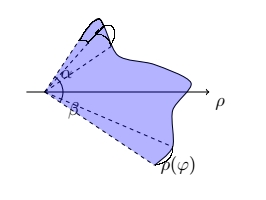
\includegraphics[scale=1]{sector.jpg}
\end{figure}
Оскільки $\rho \in C([\alpha,\beta]$, то $\rho \in C([\varphi_{j-1}, \varphi_j])$, тоді за Th. Вейєрштрасса, маємо:\\
$\rho(\varphi_j^*) = \huge \sup_{\varphi \in [\varphi_{j-1}, \varphi_j]} \rho(\varphi) \hspace{1.5cm} \rho(\varphi_{j*}) = \huge \inf_{\varphi \in [\varphi_{j-1}, \varphi_j]} \rho(\varphi)$\\
Сектори $Sec(\rho(\varphi_{j*}), [\varphi_{j-1}, \varphi_j])$, $Sec(\rho(\varphi^*_{j}), [\varphi_{j-1}, \varphi_j])$ мають таке співвідношення\\
$Sec(\rho(\varphi_{j*}), [\varphi_{j-1}, \varphi_j]) \subset Sec(\rho, [\varphi_{j-1}, \varphi_j]) \subset Sec(\rho(\varphi^*_{j}), [\varphi_{j-1}, \varphi_j])$\\
Тоді\\
$S(Sec(\rho(\varphi_{j*}), [\varphi_{j-1}, \varphi_j])) \leq S(Sec(\rho, [\varphi_{j-1}, \varphi_j])) \leq (Sec(\rho(\varphi^*_{j}), [\varphi_{j-1}, \varphi_j]))$\\
Причому \\ 
$S(Sec(\rho(\varphi_{j*}), [\varphi_{j-1}, \varphi_j])) = \dfrac{1}{2} \rho^2(\varphi_{j*}) (\varphi_{j} - \varphi_{j-1}) = \\ = \dfrac{1}{2} \huge \sup_{\varphi \in [\varphi_{j-1}, \varphi_j]} \rho^2(\varphi) (\varphi_{j} - \varphi_{j-1})$\\
$S(Sec(\rho(\varphi^*_{j}), [\varphi_{j-1}, \varphi_j])) = \dfrac{1}{2} \rho^2(\varphi^*_{j}) (\varphi_{j} - \varphi_{j-1}) = \\ = \dfrac{1}{2} \huge \inf_{\varphi \in [\varphi_{j-1}, \varphi_j]} \rho^2(\varphi) (\varphi_{j} - \varphi_{j-1})$\\
Тоді\\
$\huge \dfrac{1}{2} \inf_{\varphi \in [\varphi_{j-1}, \varphi_j]} \rho^2(\varphi) (\varphi_{j} - \varphi_{j-1}) \leq S(Sec(\rho, [\varphi_{j},\varphi_{j-1}])) \leq \\ \leq \dfrac{1}{2} \sup_{\varphi \in [\varphi_{j-1}, \varphi_j]} \rho^2(\varphi) (\varphi_{j} - \varphi_{j-1})$\\
Площа сектору - адитивна. Тоді за Th. Радона-Никодима, маємо:\\
$S(Sec(\rho, [a,b])) = \dfrac{1}{2} \huge \int\displaylimits_\alpha^\beta \rho^2(\varphi)\,d\varphi$
\bigline
Підсумуємо
\begin{theorem}
Криволінійний сектор $Sec(\rho, [a,b])$ є квадрованою (залишаємо це фактом), а її площа\\
$S(Sec(\rho, [a,b])) = \dfrac{1}{2} \huge \int\displaylimits_\alpha^\beta \rho^2(\varphi)\,d\varphi$
\bigline
\end{theorem}

\begin{example}
Знайдемо площу фігури, що задається таким рівнянням: $(x^2+y^2)^2 = 2xy$\\
Варто перейти до полярок, тому $x = \rho \cos \varphi$, $y = \rho \sin \varphi$\\
$\Rightarrow \rho^4 = 2 \rho^2 \cos \varphi \sin \varphi$\\
$\Rightarrow \rho = \sqrt{\sin 2\varphi}$
\begin{figure}[H]
\centering
\begin{tikzpicture}
  \draw[thick,->,>=latex] (-2,0)--(2.5,0) node[above] {$x$};
  \draw[thick,->,>=latex] (0,-2)--(0,2) node[left] {$y$};
  \draw[domain=0:90,scale=1.5,samples=500, name path = A] plot (\x:{sqrt(sin(2*\x))});
  \draw[domain=180:270,scale=1.5,samples=500, name path = B] plot (\x:{sqrt(sin(2*\x))});
  
  \tikzfillbetween[of=A and B]{blue, opacity = 0.3};
\end{tikzpicture}
\caption*{І чверть намальована кутами $\varphi \in \left[ 0, \dfrac{\pi}{2} \right]$, ІV чверть - кутами $\varphi \in \left[ \pi, \dfrac{3\pi}{2} \right]$}
\end{figure}
Оскільки ці два шмата симетричні, то я порахую площу однієї і помножу на два\\
$S_I = \dfrac{1}{2} \huge\int_0^{\pi/2} (\sqrt{\sin 2\varphi})^2 \,d \varphi = \dfrac{1}{2} \huge\int_0^{\pi/2} \sin 2\varphi \,d\varphi = -\dfrac{1}{4} \cos 2\varphi \Big|_0^{\pi/2} = \dfrac{1}{4}$\\
Отже, $S = 2 S_I = \dfrac{1}{2}$
\end{example}

\begin{example}
Знайти площу еліпса, що задана канонічним рівнянням\\
$\dfrac{x^2}{a^2} + \dfrac{y^2}{b^2} = 1$\\
Полярочка: $x = \rho \cos \varphi$, $y = \rho \sin \varphi$\\
$\dfrac{\rho^2 \cos^2 \varphi}{a^2} + \dfrac{\rho^2 \sin^2 \varphi}{b^2} = 1$\\
$\rho^2 = \dfrac{a^2b^2}{b^2 \cos^2 \varphi + a^2 \sin^2 \varphi}$\\
Тоді площа еліпса\\
$S = \dfrac{1}{2} \huge\int_{0}^{2\pi} \dfrac{a^2b^2}{b^2 \cos^2 \varphi + a^2 \sin^2 \varphi} \,d\varphi = \overset{\text{спробуйте самі )0) }}{\dots} = \pi ab$
\bigline
\end{example}

\subsubsection{Довжина кривої}
Задамо криву $\gamma$ - можна одним із способів:\\
\textbf{В просторі $\mathbb{R}^2$}\\
1) $\gamma: \{(x,y): x \in [a,b], y = f(x)\}$ - явна крива\\
2) $\gamma: \{(x,y): F(x,y) = 0\}$ - неявна крива\\
3) $\gamma: \{(x,y): x = x(t), y = y(t), t \in [a,b]\}$ - параметрична крива\\
4) $\gamma: \{(\varphi, \rho): \varphi \in [\alpha,\beta], \rho = \rho(\varphi)\}$ - крива в полярних координатах\\
5) $\gamma: \{(x,y,z): x = x(t), y = y(t), z = z(t), t \in [a,b]\}$ - параметрична крива

Представимо, що маємо криву $\gamma$. По-перше зробимо розбиття відрізка $[a,b]$\\
$a = x_0 < x_1 < x_2 < \dots < x_{n-1} = x_n = b$\\
По-друге, з'єднаємо точки кривої $\gamma$ послідовно \textbf{ламаною}, які будуть вписаними в криву $\gamma$

\begin{figure}[H]
\centering
\begin{tikzpicture}
\draw[thick, ->] (-0.5,0)--(6,0);
\draw[thick, gray] plot [smooth] coordinates {(0,1.5) (1.5,0.5) (3,2.5) (4,1.5) (5,2) (5.5,1)} node[anchor = west] {$\gamma$};
\draw (0,-2pt)--(0,2pt) node[anchor = north] {$a$};
\draw (1,-2pt)--(1,2pt) node[anchor = north] {$x_1$};
\draw (2,-2pt)--(2,2pt) node[anchor = north] {$x_2$};
\draw (4.5,-2pt)--(4.5,2pt) node[anchor = north] {$x_{n-1}$};
\draw (5.5,-2pt)--(5.5,2pt) node[anchor = north] {$b$};

\draw (0,1.5)--(1,0.65) -- (2,1.05) -- (3,2.5) -- (4,1.5) -- (4.5,1.75) -- (5.5,1);
\end{tikzpicture}
\end{figure}

\begin{definition}
Криву $\gamma$ будемо називати \textbf{спрямованою}, якщо множина довжин вписаних в неї ламаних буде обмеженою. А \textbf{довжиною} спрямованої кривої називають точну верхню межу довжин вписаних в неї ламаних
\end{definition}

Розглянемо функцію $y = f(x), x \in [a,b]$ та $f$ - диференційована\\
Знайдемо довжину кривої на $[a,b]$. Розглянемо ламану на $[x_1,x_2]$\\
За Th. Лагражна, $\exists c_{1,2} \in (x_1,x_2): f'(c_{1,2}) = \dfrac{f(x_2) - f(x_1)}{x_2-x_1}$\\
Рівняння частини ламаної має вигляд:\\
$y = \dfrac{f(x_2)-f(x_1)}{x_2-x_1}(x-x_1) + f(x_1)$\\
Довжина відрізку:\\
$l_{(x_1,x_2)} = \sqrt{(x_2-x_1)^2 + (f(x_2)-f(x_1))^2} = (x_2-x_1) \sqrt{1 + \left( \dfrac{f(x_2)-f(x_1)}{x_2-x_1} \right)^2} = \\ = (x_2-x_1) \sqrt{1+(f'(c_{1,2}))^2}$\\
Тоді сумарна довжина дорівнює\\
$l_{[a,b]} = \huge \sum_{j=1}^n \sqrt{1 + (f'(c_{j-1,j}))^2} (x_j-x_{j-1})$\\
Оскільки $f$ - диференційована, $f \in C([a,b])$, тоді $f$ - обмежена, тобто $\exists M: \sqrt{1+ (f'(x))^2} \leq M$\\
Отже, $l \leq \huge \sum_{j=1}^n M(x_j-x_{j-1}) = M(b-a)$ - свідчить про спрямованість кривої
\bigline
Перед тим як знаходити довжину кривої $\gamma$, що задана $y = f(x)$, спробуємо виконати це для параметрично заданої функції\\
$\gamma: \begin{cases}
 x = x(t) \\ y = y(t) \\ z = z(t)
 \end{cases}$\\
Довжина кривої $l_{[\alpha,\beta]}, [\alpha,\beta] \subset [a,b]$ - це довжина шляху за час $\beta - \alpha$. Тоді з фізичних міркувань (привіт, Калита)\\
$|\vec{v}|_{\min} (\beta - \alpha) \leq l_{[\alpha, \beta]} \leq |\vec{v}|_{\max} (\beta - \alpha)$\\
А швидкість $\vec{v} = (x'(t),y'(t),z'(t))$, тоді $|\vec{v}(t)| = \sqrt{(x'(t))^2+(y'(t))^2+(z'(t))^2}$\\
Тоді маємо:\\
$\huge \inf_{t \in [\alpha,\beta]} \sqrt{(x'(t))^2+(y'(t))^2+(z'(t))^2} (\beta - \alpha) \leq l_{[\alpha,\beta]} \leq \\ \leq \sup_{t \in [\alpha,\beta]} \sqrt{(x'(t))^2+(y'(t))^2+(z'(t))^2} (\beta - \alpha)$\\
А оскільки довжина - адитивна величина, то за Th. Радона-Никодима:\\
$l_\gamma = \huge \int\displaylimits_a^b \sqrt{(x'(t))^2+(y'(t))^2+(z'(t))^2} \,dt$
\bigline
Для $\gamma: \begin{cases} x = x(t) \\ y = y(t) \end{cases}$ таке саме рівняння\\
$l_\gamma = \huge \int\displaylimits_a^b \sqrt{(x'(t))^2+(y'(t))^2} \,dt$
\bigline
Повернімось до $\gamma: y = f(x)$\\
Такий тип еквівалентний параметричному рівнянню \\ $\begin{cases} x = t \\ y = f(t) \end{cases}, t \in [a,b]$\\
Тоді $\begin{cases} x' = 1 \\ y' = f'(t) \end{cases}$, а отже,\\
$l_j = \huge \int\displaylimits_a^b \sqrt{1+(f'(t))^2}\,dt$
\bigline
Залишилось розглянути випадок $\rho = \rho(\varphi), \varphi \in [\varphi_1,\varphi_2]$\\
Зв'язок між поляркою та декарткою задається такою системою\\
$\begin{cases} x = \rho \cos \varphi \\ y = \rho \sin \varphi \end{cases}$\\
Таким чином, ми маємо криву $\gamma: \begin{cases} x(\varphi) = \rho \cos \varphi \\ y(\varphi) = \rho \sin \varphi \end{cases}$\\
$x'(\varphi) = \rho' \cos \varphi - \rho \sin \varphi$\\
$y'(\varphi) = \rho' \sin \varphi + \rho \cos \varphi$\\
$\Rightarrow (x')^2 + (y')^2 + \dots = \rho^2 + (\rho')^2$\\
Отже, отримали таку формулу:\\
$l_\gamma = \huge\int\displaylimits_{\varphi_1}^{\varphi_2} \sqrt{(\rho(\varphi))^2 + (\rho'(\varphi))^2}\,d\varphi$
\bigline
\begin{example}
Знайти довжину кривої, що задана функцією \\ $y = \sqrt{2x-x^2} -1$ на проміжку $\left[ \dfrac{1}{4},1 \right]$\\
Знайдемо спочатку похідну цієї функції\\
$y' = \dfrac{1}{2 \sqrt{2x-x^2}} \cdot (2-2x) \Rightarrow (y')^2 = \dfrac{(1-x)^2}{2x-x^2}$\\
Тепер можна шукати довжину\\
$l = \huge\int_{1/4}^1 \sqrt{1 + \dfrac{(1-x)^2}{2x-x^2}}\,dx = \int_{1/4}^1 \dfrac{dx}{\sqrt{2x-x^2}} = \int_{1/4}^1 \dfrac{dx}{\sqrt{1-(x-1)^2}} = \\ = \arcsin(x-1) \Big|_{1/4}^1 = \arcsin \dfrac{3}{4}$
\bigline
\end{example}

\subsubsection{Об'єм фігури обертання}
Зафіксуємо деяку множину $A \subset \mathbb{R}^3$
\begin{definition}
\textbf{Зовіншім об'ємом} множини $A$ називають таке число
\begin{align*}
V^*(A) = \inf V(\text{об'єднання описаних паралелепіпедів})
\end{align*}
\end{definition}

\begin{definition}
\textbf{Внутрішньою площею} множини $A$ називають таке число
\begin{align*}
V_*(A) = \sup V(\text{об'єднання вписаних паралелепіпедів})
\end{align*}
\end{definition}
\begin{definition}
Множина $A$ називається \textbf{кубованою}, якщо
\begin{align*}
V^*(A) = V_*(A) = V(A)
\end{align*}
де $V(A)$ - об'єм кубованої множини $V$
\end{definition}

\begin{theorem}[Критерій кубованості]
Множина $A$ - кубована $\iff V(\partial A) = 0$\\
Де $\partial A = V^*(A) - V_*(A)$ - границя множини $A$\\
\textit{Усі доведення є аналогічні з квадрованими множинами}
\end{theorem}
А тепер задамо функцію $y = f(x), x \in [a,b]$ та $f \in C^1([a,b])$\\
Функція $f(x)$ та вісь $OX$ обмежують деяку фігуру\\
Обернімо цю фігуру навколо осі $OX$ - отримаємо \textbf{тіло обертання}, яке є кубованим\\
\textit{Доведення аналогічне з доведенням квадрованості криволінійної трапеції}
\begin{figure}[H]
\centering
\begin{tikzpicture}
\draw[thick, ->] (0,0)--(5,0) node[anchor = north] {$x$};
\draw [name path = A, thick] plot [smooth] coordinates {(0,1.5) (1,1.2) (2,0) (3,-1) (4,-0.5)} node[anchor = west] {$f$};
\end{tikzpicture}
\qquad
\begin{tikzpicture}
\draw[thick, ->] (0,0)--(5,0) node[anchor = north] {$x$};
\draw [name path = A, thick] plot [smooth] coordinates {(0,1.5) (1,1.2) (2,0) (3,-1) (4,-0.5)};
\draw [name path = A, thick] plot [smooth] coordinates {(0,-1.5) (1,-1.2) (2,0) (3,1) (4,0.5)};
\draw (0,0) ellipse (0.25 and 1.5);
\draw (4,0) ellipse (0.1 and 0.5);
\end{tikzpicture}
\end{figure}

Час знайти, як обчислити об'єм\\
$\forall [\alpha, \beta] \subset [a,b]:$ об'єм частини тіла обертання $V_{[\alpha,\beta]}$ задовільняє нерівності\\
Нагадую, що $V_{\text{циліндр}} = \pi R^2 H$\\
$V_{[\alpha,\beta]} \leq V_{\text{описаного циліндра}} = \pi \huge \underset{\text{радіус квадрат}}{\sup_{x \in [\alpha, \beta]} f^2(x)} \underset{\text{висота}}{(\beta - \alpha)}$\\
$V_{[\alpha,\beta]} \geq V_{\text{вписаного циліндра}} = \pi \huge \underset{\text{радіус квадрат}}{\inf_{x \in [\alpha, \beta]} f^2(x)} \underset{\text{висота}}{(\beta - \alpha)}$
\begin{figure}[H]
\centering
\begin{tikzpicture}
\draw[thick, ->] (0,0)--(5,0) node[anchor = north] {$x$};
\draw [name path = A, thick] plot [smooth] coordinates {(0,1.5) (1,1.2) (2,0) (3,-1) (4,-0.5)};
\draw [name path = A, thick] plot [smooth] coordinates {(0,-1.5) (1,-1.2) (2,0) (3,1) (4,0.5)};
\draw (0,0) ellipse (0.25 and 1.5);
\draw (0.35,0) ellipse (0.2 and 1.4);
\draw (4,0) ellipse (0.1 and 0.5);
\end{tikzpicture}
\caption*{Ліворуч маємо частину тіла обертання. А тепер спробуйте візуалізувати циліндр, який охоплює це тіло, та цілиндр, який всередині тіла}
\end{figure}

Отже, за Th. Радона-Нікодима, отримаємо:\\
$V_{[a,b]} = \huge \pi \int\displaylimits_a^b f^2(x)\,dx$
\bigline
Можна також мати функцію $x = g(y), y \in [a,b]$. Така функція та вісь $OY$ обмежує деяку фігуру\\
Якщо будемо фігуру обертати навколо $OY$, то отримаємо аналогічну формулу\\
$V_{[a,b]} = \huge \pi \int\displaylimits_a^b g^2(y)\,dy$
\bigline

\begin{example}
Обчислити об'єм тіла, що було отримано в результаті обертання $f(x) = \sin x, x \in [0,\pi]$ навколо $OX$
\begin{figure}[H]
\centering
\begin{tikzpicture}[scale = 2]
\draw[thick, ->] (-0.5,0)--(3.5,0) node[anchor = north] {$x$};
\draw[thick, ->] (0,-1.5)--(0,1.5) node[anchor = east] {$y$};
\draw[thick, domain=0:pi, variable=\x, samples = 100] plot({\x}, {sin(deg(\x))});
\draw[dashed, domain=0:pi, variable=\x, samples = 100] plot({\x}, {-sin(deg(\x))});
\draw[dashed] ({pi/2},0) ellipse (0.1 and 1);
\end{tikzpicture}
\end{figure}
$V = \pi \huge\int_0^\pi \sin^2 x \,dx = \dfrac{\pi}{2} \huge\int_0^\pi 1 - \cos 2x \,dx = \dfrac{\pi}{2} \left(x - \dfrac{1}{2} \sin 2x \right) \Big|_0^\pi = \dfrac{\pi^2}{2}$
\end{example}

\subsubsection{Об'єм фігури через площу поперечного перерізу}
Задано $A$ - кубована множина, для якої відомо, що\\
$A \ni (x,y,z)$, $z_1 \leq z \leq z_2$, $A$ - обмежена\\
$\forall z_0 \in [z_1,z_2]:$ відома площа перетину множини $A$ та площини $z=z_0$, що дорівнює $S(z_0)$
\begin{figure}[H]
\centering
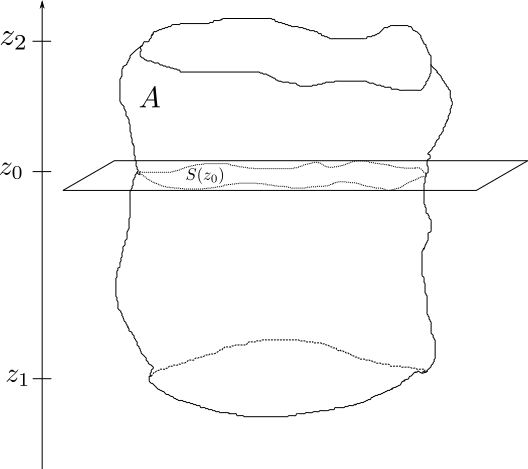
\includegraphics[scale=0.6]{volume_with_surface.png};
\end{figure}

$\forall [z_3,z_4] \subset [z_1,z_2]:$\\
Проведемо площини $z_3,z_4$ - отримаємо площі $S(z_3),S(z_4)$ та деякий об'єм $V_{[z_3,z_4]}$, об'єм між цими площинами, що має таку оцінку:\\
$V_{[z_3,z_4]} \leq V_{\text{циліндра з max площею перерізу}} = \huge \underset{\text{площа основи}}{\sup_{z \in [z_3,z_4]} S(z)} \cdot \underset{\text{висота}}{(z_4-z_3)}$\\
$V_{[z_3,z_4]} \geq V_{\text{циліндра з min площею перерізу}} = \huge \underset{\text{площа основи}}{\inf_{z \in [z_3,z_4]} S(z)} \cdot \underset{\text{висота}}{(z_4-z_3)}$\\
Отже, за Th. Радона-Нікодима, отримаємо:\\
$V_{[z_1,z_2]} = \huge\int\displaylimits_{z_1}^{z_2} S(z)\,dz$
\bigline

\begin{example}
Знайти об'єм еліпсоїда, що задана канонічним рівнянням:\\
$\dfrac{x^2}{a^2} + \dfrac{y^2}{b^2} + \dfrac{z^2}{c^2} = 1$
\begin{figure}[H]
\centering
\begin{tikzpicture}
\node at (0.5,2.8) {$c$};
\node at (0.5,-2.8) {$-c$};
\draw (0,0) ellipse (1.5 and 2.5);
\draw[dashed] (0,0) ellipse (1.5 and 0.25);
\draw[thick, ->] (0,-3)--(0,3) node[anchor = east] {$z$};
\end{tikzpicture}
\caption*{Ми скоро знайдемо площу штрихованого еліпса, який можемо переміщати вздовж $OZ$}
\end{figure}
Якщо перетинати цей еліпсоїд площиною $z=z_0$, як це було в попередньому малюну, то всередині буде утворюватись еліпс, від якої ми можемо знайти площу\\
Перед цим необхідно знайти сам еліпс. Зробимо це таким чином\\
$\dfrac{x^2}{a^2} + \dfrac{y^2}{b^2} = 1 - \dfrac{z^2}{c^2}$\\
$\dfrac{x^2}{a^2 \left(1 - \dfrac{z^2}{c^2} \right)} + \dfrac{y^2}{b^2 \left(1 - \dfrac{z^2}{c^2} \right)} = 1$\\
Отримали канонічне рівняння еліпса, який залежить від $z$\\
Сторони еліпса: $a_1(z) = a \sqrt{1 - \dfrac{z^2}{c^2}}$, $b_1(z) = b \sqrt{1 - \dfrac{z^2}{c^2}}$\\
Площа еліпса: $S(z) = \pi a_1(z) b_1(z) = \pi ab \left(1 - \dfrac{z^2}{c^2} \right)$\\
А тепер можемо й об'єм знайти\\
$V = \huge\int_{-c}^c \pi ab \left( 1 = \dfrac{z^2}{c^2} \right)\,dz = \pi ab \left(z - \dfrac{1}{c^2} \dfrac{z^3}{3} \right) \Big|_{-c}^c = \dfrac{4}{3}abc$

\end{example}
\newpage

\section{Невласні інтеграли}
\subsection{Основні означення}
Розглянемо три випадки:\\
I. Задана така функція $f: [a,+\infty) \to \mathbb{R}$, що $\forall b \in [a,+\infty): f \in D([a,b])$
\begin{definition}
\textbf{Невласним інтегралом I роду} називають такий вираз (якщо границя існує)
\begin{align*}
\int\displaylimits_a^\infty f(x)\,dx = \lim_{b \to +\infty} \int\displaylimits_a^b f(x)\,dx
\end{align*}
\end{definition}

\begin{remark}
Аналогічно визначається для $f: (-\infty,b] \to \mathbb{R}$
\end{remark}

II. Задана така функція $f: [a,b) \to \mathbb{R}$, що $\forall \varepsilon > 0: f \in D([a,b-\varepsilon])$
\begin{definition}
\textbf{Невласним інтегралом II роду} називають такий вираз (якщо границя існує)
\begin{align*}
\int\displaylimits_a^b f(x)\,dx = \lim_{\varepsilon \to 0} \int\displaylimits_a^{b-\varepsilon} f(x)\,dx
\end{align*}
\end{definition}

\begin{remark}
Аналогічно визначається для $f: (a,b] \to \mathbb{R}$
\end{remark}

\begin{definition}
Якщо границя існує, то невласний інтеграл називається \textbf{збіжним}. Інакше - \textbf{розбіжним}
\end{definition}

III. Задана $f: [a, \omega) \to \mathbb{R}$, де $\left[ \begin{gathered} \omega = +\infty \\ \omega = b \end{gathered} \right.$\\
Але цього разу на $[a,\omega)$ виникають особливі точки для функції $f$\\
$a < c_1 < c_2 < \dots < c_k < \omega$\\
Дізнаймось, як тоді визначити $\huge\int\displaylimits_a^\omega f(x)\,dx$\\
Ми розглянемо інші точки \\ $a < \textcolor{red}{t_1} < c_1 < \textcolor{red}{t_2} < c_2 < \dots < \textcolor{red}{t_k} < c_k < \textcolor{red}{t_{k+1}} < \omega$\\
Це робиться, оскільки ми вже навчились інтегрувати ІІ рід, а останній доданок може бути й І рід. Рахується інтеграл в цьому випадку таким чином\\
$\huge\int\displaylimits_a^\omega f(x)\,dx = \int\displaylimits_a^{t_1} f(x)\,dx + \int\displaylimits_{t_1}^{c_1} f(x)\,dx + \int\displaylimits_{c_1}^{t_2} f(x)\,dx + \dots + \\ + \int\displaylimits_{c_k}^{t_{k+1}} f(x)\,dx + \int\displaylimits_{t_{k+1}}^{\omega} f(x)\,dx$\\


Доведімо швиденько адитивність невласних інтегралів\\
$f \in D([a,A]), \forall A \in [a,\omega)$ та $\huge \int\displaylimits_a^\omega f(x)\,dx$ - збіжний\\
Зафіксуємо довільну т. $t \in [a,\omega)$, тоді:\\
$\huge \int\displaylimits_a^\omega f(x)\,dx = \huge \lim_{A \to \omega^-} \int\displaylimits_a^A f(x)\,dx = \lim_{A \to \omega^-} \left(\int\displaylimits_a^t f(x)\,dx + \int\displaylimits_t^A f(x)\,dx \right) = \\ = \int\displaylimits_a^t f(x)\,dx + \int\displaylimits_t^\omega f(x)\,dx$\\
А тепер треба пересвідчитись, що працює незалежність від вибору $t_1,t_2,\dots,t_{k+1}$\\
Розглянемо $t,t' \in (a,\omega)$ та $t < t'$\\
$\huge\int\displaylimits_a^\omega f(x)\,dx = \int\displaylimits_a^{t'} d(x)\,dx + \int\displaylimits_{t'}^{\omega} f(x)\,dx = \int\displaylimits_a^{t} f(x)\,dx + \int\displaylimits_{t}^{t'} f(x)\,dx + \int\displaylimits_{t'}^{\omega} f(x)\,dx = \\
= \int\displaylimits_{a}^{t} f(x)\,dx + \int\displaylimits_{t}^{t'} f(x)\,dx + \int\displaylimits_{t'}^{\omega} f(x)\,dx = \int\displaylimits_{a}^{t} f(x)\,dx + \int\displaylimits_{t}^{\omega} f(x)\,dx = \huge\int\displaylimits_a^\omega f(x)\,dx$\\
Тобто визначення невласного інтегралу не залежить від вибору точок $t_1,t_2,\dots,t_{k+1}$

\begin{proposition}[Властивості]
1. Якщо $f \in D([a,b])$, то невласний інтеграл дорівнює визначеному інтегралу\\
\begin{pfNoTh}
$\huge\int\displaylimits_a^b f(x)\,dx = \huge \lim_{A \to b^-} \int\displaylimits_a^A f(x)\,dx = $\\
Оскільки $f \in D([a,b])$, то маємо первісну $F \in C([a,b]): F(t) = \huge\int\displaylimits_a^t f(x)\,dx$\\
$= \huge \lim_{A \to b^-} (F(A)-f(a)) = F(b) - F(a) = \huge\int\displaylimits_a^b f(x)\,dx$
\end{pfNoTh}

2. Всі властивості визначеного інтегралу копіюються на невласні інтеграли за умовою, що задані невласні інтеграли є збіжними!
\end{proposition}

\begin{example} Трошки покалькулюємо деякі інтеграли\\
$\huge\int_0^1 \ln x \,dx = \huge \lim_{\varepsilon \to 0} \int_{0+\varepsilon}^1 \ln x \,dx \boxed{=}$\\
Інтегруємо частинами: $u = \ln x$, $dv = dx$\\
$\boxed{=} \huge\lim_{\varepsilon \to 0} \left(x \ln x \Big|_{0+\varepsilon}^1 - x \Big|_{0+\varepsilon}^1 \right) = \lim_{\varepsilon \to 0} \left( -\varepsilon \ln \varepsilon - 1 + \varepsilon \right) = \\ = \lim_{\varepsilon \to 0} \dfrac{\ln \varepsilon}{-\dfrac{1}{\varepsilon}} + \lim_{\varepsilon \to 0} (\varepsilon - 1) \overset{\text{перший Лопіталем}}{=} \lim_{\varepsilon \to 0} \dfrac{\dfrac{1}{\varepsilon}}{\dfrac{1}{\varepsilon^2}} - 1 = -1$\\
Інтеграл - збіжний та, ба більше, приймає приємне значення
\bigline
$\huge\int_0^{\infty} x\,dx = \lim_{b \to \infty} \int_0^b x\,dx = \lim_{b \to \infty} \dfrac{x^2}{2} \Big|_0^b = \lim_{b \to \infty} \dfrac{b^2}{2} = \infty$\\
Інтеграл - розбіжний, ну ок
\bigline
Проте не всі невласні інтеграли визначаються на збіжність шляхом стандратного обчислення. Тому люди вигадали інші підрозділи\\
\end{example}


\subsection{Еталонні інтеграли}
Вони вам дуже допоможуть, коли будете використовувати теореми на визначення збіжності, що будуть надані знизу\\
1. $\huge\int_1^{+\infty} \dfrac{dx}{x^\alpha} = \huge\lim_{A \to +\infty} \int_1^A x^{-\alpha} \,dx =$\\
при $\alpha = 1$ маємо: $= \huge\lim_{A \to +\infty} \ln x \Big|_1^A = \lim_{A \to +\infty} \ln A = +\infty$\\
при $\alpha \neq 1$ маємо: $= \huge\lim_{A \to +\infty} \dfrac{x^{-\alpha+1}}{-\alpha+1} \Big|_1^A =$\\
\text{ } \hspace{0.4cm} при $\alpha < 1$: $= \huge\lim_{A \to +\infty} \dfrac{1}{1-\alpha} (A^{1-\alpha} - 1) = +\infty$\\
\text{ } \hspace{0.4cm} при $\alpha > 1$: $= \huge\lim_{A \to +\infty} \dfrac{1}{1-\alpha} (\dfrac{1}{A^{\alpha-1}} - 1) = \dfrac{1}{\alpha - 1}$
\bigline
2. $\huge\int_0^1 \dfrac{dx}{x^{\alpha}} = \huge\lim_{\varepsilon \to 0^+} \int_\varepsilon^1 x^{-\alpha}\,dx = $\\
при $\alpha = 1$ маємо: $= \huge\lim_{\varepsilon \to 0^+} \ln x \Big|_\varepsilon^1 = \lim_{\varepsilon \to 0^+} (-\ln \varepsilon) = +\infty$\\
при $\alpha \neq 1$ маємо: $= \huge\lim_{\varepsilon \to 0^+} \dfrac{x^{-\alpha+1}}{-\alpha+1} \Big|_\varepsilon^1 =$\\
\text{ } \hspace{0.4cm} при $\alpha > 1$: $= \huge\lim_{\varepsilon \to 0^+} \dfrac{1}{1-\alpha} (1 - \dfrac{1}{\varepsilon^{\alpha-1}}) = +\infty$\\
\text{ } \hspace{0.4cm} при $\alpha < 1$: $= \huge\lim_{\varepsilon \to 0^+} \dfrac{1}{1-\alpha} (1 - \varepsilon^{1-\alpha}) = \dfrac{1}{1-\alpha}$
\bigline
3. $\huge\int_1^{+\infty} a^x\,dx = \dfrac{a^x}{\ln a} \Big|_1^{+\infty} =$\\
при $a \geq 1$ маємо: $= +\infty$\\
при $0 < a < 1$ маємо: $= \dfrac{1}{-\ln a}$
\bigline
ОТЖЕ,\\
$\huge\int_1^{+\infty} \dfrac{dx}{x^\alpha}$ - $\left[ \begin{gathered} \text{збіжний, якщо } \alpha > 1 \\ \text{розбіжний, якщо } \alpha \leq 1 \\ \end{gathered} \right.$\\
$\huge\int_0^{1} \dfrac{dx}{x^\alpha}$ - $\left[ \begin{gathered} \text{збіжний, якщо } \alpha < 1 \\ \text{розбіжний, якщо } \alpha \geq 1 \\ \end{gathered} \right.$\\
$\huge\int_1^{+\infty} a^x\,dx$ - $\left[ \begin{gathered} \text{збіжний, якщо } 0 < a < 1 \\ \text{розбіжний, якщо } a \geq 1 \\ \end{gathered} \right.$\\
Користуйтесь)\\

\subsection{Дослідження на збіжність/розбіжність}
\begin{theorem}[Критерій Коші]
Задана функція $f \in D([a,A]), \forall A \in [a,\omega)$. Тут $\omega = \left[ \begin{gathered}  b \\ +\infty \end{gathered} \right.$\\
$\huge\int\displaylimits_a^\omega f(x)\,dx$ - збіжний $\iff \forall \varepsilon > 0: \exists \left[ \begin{gathered} \delta \text{,якщо } \omega = b \\ \Delta \text{,якщо } \omega = +\infty \end{gathered} \right. : \\ \forall \left[ \begin{gathered} A_1,A_2 \in (b-\delta,b) \text{,якщо } \omega = b \\ A_1,A_2 \in (\Delta, +\infty) \text{,якщо } \omega = +\infty \end{gathered}  \right. \Rightarrow \abs{\huge\int\displaylimits_{A_1}^{A_2} f(x)\,dx} < \varepsilon$
\end{theorem}

\begin{pf}
Позначимо $\huge\int\displaylimits_a^t f(x)\,dx = F(t)$\\
$\huge\int\displaylimits_a^\omega f(x)\,dx = \lim_{A \to \omega} F(A)$ - збіжний $\overset{\text{критерій Коші для ліміта}}{\iff}$\\
$\forall \varepsilon > 0: \exists \left[ \begin{gathered} \delta \text{,якщо } \omega = b \\ \Delta \text{,якщо } \omega = +\infty \end{gathered} \right. :  \forall \left[ \begin{gathered} A_1,A_2 \in (b-\delta,b) \text{,якщо } \omega = b \\ A_1,A_2 \in (\Delta, +\infty) \text{,якщо } \omega = +\infty \end{gathered}  \right. \Rightarrow \\ \abs{F(A_1)-F(A_2)} = \abs{\huge\int\displaylimits_{A_1}^{A_2} f(x)\,dx} < \varepsilon$
\end{pf}
\bigline

\subsubsection{Дослідження для додатних функції}
Тобто в цьому підпідрозділі розглядаються функції $f(x), g(x), \dots \geq 0$ на всьому області визначення
\begin{theorem}[Ознака порівняння в нерівностях]
Задані функції $f,g \in D([a,A]): \forall A \in [a,\omega)$ - додатні. Відомо, що\\
$\exists c \in [a,\omega): \forall x \geq c: f(x) \leq g(x)$. Тоді\\
1) Якщо $\huge\int\displaylimits_a^\omega g(x)\,dx$ - збіжний, то $\huge\int\displaylimits_a^\omega f(x)\,dx$ - збіжний\\
2) Якщо $\huge\int\displaylimits_a^\omega f(x)\,dx$ - розбіжний, то $\huge\int\displaylimits_a^\omega g(x)\,dx$ - розбіжний\\
\end{theorem}

\begin{pf}
Маємо функції $F(t) = \huge\int\displaylimits_a^t f(x)\,dx$, $G(t) = \huge\int\displaylimits_a^t g(x)\,dx$\\
$f(x),g(x)$ - додатні, то $\forall x \in [a,\omega): f(x),g(x) \geq 0$, тоді $\forall t \in [a,\omega): F(t),G(t) \geq 0$\\
Зафіксуймо $t_1,t_2$, що $a < t_1 < t_2 < \omega$. Тоді\\
$F(t_2) = \huge\int\displaylimits_a^{t_2} f(x)\,dx = \huge\int\displaylimits_a^{t_1} f(x)\,dx + \huge\int\displaylimits_{t_1}^{t_2} f(x)\,dx \geq \huge\int\displaylimits_a^{t_1} f(x)\,dx = F(t_1)$\\
Таким чином, $F$ - неспадна функція. Аналогічно $G$ - неспадна функція\\
1) А тепер нехай відомо, що $\huge\int\displaylimits_a^\omega g(x)\,dx$ - збіжний, отже\\
$\huge\int\displaylimits_a^\omega g(x)\,dx = \huge \lim_{A \to \omega^-} G(A) \overset{G\text{ - неспадна}}{=} \sup_{t \in [a,\omega)} G(t)$\\
Оскільки $\exists c \in [a,\omega): \forall x \geq c: f(x) \leq g(x)$, то тоді $F(t) \leq G(t), \forall t \geq c$\\
А отже, $F(t) \leq \huge \sup_{t \in [a,\omega)} G(t)$\\
Через те, що $F(t)$ - обмежена та неспадна, то $\huge\exists \lim_{A \to \omega^-} F(A) = \int\displaylimits_a^\omega f(x)\,dx$ - збіжний\\
2) А тепер нехай відомо, що $\huge\int\displaylimits_a^\omega f(x)\,dx$ - розбіжний\\
!Якщо припустити, що інтеграл $\huge\int\displaylimits_a^\omega g(x)\,dx$ - збіжний, то за п. 1), інтеграл з $\huge\int\displaylimits_a^\omega f(x)\,dx$ - збіжний, що суперечить!\\
Таким чином, $\huge\int\displaylimits_a^\omega g(x)\,dx$ - розбіжний
\end{pf}
\\
\begin{example}
Дослідити на збіжність $\huge\int_0^1 \dfrac{\cos^2 x}{\sqrt{x}}\,dx$\\
Маємо $f(x) = \dfrac{\cos^2 x}{\sqrt{x}}$\\
Відомо, що $\cos^2 x \leq 1$. Встановимо функцію $g(x) = \dfrac{1}{\sqrt{x}}$\\
Тоді $\forall x \in (0,1]: f(x) \leq g(x)$\\
$\huge\int_0^1 \dfrac{1}{\sqrt{x}}\,dx$ - збіжний (еталон)\\
Отже, за ознакою порівняння, п. 1), $\huge\int_0^1 \dfrac{\cos^2 x}{\sqrt{x}}\,dx$ - збіжний
\\
\end{example}

\begin{theorem}[Ознака порівняння в границях]
Задані функції $f,g \in D([a,A]): \forall A \in [a,\omega)$ - строго додатні. Відомо, що\\
$\exists \huge \lim_{x \to \omega^-} \dfrac{f(x)}{g(x)} = L$. Тоді\\
1) Якщо $L \neq 0, \neq \infty$, то обидва $\huge\int\displaylimits_a^\omega f(x)\,dx$, $\huge\int\displaylimits_a^\omega g(x)\,dx$ - збіжні або розбіжні\\
2) Ящо $L = 0$, то зі збіжності $\huge\int\displaylimits_a^\omega g(x)\,dx$ випливає збіжність $\huge\int\displaylimits_a^\omega f(x)\,dx$
\end{theorem}
\begin{pf}
1) Розглянемо $L \neq 0$, але оскільки $f,g > 0$, то $L>0$\\
$\exists \huge \lim_{x \to \omega^-} \dfrac{f(x)}{g(x)} = L \iff$\\
$\forall \varepsilon > 0: \exists c \in [a,\omega): \forall x \geq c: \abs{\dfrac{f(x)}{g(x)} - L} < \varepsilon$\\
Розглянемо $\varepsilon = \dfrac{L}{2}$, тоді $\dfrac{L}{2} < \dfrac{f(x)}{g(x)} < \dfrac{3L}{2} \Rightarrow \dfrac{L}{2}g(x) < f(x) < \dfrac{3L}{2}g(x)$\\
Якщо $\huge\int\displaylimits_a^\omega g(x)\,dx$ - збіжний, то $\huge\int\displaylimits_a^\omega \dfrac{3L}{2} g(x)\,dx$ - збіжний, то $\huge\int\displaylimits_a^\omega f(x)\,dx$ - збіжний\\
Якщо $\huge\int\displaylimits_a^\omega f(x)\,dx$ - збіжний, то $\huge\int\displaylimits_a^\omega \dfrac{L}{2} g(x)\,dx$ - збіжний, то $\huge\int\displaylimits_a^\omega g(x)\,dx$ - збіжний\\
Це все за арифметичними властивостями збіжності та попередньою ознакою порівняння, п.1)\\
Тож $\huge\int\displaylimits_a^\omega f(x)\,dx$, $\huge\int\displaylimits_a^\omega g(x)\,dx$ - одночасно збіжні\\
Аналогічно можна довести однакову розбіжність, якщо починати нерівність зліва
\bigline
2) Розглянемо $L = 0$, то $\exists \huge \lim_{x \to \omega^-} \dfrac{f(x)}{g(x)} = 0 \iff$\\
$\forall \varepsilon > 0: \exists c \in [a,\omega): \forall x \geq c: \abs{\dfrac{f(x)}{g(x)}} < \varepsilon$\\
Розглянемо $\varepsilon = 1$, то тоді $f(x) < g(x), \forall x \geq c$, а це вже посилання на попередню теорему
\end{pf}
\\
\begin{example}
Дослідити на збіжність $\huge\int_{\textcolor{red}{0}}^{+\infty} \dfrac{\arctg x}{x^{\frac{1}{5}}}$\\
Маємо функцію $f(x) = \dfrac{\arctg x}{x^{\frac{1}{5}}}$\\
Візьміть функцію $g(x) = \dfrac{1}{x^{-\frac{4}{5}}}$\\
Тоді $\huge \lim_{x \to \textcolor{red}{0}} \dfrac{\dfrac{\arctg x}{x^{\frac{1}{5}}}}{\dfrac{1}{x^{-\frac{4}{5}}}} = \lim_{x \to 0} \dfrac{\arctg x}{x} \overset{\text{насл. І чудової}}{=} 1$\\
А тепер оскільки $\huge\int_0^{+\infty} \dfrac{1}{x^{-\frac{4}{5}}}$ - розбіжний (еталон), то за ознакою порівняння в лімітах, п. 1), $\huge\int_{\textcolor{red}{0}}^{+\infty} \dfrac{\arctg x}{x^{\frac{1}{5}}}$ - розбіжний
\\
\end{example}

\subsubsection{Дослідження для знакодовільних функцій}
\begin{definition}
Задана функція $f \in D([a;A]), \forall A \in [a,\omega)$\\
$\huge\int\displaylimits_a^\omega f(x)\,dx$ називається \textbf{абсолютно збіжним}, якщо $\huge\int\displaylimits_a^\omega |f(x)|\,dx$ - збіжний\\
$\huge\int\displaylimits_a^\omega f(x)\,dx$ називається \textbf{умовно збіжним}, якщо $\huge\int\displaylimits_a^\omega |f(x)|\,dx$ - розбіжний, але при цьому $\huge\int\displaylimits_a^\omega f(x)\,dx$ - збіжний
\end{definition}

\begin{remark}
Якщо $f \in D$, то $|f| \in D$. Тому з означенням все ок
\end{remark}

\begin{proposition}
Задана функція $f \in D([a;A]), \forall A \in [a,\omega)$\\
Відомо, що $\huge\int\displaylimits_a^\omega |f(x)|\,dx$ - збіжний. Тоді $\huge\int\displaylimits_a^\omega f(x)\,dx$ - збіжний
\end{proposition}

\begin{pf}
$\huge\int\displaylimits_a^\omega |f(x)|\,dx$ - збіжний. За критерієм Коші,\\
$\forall \varepsilon > 0: \exists \left[ \begin{gathered} \delta \text{,якщо } \omega = b \\ \Delta \text{,якщо } \omega = +\infty \end{gathered} \right. : \forall \left[ \begin{gathered} A_1,A_2 \in (b-\delta,b) \text{,якщо } \omega = b \\ A_1,A_2 \in (\Delta, +\infty) \text{,якщо } \omega = +\infty \end{gathered}  \right. \Rightarrow \\ \abs{\huge\int\displaylimits_{A_1}^{A_2} |f(x)|\,dx} < \varepsilon$\\
$\abs{\huge\int\displaylimits_{A_1}^{A_2} \textcolor{red}{f(x)}\,dx} \leq \abs{\huge\int\displaylimits_{A_1}^{A_2} \textcolor{red}{|f(x)|}\,dx} < \varepsilon$\\
Тоді за критерієм Коші, $\huge\int\displaylimits_a^\omega f(x)\,dx$ - збіжний
\end{pf}

\begin{theorem}[Ознаки Абеля-Діріхле]
Задані функції $f,g \in D([a,A]), \forall A \in [a,\omega)$\\
Відомо, що обидва функції задовільняють одній з парі умов\\
\begin{tabular}{c | c}
$\huge \int\displaylimits_a^\omega f(x)\,dx$ - збіжний & $\exists M > 0: \forall A \in [a,\omega): \abs{\huge\int\displaylimits_a^A f(x)\,dx} < M$ \\
$g(x)$ - монотонна та обмежена & $g(x)$ - монотонна та $\huge \lim_{x \to \omega} g(x) = 0$ \\
\textit{ознаки Абеля} & \textit{ознаки Діріхле}
\end{tabular}\\
Тоді $\huge\int\displaylimits_a^\omega f(x)g(x)\,dx$ - збіжний
\end{theorem}

\begin{pf}
Доводимо блок Абеля. Додатково вимагаємо, що $g \in C^1$ (лише для спрощення доведеня). Маємо\\
$\huge\int\displaylimits_a^A f(x)g(x)\,dx \boxed{=}$\\
$u = g(x) \Rightarrow u' = g'(x)\,dx$\\
$dv = f(x)\,dx \Rightarrow v = \huge\int_a^x f(t)\,dt$\\
$\boxed{=} \huge \left( g(x) \int\displaylimits_a^x f(t)\,dt \right)\Big|_a^A - \int\displaylimits_a^A \left( \int\displaylimits_a^x f(t)\,dt \right) g'(x)\,dx \boxed{\boxed{=}}$\\
Перший доданок:\\
$\huge \left( g(x) \int\displaylimits_a^x f(t)\,dt \right)\Big|_a^A = g(A) \huge\int\displaylimits_a^A f(t)\,dt$\\
Другий доданок:\\
Маємо $\huge\int\displaylimits_a^x f(t)\,dt \in C([a,A])$\\
Також оскільки $g$ - монотонна, то тоді $g'$ - знакостала\\
Застосуємо Th. про середнє II - тобто $\exists \textcolor{red}{c} \in [a,A]:$\\
$\huge \int\displaylimits_a^A \left( \int\displaylimits_a^x f(t)\,dt \right) g'(x)\,dx =\huge\int\displaylimits_a^{\textcolor{red}{c}} f(t)\,dt \int\displaylimits_a^A g'(x)\,dx = \huge\int\displaylimits_a^{\textcolor{red}{c}} f(t)\,dt (g(A)-g(a))$\\
$\boxed{\boxed{=}} g(A) \huge\int\displaylimits_a^A f(t)\,dt - (g(A)-g(a))\int\displaylimits_a^c f(t)\,dt$\\
Що буде тепер, якщо $A \to \omega$\\
$\huge\int\displaylimits_a^A f(t)\,dt \to \huge\int\displaylimits_a^\omega f(t)\,dt$ - збіжний за умовою. Також $g(A)$ - якесь число, бо $g$ - обмежена та монотонна\\
Тоді $g(A) \huge\int\displaylimits_a^\omega f(t)\,dt$ - перший доданок - збіжний\\
$\huge\int\displaylimits_a^c f(t)\,dt$ - другий доданок - визначений інтеграл, тобто скінченне значення\\
Остаточно, $\exists \huge\lim_{A \to \omega} \int\displaylimits_a^A f(x)g(x)\,dx$, а тому збіжний
\bigline
Блок Діріхле доводиться аналогічно
\end{pf}\\

\begin{example}[Важливий]
Дослідимо на збіжність $\huge\int_0^{+\infty} \dfrac{\sin x}{x}\,dx$ - \textbf{інтеграл Діріхле}\\
Маємо $f(x) = \sin x$, $g(x) = \dfrac{1}{x}$\\
До речі, $\huge\lim_{x \to 0} \dfrac{\sin x}{x} = 1$, тож $x = 0$ - усувна точка, тобто вона не є особливою точкою\\
Тому $\forall A \in [0,+\infty): \dfrac{\sin x}{x} \in D([0,A])$\\
Перевіримо умови Діріхле\\
$\abs{\huge\int_0^{A} f(x)\,dx} = \abs{\huge\int_0^A \sin x \,dx} = |-\cos A + \cos 0| \leq 2$, виконано $\forall A \geq 0$ - встановимо $M = 2$\\
Перша умова виконана\\
$g(x) = \dfrac{1}{x}$ - монотонна, $\huge\lim_{x \to \infty} \dfrac{1}{x} = 0$\\
Друга умова виконана\\
Таким чином, за ознакою Діріхле,  $\huge\int_0^{+\infty} \dfrac{\sin x}{x}\,dx$  - збіжний
\bigline
Дослідимо тепер на абсолютну збіжність\\
!Припустимо, що це, дійсно, абсолютно збіжний інтеграл, тобто\\
$\huge\int_0^{+\infty} \abs{\dfrac{\sin x}{x}}\,dx = \huge\int_0^{+\infty} \dfrac{|\sin x|}{x}\,dx$ - збіжний\\
Зауважимо, що $|\sin x| \geq \sin^2 x$\\
Тоді за ознакою порівняння в нерівностях, $\huge\int_0^{+\infty} \dfrac{\sin^2 x}{x}\,dx$ - збіжний\\
Тому збіжними будуть два інтеграли\\
$\huge\int_0^{+\infty} \dfrac{\sin^2 x}{x}\,dx = \huge\int_0^1 \dfrac{\sin^2 x}{x}\,dx + \huge\int_1^{+\infty} \dfrac{\sin^2 x}{x}\,dx = \\ =
\huge\int_0^1 \dfrac{\sin^2 x}{x}\,dx + \huge\int_1^{+\infty} \dfrac{1 - \cos^2 x}{x}\,dx = \huge\int_0^1 \dfrac{\sin^2 x}{x}\,dx + \huge\int_1^{+\infty} \dfrac{1}{x} - \dfrac{1+\cos 2x}{2x} \,dx = \\
= \huge\int_0^1 \dfrac{\sin^2 x}{x}\,dx + \huge\int_1^{+\infty} \dfrac{1}{2x} - \dfrac{\cos 2x}{2x} \,dx$\\
Звідси $\huge\int_1^{+\infty} \dfrac{1}{2x} \,dx$ та $\huge\int_1^{+\infty} \dfrac{1}{2x}-\dfrac{\cos 2x}{2x} \,dx$ - збіжні\\
Проте за еталоном, $\huge\int_1^{+\infty} \dfrac{1}{2x} \,dx$ НЕ є збіжним. Суперечність!\\
Отже, $\huge\int_0^{+\infty} \dfrac{\sin x}{x}\,dx$ - не збіжний абсолютно\\
Висновок: $\huge\int_0^{+\infty} \dfrac{\sin x}{x}\,dx$ - умовно збіжний
\bigline
\end{example}

\subsection{Невласний інтеграл в сенсі головного значення}
I. Розглянемо такий інтеграл
\begin{align*}
\int\displaylimits_{-\infty}^{+\infty} f(x)\,dx
\end{align*}
У неї з обох сторін проблеми. В стандартному невласному інтегралі це можна записати так. Тут $t \in \mathbb{R}$\\
$\huge\int\displaylimits_{-\infty}^{+\infty} f(x)\,dx = \huge\int\displaylimits_{-\infty}^{t} f(x)\,dx + \huge\int\displaylimits_{t}^{+\infty} f(x)\,dx = \lim_{B \to -\infty} \int\displaylimits_B^t f(x)\,dx + \lim_{A \to +\infty} \int\displaylimits_t^A f(x)\,dx = \\
= \lim_{\substack{A\to +\infty \\ B \to -\infty}} \int\displaylimits_B^A f(x)\,dx$\\
І це - незручно\\
Тому розглядають люди такий же інтеграл, але в сенсі головного значення
\begin{align*}
v.p. \int\displaylimits_{-\infty}^{+\infty} f(x)\,dx = \lim_{A \to \infty} \int\displaylimits_{-A}^A f(x)\,dx
\bigline
\end{align*}

II. Розглянемо такий інтеграл
\begin{align*}
\int\displaylimits_{a}^{b} f(x)\,dx \text{, особлива т. } c \in (a,b)
\end{align*}
У неї з обох сторін проблеми. В стандартному невласному інтегралі це можна записати так\\
$\huge\int\displaylimits_{a}^{b} f(x)\,dx = \huge\int\displaylimits_{a}^{c} f(x)\,dx + \huge\int\displaylimits_{c}^{b} f(x)\,dx = \lim_{\varepsilon_1 \to 0^+} \int\displaylimits_a^{c-\varepsilon_1} f(x)\,dx + \lim_{\varepsilon_2 \to 0^-} \int\displaylimits_{c+\varepsilon_2}^b f(x)\,dx = \\
= \lim_{\substack{\varepsilon_1 \to 0^+ \\ \varepsilon_2 \to 0^-}} \left( \int\displaylimits_a^{c-\varepsilon_1} f(x)\,dx + \int\displaylimits_{c+\varepsilon_2}^b f(x)\,dx \right)$\\
Ну якось теж незручно\\
Тому розглядають люди такий же інтеграл, але в сенсі головного значення
\begin{align*}
v.p. \int\displaylimits_{a}^{b} f(x)\,dx = \lim_{\varepsilon \to 0} \left( \int\displaylimits_{a}^{c-\varepsilon} f(x)\,dx + \int\displaylimits_{c+\varepsilon}^{b} f(x)\,dx \right)
\bigline
\end{align*}

\begin{remark}
Якщо один із двох інтегралів збігається, то тоді й $v.p.$ інтеграл теж буде збігатись. В зворотньому - невірно
\end{remark}


\begin{example}[Контрприклади]
Маємо $\huge\int_{-1}^1 \dfrac{dx}{x}$ - розбіжний (там виникне еталон)\\
Але $v.p. \huge\int_{-1}^1 \dfrac{dx}{x} = \huge\lim_{\varepsilon \to 0} \left( \int_{-1}^\varepsilon \dfrac{dx}{x} + \int_{\varepsilon}^1 \dfrac{dx}{x} \right) = \huge\lim_{\varepsilon \to 0} (\ln \varepsilon - \ln 1 + \ln 1 - \ln \varepsilon) = 0$ - збіжний
\bigline
Маємо $\huge\int_{-\infty}^{+\infty} x\,dx$ - розбіжний\\
Але $v.p. \huge\int_{-\infty}^{+\infty} x\,dx = \lim_{A \to \infty} \int_{-A}^{A} x\,dx = \lim_{A \to \infty} \left( \dfrac{A^2}{2} - \dfrac{A^2}{2} \right)= 0$ - збіжний
\end{example}
\newpage

\section{Ряди}
\begin{definition}
\textbf{Рядами} називають формальну нескінченну суму нескінченної послідовності чисел $\{a_n, n \geq 1\}$
\begin{align*}
a_1 + a_2 + \dots + a_n + \dots + \huge \sum_{n=1}^{\infty} a_n
\end{align*}
\textbf{Частковою сумою} даного ряда називають суму перших $k$ членів
\begin{align*}
S_k = \sum_{n=1}^k a_n = a_1 + a_2 + \dots + a_k
\end{align*}
\end{definition}

У такому випадку в нас виникає послідовність часткових сум $\{S_k, k \geq 1\}$\\
Якщо така послідовність часткових сум є збіжною, то ряд $\huge \sum_{n=1}^{\infty} a_n$ називають \textbf{збіжним} та значення цього ряду дорівнює
\begin{align*}
\sum_{n=1}^{\infty} a_n = \lim_{k \to \infty} S_k = S
\end{align*}
Інакше - \textbf{розбіжним}
\bigline

\begin{example}
Знайдемо суму: $1 + q + q^2 + \dots$\\
Розглянемо послідовність часткови сум $\{S_k, k \geq 1\}$, де \\ $S_k = 1 + q + \dots + q^k = \dfrac{1 - q^k}{1 - q}$ - сума геом. прогресії\\
$\huge \lim_{k \to \infty} S_k = \lim_{k \to \infty} \dfrac{1-q^k}{1 - q} = \left[ \begin{gathered} \dfrac{1}{1-q}, |q|<1 \\ \infty, |q|>1 \end{gathered} \right.$
\\
При $q = 1$ маємо: $1 + 1 + 1 + \dots$\\
$S_k = k \Rightarrow \huge \lim_{k \to \infty} S_k = \infty$\\
Підсумуємо:\\
- сума є збіжною при $|q| < 1$ та дорівнює\\
$1 + q + q^2 + \dots = \dfrac{1}{1-q}$\\
- сума є розбіжною при $|q| \geq 1$
\end{example}
Не завжди можна порахувати ряд для визначення збіжності. Тому...

\subsection{Первинний аналіз збіжності та арифметика рядів}
\begin{proposition}
Задано $\huge \sum_{n=1}^{\infty} a_n$ - збіжний. Тоді $\huge \lim_{n \to \infty} a_n = 0$
\end{proposition}

\begin{pf}
Зафіксуємо часткові суми:\\
$\huge S_{k+1} = \sum_{n=1}^{k+1} a_n \hspace{0.5cm} S_{k} = \sum_{n=1}^{k} a_n$\\
Оскільки ряд є збіжним, то $\huge \lim_{k \to \infty} S_{k+1} = \lim_{k \to \infty} S_k = S$\\
Тоді $\huge \lim_{k \to \infty} a_{k+1} = \lim_{k \to \infty} (S_{k+1} - S_k) = S - S = 0$
\end{pf}

\begin{remark}
Якщо виникне, що $\huge\lim_{n \to \infty} a_n \neq 0$, або її взагалі не існує, то $\huge \sum_{n=1}^{\infty} a_n$ - розбіжний
\end{remark}

\begin{remark}
Це лише - необхідна ознака, в жодному випадку не достатня. Якщо границя буде нулевою, то це не означає, що ряд збігається, потрібні інші дослідження
\end{remark}

\begin{example}
Розглянемо ряд $\huge \sum_{n=1}^{\infty} (-1)^n = -1 + 1 - 1 + \dots$\\
Оскільки $\not\exists \huge \lim_{n \to \infty} (-1)^n$, то за \textbf{Rm. 4.1.2.} маємо, що ряд - розбіжний
\end{example}

\begin{theorem}[Критерій Коші]
Задано $\huge \sum_{n=1}^{\infty} a_n$\\
Ряд - збіжний $\iff \forall \varepsilon > 0: \exists K: \forall k \geq K: \forall p \geq 1: \abs{\huge \sum_{n=k+1}^{k+p} a_n} < \varepsilon$
\end{theorem}

\begin{pf}
$\huge \sum_{n=1}^{\infty} a_n$ - збіжний $\iff \exists \huge \lim_{k \to \infty} S_k$ - збіжна границя $\overset{\textrm{критерій Коші ліміту}}{\iff} \\ \iff \forall \varepsilon > 0: \exists K: \forall k \geq K: \forall p \geq 1: |S_{k+p} - S_k| =\huge \abs{\sum_{n=k+1}^{k+p} a_n} < \varepsilon$
\end{pf}

\begin{proposition}
Задані $\huge \sum_{n=1}^{\infty} a_n \hspace{0.3cm} \sum_{n=1}^{\infty} b_n$ - збіжні. Тоді збіжними будуть й такі ряди\\
1) $\forall \alpha \in \mathbb{R}: \huge \sum_{n=1}^{\infty} \alpha a_n = \alpha \sum_{n=1}^\infty a_n$\\
2) $\huge \sum_{n=1}^{\infty} (a_n+b_n) = \sum_{n=1}^{\infty} a_n + \sum_{n=1}^{\infty} b_n$
\end{proposition}

\begin{pf}
Доведу друге. Зафіксуємо часткові суми\\
2) $\huge S_k(a) = \sum_{n=1}^k a_n \hspace{0.5cm}, S_k(b) = \sum_{n=1}^k b_n$\\
Тоді $S_k(a) + S_k(b) = \huge \sum_{n=1}^k (a_n+b_n) = \sum_{n=1}^k a_n + \sum_{n=1}^k b_n$\\
Оскільки $\huge \sum_{n=1}^{\infty} a_n \hspace{0.3cm} \sum_{n=1}^{\infty} b_n$ - збіжні, то $\huge \lim_{k \to \infty} S_k(a) = S(a), \hspace{0.3cm} \huge \lim_{k \to \infty} S_k(b) = S(b)$
$\huge \sum_{n=1}^{\infty} (a_n+b_n) = \lim_{k \to \infty} (S_k(a) + S_k(b)) = S(a) + S(b) = \sum_{n=1}^{\infty} a_n + \sum_{n=1}^{\infty} b_n$\\
Перший пункт аналогічно
\end{pf}

\begin{definition}
\textbf{Хвостом} ряда $\huge \sum_{n=1}^\infty a_n$ називають ряд $\huge \sum_{n=m}^{\infty} a_n$, де $m \in \mathbb{N}$\\
Тобто ми відкидуємо перші $m-1$ доданків та сумуємо, починаючи з $m$
\end{definition}

\begin{proposition}
$\huge \sum_{n=1}^\infty a_n$ - збіжний $\iff$ $\huge \sum_{n=m}^\infty a_n$ - збіжний, $m \in \mathbb{N}$
\end{proposition}

\begin{pf}
$\huge \sum_{n=1}^\infty a_n$ - збіжний $\overset{\textrm{критерій Коші}}{\iff} \forall \varepsilon > 0: \exists K: \forall k \geq K: \forall p \geq 1: \\ \abs{\huge \sum_{n=k+1}^{k+p} a_n} < \varepsilon \iff \exists K' = \max\{K,m\}: \forall k \geq K': \forall p \geq 1: \\ \abs{\huge \sum_{n=k+1}^{k+p} a_n} < \varepsilon \iff \huge \sum_{n=m}^\infty a_n$ - збіжний
\end{pf}
\bigline

\subsection{Знакододатні ряди}
Тобто розглядаємо зараз лише ряди $\huge \sum_{n=1}^{\infty} a_n$, такі, що $\forall n \geq 1: a_n \geq 0$
\begin{proposition}
$\{S_k, k \geq 1\}$ - мононтонно неспадна послідовність
\end{proposition}

\begin{pf}
$\forall k \geq 1: S_{k-1} - S_k = a_{k+1} \geq 0 \Rightarrow S_{k} \leq S_{k+1}$
\end{pf}

\begin{proposition}
Якщо $\{S_k, k \geq 1\}$ - обмежена, то тоді $\huge \sum_{n=1}^{\infty} a_n$ - збіжний
\end{proposition}

\begin{pf}
Щойно дізнались що послідовність часткових сум монотонна. До того ж, вона є обмеженою за умовою. Отже, за Вейєрштрассом, $\exists \huge \lim_{k \to \infty} S_k = S$, тобто  $\huge \sum_{n=1}^{\infty} a_n$ - збіжний
\end{pf}

\begin{theorem}[Ознака порівняння в нерівностях]
Задані $\huge \sum_{n=1}^{\infty} a_n \hspace{0.3cm} \sum_{n=1}^{\infty} b_n$ таким чином, що $\exists N: \forall n \geq N: a_n \leq b_n$. Тоді:\\
1) якщо $\huge \sum_{n=1}^{\infty} b_n$ - збіжний, то $\huge \sum_{n=1}^{\infty} a_n$ - збіжний теж\\
2) якщо $\huge \sum_{n=1}^{\infty} a_n$ - розбіжний, то $\huge \sum_{n=1}^{\infty} b_n$ - розбіжний теж
\end{theorem}

\begin{pf}
1) Маємо $\huge\sum_{n=1}^\infty b_n$ - збіжний\\
Розглянемо ряди $\huge\sum_{n=N}^\infty a_n, \huge\sum_{n=N}^\infty b_n$, тобто ряд, починаючи з якого виконується $a_n \leq b_n$\\
Другий ряд є збіжним як хвіст\\
$\tilde{S}_k(a) = \huge\sum_{n=N}^k a_n$ - часткова сума ряду $\huge\sum_{n=N}^\infty a_n$\\
$\tilde{S}_k(b) = \huge\sum_{n=N}^k b_n$ - часткова сума ряду $\huge\sum_{n=N}^\infty b_n$\\
Оскільки $a_n \leq b_n$, то звідси $\tilde{S}_k(a) \leq \tilde{S}_k(b)$\\
Послідовність $\{\tilde{S}_k(b), k \geq N\}$ - монотонна та збіжна, тоді \\ $\exists \huge\lim_{k \to \infty} \tilde{S}_k(b) = \huge\sup_{k \geq N} \tilde{S}_k(b) < \infty$\\
Отже, $\forall k \geq N: \tilde{S}_k(b) \leq \huge\sup_{k \geq N} \tilde{S}_k(b)$\\
Звідси $\forall k \geq N: \tilde{S}_k(a) \leq \huge\sup_{k \geq N} \tilde{S}_k(b)$\\
Маємо тоді, що послідовність $\{\tilde{S}_k(a), k \geq N\}$ - обмежена зверху. Також вона є неспадною. Отже, $\exists \huge\lim_{k \to \infty} \tilde{S}_k(a)$\\
А значить $\huge\sum_{n=N}^\infty$ - збіжний, тому $\huge\sum_{n=1}^\infty$ - збіжний
\bigline
2) !Припустимо, що $\huge\sum_{n=1}^\infty b_n$ - збіжний, а не розбіжний. Тоді за щойно доведеним п. 1), $\huge\sum_{n=1}^\infty a_n$ - збіжний, але він є розбіжним за умовою. Суперечність!
\end{pf}

\begin{theorem}[Ознака порівняння в границях]
Задані $\huge \sum_{n=1}^{\infty} a_n \hspace{0.3cm} \sum_{n=1}^{\infty} b_n$, тут члени строго додатні\\
Нехай $\exists \huge \lim_{n \to \infty} \dfrac{a_n}{b_n} = l$. Тоді\\
1) Якщо $l \neq 0$ та $l \neq \infty$, то $\huge \sum_{n=1}^{\infty} a_n, \sum_{n=1}^{\infty} b_n$ збіжні або розбіжні одночасно\\
2) Якщо $l = 0$, то із збіжності $\huge \sum_{n=1}^{\infty} b_n$ випливає збіжність $\huge \sum_{n=1}^{\infty} a_n$
\end{theorem}

\begin{remark}
До речі, $l \geq 0$, оскільки всі члени - додатні
\end{remark}

\begin{pf}
1) $\exists \huge \lim_{n \to \infty} \dfrac{a_n}{b_n} = l \neq 0$, тобто\\
$\forall \varepsilon > 0: \exists N: \forall n \geq N: \abs{\dfrac{a_n}{b_n}-l} < \varepsilon$\\
Оберемо $\varepsilon = \dfrac{l}{2}$, тоді\\
$\dfrac{l}{2} < \dfrac{a_n}{b_n} < \dfrac{3l}{2} \Rightarrow \dfrac{l}{2}b_n < a_n < \dfrac{3l}{2} b_n$, $\forall n \geq N$\\
Припустимо, що $\huge \sum_{n=1}^{\infty} b_n$ - збіжний, тоді збіжним буде $\huge \sum_{n=1}^{\infty} \dfrac{3l}{2} b_n$, а отже, за попередньою теоремою, $\huge \sum_{n=1}^{\infty} a_n$ - збіжний\\
А якщо $\huge \sum_{n=1}^{\infty} a_n$ - збіжний, то $\huge \sum_{n=1}^{\infty} \dfrac{l}{2}b_n$ - збіжний, а отже, $\huge \sum_{n=1}^{\infty} b_n$ - збіжний\\
Тому два ряди збіжні або розбіжні одночасно
\bigline
2) $\exists \huge \lim_{n \to \infty} \dfrac{a_n}{b_n} = l = 0$, тобто\\
$\forall \varepsilon > 0: \exists N: \forall n \geq N: \abs{\dfrac{a_n}{b_n}} < \varepsilon$\\
Оберемо $\varepsilon = 1$, тоді\\
$\forall n \geq N: a_n < b_n$\\
Тоді виконується попередня теорема, один з двох пунктів
\end{pf}

\begin{example}
Розглянемо $\huge \sum_{n=1}^{\infty} \dfrac{1}{n}$ - \textbf{гармонічний ряд}\\
Доведемо, що даний ряд - розбіжний, використовуючи критерій Коші, тобто\\
$\exists \varepsilon > 0: \forall K: \exists k_1,k_2 \geq K: \huge \abs{\sum_{n=k_1}^{k_2} \dfrac{1}{n}} \geq \varepsilon$ (заперечення критерія Коші)\\
Дійсно, якщо $\varepsilon = 0.5$, $k_1 = K, k_2 = 2K$, то отримаємо:\\
$\huge \abs{\sum_{n=K}^{2K} \dfrac{1}{n}} = \dfrac{1}{K} + \dfrac{1}{K+1} + \dots + \dfrac{1}{2K} > K \dfrac{1}{2K} = 0.5$\\
Отже, критерій Коші - порушений, а тому цей ряд - розбіжний
\end{example}

\begin{example}
Розглянемо далі $\huge \sum_{n=1}^{\infty} \dfrac{1}{n^\alpha}$ - \textbf{ряд Діріхле} \\
Нехай $\alpha < 1$, тоді $\forall n \geq 1: \dfrac{1}{n} < \dfrac{1}{n^{\alpha}}$\\
За ознакою порівняння, оскільки $\huge\sum_{n=1}^\infty \dfrac{1}{n}$ - розбіжний, то $\huge \sum_{n=1}^{\infty} \dfrac{1}{n^\alpha}$ - розбіжний
\bigline
Нехай $\alpha > 1$, тоді розглянемо часткову суму\\
$\huge \sum_{n=1}^\infty \dfrac{1}{n^{\alpha}} = 1 + \left(\dfrac{1}{2^{\alpha}} + \dfrac{1}{3^{\alpha}} \right) + \left( \dfrac{1}{4^{\alpha}} + \dfrac{1}{5^{\alpha}} + \dfrac{1}{6^{\alpha}} + \dfrac{1}{7^{\alpha}} \right) + \dots \leq \\
\leq 1 + \left(\dfrac{1}{2^{\alpha}} + \dfrac{1}{2^{\alpha}} \right) + \left( \dfrac{1}{4^{\alpha}} + \dfrac{1}{4^{\alpha}} + \dfrac{1}{4^{\alpha}} + \dfrac{1}{4^{\alpha}} \right) + \dots = \\ = 1 + \dfrac{1}{2^{\alpha-1}} + \dfrac{1}{4^{\alpha-1}} + \dfrac{1}{8^{\alpha-1}} + \dots = 1 + \dfrac{1}{2^{\alpha-1}} + \left( \dfrac{1}{2^{\alpha-1}} \right)^2 + \dots = \dfrac{1}{1 - \dfrac{1}{2^{\alpha-1}}}$\\
Наш ряд - обмежений, а послідовність часткових сум - монотонна. Тоді - збіжний\\
Підсумуємо:\\
$\huge \sum_{n=1}^{\infty} \dfrac{1}{n^{\alpha}}$ - $\left[ \begin{gathered} \textrm{розбіжний}, \alpha \leq 1 \\ \textrm{збіжний}, \alpha > 1   \end{gathered} \right.$
\end{example}
Ось ці два ряди - еталонні. Рекомендую їх використовувати для дослідження збіжностей

\begin{example}
Дослідимо на збіжність $\huge\sum_{n=1}^\infty \dfrac{\arctg n}{1+n^2}$\\
Маємо $a_n = \dfrac{\arctg n}{1+n^2}$. Встановимо $b_n = \dfrac{1}{n^2}$\\
Обчислимо таку границю\\
$\huge\lim_{n \to \infty} \dfrac{a_n}{b_n} = \lim_{n \to \infty} \dfrac{n^2 \arctg n}{1+n^2} = \lim_{n \to \infty} \dfrac{\arctg n}{1 + \dfrac{1}{n^2}} = \dfrac{\pi}{2}$\\
Тому, оскільки додатково $\huge\sum_{n=1}^\infty \dfrac{1}{n^2}$ - збіжний (еталон), то $\huge\sum_{n=1}^\infty \dfrac{\arctg n}{1+n^2}$ - збіжний
\\
\end{example}

\begin{theorem}[Ознака Даламбера]
Задано $\huge \sum_{n=1}^{\infty} a_n$ - строго додатний ряд. Нехай $\exists \huge \lim_{n \to \infty} \dfrac{a_{n+1}}{a_n} = q$. Тоді:\\
1) Якщо $q<1$, то ряд - збіжний\\
2) Якщо $q>1$, то ряд - розбіжний\\
3) Якщо $q=1$, то відповіді нема
\end{theorem}

\begin{pf}
1) $\exists \huge \lim_{n \to \infty} \dfrac{a_{n+1}}{a_n} = q <1$, тобто\\
$\forall \varepsilon > 0: \exists N: \forall n \geq N: \abs{\dfrac{a_{n+1}}{a_n} - q} < \varepsilon$\\
Встановимо $\varepsilon = \dfrac{1-q}{2}$, тоді\\
$\dfrac{a_{n+1}}{a_n} < q + \varepsilon = \dfrac{1+q}{2}$\\
$\forall n \geq N: a_{n+1} < \dfrac{1+q}{2}a_n$\\
$\Rightarrow a_{N+1} < \dfrac{1+q}{2}a_N$\\
$\Rightarrow a_{N+2} < \dfrac{1+q}{2}a_{N+1} < \left( \dfrac{1+q}{2} \right)^2 a_N$\\
$\dots$\\
$\Rightarrow \forall k \geq 1: a_{N+k} < \left( \dfrac{1+q}{2} \right)^k a_N$\\
Розглянемо ряд $\huge \sum_{k=1}^{\infty} \left( \dfrac{1+q}{2} \right)^k a_N = a_N \sum_{k=1}^{\infty} \left( \dfrac{1+q}{2} \right)^k$\\
Вираз під сумою буде менше за $1$, цей ряд - геом. прогресія - тож збіжний\\
Тоді $\huge \sum_{k=1}^{\infty} a_{N+k} = \sum_{n = N+1}^{\infty} a_{n}$ - збіжний, отже, $\huge \sum_{n = 1}^{\infty} a_n$ - збіжний
\bigline
2) Якщо встановити $\varepsilon = \dfrac{q-1}{2}$, то отримаємо, що \\ $\dfrac{a_{n+1}}{a_n} > q - \varepsilon = \dfrac{q+1}{2}$\\
$\forall n \geq N: a_{n+1} > \dfrac{q+1}{2}a_n$\\
Аналогічними міркуваннями отримаємо\\
$\forall k \geq 1: a_{N+k} > \left( \dfrac{q+1}{2} \right)^k a_N$\\
Розглянемо ряд $\huge \sum_{k=1}^{\infty} \left( \dfrac{q+1}{2} \right)^k a_N = a_N \sum_{k=1}^{\infty} \left( \dfrac{q+1}{2} \right)^k$\\
А тут геом. прогресія при виразі, що більше одиниці - розбіжний\\
Тоді $\huge \sum_{k=1}^{\infty} a_{N+k} = \sum_{n = N+1}^{\infty} a_{n}$ - розбіжний, отже, $\huge \sum_{n = 1}^{\infty} a_n$ - розбіжний
\bigline
3) А тепер в чому полягає проблема при $q = 1$\\
Розглянемо обидва ряди: $\huge \sum_{n=1}^\infty \dfrac{1}{n}, \hspace{0.5cm} \sum_{n=1}^\infty \dfrac{1}{n^2}$\\
Використаємо для обох ознаку Даламбера:\\
$\huge \lim_{n \to \infty} \dfrac{1}{n+1} \cdot n = 1 \hspace{0.5cm} \lim_{n \to \infty} \dfrac{1}{(n+1)^2} \cdot n^2 = 1$\\
Результат - однаковий, проте один ряд - розбіжний, а інший - збіжний (еталони).
Тож $q = 1$ не дає відповіді, шукаємо інші методи
\end{pf}

\begin{example}
Дослідимо на збіжність $\huge\sum_{n=1}^\infty \dfrac{1}{(2n+1)!}$\\
Маємо $a_n = \dfrac{1}{(2n+1)!}$. Обчислимо границю за Даламбером\\
$\huge \lim_{n \to \infty} \dfrac{a_{n+1}}{a_n} = \lim_{n \to \infty} \dfrac{(2n+1)!}{(2n+3)!} = \lim_{n \to \infty} \dfrac{1}{(2n+2)(2n+3)} = 0$\\
Отже, $\huge\sum_{n=1}^\infty \dfrac{1}{(2n+1)!}$ - збіжний
\end{example}

\begin{theorem}[Радикальна ознака Коші]
Задано $\huge \sum_{n=1}^{\infty} a_n$ - знакододатний ряд. Нехай $\exists \huge \uplim_{n \to \infty} \sqrt[n]{a_n} = q$. Тоді:\\
1) Якщо $q<1$, то ряд - збіжний\\
2) Якщо $q>1$, то ряд - розбіжний\\
3) Якщо $q=1$, то відповіді нема
\end{theorem}

\begin{pf}
1) $\exists \huge \uplim_{n \to \infty} \sqrt[n]{a_n} = q < 1$, тобто\\
$\forall \varepsilon > 0: \exists N: \forall n \geq N: \sqrt[n]{a_n} < q + \varepsilon$\\
$\Rightarrow a_n < (q + \varepsilon)^n$\\
Оберемо $\varepsilon = \dfrac{1-q}{2}$. Тоді маємо:\\
$a_n < \left( \dfrac{1+q}{2} \right)^n$\\
Розглянемо ряд $\huge \sum_{n = N}^{\infty} \left( \dfrac{1+q}{2} \right)^n$ - геом. прогресія, вираз в сумі менше за одиниці - збіжний\\
Отже, $\huge \sum_{n = 1}^{\infty} \left( \dfrac{1+q}{2} \right)^n$ - збіжний, а тому $\huge \sum_{n=1}^{\infty} a_n$ - збіжний
\bigline
2) $\exists \huge \uplim_{n \to \infty} \sqrt[n]{a_n} = q > 1$, тобто\\
$\exists \{\sqrt[n(p)]{a_{n(p)}}, p \geq 1 \}: \huge \lim_{p \to \infty} \sqrt[n(p)]{a_{n(p)}} = q$ - така підпослідовність, що містить цю границю\\
$\Rightarrow \forall \varepsilon > 0: \exists P: \forall p \geq P: \abs{\sqrt[n(p)]{a_{n(p)}} - q} < \varepsilon$\\
Оберемо $\varepsilon = \dfrac{q-1}{2}$, тоді\\
$a_{n(p)} > \left( \dfrac{q+1}{2} \right)^{n(p)}$\\
Тоді $\huge \lim_{p \to \infty} a_{n(p)} \geq \lim_{p \to \infty} \left( \dfrac{q+1}{2} \right)^{n(p)} = \infty$\\
Отже, $\huge \lim_{n \to \infty} a_n \neq 0$. Це означає, що необхідна умова збіжності не виконується - розбіжний
\bigline
3) Щоб з'ясувати трабли з $q=1$, розгляньте такі самі ряди як при доведенні ознаки Даламбера
\end{pf}

\begin{example}
Дослідимо на збіжність $\huge\sum_{n=1}^\infty \dfrac{\left( \dfrac{n+1}{n} \right)^{n^2}}{3^n}$\\
Маємо $a_n = \dfrac{\left( \dfrac{n+1}{n} \right)^{n^2}}{3^n} \Rightarrow \sqrt[n]{a_n} = \dfrac{\left( \dfrac{n+1}{n} \right)^n}{3} = \dfrac{\left( 1 + \dfrac{1}{n} \right)^n}{3}$\\
Обчислимо границю як в радикальному Коші\\
$\huge\lim_{n \to \infty} \sqrt[n]{a_n} = \lim_{n \to \infty} \dfrac{\left( 1 + \dfrac{1}{n} \right)^n}{3} = \dfrac{e}{3} < 1$\\
Отже, наш ряд - збіжний
\end{example}

\begin{remark}
Тепер питання, чому саме верхня границя\\
Якщо, насправді, порахувати просто границю, то автоматично існує й верхня границя\\
Просто виникають такі ряди, де стандартно границю не порахуєш. Тому треба розбивати на підпослідовності та шукати верхню границю, що й дасть відповідь на збіжність
\end{remark}

\begin{remark}
Ознака Коші сильніша за ознаку Даламбера - залишемо як факт\\
В якості прикладу розглянемо ряд $\huge\sum_{n=1}^\infty a_n$, де\\
$a_n = 2^{-n}$, якщо $n$ - парне\\
$a_n = 2^{-n-1}$, якщо $n$ - непарне\\
Якщо використати ознаку Даламбера, то границя буде приймати два значення: $1$, $\dfrac{1}{4}$. Таким чином, границі не існує\\
Проте якщо порахувати границю Коші, то буде результат $\dfrac{1}{2}$, що свідчить про збіжність та силу Коші в порівнянні з Даламбером\\
\end{remark}

\begin{theorem}[Інтегральна ознака Коші]
Задано $\huge \sum_{n=1}^{\infty} a_n$ - знакододатний, такий, що:\\
1) $\exists f: [1,+\infty) \to \mathbb{R}: \forall n \geq 1: a_n = f(n)$\\
2) $f(x)$ спадає на $[1,+\infty)$\\
Тоді $\huge \sum_{n = 1}^\infty a_n$ та $\huge \int_1^{+\infty} f(x)\,dx$ -  збіжні або розбіжні одночасно
\end{theorem}

\begin{pf}
Оскільки $f(x)$ спадає, то $\forall k \geq 1: \forall x \in [k, k+1]:$\\
$a_k \geq f(x) \geq a_{k+1}$\\
$\huge a_k = \textcolor{red}{\int_k^{k+1} a_k \,dx \geq \int_k^{k+1} f(x)\,dx \geq \int_k^{k+1} a_{k+1}\,dx} = a_{k+1}$\\
Просумуємо червоні нерівності від $k = 1$ до $k = M$, отримаємо:\\
$\huge \sum_{k=1}^M a_k \geq \int_1^{M} f(x)\,dx \geq \sum_{k=1}^M a_{k+1}$\\
Якщо $M \to \infty$, то за теоремою про поліцаїв отримаємо:\\
$\huge \lim_{M \to \infty}  \sum_{k=1}^M a_{k} = \sum_{k=1}^{\infty} a_k$ та $\huge \lim_{M \to \infty} \int_1^M f(x)\,dx = \int_1^\infty f(x)\,dx$\\
Із збіжності ряду випливає збіжність інтегралу і навпаки
\end{pf}

\begin{example}
Дослідити на збіжність $\huge\sum_{n=1}^\infty \dfrac{1}{n \ln n}$\\
Створімо функцію $f: [1,+\infty)$, щоб $f(n) = a_n$. Це буде $f(x) = \dfrac{1}{x \ln x}$\\
Така функція спадає, дійсно\\
$f(x) = \dfrac{1}{x \ln x} \Rightarrow f'(x) = -\dfrac{\ln x + 1}{(x \ln x)^2}$\\
Якщо $x \geq 1$, то тоді $f'(x) = -\dfrac{\ln x + 1}{(x \ln x)^2} \leq \dfrac{1}{(x \ln x)^2} \leq 0$\\
А тепер розглянемо інтеграл $\huge\int_1^{+\infty} \dfrac{1}{x \ln x} \, dx = \int_1^{+\infty} \dfrac{d \ln x}{\ln x} = \ln |\ln x| \Big|_{1}^{+\infty} = \\ = \infty$ - розбіжний\\
Таким чином, за інтегральною ознакою Коші, $\huge\sum_{n=1}^\infty \dfrac{1}{n \ln n}$ - розбіжний
\bigline
\end{example}

\subsection{Знакозмінні ряди}
\begin{definition}
Ряд $\huge \sum_{n=1}^\infty a_n$ називається \textbf{абсолютно збіжним}, якщо збігається ряд $\huge \sum_{n=1}^\infty \abs{a_n}$
\end{definition}

\begin{definition}
Ряд $\huge \sum_{n=1}^\infty a_n$ називається \textbf{умовно збіжним}, якщо $\huge \sum_{n=1}^\infty a_n$ - збіжний, але $\huge \sum_{n=1}^\infty \abs{a_n}$ - не збіжний
\end{definition}

\begin{proposition}
$\huge \sum_{n=1}^\infty a_n$ - абсолютно збіжний $\implies$ $\huge \sum_{n=1}^\infty a_n$ - збіжний
\end{proposition}

\begin{pf}
$\huge \sum_{n=1}^\infty a_n$ - абсолютно збіжний $\implies$ $\huge \sum_{n=1}^\infty \abs{a_n}$ - збіжний $\implies \\ \iff \forall \varepsilon > 0: \exists K: \forall k \geq K: \forall p \geq 1: \huge \abs{\sum_{n=k}^{k+p} \abs{a_n}} < \varepsilon \iff \\
\implies \abs{\sum_{n=k}^{k+p} a_n} \leq \abs{\sum_{n=k}^{k+p} \abs{a_n}} < \varepsilon \implies  \sum_{n=1}^\infty a_n$ - збіжний
\end{pf}
\bigline

\begin{theorem}[Ознака Лейбніца]
Задано  $\huge \sum_{n=1}^\infty (-1)^{n+1}a_n$ - знакопочередний ряд. Відомо, що\\
1) $\forall n \geq 1: a_n \geq 0$\\
2) $\{a_n, n \geq 1 \}$ - монотонно спадає\\
3) $\huge \lim_{n \to \infty} a_n = 0$\\
Тоді заданий ряд - збіжний
\end{theorem}

\begin{pf}
Розглянемо послідовність часткових сум $\{S_{2k}, k \geq 1 \}$. Отримаємо наступне:\\
$S_{2k} = \underset{\geq 0}{(a_1 - a_2)} + \underset{\geq 0}{(a_3 - a_4)} + \dots + \underset{\geq 0}{(a_{2k-1} - a_{2k})} \geq 0$\\
$S_{2k} = a_1 - \underset{\geq 0}{(a_2 - a_3)} - \underset{\geq 0}{(a_4 - a_5)} - \dots - \underset{\geq 0}{(a_{2k-2} - a_{2k-1})} - a_{2k} \leq a_1$\\
Тобто $0 \leq S_{2k} \leq a_1$ - обмежена послідовність\\
Також $S_{2(k+1)} = S_{2k} + (a_{2k+1}-a_{2k+2}) \geq S_{2k}$ - монотонна\\
Таким чином, $\exists \huge \lim_{k \to \infty} S_{2k} = S$\\
Розглянемо ще одну послідовність часткових сум $\{S_{2k+1}, k \geq 1\}$. Зрозуміло, що\\
$S_{2k+1} = S_{2k} + a_{2k+1}$\\
$\Rightarrow \huge \lim_{k \to \infty} S_{2k+1} = \lim_{k \to \infty} S_{2k} + \lim_{k \to \infty} a_{2k+1} = S + 0 = S$\\
Остаточно, маємо, що послідовність $\{S_m, m \geq 1\}$ - збіжна, тоді\\
$\huge \sum_{n=1}^\infty (-1)^{n+1}a_n$ - збіжний
\end{pf}


\begin{corollary}
$\forall k \geq 1: |S-S_k| \leq a_{k+1}$
\end{corollary}

\begin{pf}
Розглянемо хвіст ряду $S-S_k = \huge \sum_{n=k+1}^{\infty} (-1)^{n+1}a_n$\\
А також $\tilde{S_m} = \huge \sum_{n=k+1}^{m} (-1)^{n+1}a_n$. Тоді\\
$\tilde{S_m} = S_m - S_k = (-1)^{k+1} \left(a_{k+1}-(a_{k+2}-a_{k+3})-(a_{k+1}-a_{k+5}) - \dots - \right. \\ \left. - \left[ \begin{gathered} (a_{m-1}-a_m), k \not \vdots 2 \\ a_m, k \vdots 2 \end{gathered} \right. \right)$\\
$\Rightarrow |\tilde{S_m}| = \left|a_{k+1}-(a_{k+2}-a_{k+3})-(a_{k+1}-a_{k+5}) - \dots - \left[ \begin{gathered} (a_{m-1}-a_m), k \not \vdots 2 \\ a_m, k \vdots 2 \end{gathered} \right. \right| = \\
= a_{k+1}-(a_{k+2}-a_{k+3})-(a_{k+1}-a_{k+5}) - \dots - \left[ \begin{gathered} (a_{m-1}-a_m), k \not \vdots 2 \\ a_m, k \vdots 2 \end{gathered} \right. \leq a_{k+1}$\\
$\Rightarrow |S - S_k| = \huge \lim_{m \to \infty} |\tilde{S_m}| \leq a_{k+1}$ \end{pf}

\begin{example}
Дослідити на збіжність $\huge\sum_{n=1}^\infty \dfrac{(-1)^{n+1}}{2n-1}$\\
Маємо $a_n = \dfrac{1}{2n-1} \geq 0, \forall n \geq 1$\\
Послідовність $\{a_n, n \geq 1\}$ - спадає монотонно. Дійсно\\
$a_{n+1} - a_n = \dfrac{1}{2n+1} - \dfrac{1}{2n-1} < 0 \Rightarrow a_{n+1} < a_n$\\
$\huge\lim_{n \to \infty} \dfrac{1}{2n-1} = 0$\\
Отже, за ознакою Лейбніца, цей ряд - збіжний. Але чи абсолютно?
Розглянемо $\huge\sum_{n=1}^\infty \abs{\dfrac{(-1)^{n+1}}{2n-1}} = \huge\sum_{n=1}^\infty \dfrac{1}{2n-1}$\\
Маємо оцінку $\dfrac{1}{2n} < \dfrac{1}{2n-1}, \forall n \geq 1$\\
Оскільки $\huge\sum_{n=1}^\infty \dfrac{1}{2n}$ - розбіжний (еталон), то за ознакою порівняння в нерівностях, $\huge\sum_{n=1}^\infty \dfrac{1}{2n-1}$, а тобто $\huge\sum_{n=1}^\infty \abs{\dfrac{(-1)^{n+1}}{2n-1}}$ - розбіжний\\
Отже, не є абсолютно збіжним\\
Висновок: $\huge\sum_{n=1}^\infty \dfrac{(-1)^{n+1}}{2n-1}$ - збіжний умовно
\\
\end{example}

\begin{remark}
Якщо Лейбніца не виконується, то це НЕ означає, що знакопочередний ряд - розбіжний!\\
$\huge\sum_{n=1}^\infty (-1)^n \dfrac{\cos^2 n}{n^2}$ - чудовий приклад підтвердження: тут $a_n = \dfrac{\cos^2 n}{n^2}$ - НЕ спадає, але ряд сам збіжний навіть абсолютно\\
\end{remark}

\begin{example}
Обчислити суму $\huge\sum_{n=1}^\infty \dfrac{(-1)^n}{n!}$ із точністю до $\varepsilon = 10^{-5}$\\
Для початку \textit{перевірте на збіжність за ознакою Лейбніца!!!}\\
А вже ТОДІ ми можемо використовувати \textbf{Crl. 4.3.5.}, тобто\\
$|S - S_k| \leq a_{k+1}$\\
Треба знайти таке $k$, для якого $a_{k+1} < \varepsilon \Rightarrow \dfrac{1}{(k+1)!} < \dfrac{1}{10^5}$\\
$\Rightarrow (k+1)! > 100000$\\
А далі підбираємо. Підходить $k = 8$, тому що дійсно $9! > 10^5$. Можна й більше $k$ взяти, але навіщо?:)\\
Тепер знайдемо $S_k = S_8$ - це й буде відповідь\\
$S_8 = -1 + \dfrac{1}{2} - \dfrac{1}{6} + \dfrac{1}{24} - \dfrac{1}{120} + \dfrac{1}{720} - \dfrac{1}{5040} + \dfrac{1}{40320} = \dots = \dfrac{-3641}{5760}$
\\
\end{example}

\begin{theorem}[Ознака Абеля-Діріхле]
Задано $\huge \sum_{n=1}^{\infty} a_n b_n$. Нехай виконано один з двох блок умов:\\
\begin{tabular}{c | c}
$\huge \sum_{n=1}^{\infty} a_n$ - збіжний & $\exists M > 0: \forall k \geq 1: \huge \abs{\sum_{n=1}^k a_n} \leq M$ \\
$\{b_n, n \geq 1\}$ - монотонна та обмежена & $\{b_n, n \geq 1\}$ - спадна та $\huge \lim_{n \to \infty} b_n = 0$ \\
\textit{ознаки Абеля} & \textit{ознаки Діріхле}
\end{tabular}
Тоді $\huge \sum_{n=1}^{\infty} a_n b_n$ - збіжний\\
\textit{Без доведення, ГБ нам не давав. Але кому цікаво: там треба розглядати тотожність Абеля - а це як інтеграл частинами, але у версії рядів.}
\end{theorem}

\begin{example}
Дослідимо на збіжність $\huge\sum_{n=1}^\infty \dfrac{\sin \left( \dfrac{2 \pi n}{3} \right)}{\sqrt{n+1}}$\\
Використаємо ознаку Діріхле\\
$a_n = \sin \left( \dfrac{2 \pi n}{3} \right)$ \hspace{1cm} $b_n = \dfrac{1}{\sqrt{n+1}}$\\
$\abs{\huge\sum_{n=1}^k \sin \left( \dfrac{2 \pi n}{3} \right)} = \abs{\sin \left( \dfrac{2 \pi}{3} \right) + \sin \left( \dfrac{4 \pi}{3} \right) + \sin \left( \dfrac{6 \pi}{3} \right) + \dots + \sin \left( \dfrac{2 \pi k}{3} \right)} = \abs{\dfrac{\sqrt{3}}{2} - \dfrac{\sqrt{3}}{2} + 0 + \dfrac{\sqrt{3}}{2} - \dfrac{\sqrt{3}}{2} + 0 + \dots + \sin \left( \dfrac{2 \pi k}{3} \right)} \leq \dfrac{\sqrt{3}}{2}$\\
$\dfrac{1}{\sqrt{n+1}}$ - спадна та прямує до нуля - думаю, зрозуміло\\
Отже, початковий ряд - збіжний
\end{example}

\begin{theorem}[Теорема Рімана]
Задано $\huge \sum_{n=1}^\infty a_n$ - умовно збіжний\\
Тоді для довільного $M$ буде існувати перестановка членів ряду, після якої новий ряд із переставленими членами буде збіжним до числа $M$
\textit{Без доведення. Це вже факультатив}
\end{theorem}

\begin{example}
Маємо $\huge\sum_{n=1}^\infty \dfrac{(-1)^n}{n}$ - можна довести, що він умовно збігається майже аналогічним чином, як \textbf{Ex. 4.3.6.}\\
Так ось, розглянемо сумування різними перестановками. Я не буду доводити, чому так. Але для справжніх ґіков: тут використовується збіжність до константи Ейлера-Маскероні\\
$-\dfrac{1}{1} + \dfrac{1}{2} - \dfrac{1}{3} + \dfrac{1}{4} = \dots = -\ln 2$\\
$-\dfrac{1}{1} - \dfrac{1}{3} + \dfrac{1}{2} + \dfrac{1}{5} + \dfrac{1}{7} - \dfrac{1}{4} - \dfrac{1}{9} - \dfrac{1}{11} + \dfrac{1}{6} + \dots = -\dfrac{3}{2} \ln 2$
\end{example}

\begin{theorem}[Теорема Діріхле]
Задано $\huge \sum_{n=1}^\infty a_n$ - абсолютно збіжний\\
Тоді будь-яка перестановка членів ряду не змінить суму\\
\textit{Без доведення.}
\end{theorem}
\newpage

\section{Функціональні ряди}
Згадайте функціональні послідовності із підрозділу 2.3., а потім повертайтесь :)

\subsection{Основа та про збіжність}
\begin{definition}
\textbf{Функціональним рядом} називають суму членів \\ функціональної послідовності $\{a_n(x), n \geq 1\}$
\begin{align*}
a_1(x) + a_2(x) + \dots + a_n(x) + \dots = \huge \sum_{n=1}^\infty a_n(x)
\end{align*}
\textbf{Частковою сумою} даного ряда називають суму перших $k$ функцій
\begin{align*}
S_k(x) = \sum_{n=1}^k a_n(x) = a_1(x) + a_2(x) + \dots + a_k(x)
\end{align*}
\end{definition}

У такому випадку в нас виникає функціональна послідовність часткових сум $\{S_k(x), k \geq 1\}$\\
Якщо така послідовність збігається в т. $x_0$, то ряд є \textbf{збіжним} в т. $x_0$ та значення цього ряду дорівнює
\begin{align*}
\sum_{n=1}^\infty a_n(x_0) = \lim_{k \to \infty} S_k(x_0) = S(x_0)
\end{align*}
Якщо ряд збігається $\forall x \in B$, то $B$ називають \textbf{областю збіжності}
\bigline
Якщо ряд абсолютно збігається $\forall x \in B$, то $B$ називають \textbf{областю абсолютної збіжності}
\bigline
Якщо ряд умовно збігається $\forall x \in B$, то $B$ називають \textbf{областю умовної збіжності}

\begin{example}
Розглянемо функціональний ряд $\huge\sum_{n=1}^\infty \dfrac{n}{x^n}$\\
Дослідимо на збіжність\\
Використаємо ознаку Даламбера\\
$\huge\lim_{n \to \infty} \dfrac{(n+1) x^n}{x^{n+1} n} = \lim_{n \to \infty} \dfrac{n+1}{nx} = \dfrac{1}{x}$\\
Якщо $\dfrac{1}{x} < 1 \iff x \in (-\infty;0) \cup (1;+\infty)$, то ряд - збіжний\\
Якщо $\dfrac{1}{x} > 1 \iff x \in (0;1)$, то ряд - розбіжний\\
Якщо $\dfrac{1}{x} = 1 \iff x = 1$, то треба додатково дослідити\\
При $x = 1$ маємо ряд $\huge\sum_{n=1}^\infty n$ - зрозуміло, що розбіжний
\bigline
А далі дослідимо на абсолютну та умовну збіжності\\
Розглянемо функціональний ряд $\huge\sum_{n=1}^\infty \abs{\dfrac{n}{x^n}}$\\
І знову беремо ознаку Даламбера\\
$\huge\lim_{n \to \infty} \abs{\dfrac{(n+1) x^n}{x^{n+1} n}} = \dfrac{1}{|x|}$\\
Якщо $\dfrac{1}{|x|} < 1 \iff x \in (-\infty;-1) \cup (1;+\infty)$, то ряд - збіжний\\
Якщо $\dfrac{1}{|x|} > 1 \iff x \in (-1;0) \cup (0;1)$, то ряд - розбіжний\\
При $x = \pm 1$ отримаємо $\huge\sum_{n=1}^\infty n$ - розбіжний
\bigline
Зробимо обережний висновок. Як і де так збігається $\huge\sum_{n=1}^\infty \dfrac{n}{x^n}$\\
В області $B_{abs} = (-\infty;-1) \cup (1;+\infty)$ - збіжний абсолютно\\
В області $B_{cond} = (-1;0)$ - збіжний умовно
\bigline
\end{example}

\begin{definition}
Якщо послідовність часткових сум $\{S_k(x), k \geq 1\}$ збігається рівномірно на множині $A$, то ряд $\huge \sum_{n=1}^\infty a_n(x)$ називають \textbf{рівномірно збіжним} на $A$\\
\end{definition}

\begin{theorem}[Критерій Коші, муахаха]
$\huge \sum_{n=1}^\infty a_n(x)$ - рівномірно збіжний на множині $A$ $\iff \\ \iff \forall \varepsilon > 0: \exists N: \forall k,m \geq M: ||S_k - S_m|| < \varepsilon$ або $\huge \sup_{x \in A} \abs{\sum_{n=k+1}^m a_n(x)} < \varepsilon$\\
\textit{Випливає з критерію Коші рівновірної збіжності функціональних \\ послідовностей}
\end{theorem}

\begin{theorem}[Мажорантна ознака Вейєрштрасса]
Задано $\huge \sum_{n=1}^\infty a_n(x)$ - ряд на множині $A$. Відомо, що\\
1) $\exists \{c_n, n \geq 1\}: \forall n \geq 1: \forall x \in A: |a_n(x)| \leq c_n$\\
2) $\huge \sum_{n=1}^\infty c_n$ - збіжний (це числовий ряд). Його ще називають \textbf{мажорантним рядом}\\
Тоді $\huge \sum_{n=1}^\infty a_n(x)$ збігається рівномірно та абсолютно на множині $A$
\end{theorem}

\begin{pf}
За критерієм Коші,$\huge \sum_{n=1}^\infty c_n$ - збіжний $\iff \forall \varepsilon > 0: \exists N: \forall k,m \geq M: \huge \abs{\sum_{n=k+1}^m c_n} < \varepsilon$. Тоді\\
$\huge \left| \left| \sum_{n=k+1}^m a_n(x) \right| \right| = \sup_{x \in A} \abs{ \sum_{n=k+1}^m a_n(x)} \leq \abs{ \sup_{x \in A} \abs{ \sum_{n=k+1}^m a_n(x)} } \leq \sum_{n=k+1}^m \sup_{x \in A} |a_n(x)| \leq \sum_{n=k+1}^m c_n < \varepsilon$\\
Тому за критерієм Коші, $\huge \sum_{n=1}^\infty a_n(x)$ - рівномірно та абсолютно збіжний на множині $A$\\
\end{pf}

\begin{example}
Дослідити на рівномірну збіжність $\huge\sum_{n=1}^\infty \dfrac{x^n}{n^2}$ на множині $A = [-1,1]$\\
Зрозуміло, що $x^n \leq 1, \forall n \geq 1$\\
$\Rightarrow \abs{\dfrac{x^n}{n^2}} \leq \dfrac{1}{n^2}$\\
Отже, маємо послідовність $\{c_n = \dfrac{1}{n^2}, n \geq 1\}$\\
Розглянемо мажорантний ряд $\huge\sum_{n=1}^\infty \dfrac{1}{n^2}$ - збіжний (еталон)\\
Отже, за мажорантною Вейєрштрасса, $\huge\sum_{n=1}^\infty \dfrac{x^n}{n^2}$ - збіжний рівномірно на $A = [-1,1]$\\
\end{example}

\begin{theorem}[Ознака Абеля-Діріхле]
Задано  $\huge \sum_{n=1}^\infty a_n(x) b_n(x)$ - ряд на множині $A$\\
Нехай виконано один з двох блок умов:\\
\begin{tabular}{c | c}
$\huge \sum_{n=1}^{\infty} a_n(x)$ - збіжний рівномірно на $A$ & $\exists M > 0: \forall k \geq 1: \huge \abs{\abs{\sum_{n=1}^k a_n(x)}} \leq M$ \\
$\{b_n(x), n \geq 1\}$ - рівномірно обмежена & $\{b_n(x), n \geq 1\}$ - спадна та $b_n(x)^\rightarrow_\rightarrow 0$ \\
та монотонна & \\
\textit{ознаки Абеля} & \textit{ознаки Діріхле}
\end{tabular}
Тоді $\huge \sum_{n=1}^{\infty} a_n(x) b_n(x)$ - збіжний рівномірно на множині $A$\\
\textit{Без доведення.}
\\
\end{theorem}

\subsection{Неперервність, інтегрованість, диференційованість}
\begin{theorem}
Задано $S(x) = \huge \sum_{n=1}^\infty a_n(x)$ - рівномірно збіжний на $A$\\
Відомо, що $\forall n \geq 1: a_n(x) \in C(A)$. Тоді $S(x) \in C(A)$
\end{theorem}

\begin{pf}
Із умови теореми випливає, що $\forall k \geq 1: S_k(x) = \huge \sum_{n=1}^k a_n(x) \in C(A)$ як сума неперервних функцій\\
Оскільки ряд - рівномірно збіжний, то тоді $\{S_k(x), k \geq 1\}$ - рівномірно збіжна. Тоді за \textbf{Th. 2.3.10.}, $S(x) \in C(A)$
\end{pf}

\begin{theorem}
Задано $S(x) = \huge \sum_{n=1}^\infty a_n(x)$ - рівномірно збіжний на $[a,b]$\\
Відомо, що $\forall n \geq 1: a_n(x) \in D([a,b])$. Тоді $S(x) \in D([a,b])$, а також\\
$\huge \int_a^b \left( \sum_{n=1}^\infty a_n(x) \right) \,dx = \sum_{n=1}^\infty \left( \int_a^b a_n(x)\,dx \right)$
\end{theorem}

\begin{pf}
Із умови теореми випливає, що $\forall k \geq 1: S_k(x) = \huge \sum_{n=1}^k a_n(x) \in D([a,b])$ як сума інтегрованих функцій\\
Оскільки ряд - рівномірно збіжний, то тоді $\{S_k(x), k \geq 1\}$ - рівномірно збіжна. Тоді за \textbf{Prp. 2.4.4.}, властивість 4), $S(x) \in D([a,b])$\\
Доведемо тепер тотожність:\\
$\huge \int_a^b \left( \sum_{n=1}^\infty a_n(x) \right) \,dx = \int_a^b \left( \lim_{k \to \infty} \sum_{n=1}^k a_n(x) \right) \,dx = \lim_{k \to \infty} \int_a^b \left( \sum_{n=1}^k a_n(x) \right) \,dx = \\ = \lim_{k \to \infty} \sum_{n=1}^k \left( \int_a^b a_n(x)\,dx \right) = \sum_{n=1}^\infty \left( \int_a^b a_n(x)\,dx \right)$
\end{pf}

\begin{theorem}
Задано $S(x) = \huge \sum_{n=1}^\infty a_n(x)$. Відомо, що:\\
1) $\exists x_0 \in [a,b]: \huge \sum_{n=1}^\infty a_n(x_0)$ - збіжний\\
2) $\forall n \geq 1: a_n(x) \in C^{1}([a,b])$\\
3) $\huge \sum_{n=1}^\infty a_n'(x)$ - рівномірно збіжний на $[a,b]$\\
Тоді $S(x)$ - збіжний рівномірно та $S(x) \in C^1([a,b])$, а також\\
$\huge \left(  \sum_{n=1}^\infty a_n(x) \right)' = \sum_{n=1}^\infty a_n'(x)$
\end{theorem}

\begin{pf}
Розглянемо ряд $\tilde{S}(x) = \huge \sum_{n=1}^\infty a_n'(x)$\\
За попередньою теоремою, можемо отримати, що\\
$\forall x \in [a,b]: \huge \int_{x_0}^x \left( \sum_{n=1}^\infty a_n'(t) \right) \,dt = \sum_{n=1}^\infty \left( \int_{x_0}^x a_n'(t) \,dt \right) = \sum_{n=1}^\infty \left( a_n(x) - a_n(x_0) \right)$ - збіжний рівномірно ряд\\
$\Rightarrow \huge \sum_{n=1}^\infty a_n(x) = \sum_{n=1}^\infty \left(a_n(x) - a_n(x_0) + a_n(x_0) \right) = \\ = \sum_{n=1}^\infty (a_n(x) - a_n(x_0)) + \sum_{n=1}^\infty a_n(x_0)$ - рівномірно збіжний\\
Доведемо тотожність\\
$ \huge \left( \sum_{n=1}^\infty a_n(x) \right)' = \left( \sum_{n=1}^\infty (a_n(x) - a_n(x_0)) \right)' + \left( \sum_{n=1}^\infty a_n(x_0) \right)' = \sum_{n=1}^\infty a_n'(x)$
\end{pf}
\bigline

\subsection{Степеневі ряди}
\begin{definition}
\textbf{Степеневим рядом} називаємо ми такий ряд
\begin{align*}
\sum_{n=0}^\infty a_n(x-x_0)^n
\end{align*}
де $\{a_n, n \geq 1\}$ - числова послідовність
\end{definition}

\begin{theorem}[Теорема Коші-Адамара]
Задано $\huge \sum_{n=0}^\infty a_n(x-x_0)^n$ - степеневий ряд\\
Нехай $\dfrac{1}{\huge \uplim_{n \to \infty} \sqrt[n]{|a_n|}} = R$ - \textbf{радіус збіжності}. Тоді ряд:\\
при $|x-x_0|<R$ - збіжний абсолютно\\
при $|x-x_0|>R$ - розбіжний\\
при $|x-x_0|=R$ - відповіді нема
\end{theorem}

\begin{pf}
Скористаємось радикальною ознакою Коші для нашого ряду:\\
$\huge \uplim_{n \to \infty} \sqrt[n]{|a_n(x-x_0)|^n} = |x-x_0| \uplim_{n \to \infty} \sqrt[n]{|a_n|} = q$\\
Тоді:\\
При $q < 1$, тобто $|x-x_0| < \dfrac{1}{\huge \uplim_{n \to \infty} \sqrt[n]{|a_n|}} = R$ - збіжний абсолютно\\
Аналогічно для решти
\end{pf}

\begin{corollary}[Наслідок із ознаки Даламбера]
Задано $\huge \sum_{n=0}^\infty a_n(x-x_0)^n$ - степеневий ряд\\
Нехай $\huge \lim_{n \to \infty} \abs{\dfrac{a_n}{a_{n+1}}} = R$ - \textbf{радіус збіжності}. Тоді ряд:\\
при $|x-x_0|<R$ - збіжний абсолютно\\
при $|x-x_0|>R$ - розбіжний\\
при $|x-x_0|=R$ - відповіді нема
\end{corollary}

\begin{pf}
Скористаємось ознакою Даламбера для нашого ряду:\\
$\huge \lim_{n \to \infty} \abs{\dfrac{a_{n+1}(x-x_0)^{n+1}}{a_n(x-x_0)^n}} = |x-x_0| \lim_{n \to \infty} \abs{\dfrac{a_{n+1}}{a_n}} = q$\\
Тоді:\\
При $q < 1$, тобто $|x-x_0| < \huge \lim_{n \to \infty} \abs{\dfrac{a_n}{a_{n+1}}} = R$ - збіжний абсолютно\\
Аналогічно для решти
\end{pf}

\begin{example}
Знайдемо радіус збіжності ряду $\huge\sum_{n=1}^\infty {10}^n x^n$\\
Скористаємось теоремою Коші-Адамара\\
$R = \dfrac{1}{\huge \lim_{n \to \infty} \sqrt[n]{|{10}^n|}} = \dfrac{1}{10}$
\bigline
Ще деякі висновки: \\
при $|x| < \dfrac{1}{10}$ - збіжний\\
при $|x| > \dfrac{1}{10}$ - розбіжний\\
при $|x| = \dfrac{1}{10}$ - окрема пісня, але якщо підставити $x = \pm \dfrac{1}{10}$ в початковий ряд, то він буде розбіжним
\end{example}

\begin{example}
Дослідити на збіжність $\huge\sum_{n=1}^\infty \dfrac{n^2}{\sqrt{n!}} x^n$\\
Використаємо наслідок\\
$R = \huge\lim_{n \to \infty} \dfrac{n^2 \sqrt{(n+1)!}}{\sqrt{n!} (n+1)^2} = \lim_{n \to \infty} \left( \dfrac{n}{n+1} \right)^2 \sqrt{n+1} = +\infty$\\
І такий радіус буває ;)\\
Тоді $|x| < \infty$, або інакше $\forall x \in \mathbb{R}:$ ряд - збіжний
\end{example}

\begin{theorem}[Теорема Абеля]
Задано $\huge \sum_{n=0}^\infty a_n(x-x_0)^n$ - степеневий ряд\\
Тоді ряд - рівномірно збіжний на будь-якому відрізку із області збіжності
\end{theorem}

\begin{pf}
Зафіксуємо довільний відрізок $[a,b]$\\
1. $[a,b] \subset (x_0-R,x_0+R)$\\
Зафіксуємо число $M = \max\{|x_0-a|,|x_0-b|\}$\\
Звідси $\forall x \in [a,b]: |x-x_0| < M < R$, а тому\\
$|a_n(x-x_0)^n| < |a_n| M^n$\\
Розглянемо ряд $\huge \sum_{n=0}^\infty a_n M^n$\\
$\huge \lim_{n \to \infty} \sqrt[n]{|a_n| M^n} = M \lim_{n \to \infty} \sqrt[n]{|a_n|} < R \lim_{n \to \infty} \sqrt[n]{|a_n|} = 1$\\
Отже, цей ряд - збіжний\\
Тоді за ознакою Вейерштраса, степеневий ряд - збіжний рівномірно на $[a,b]$
\bigline
2. $[a,b] \subset [x_0,x_0+R]$\\
$\huge \sum_{n=0}^\infty a_n(x-x_0)^n = \sum_{n=0}^\infty a_n R^n \left( \dfrac{x-x_0}{R} \right)^n$\\
Розглянемо випадок, коли ряд $\huge \sum_{n=0}^\infty a_n R^n$ - збіжний\\
Тоді дослідимо ряд $\huge \sum_{n=0}^\infty a_n R^n (x-x_0)^n$ за ознакою Абеля:\\
$f_n(x) = a_n R^n$\\
$g_n(x) = \left( \dfrac{x-x_0}{R} \right)^n$\\
Домовились, що $\huge \sum_{n=0}^\infty f_n(x)$ - збіжний, причому рівномірно, оскільки не залежить від $x$\\
Послідовність $\left\{ g_n(x) = \left( \dfrac{x-x_0}{R} \right)^n, n \geq 1 \right\}$ - рівномірно обмежена, оскільки\\
$\forall x \in [a,b] \subset [x_0, x_0+R]: |x - x_0| \leq R \Rightarrow \forall n \geq 1: \abs{\dfrac{x-x_0}{R}}^n \leq 1$\\
А також послідовність є монотонною, тому що $\dfrac{x-x_0}{R} < 1$\\
Отже, за Абелем-Діріхле, ряд - рівномірно збіжний на $[a,b]$
\bigline
Аналогічно, коли $[a,b] \subset [x_0-R, x_0]$ та $\huge \sum_{n=0}^\infty a_n (-R)^n$ - збіжний
\end{pf}

\begin{theorem}
Степеневий ряд $\huge S(x) = \sum_{n=0}^\infty a_n(x-x_0)^n \\ \in C([x_0-R,x_0+R])$
\end{theorem}

\begin{pf}
Візьмемо якусь точку $x_*$ з області збіжності\\
Нехай відрізок $[a,b] \ni x_*$. Якщо $x_* \neq x_0 - R, x_* \neq x_0 + R$, то беремо відрізок $(a,b) \ni x_*$\\
На відрізку $[a,b]$ ряд - збіжний рівномірно за теоремою Абеля, члени ряду - неперервні функції. Отже, за \textbf{Th. 5.2.1.}, $S(x) \in C([a,b]) \Rightarrow S(x) \in C(\{x_*\})$\\
Оскільки т. $x_*$ була довільною, то одразу $S(x) \in C([x_0-R, x_0+R])$
\end{pf}

\begin{theorem}
Степеневий ряд $\huge S(x) = \sum_{n=0}^\infty a_n(x-x_0)^n \\ \in R([x_0-R,x_0+R])$\\
$\huge \int_a^b \sum_{n=0}^\infty a_n(x-x_0)^n \,dx = \sum_{n=0}^\infty \int_a^b a_n(x-x_0)^n \,dx$
\end{theorem}

\begin{pf}
За теоремою Абеля, на $[a,b]$ із області збіжності ряд - рівномірно збіжний, а тоді за \textbf{Th. 5.2.2.}, $S(x) \in D([a,b])$\\
$\huge \int_a^b \sum_{n=0}^\infty a_n(x-x_0)^n \,dx = \sum_{n=0}^\infty \int_a^b a_n(x-x_0)^n \,dx$
\end{pf}

\begin{theorem}
Степеневий ряд $\huge S(x) = \sum_{n=0}^\infty a_n(x-x_0)^n \\ $ диференційований на $[x_0-R,x_0+R]$\\
$\huge \left( \sum_{n=0}^\infty a_n(x-x_0)^n \right)' = \sum_{n=1}^\infty a_n\cdot n(x-x_0)^{n-1}$
\end{theorem}

\begin{pf}
Розглянемо ряд $\huge \sum_{n=1}^\infty a_n\cdot n(x-x_0)^{n-1}$\\
Радіус збіжності збігається, оскільки\\
$ \dfrac{1}{\huge \uplim_{n \to \infty} \sqrt[n]{n |a_n|}} = \dfrac{1}{\huge \uplim_{n \to \infty} \sqrt[n]{|a_n|}} = R$\\
Візьмемо якусь точку $x_*$ з області збіжності\\
Нехай відрізок $[a,b] \ni x_*$\\
На відрізку $[a,b]$ ряд - збіжний рівномірно за теоремою Абеля. Використаємо далі \textbf{Th. 5.2.3.}\\
1) $\huge \sum_{n=0}^\infty a_n(x-x_0)^n$ - збіжний принаймні в одній точці\\
2) Всі члени ряду - неперервно-диференційовані функції\\
3) $\huge \sum_{n=1}^\infty a_n \cdot n(x-x_0)^{n-1}$ - рівномірно збіжний на $[a,b]$\\
Отже, $S(x)$ - диференційований на $[a,b]$, зокрема і в т. $x_*$\\
Оскільки т. $x_*$ була довільною, то одразу $S(x)$ - диференційований в $[x_0-R,x_0+R]$\\
Тому дійсно, $S'(x) = \huge \sum_{n=1}^\infty n(x-x_0)^{n-1}$
\end{pf}
\bigline

\subsection{Зв'язок з Тейлором}
\begin{theorem}[Теорема Тейлора]
Задана функція $f$, така, що:\\
1) $f(x) \in C^{(\infty)}((x_0-R,x_0+R)), x_0 \in \mathbb{R}$\\
2) $\exists M \in \mathbb{R}: \forall n \geq 1: \forall x \in (x_0-R, x_0+R): \abs{f^{(n)}(x)} \leq M^n$\\
Тоді $\forall x \in (x_0-R, x_0+R)$ функція розкладується в ряд Тейлора\\
$f(x) = \huge \sum_{n=0}^\infty \dfrac{f^{(n)}(x_0)}{n!}(x-x_0)^n$\\
Якщо $\left[ \begin{gathered} R < \infty \\ R = \infty \end{gathered} \right.$ то ряд рівномірно збігається на $\left[ \begin{gathered} (x_0-R,x_0+R) \\ [x_0-R_0,x_0+R_0] \end{gathered} \right.$, причому $\forall R_0 \in \mathbb{R}$
\end{theorem}

\begin{pf}
Розкладемо функцію в ряд Тейлора за остачею Лагранжа:\\
$f(x) = \huge \sum_{n=0}^k \dfrac{f^{(n)}(x_0)}{n!}(x-x_0)^n + \dfrac{f^{(k+1)}(c)}{(k+1)!}(x-x_0)^{k+1}$\\
Тоді маємо, що:\\
$\huge \abs{f(x) - \sum_{n=0}^k \dfrac{f^{(n)}(x_0)}{n!}(x-x_0)^n} = \abs{\dfrac{f^{(k+1)}(c)}{(k+1)!}(x-x_0)^{k+1}} \leq \dfrac{M^{k+1}}{(k+1)!}r^{k+1}$\\
Розглянемо тепер ряд $\huge \sum_{k=0}^\infty \dfrac{M^{k+1}}{(k+1)!} r^{k+1}$\\
За ознакою Даламбера, $\huge \lim_{k \to \infty} \dfrac{a_{k+1}}{a_k} = \huge \lim_{k \to \infty} \dfrac{Mr}{k+2} = 0 < 1$\\
Цей ряд є збіжним. Отже, $\huge \lim_{k \to \infty} a_k = \huge\lim_{k \to \infty} \dfrac{M^{k+1}}{(k+1)!} r^{k+1} = 0$\\
Звідси випливає, що\\
$\huge \sup_{x \in (x_0-R,x_0+R)} \abs{f(x) - \sum_{n=0}^k \dfrac{f^{(n)}(x_0)}{n!}(x-x_0)^n} \leq \dfrac{M^{k+1}}{(k+1)!}r^{k+1} \to 0$, $k \to \infty$\\
Отримали: $\huge \sum_{n=0}^k \dfrac{f^{(n)}(x_0)}{n!}(x-x_0)^n {\rightarrow}^{\rightarrow} f$, $k \to \infty$\\
Таким чином, $f(x) = \huge \sum_{n=0}^\infty \dfrac{f^{(n)}(x_0)}{n!}(x-x_0)^n$ - збіжний ріномірно на \\ $(x_0-R,x_0+R)$
\end{pf}

\begin{theorem}
Степеневий ряд задається єдиним чином
\end{theorem}

\begin{pf}
Інакше кажучи, доведемо, що якщо $\huge \sum_{n=0}^\infty a_n(x-x_0)^n, \sum_{n=0}^\infty b_n(x-x_0)^n$ мають одне значення на $(x_0-\varepsilon, x_0+\varepsilon)$, то $\forall n \geq 0: a_n = b_n$\\
$S(x_0) = a_0 = b_0$\\
$S'(x_0) = \huge \sum_{n=1}^\infty a_n \cdot n(x-x_0)^{n-1} = \sum_{n=1}^\infty b_n \cdot n(x-x_0)^{n-1}$\\
$\Rightarrow S'(x_0) = a_1 = b_1$\\
$S''(x_0) = \huge\sum_{n=2}^\infty a_n \cdot n (n-1) (x-x_0)^{n-2} = \sum_{n=2}^\infty b_n \cdot n (n-1) (x-x_0)^{n-2}$\\
$\Rightarrow S''(x_0) = a_2 = b_2$\\
$\dots$\\
Таким чином, $\forall n \geq 0: a_n = b_n$
\end{pf}

\begin{corollary}
Ряд Тейлора для суми степеневого ряду співпадають с самим степеневим рядом на області збіжності
\end{corollary}

\subsubsection*{Основні розклади рядів}
$e^x = \huge\sum_{n=0}^\infty \dfrac{x^n}{n!}$, $x \in \mathbb{R}$\\
$\sin x = \huge\sum_{m=0}^\infty (-1)^m \dfrac{x^{2m+1}}{(2m+1)!}$, $x \in \mathbb{R}$\\
$\cos x = \huge\sum_{m=0}^\infty (-1)^m \dfrac{x^{2m}}{(2m)!}$, $x \in \mathbb{R}$\\
$\dfrac{1}{1-x} = \huge\sum_{n=0}^\infty x^n$, $|x| < 1$\\
$(1+x)^{\alpha} = 1 + \huge\sum_{n=1}^\infty \dfrac{\alpha(\alpha-1)\dots (\alpha- (n-1))}{n!}$, $|x| < 1$\\
Зазвичай коли нам видають якусь функцію, яку треба розкласти в Тейлора, ми керуємось вже цими готовими формулами
\bigline
Доведу лише розклад Тейлора для першого\\
Функція $f(x) = e^x \in C^{(\infty)} (\mathbb{R})$, встановимо $x_0 = 0$ та зафіксуємо $R$\\
Знайдемо таке $M$, щоб $\forall x \in (-R,R): |f^{(n)}(x)| = |e^x| = e^x \leq M^n$\\
$e^x \leq e^R \leq M^n \Rightarrow M \geq \sqrt[n]{e^R}$\\
Якщо $M = e^{\frac{R}{n}}$, то тоді теорема Тейлора виконується\\
А оскільки це для фіксованого $R$, то тоді й $\forall R < \infty$

\begin{example}
Розкласти в ряд Тейлора функцію $f(x) = \dfrac{1}{x^2-x-2}$ за степенями $x$\\
Якщо тут за степенями $x$, то тоді $x_0 = 0$\\
А далі розпишемо цю функцію інакше\\
$f(x) = \dfrac{1}{x^2-x-2} = \dfrac{1}{(x+1)(x-2)} = \dfrac{1}{3} \dfrac{1}{x-2} - \dfrac{1}{3} \dfrac{1}{x+1}$\\
Розберімося з кожним дрібом окремо\\
$\dfrac{1}{x-2} = -\dfrac{1}{2} \dfrac{1}{1 - \dfrac{x}{2}} \overset{\frac{x}{2}=t}{=} -\dfrac{1}{2} \dfrac{1}{1-t} = -\dfrac{1}{2} \huge\sum_{n=0}^\infty t^n = -\dfrac{1}{2} \huge\sum_{n=0}^\infty \dfrac{x^n}{2^n} = -\sum_{n=0}^\infty \dfrac{x^n}{2^{n+1}}$\\
Збігається лише при $|t| < 1 \Rightarrow \abs{\dfrac{x}{2}} < 1 \Rightarrow |x|<2$
$\dfrac{1}{x+1} = \dfrac{1}{1-(-x)} = \huge\sum_{n=0}^\infty (-x)^n = \sum_{n=0}^\infty (-1)^n x^n$\\
Збігається лише при $|-x| < 1 \Rightarrow |x| < 1$\\
Причешимо це все в одну купу:\\
$f(x) = -\dfrac{1}{3} \huge\sum_{n=0}^\infty \dfrac{x^n}{2^{n+1}} - \dfrac{1}{3} \huge\sum_{n=0}^\infty (-1)^n x^n = -\dfrac{1}{3} \huge\sum_{n=0}^\infty \left(\dfrac{1}{2^{n+1}} + (-1)^n \right) x^n$\\
Розклад отримали\\
Збігається лише при $\begin{cases} |x| < 2 \\ |x| < 1 \end{cases} \Rightarrow |x| < 1$
\end{example}
\newpage
А ви думали, що це все було дуже складно? Ви думали, що це - все?\\
\begin{figure}[H]
\centering

\includegraphics[scale=0.8]{Livsi.jpg}
\end{figure}
\newpage
\section{Диференційованість}
\subsection{Для функції із багатьма змінними}
Надалі множина $A \subset \mathbb{R}^m$
\begin{definition}
Задана функція $f: A \to \mathbb{R}$ та $\vec{x}^0 \in A$ - гранична точка\\
Функція $f$ називається \textbf{диференційованою в т.} $\vec{x}^0$, якщо
\begin{align*}
\exists L_1,\dots, L_m \in \mathbb{R}: f(\vec{x}^0 + \Delta \vec{x}) - f(\vec{x}^0) = L_1 \Delta x_1 + \dots + L_m \Delta x_m + \underset{\Delta \vec{x} \to 0}{o(||\vec{x}||)}
\end{align*}
\end{definition}

\begin{proposition}
Задана функція $f: A \to \mathbb{R}$ та $\vec{x}^0 \in A$ - гранична точка\\
Функція $f$ - диференційована в т. $\vec{x}^0$. Тоді вона неперервна в т. $\vec{x}^0$
\end{proposition}
\begin{pf}
$f$ - диференційована в т. $\vec{x}^0$, тобто\\
$f(\vec{x}^0 + \Delta \vec{x}) - f(\vec{x}^0) = L_1 \Delta x_1 + \dots + L_m \Delta x_m + \underset{\Delta \vec{x} \to 0}{o(||\vec{x}||)}$\\
Або можна це записати інакше:\\
$f(\vec{x}) - f(\vec{x}^0) = L_1(x_1 - x_1^0) + \dots + L_m(x_m - x_m^0) + \underset{\vec{x} \to \vec{x}^0}{o(||\vec{x}-\vec{x}^0||)}$\\
$\Rightarrow \huge \lim_{\vec{x} \to \vec{x}^0} (f(\vec{x}) - f(\vec{x}^0)) \boxed{=}$\\
Всі дужки прямують покоординатно до нуля, $o$-маленьке також, в силу н.м. \\
$\boxed{=} 0 \Rightarrow f$ - неперервна в т. $\vec{x}^0$
\end{pf}

\begin{definition}
Задана функція $f: A \to \mathbb{R}$ та $\vec{x}^0 \in A$ - гранична точка\\
\textbf{Частковою похідною функції} $f$ \textbf{в т.} $\textcolor{red}{x_j}$ називають величину
\begin{align*}
\dfrac{\partial f}{\partial \textcolor{red}{x_j}} (x_1^0, \dots, \textcolor{red}{x_j^0}, \dots, x_m^0) = \huge \lim_{\textcolor{red}{\Delta x_j} \to 0} \dfrac{f(x_1^0,\dots,\textcolor{red}{x_j^0} + \textcolor{red}{\Delta x_j}, \dots, x_m^0) - f(x_1^0,\dots,x_j^0, \dots, x_m^0)}{\textcolor{red}{\Delta x_j}} \\
\dfrac{\partial f}{\partial x_j} (x_1^0, \dots, x_j^0, \dots, x_m^0) = L_j, j = 1,\dots,m
\end{align*}
\end{definition}

\begin{definition}
Задана функція $f: A \to \mathbb{R}$ та $\vec{x}^0 \in A$ - гранична точка\\
\textbf{Градієнтом функції} $f$ \textbf{в т.} $\vec{x}^0$ називається вектор
\begin{align*}
\grad f(\vec{x}^0) \overset{\textrm{або}}{=} \textrm{grad} f(\vec{x}^0) = \begin{pmatrix}
L_1 \\ \vdots \\ L_m
\end{pmatrix} = \overrightarrow{L}
\end{align*}
\textbf{Похідною функції} $f$ \textbf{в т.} $\vec{x}^0$ називається ковектор
\begin{align*}
\overleftarrow{f}'(\vec{x}^0) = \begin{pmatrix}
L_1 & \dots & L_m
\end{pmatrix} = \overleftarrow{L}
\end{align*}
\end{definition}
У випадку функції від трьох змін $f(x,y,z)$, градієнт можна розписати таким чином:\\
$\textrm{grad} f(x,y,z) = \dfrac{\partial f}{\partial x} \vec{i} + \dfrac{\partial f}{\partial y} \vec{j} + \dfrac{\partial f}{\partial z} \vec{k}$
\bigline
Перепишемо умову диференційованості трохи інакше:\\
$f(\vec{x}^0 + \Delta \vec{x}) - f(\vec{x}^0) = L_1 \Delta x_1 + \dots + L_m \Delta x_m + \underset{\Delta \vec{x} \to 0}{o(||\vec{x}||)} \boxed{=}$\\
Можна згадати лінал: $L_1 \Delta x_1 + \dots + L_m \Delta x_m = \left( \overrightarrow{L} \overrightarrow{\Delta x} \right) = \left(\textrm{grad} f(\vec{x}^0), \overrightarrow{\Delta x}\right)$\\
Або так: $L_1 \Delta x_1 + \dots + L_m \Delta x_m = \begin{pmatrix}
L_1 & \dots & L_m
\end{pmatrix} \begin{pmatrix}
\Delta x_1 \\ \vdots \\ \Delta x_m
\end{pmatrix} = \overleftarrow{f}'(\vec{x}^0) \overrightarrow{\Delta x}$\\
Продовжимо рівність\\
$\boxed{=} \left(\textrm{grad} f(\vec{x}^0), \overrightarrow{\Delta x}\right) + \underset{\Delta \vec{x} \to 0}{o(||\vec{x}||)} = f'(\vec{x}^0) \overrightarrow{\Delta x} + \underset{\Delta \vec{x} \to 0}{o(||\vec{x}||)}$
\bigline

\begin{definition}
Задана функція $f: A \to \mathbb{R}$ та $\vec{x}^0 \in A$ - гранична точка\\
\textbf{Диференціалом функції} $f(x)$ \textbf{в т.} $\vec{x}^0$ називається вираз
\begin{align*}
df(\vec{x}^0) = \dfrac{\partial f(\vec{x}^0)}{\partial x_1}\,dx_1 + \dots + \dfrac{\partial f(\vec{x}^0)}{\partial x_m}\,dx_m
\end{align*}
За умовою, що $||\overrightarrow{\Delta x}|| \to 0$
\end{definition}

\begin{definition}
Задана функція $f: A \to \mathbb{R}$ та $\vec{x}^0 \in A$ - гранична точка\\
А також задано вектор $\vec{l}$, такий, що $||\vec{l}|| = 1$ - напрямок\\
\textbf{Похідною функції} $f$ \textbf{за напрямком} $\vec{l}$ \textbf{в т. $\vec{x}^0$} називають величину
\begin{align*}
\dfrac{\partial f}{\partial \vec{l}} (\vec{x}^0) = \lim_{t \to 0} \dfrac{f(\vec{x}^0+t \vec{l}) - f(\vec{x}^0)}{t}
\end{align*}
\end{definition}

\begin{remark}
Якщо всі координати вектора $\vec{l}$ будуть нулевими, окрім єдиної координати $l_j = 1$, то $\dfrac{\partial f}{\partial \vec{l}} (\vec{x}^0) = \dfrac{\partial f}{\partial x_j} (\vec{x}^0)$
\end{remark}

\begin{proposition}
Задана функція $f: A \to \mathbb{R}$, $\vec{l}$ - напрямок та $\vec{x}^0 \in A$ - гранична точка\\
$f$ - диференційована в т. $\vec{x}^0$. Тоді\\
$\dfrac{\partial f}{\partial \vec{l}}(\vec{x}^0) = \overleftarrow{f}'(\vec{x}^0) \vec{l} = \left(\textrm{grad} f(\vec{x}^0), \vec{l} \right)$
\end{proposition}
\begin{pf}
$f$ - диференційована в т. $\vec{x}^0$. Тоді \\ $f(\vec{x}^0 + \Delta \vec{x}) - f(\vec{x}^0) = L_1 \Delta x_1 + \dots + L_m \Delta x_m + \underset{\Delta \vec{x} \to 0}{o(||\vec{x}||)}$\\
Підставимо $\Delta \vec{x} = t \vec{l}$. Тоді\\
$f(\vec{x}^0 + t \vec{l}) - f(\vec{x}^0) = \dfrac{\partial f}{\partial x_1} (\vec{x}^0) tl_1 + \dots + \dfrac{\partial f}{\partial x_m} (\vec{x}^0) t l_m + \underset{\Delta \vec{l} \to 0}{o(t || \vec{l}||)}$\\
$\Rightarrow \huge \dfrac{\partial f}{\partial \vec{l}}(\vec{x}^0) = \lim_{t \to 0} \dfrac{f(\vec{x}^0 + t \vec{l}) - f(\vec{x}^0)}{t} = \lim_{t \to 0} \dfrac{\huge \sum_{j=1}^m \dfrac{\partial f}{\partial x_j}(\vec{x}^0)tl_j + o(t||\vec{l}||)}{t} = \\ = L_1 l_1 + \dots + L_m l_m = \overleftarrow{f}'(\vec{x}^0) \vec{l} = \left( \textrm{grad} f(\vec{x}^0), \vec{l} \right)$
\end{pf}

\begin{theorem}
$\dfrac{\partial f}{\partial \vec{l}}(\vec{x}^0)$ приймає за модулем:\\
- max, якщо $\vec{l} \parallel \textrm{grad} \vec{f}(\vec{x}^0)$\\
- min, якщо $\vec{l} \perp \textrm{grad} \vec{f}(\vec{x}^0)$
\end{theorem}
\begin{pf}
Згадаємо нерівність Коші-Буняковського: $|(\vec{a}, \vec{b})| \leq ||\vec{a}|| \cdot ||\vec{b}||$\\
Із попереднього твердження, $\dfrac{\partial f}{\partial \vec{l}}(\vec{x}^0) = \left( \textrm{grad} f(\vec{x}^0), \vec{l} \right)$. Тоді\\
$\abs{\left( \textrm{grad} f(\vec{x}^0), \vec{l} \right)} \leq || \textrm{grad}f(\vec{x}^0) || \cdot ||\vec{l} ||$\\
Якщо $\vec{l} \parallel \textrm{grad} \vec{f}(\vec{x}^0)$, то тоді $\exists \lambda \in \mathbb{R}: \textrm{grad} f(\vec{x}^0) = \lambda \vec{l}$\\
$\Rightarrow \abs{(\vec{l}, \lambda \vec{l})} = \lambda || \vec{l} ||^2 \leq \lambda || \vec{l} ||^2$\\
Отже, $\dfrac{\partial f}{\partial \vec{l}}(\vec{x}^0)$ приймає max значення\\
Якщо $\vec{l} \perp \textrm{grad} \vec{f}(\vec{x}^0)$, то тоді $\left(\textrm{grad} f(\vec{x}^0), \vec{l} \right) = 0$ - найменше значення за модулем\\
Отже, $\dfrac{\partial f}{\partial \vec{l}}(\vec{x}^0)$ приймає min значення
\end{pf}

\begin{example}
Маємо функцію $f(x,y) = x^3y - x^2y^5$. Знайдемо його диференціал\\
Диференціал для функції від двох змінних визначається так:\\
$df(x,y) = \departial{f}{x}\,dx + \departial{f}{y}\,dy$\\
Знайдемо всі часткові похідні\\
$\departial{f}{x} = 3x^2y - 2xy^5$ \hspace{1cm} $\departial{f}{y} = x^3 - 5x^2y^4$\\
Отже, $df(x,y) = (3x^2y - 2xy^5)\,dx + (x^3-5x^2y^4)\,dy$
\end{example}

\subsection{Для векторнозначних функцій}
\begin{definition}
Задана функція $\vec{f}: A \to \mathbb{R}^k$ та $\vec{x}^0 \in A$ - гранична точка\\
Функція $\vec{f}$ називається \textbf{диференційованою в т.} $\vec{x}^0$, якщо
\begin{align*}
\exists M \in Mat(m \times k): \vec{f}(\vec{x}^0 + \Delta \vec{x}) - f(\vec{x}^0) = M \Delta \vec{x} + \underset{\Delta \vec{x} \to 0}{\vec{o}(||\vec{x}||)}
\end{align*}
\end{definition}
Дізнаємось, що це за матриця $M = \begin{pmatrix}
M_{11} & \dots & M_{1m} \\
\vdots & \ddots & \vdots \\
M_{k1} & \dots & M_{km}
\end{pmatrix}$\\
$\begin{pmatrix}
f_1(\vec{x}^0 + \Delta \vec{x}) \\ \vdots \\ f_k(\vec{x}^0 + \Delta \vec{x})
\end{pmatrix} - \begin{pmatrix}
f_1(\vec{x}^0) \\ \vdots \\ f_k(\vec{x}^0)
\end{pmatrix} = \begin{pmatrix}
M_{11} & \dots & M_{1m} \\
\vdots & \ddots & \vdots \\
M_{k1} & \dots & M_{km}
\end{pmatrix} \begin{pmatrix}
\Delta x_1 \\ \vdots \\ \Delta x_m
\end{pmatrix} + \begin{pmatrix}
o(||\Delta \vec{x}||) \\ \vdots \\ o(||\Delta \vec{x}||)
\end{pmatrix}$\\
Із цієї рівності випливає, що $\forall j = 1,\dots,k:$\\
$f_j(\vec{x}^0 + \Delta \vec{x}) - f_j(\vec{x}^0) = M_{j1} \Delta x_1 + \dots + M_{jm} \Delta x_m + \underset{\Delta \vec{x} \to 0}{o(||\vec{x}||)}$\\
Тоді звідси випливає, що:\\
$M_{j1} = \dfrac{\partial f_j}{\partial x_1} (\vec{x}^0), \dots, M_{jm} = \dfrac{\partial f_j}{\partial x_m} (\vec{x}^0)$\\
В результаті отримаємо ось такий вигляд матриці:\\
$M = \begin{pmatrix}
\dfrac{\partial f_1}{\partial x_1} & \dots & \dfrac{\partial f_1}{\partial x_m} \\
\vdots & \ddots & \vdots \\
\dfrac{\partial f_k}{\partial x_1} & \dots & \dfrac{\partial f_k}{\partial x_m}
\end{pmatrix}(\vec{x}^0) = J(x) = \vec{f}'(\vec{x}^0)$ - \textbf{матриця Якобі}
\bigline
\begin{proposition}
Задана функція $\vec{f}: A \to \mathbb{R}^k$ та $\vec{x}^0 \in A$ - гранична точка\\
Функція $\vec{f}$ - диференційована в т. $\vec{x}^0$. Тоді вона неперервна в т. $\vec{x}^0$
\end{proposition}
\begin{pf}
$\huge \lim_{\vec{x} \to \vec{x}^0} \left(M(\vec{x}- \vec{x}^0) + o(||\vec{x} - \vec{x}^0||) \right) = 0$
\end{pf}
\\

\subsection{Властивості}
Надалі множина $A \subset \mathbb{R}^m$
\begin{theorem}[Достатня умова диференційованості]
Задана функція $f: A \to \mathbb{R}$ та $\vec{x}^0 \in A$ - гранична точка\\
Відомо, що $\exists \varepsilon > 0: \forall \vec{x} \in U_{\varepsilon}(\vec{x}^0): \forall j = 1,\dots,m: \exists \dfrac{\partial f}{\partial x_j}(\vec{x}^0)$ - неперервна в т. $\vec{x}^0$. Тоді функція $f$ - диференційована в т. $\vec{x}^0$
\end{theorem}
\begin{pf}
Ми будемо доводити, коли $m = 2$. Для більших аргументів - аналогічно, але більш технічна справа\\
Отже, дано $f(x,y)$ та в околі т. $(x_0,y_0)$ існують часткові похідні $\dfrac{\partial f}{\partial x}(x_0,y_0)$ та $\dfrac{\partial f}{\partial y}(x_0,y_0)$ - ще й неперервні\\
$f(x_0 + \Delta x, y_0 + \Delta y) - f(x_0, y_0) = \\ = f(x_0 + \Delta x, y_0 + \Delta y) - \textcolor{red}{f(x_0+\Delta x, y_0)} + \textcolor{red}{f(x_0+\Delta x, y_0)} - f(x_0, y_0) \boxed{=}$\\
Позначу $h(t) = f(x_0+ \Delta x, y_0+t), t \in [0, \Delta y]$\\
Тоді $f(x_0 + \Delta x, y_0 + \Delta y) - f(x_0+\Delta x, y_0) = h(\Delta y) - h(0)$\\
$h \in C([0, \Delta y])$, а також диференційована на $(0, \Delta y)$. Тоді за Лагранжом\\
$h(\Delta y) - h(0) = h'(c_1) \Delta y, c_1 \in (0,y)$\\
$h'(t) = f'_t(x_0+\Delta x, y_0 + t) = \dfrac{\partial f}{\partial y}(x_0 + \Delta x, y_0 + t)$\\
$\Rightarrow h(\Delta y) - h(0) = \dfrac{\partial f}{\partial y}(x_0 + \Delta x, y_0 + c_1) \Delta y$
\bigline
Аналогічно $g(s) = f(x_0 + s, y_0), s \in [0, \Delta x]$\\
Тоді $f(x_0+\Delta x, y_0) - f(x_0,y_0) = g(\Delta x) - g(0) \overset{\textrm{Лагранжа}}{=} g'(c_2) \Delta x = \\ = \dfrac{\partial f}{\partial x}(x_0+c_2, y_0) \Delta x, c_2 \in (0, \Delta x)$\\
Повертаємось до нашої рівності
\bigline
$\boxed{=} \dfrac{\partial f}{\partial y}(x_0 + \Delta x, y_0 + c_1) \Delta y + \dfrac{\partial f}{\partial x}(x_0+c_2, y_0) \Delta x$\\
Лишилось довести, що\\
$(f(x_0 + \Delta x, y_0 + \Delta y) - f(x_0,y_0)) - \left(\dfrac{\partial f}{\partial x}(x_0,y_0) \Delta x + \dfrac{\partial f}{\partial y}(x_0,y_0) \Delta y \right) = \underset{\Delta x \to 0 \\ \Delta y \to 0}{o(||(\Delta x, \Delta y)||)}$\\
Маємо:\\
$(f(x_0 + \Delta x, y_0 + \Delta y) - f(x_0,y_0)) - \left(\dfrac{\partial f}{\partial x}(x_0,y_0) \Delta x + \dfrac{\partial f}{\partial y}(x_0,y_0) \Delta y \right) = \\
= \left(\dfrac{\partial f}{\partial y}(x_0 + \Delta x, y_0 + c_1) \Delta y + \dfrac{\partial f}{\partial x}(x_0+c_2, y_0) \Delta x \right) - \left(\dfrac{\partial f}{\partial x}(x_0,y_0) \Delta x + \dfrac{\partial f}{\partial y}(x_0,y_0) \Delta y \right) = \\ = \left(\dfrac{\partial f}{\partial x}(x_0+c_2, y_0) - \dfrac{\partial f}{\partial x}(x_0,y_0) \right) \Delta x + \left(\dfrac{\partial f}{\partial y}(x_0 + \Delta x, y_0 + c_1) - \dfrac{\partial f}{\partial y}(x_0,y_0) \right) \Delta y$\\
Якщо $\Delta x \to 0, \Delta y \to 0$, то звідси $c_1 \to 0, c_2 \to 0$ та за умовою того, що часткові похідні є неперервними, маємо:\\
$\left(\dfrac{\partial f}{\partial x}(x_0+c_2, y_0) - \dfrac{\partial f}{\partial x}(x_0,y_0) \right) \overset{\textrm{позн}}{=} \alpha \to 0$\\
$\left(\dfrac{\partial f}{\partial y}(x_0 + \Delta x, y_0 + c_1) - \dfrac{\partial f}{\partial y}(x_0,y_0) \right) \overset{\textrm{позн}}{=} \beta \to 0$\\
Далі:\\
$|\alpha \Delta x + \beta \Delta y| \overset{\textrm{Коші-Бун.}}{\leq} ||(\alpha,\beta)|| \cdot ||(\Delta x, \Delta y)|| = o(||(\Delta x, \Delta y)||)$ - можна перевірити за лімітом $\Rightarrow \alpha \Delta x + \beta \Delta y = o(||(\Delta x, \Delta y)||)$\\
Остаточно отримуємо:\\
$(f(x_0 + \Delta x, y_0 + \Delta y) - f(x_0,y_0)) - \left(\dfrac{\partial f}{\partial x}(x_0,y_0) \Delta x + \dfrac{\partial f}{\partial y}(x_0,y_0) \Delta y \right) = \underset{\Delta x \to 0 \\ \Delta y \to 0}{o(||(\Delta x, \Delta y)||)}$
\end{pf}

\begin{example}[Приклад функції, що має часткові похідні, але не диференційована]
Задано функцію $f(x,y) = \sqrt[3]{xy}$ та точку $(x_0,y_0) = (0,0)$\\
Знайдемо часткові похідні\\
$\departial{f}{x} = \dfrac{\sqrt[3]{y}}{3 \sqrt[3]{x^2}}$ \hspace{2cm} $\departial{f}{y} = \dfrac{\sqrt[3]{x}}{3 \sqrt[3]{y^2}}$\\
Проблема в них - це те, що в т. $(0,0)$ вони НЕ є неперервними, бо границь не існує\\
Проте ми можемо знайти часткові похідні в т. $(0,0)$\\
$\departial{f}{x}(0,0) = \huge\lim_{\Delta x \to 0} \dfrac{\sqrt[3]{(0+\Delta x) 0} - \sqrt[3]{0 \cdot 0}}{\Delta x} = 0$\\
$\departial{f}{y}(0,0) = \huge\lim_{\Delta y \to 0} \dfrac{\sqrt[3]{0(0 + \Delta y)} - \sqrt[3]{0 \cdot 0}}{\Delta y} = 0$
\bigline
Перевіримо тоді на диференційованість, тобто треба виконання рівності\\
$f(0+\Delta x, 0 + \Delta y) - f(0,0) = \departial{f}{x}(0,0) \Delta x + \departial{f}{y}(0,0)\Delta y + o(||(\Delta x, \Delta y)||)$\\
Тобто це буде\\
$\sqrt[3]{\Delta x \Delta y} = o(\sqrt{\Delta x^2 + \Delta y^2})$\\
Звідси випливає, що $\huge\lim_{\Delta x, \Delta y \to 0} \dfrac{\sqrt[3]{\Delta x \Delta y}}{\sqrt{\Delta x^2 + \Delta y^2}} = 0$\\
Але це неправда, тому що з іншого боку\\
$\huge\lim_{\Delta x, \Delta y \to 0} \dfrac{\sqrt[3]{\Delta x \Delta y}}{\sqrt{\Delta x^2 + \Delta y^2}} \boxed{=}$\\
Заміна: $\Delta x = \rho \cos \varphi$ \hspace{0.5cm} $\Delta y = \rho \sin \varphi$, тоді $\rho \to 0$\\
$\boxed{=} \huge\lim_{\rho \to 0} \dfrac{\sqrt[3]{\rho^2} \sqrt[3]{\cos \varphi \sin \varphi}}{\rho} = \lim_{\rho \to 0} \dfrac{\sqrt[3]{\cos \varphi \sin \varphi}}{\rho} \neq 0$\\
Тому не можна казати за диференційованість
\bigline
\end{example}


\begin{proposition}
Задані функції $f,g: A \to \mathbb{R}$ та $\vec{x}^0 \in A$ - гранична точка\\
$f,g$ - диференційовані в т. $\vec{x}^0$. Тоді:\\
1) $\alpha f$ - диференційована в т. $\vec{x}^0$, $\forall \alpha \in \mathbb{R}$, похідна $\overleftarrow{(\alpha f)'}(\vec{x}^0) = \alpha \overleftarrow{f'}(\vec{x}^0)$\\
2) $f + g$ - диференційована в т. $\vec{x}^0$, похідна $\overleftarrow{(f+g)'}(\vec{x}^0) = \overleftarrow{f'}(\vec{x}^0)+\overleftarrow{g'}(\vec{x}^0)$\\
3) $fg$ - диференційована в т. $\vec{x}^0$, похідна $\overleftarrow{(fg)'}(\vec{x}^0) = \overleftarrow{f'}(\vec{x}^0)g(\vec{x}^0) + f(\vec{x}^0)\overleftarrow{g'}(\vec{x}^0)$\\
\end{proposition}
\begin{pf}
2) $f(\vec{x}) + g(\vec{x}) - [f(\vec{x}^0) + g(\vec{x}^0)] = [f(\vec{x}) - f(\vec{x}^0)] + [g(\vec{x}) - g(\vec{x}^0)] = \\ = \overleftarrow{f'}(\vec{x}^0)(\vec{x} - \vec{x}^0) +o(||\vec{x} - \vec{x}^0||) + \overleftarrow{g'}(\vec{x}^0)(\vec{x} - \vec{x}^0) + o(||\vec{x} - \vec{x}^0||) = \\
=(\overleftarrow{f'}(\vec{x}^0) + \overleftarrow{g'}(\vec{x}^0))(\vec{x}- \vec{x}^0) + \underset{\vec{x} \to \vec{x}^0}{o(||\vec{x} - \vec{x}^0||)}$
\bigline
3) $f(\vec{x})g(\vec{x}) - f(\vec{x}^0)g(\vec{x}^0) = f(\vec{x})g(\vec{x}) - \textcolor{red}{f(\vec{x}^0)g(\vec{x})} + \textcolor{red}{f(\vec{x}^0)g(\vec{x})} - f(\vec{x}^0)g(\vec{x}^0) = [f(\vec{x}) - f(\vec{x}^0)]g(\vec{x}) + [g(\vec{x}) - g(\vec{x}^0)]f(\vec{x}^0) = \\ = [\overleftarrow{f'}(\vec{x}^0)(\vec{x}-\vec{x}^0) + o(||\vec{x} - \vec{x}^0||)]g(\vec{x}) + [\overleftarrow{g'}(\vec{x}^0)(\vec{x}-\vec{x}^0) + o(||\vec{x} - \vec{x}^0||)]f(\vec{x}^0) = \\ $
Коли $\vec{x} \to \vec{x}^0$, то звідси $g(\vec{x}) \to g(\vec{x}^0)$. Тоді функція $g$ є обмеженою\\
$= [\overleftarrow{f'}(\vec{x}^0)(\vec{x}-\vec{x}^0) + o(||\vec{x} - \vec{x}^0||)]g(\vec{x}^0) + [\overleftarrow{g'}(\vec{x}^0)(\vec{x}-\vec{x}^0) + o(||\vec{x} - \vec{x}^0||)]f(\vec{x}^0) \\ = [\overleftarrow{f'}(\vec{x}^0)g(\vec{x}^0) - \overleftarrow{g'}(\vec{x}^0)f(\vec{x}^0)[\vec{x}-\vec{x}^0] + o(|| \vec{x} - \vec{x}^0 ||)$
\bigline
1) \textit{Зрозуміло}
\\
\end{pf}

\begin{proposition}
Задані функції $\vec{g}: A \to B$ та $f: B \to \mathbb{R}$, де \\ $A \subset \mathbb{R}^k, B \subset \mathbb{R}^n$\\
$\vec{g}$ - диференційована в т. $\vec{x}^0$ та $f$ - диференційована в т. $\vec{g}(\vec{x}^0) = \vec{y}^0$\\
Тоді фунцкія $h: A \to \mathbb{R}$ - диференційована в т. $\vec{x}^0$, а також\\
$\overleftarrow{h'}(\vec{x}^0) = \overleftarrow{f'}(\vec{y}^0) g'(\vec{x}^0)$\\
$\dfrac{\partial h}{\partial x_j}(\vec{x}^0) = \dfrac{\partial f}{\partial y_1}(\vec{y}^0) \dfrac{\partial g_1}{\partial x_j}(\vec{x}^0) + \dots + \dfrac{\partial f}{\partial y_n}(\vec{y}^0) \dfrac{\partial g_n}{\partial x_j}(\vec{x}^0), j = 1,\dots,k$
\end{proposition}

\begin{pf}
За означенням диференційованості, маємо\\
$h(\vec{x}) - h(\vec{x}^0) = f(\vec{g}(\vec{x})) - f(\vec{g}(\vec{x}^0)) =$\\
Тимчасово позначу $\vec{y} = \vec{g}(\vec{x})$\\
$=f(\vec{y}) - f(\vec{y}^0) = \overleftarrow{f'}(\vec{y}^0) (\vec{y} - \vec{y}^0) + o(||\vec{y} - \vec{y}^0||) \boxed{=}$\\
Маємо $\vec{y} - \vec{y}^0 = \vec{g}(\vec{x}) - \vec{g}(\vec{x}^0) = g'(\vec{x}^0)(\vec{x}-\vec{x}^0) + o(||\vec{x}-\vec{x}^0||)$\\
Отже, $o(||\vec{y}-\vec{y}^0||) = o(||g'(\vec{x}^0)(\vec{x}-\vec{x}^0)||) + o(||\vec{x}-\vec{x}^0||) \overset{g'(\vec{x}^0) = const}{=} o(||\vec{x}-\vec{x}^0||)$\\
$\boxed{=} \overleftarrow{f'}(\vec{y}^0)g'(\vec{x}^0)(\vec{x}-\vec{x}^0) + o(||\vec{x} - \vec{x}^0||)$\\
Тобто $\overleftarrow{h'}(\vec{x}^0) = \overleftarrow{f'}(\vec{y}^0) g'(\vec{x}^0)$
\bigline
А тепер розпишемо це більш детально\\
$\overleftarrow{h'}(\vec{x}^0) = \overleftarrow{f'}(\vec{y}^0) g'(\vec{x}^0) = \begin{pmatrix}
\departial{f}{y_1}(\vec{y}^0) & \dots & \departial{f}{y_n}(\vec{y}^0)
\end{pmatrix} \begin{pmatrix}
 \departial{g_1}{x_1}(\vec{x}^0) & \dots & \departial{g_1}{x_k}(\vec{x}^0) \\
 \vdots & \ddots & \vdots \\
 \departial{g_n}{x_1}(\vec{x}^0) & \dots & \departial{g_n}{x_k}(\vec{x}^0)
\end{pmatrix} = \\
= \begin{pmatrix}
\departial{f}{y_1}(\vec{y}^0)\departial{g_1}{x_1}(\vec{x}^0) + \dots + \departial{f}{y_n}(\vec{y}^0)\departial{g_n}{x_1}(\vec{x}^0)\\
\vdots \\
\departial{f}{y_1}(\vec{y}^0)\departial{g_1}{x_k}(\vec{x}^0) + \dots + \departial{f}{y_n}(\vec{y}^0)\departial{g_n}{x_k}(\vec{x}^0)\\
\end{pmatrix}^T = \begin{pmatrix}
\departial{h}{x_1}(\vec{x}^0) \\ \vdots \\ \departial{h}{x_k}(\vec{x}^0)
\end{pmatrix}^T$\\
Якщо порівняти кожну координату цієї рівності, то отримаємо бажане
\end{pf}

\begin{example}
Знайти часткові похідні складеної функції\\
$h(x,y) = f(x+y, xy)$\\
Позначу $\xi = x+y$ та $\eta = xy$
Тут $\vec{g}(x,y) = \begin{pmatrix}
 x+y \\ xy
\end{pmatrix} = \begin{pmatrix}
\xi \\ \eta
\end{pmatrix}$
За попередньою теоремою, маємо\\
$\departial{h}{x} = \departial{f}{\xi} \departial{\xi}{x} + \departial{f}{\eta} \departial{\eta}{x} = \departial{f}{\xi} + y\departial{f}{\eta}$\\
$\departial{h}{y} = \departial{f}{\xi} \departial{\xi}{y} + \departial{f}{\eta} \departial{\eta}{y} = \departial{f}{\xi} + x\departial{f}{\eta}$\\
Готово. Тобто $\departial{f}{\xi}, \departial{f}{\eta}$ так й залишаються, тому що ми не маємо явної функції $f$\\
\end{example}

\subsection{Дотична площина, нормальна пряма}
В підрозділі 6.4 та 6.6 ми задамо функцію $f: A \to \mathbb{R}$ та $\vec{x}^0 \in A$ - гранична точка, стосується для всіх означень та теорем\\
Також задамо таку поверхню
\begin{align*}
\Pi = \{\vec{x},z): z = f(\vec{x}) \}
\end{align*}
Площина в $\mathbb{R}^{n+1}$, що проходить через т. $(\vec{x}^0, z^0 = f(\vec{x}^0))$, задається таким рівнянням\\
$z = z^0 + K_1(x_1-x_1^0) + \dots + K_n(x_n-x_n^0) \hspace{1cm} K_1,\dots,K_n \in \mathbb{R}$
\begin{definition}
\textbf{Дотичною площиною} до поверхні $\Pi$ в т. $\vec{x}^0$ називається площина в $\mathbb{R}^{n+1}$, що проходить через т. $(\vec{x}^0, z^0 = f(\vec{x}^0))$, для якої виконана рівність
\begin{align*}
z - f(\vec{x}) = o(||\vec{x}-\vec{x}^0||), \vec{x} \to \vec{x}^0
\end{align*}
\end{definition}

\begin{theorem}
Поверхня $\Pi$ має дотичну площину в т. $\vec{x}^0 \iff f$ - диференційована в т. $\vec{x}^0$, а також\\
$K_j = \departial{f}{x_j}(\vec{x}^0), j=\overline{1,n}$\\
\textit{Вправа: довести}
\end{theorem}

Тоді дотична площина задається таким рівнянням:
\begin{align*}
z - f(\vec{x}^0) = \departial{f}{x_1}(x_1-x_1^0) + \dots + \departial{f}{x_n}(x_n-x_n^0)
\end{align*}

\begin{definition}
\textbf{Нормальною прямою} до поверхні $\Pi$ в т. $\vec{x}^0$ називається пряма в $\mathbb{R}^{n+1}$, що проходить через т. $(\vec{x}^0, z^0 = f(\vec{x}^0))$ та перпендикулярна до дотичної площини
\end{definition}
Вектор нормалі дотичної площини $\vec{N} = \left( \departial{f}{x_1}(\vec{x}^0), \dots, \departial{f}{x_n}(\vec{x}^0), -1  \right)$. Тоді це буде напрямним вектором для нормалі прямої. \\
Тоді нормальна пряма задається таким рівнянням:
\begin{align*}
\dfrac{x_1 - x_1^0}{\departial{f}{x_1}(\vec{x}^0)} = \dots = \dfrac{x_n - x_n^0}{\departial{f}{x_n}(\vec{x}^0)} = \dfrac{z-z^0}{-1}
\end{align*}

\subsection*{Випадок $\mathbb{R}^3$}
Маємо функцію $f: A \to \mathbb{R}$ та граничну точку $(x_0,y_0) \in A$\\
$z = f(x,y)$\\
Дотична площина
\begin{align*}
z - f(x_0,y_0) = \departial{f}{x}(x_0,y_0)(x-x_0)+\departial{f}{y}(x_0,y_0)(y-y_0)
\end{align*}
Нормальна пряма
\begin{align*}
\dfrac{x-x_0}{\departial{f}{x}(x_0,y_0)} = \dfrac{y-y_0}{\departial{f}{y}(x_0,y_0)} = \dfrac{z-f(x_0,y_0)}{-1}
\end{align*}

\begin{figure}[H]
\centering
\begin{tikzpicture}[scale=1.5]
\begin{axis}[axis lines = center, axis on top, axis line style = {thick, black}]
\addplot3[surf, domain=-1:4, y domain=0:2, red, opacity = 0.5]{-2+2*x+2*y};
\addplot3[surf, domain=-1:4, y domain=0:2, blue, opacity = 0.5]{x^(2) * y^(2)};
\addplot3+[no markers,samples=51, domain=-1:1,variable=\t]
                                      ({1+2*\t},{2-\t},{1+2*\t});
\end{axis}
\end{tikzpicture}
\caption*{Червона - дотична, а паличка - нормаль}
\end{figure}

\begin{example}
Знайдемо дотичну площину та нормальну пряму до поверхні $z = \sqrt{x^2+y^2} - xy$ в т. $(3,4)$\\
Маємо:\\
$z(3,4) = -7$\\
$\departial{z}{x}(3,4) = \dfrac{x}{\sqrt{x^2+y^2}} - y \Big|_{(3,4)} = \dfrac{-17}{5}$\\
$\departial{z}{y}(3,4) = \dfrac{y}{\sqrt{x^2+y^2}} - x \Big|_{(3,4)} = \dfrac{-11}{5}$\\
Отримаємо тоді рівняння дотичної\\
$17(x-3)+11(y-4)+5(z+7) = 0$\\
та нормальної прямої\\
$\dfrac{x-3}{17} = \dfrac{y-4}{11} = \dfrac{z+7}{5}$\\
Якщо хочете малюнків, рекомендую набити функцію, дотичну площину та нормаль пряму в Geogebra3D
\\
\end{example}


\subsection{Приблизне обчислення}
$z-f(\vec{x}) = o(||\vec{x}-\vec{x}^0||)$\\
Якщо $\vec{x}_0$ близлький до $\vec{x}$, тобто $||\vec{x} - \vec{x}^0|| << 1$, то тоді\\
$f(\vec{x})-z \approx 0$\\
$\Rightarrow f(\vec{x}) \approx z^0 + \departial{f}{x_1}(\vec{x}^0)(x_1-x_1^0) + \dots + \departial{f}{x_n}(\vec{x}^0)(x_n-x_n^0)$
\begin{example}
Приблизно обчислити $\sqrt{(2.03)^2 + 5e^{0.02}}$\\
Розглянемо функцію $z = \sqrt{x^2 + 5e^y}$\\
В нашому випадку, $(x_0,y_0) = (2,0)$ та $(x, y) = (2.03, 0.02)$\\
Оскільки $||(x-x_0, y-y_0)|| = ||(0.03, 0.02)|| <<1$, то можна користуватися формулою\\
$z \approx z_0 + \departial{f}{x}(x_0,y_0) (x-x_0) + \departial{f}{y}(x_0,y_0) (y-y_0)$\\
Спочатку $z_0 = \sqrt{2^2 + 5e^0} = 3$\\
$\departial{z}{x}(2,0) = \dfrac{x}{\sqrt{x^2+5e^y}} \Big|_{(0,2)} = \dfrac{2}{3}$\\
$\departial{z}{y}(2,0) = \dfrac{5e^y}{2\sqrt{x^2+5e^y}} \Big|_{(0,2)} = \dfrac{5}{6}$\\
Ну а потім\\
$z = \sqrt{(2.03)^2 + 5e^{0.02}} \approx 3 + \dfrac{2}{3} 0.03 + \dfrac{5}{6} 0.02 = \dfrac{101}{30}$\\
\end{example}

\subsection{Дотична пряма, нормаль площини кривої}
\begin{definition}
\textbf{Кривою} в просторі $\mathbb{R}^n$ задається таким рівнянням
\begin{align*}
\vec{x} = \vec{x}(t), t \in (a,b)
\end{align*}
\textbf{Прямою} в просторі $\mathbb{R}^n$ задається таким рівнянням
\begin{align*}
\vec{x} = s \vec{l} + \vec{x}^0, s \in \mathbb{R}
\end{align*}
\end{definition}

\begin{definition}
\textbf{Дотичною} до кривої $\vec{x} = \vec{x}(t)$ називається пряма
\begin{align*}
\vec{x}(t) - \vec{x}^0 = (t-t_0) \vec{l} + o(t-t_0), t \to t_0
\end{align*}
\end{definition}

\begin{theorem}
Пряма $\vec{x} = s \vec{l} + \vec{x}^0$ - дотична до кривої $\vec{x} = \vec{x}(t) \iff \vec{x}(t)$ - диференційована в т. $t_0$, а також $\vec{l} = \vec{x}'(t_0)$\\
\textit{Вправа: довести}
\end{theorem}
Тоді дотична пряма задається рівнянням:
\begin{align*}
\vec{x} = s \cdot \vec{x}'(t_0) + \vec{x}^0, s \in \mathbb{R}
\end{align*}
Напрямний вектор прямої $\vec{l} = (x_1'(t_0),\dots, x_n'(t_0))$\\
Тоді це буде нормальним вектором для нормалі плоищини\\
Тоді нормальна площина задається таким рівнянням:
\begin{align*}
x_1'(t_0)(x_1-x_1^0) + \dots + x_n'(t_0)(x_n-x_n^0)=0
\end{align*}

\subsection*{Випадок $\mathbb{R}^3$}
Маємо криву $\begin{cases} x=x(t) \\ y=y(t) \\ z=z(t) \end{cases}, t \in (a,b)$\\
Дотична пряма
\begin{align*}
\begin{cases}
x=s x'(t_0)+x_0 \\
y=s y'(t_0)+y_0\\
z=s z'(t_0)+z_0
\end{cases}, s \in \mathbb{R}
\end{align*}
Нормальна площина
\begin{align*}
x'(t_0)(x-x_0)+y'(t_0)(y-y_0)+z'(t_0)(z-z_0)=0
\\
\end{align*}



\subsection{Неявно задані функції}
\begin{remark}[Приклад для розуміння]
Задано рівняння кола на площині $\mathbb{R}^2$ \\
$x^2+y^2-1=0$\\
Ми хочемо знайти дотичні в якійсь т. $x_0$. Тут виникає неявність, якщо виразити $y = \pm \sqrt{1-x^2}$. А бувають приклади й набагато гірше, де $y$ виразити явно зовсім неможна\\
$\sin(xy)+2x-y=0$\\
Але намалювати її я можу, тому я хочу дотичну. Що робити
\bigline
Саме тому розглядають рівняння $F(x,y) = 0$, де $F$ - \textbf{неявна функція}
\end{remark}

\begin{theorem}
Задана неявна функція $F: U(x_0,y_0) \to \mathbb{R}$, де $U$ - окіл т. $(x_0,y_0)$. Відомо, що виконуються такі умови\\
1) $F(x_0,y_0)=0$\\
2) $\departial{F}{y}(x_0,y_0) \neq 0$\\
3) $F \in C^{(m)}(U(x_0,y_0))$\\
Тоді справедливо наступне:\\
I) $\exists \delta_1,\delta_2 > 0: (x_0-\delta_1,x_0+\delta_1) \times (y_0-\delta_2,y_0+\delta_2) \subset U(x_0,y_0)$\\
II) $\exists f: (x_0-\delta_1,x_0+\delta_1) \to (y_0-\delta_2,y_0+\delta_2)$, така, що \\ $f \in C^{(m)}((x_0-\delta_1,x_0+\delta_1))$ та\\
$(x,y) \in (x_0-\delta_1,x_0+\delta_1) \times (y_0-\delta_2,y_0+\delta_2) \iff \begin{cases} x \in (x_0-\delta_1,x_0+\delta_1) \\ y \in (y_0-\delta_2,y_0+\delta_2) \end{cases}$\\
III) $F(x,y) = 0 \iff y=f(x)$\\
IV) $f'(x) = -\dfrac{\departial{F}{x}(x,y) \Big|_{(x,f(x))}}{\departial{F}{y}(x,y) \Big|_{(x,f(x))}}$
\textit{Без доведення.}
\bigline
\end{theorem}

\begin{theorem}
Задана неявна функція $F: U(\vec{x}_0,z_0) \to \mathbb{R}$, де $U$ - окіл т. $(\vec{x}_0,z_0)$. Відомо, що виконуються такі умови\\
1) $F(\vec{x}_0,z_0)=0$\\
2) $\departial{F}{z}(\vec{x}_0,z_0) \neq 0$\\
3) $F \in C^{(m)}(U(\vec{x}_0,z_0))$\\
Тоді справедливо наступне:\\
I) $\exists \delta_1,\delta_2 > 0: U_{\delta_1}(\vec{x}_0) \times (z_0-\delta_2,z_0+\delta_2) \subset U(\vec{x}_0,z_0)$\\
II) $\exists f: U_{\delta_1}(\vec{x}_0) \to (z_0-\delta_2,z_0+\delta_2)$, така, що \\ $f \in C^{(m)}(U_{\delta_1}(\vec{x}_0))$ та\\
$(\vec{x},z) \in U_{\delta_1}(\vec{x}_0) \times (z_0-\delta_2,z_0+\delta_2) \iff \begin{cases} \vec{x} \in U_{\delta_1}(\vec{x}_0) \\ z \in (z_0-\delta_2,z_0+\delta_2) \end{cases}$\\
III) $F(\vec{x},z) = 0 \iff z=f(\vec{x})$\\
IV) $\departial{f}{x_j} = -\dfrac{\departial{F}{x_j}(\vec{x},z) \Big|_{(\vec{x},f(\vec{x}))}}{\departial{F}{z}(\vec{x},z) \Big|_{(\vec{x},f(\vec{x}))}}$ \hspace{1.5cm} $\overleftarrow{f'}(\vec{x}) = -\dfrac{1}{\departial{F}{z}(\vec{x},z) \Big|_{(\vec{x}, f(\vec{x}))}} \overleftarrow{F}'_{\vec{x}}(\vec{x},z) \Big|_{(\vec{x}. f(\vec{x}))}$\\
де $\overleftarrow{F}'_{\vec{x}}(\vec{x},z) = \left( \departial{F}{x_1}, \dots, \departial{F}{x_n} \right)$\\
\textit{Без доведення.}
\bigline
\end{theorem}

\begin{theorem}
Задана неявна функція $F: U(\vec{x}_0,\vec{y}_0) \to \mathbb{R}^k$, де $U$ - окіл т. $(\vec{x}_0,\vec{y}_0) \in \mathbb{R}^{n+k}$, $\vec{x}_0 \in \mathbb{R}^n$, $\vec{y}_0 \in \mathbb{R}^k$. Відомо, що виконуються такі умови\\
1) $F(\vec{x}_0,\vec{y}_0)=0$\\
2) $F'_y(\vec{x}_0,\vec{y}_0)$ - оборотна матриця\\
3) $F \in C^{(m)}(U(\vec{x}_0,\vec{y}_0))$\\
Тоді справедливо наступне:\\
I) $\exists U_{\delta_1}(\vec{x}_0) \subset \mathbb{R}^n, \exists U_{\delta_2}(\vec{y}_0) \subset \mathbb{R}^k: \hspace{0.5cm} U_{\delta_1}(\vec{x}_0) \times U_{\delta_2}(\vec{y}_0) \subset U_{\delta_1}(\vec{x}_0, \vec{y}_0)$\\
II) $\exists \vec{f}: U_{\delta_1}(\vec{x}_0) \to U_{\delta_2}(\vec{y}_0)$, така, що \\ $\vec{f} \in C^{(m)}(U_{\delta_1}(\vec{x}_0))$ та\\
$(\vec{x},\vec{y}) \in U_{\delta_1}(\vec{x}_0) \times U_{\delta_2}(\vec{y}_0) \iff \begin{cases} \vec{x} \in U_{\delta_1}(\vec{x}_0) \\ \vec{y} \in U_{\delta_2}(\vec{x}_0) \end{cases}$\\
III) $F(\vec{x},\vec{y}) = 0 \iff \vec{y}=\vec{f}(\vec{x})$\\
IV) $\vec{f}'(\vec{x}) = -(F'_y(\vec{x},\vec{y}))^{-1} \cdot F'_x(\vec{x},\vec{y})|_{(\vec{x},\vec{f}(\vec{x}))}$\\
\textit{Без доведення.\\
Що за фігня? Три теореми без доведення. ГБ сказав, що такі теореми надто громіздкі (приблизно 20 сторінок), якщо доводити класичним методом}
\bigline
\end{theorem}

\begin{theorem}[Теорема про обернену функцію]
Задано множину $A \subset \mathbb{R}^n$ та т. $\vec{y}^0 \in A$. Задано вектор-функцію $\vec{x} = \vec{g}(\vec{y}): A \to \mathbb{R}^n$. Відомо, що\\
1) $\vec{g} \in C^1(A)$\\
2) $\det g'(\vec{y}^0) \neq 0$\\
Тоді $\exists U_{\delta_1}(\vec{y}^0), U_{\delta_2}(\vec{x}^0):$\\
I) $\vec{g}: U_{\delta_1}(\vec{y}^0) \to U_{\delta_2}(\vec{x}^0)$ - взаємно однозначне та взаємно неперервне відображення\\
II) $\exists \vec{y} = \vec{f}(\vec{x}: U_{\delta_2}(\vec{x}^0) \to U_{\delta_1}(\vec{y}^0)$, така, що $\vec{f} = \vec{g}^{-1}$\\
III) $\forall \vec{x} \in U_{\delta_2}(\vec{x}^0): f'(\vec{x}) = (g'(\vec{f}(\vec{x})))^{-1}$
\end{theorem}

\begin{pf}
Розглянемо функцію $F(\vec{x},\vec{y}) = \vec{x} - \vec{g}(\vec{y}) = 0$\\
Вона задовільняє умові попередньої теореми, тобто\\
1) $F(\vec{x}^0, \vec{y}^0) = 0$\\
2) $F'_y(\vec{x}^0, \vec{y}^0)$ - оборотна матриця, бо \\
$\det F'_y(\vec{x}^0,\vec{y}^0) = \det (\vec{x}-\vec{g}(\vec{y}))'_y \Big|_{\vec{x} = \vec{x}^0, \vec{y} = \vec{y}^0} = \det (g'(\vec{y}^0)) \neq 0$\\
3) $F \in C^{1}(U_{\delta_1}(\vec{y}^0) \times U_{\delta_2}(\vec{x}^0))$\\
Тому $\exists \vec{y} = \vec{f}(\vec{x}): F(\vec{x}, \vec{y}) = 0 \iff \vec{y} = \vec{f}(\vec{x})$\\
Похідна \\ $\vec{f}'(\vec{x}) = -(F'_y(\vec{x}, \vec{y}))^{-1} F'_x(\vec{x},\vec{y})|_{\vec{x}, \vec{f}(\vec{x})} = (g'(\vec{f}(\vec{x})))^{-1} \cdot I = (g'(\vec{f}(\vec{x})))^{-1}$ \\
Тут $I$ - одинична матриця
\end{pf}
\bigline

\subsection{Рівняння дотичних площин для неявної функції}
Маємо поверхню $F(\vec{x}, z) = 0$\\
Така функція задовільняє умові \textbf{Th. 6.7.3.}, тому ми її можемо використати\\
Тоді існує функція $z = f(\vec{x})$ в околі т. $(\vec{x}^0, z^0)$, яка задає поверхню вже явно. Тоді з розділу 6.4., маємо\\
$z - f(\vec{x}^0) = \departial{f}{x_1}(\vec{x}^0)(x_1-x_1^0) + \dots + \departial{f}{x_n}(\vec{x}^0)(x_n-x_n^0)$\\
Сюди тепер підставимо часткові похідні з \textbf{Th. 6.7.3.}. У них однаковий знаменник, тому множимо обидві частини рівняння на його. В результаті отримаємо
\begin{align*}
\departial{F}{x_1}(\vec{x}^0,z^0)(x_1-x_1^0) + \dots + \departial{F}{x_n}(\vec{x}^0,z^0)(x_n-x_n^0) + \departial{F}{z}(\vec{x}^0,z^0)(z-z^0) = 0
\end{align*}

\subsection*{Випадок $\mathbb{R}^3$}
Маємо неявну функцію $F(x,y,z) = 0 \Rightarrow z = f(x,y)$\\
Дотична площина
\begin{align*}
\departial{F}{x}(x_0,y_0,z_0)(x-x_0) + \departial{F}{y}(x_0,y_0,z_0)(y-y_0) + \departial{F}{z}(x_0,y_0,z_0)(z-z_0) = 0
\end{align*}

\textit{Будь ласка, зачекай, не йди далі. Зроби дуже глибокий вдих та видих, попий чай}

\subsection{Диференціювання та похідні старших порядків}
\begin{definition}
Задана функція $f: A \to \mathbb{R}$ та $\vec{x}^0 \in A$ - гранична точка. Також $f$ - диференційована в околі т. $\vec{x}^0$\\
\textbf{Частковими похідними другого роду} від функції $f$ в т. $\vec{x}^0$ називається
\begin{align*}
\dfrac{\partial}{\partial x_j} \left( \dfrac{\partial f}{\partial x_k} (\vec{x}^0) \right) = \dfrac{\partial^2 f}{\partial x_j \partial x_k} (\vec{x}^0)
\end{align*}
\end{definition}

\begin{definition}
Функція $f$ називається \textbf{двічі диференційованою в т.} $\vec{x}^0$, якщо $\textrm{grad} f$ - диференційована в т. $\vec{x}^0$, тобто
\begin{align*}
\textrm{grad} f(\vec{x}) - \textrm{grad} f(\vec{x}^0) = M(\vec{x} - \vec{x}^0) + o(|| \vec{x}-\vec{x}^0||), \vec{x} \to \vec{x}^0
\end{align*}
де $M$ - матриця всіх часткових похідних $\textrm{grad} f(\vec{x})$ - \textbf{матриця Гесе}
\begin{align*}
f''(\vec{x}) = M = \begin{pmatrix}
\dfrac{\partial^2 f}{(\partial x_1)^2} & \dfrac{\partial^2 f}{\partial x_2 \partial x_1} & \dots & \dfrac{\partial^2 f}{\partial x_n \partial x_1} \\
\dfrac{\partial^2 f}{\partial x_1 \partial x_2} & \dfrac{\partial^2 f}{(\partial x_2)^2} & \dots & \dfrac{\partial^2 f}{\partial x_n \partial x_2} \\
\vdots & \vdots & \ddots & \vdots \\
\dfrac{\partial^2 f}{(\partial x_1 \partial x_n} & \dfrac{\partial^2 f}{\partial x_2 \partial x_n} & \dots & \dfrac{\partial^2 f}{(\partial x_n)^2} \\
\end{pmatrix}(\vec{x})
\end{align*}
\end{definition}

\begin{theorem}
Задана функція $f: A \to \mathbb{R}$ та $\vec{x}^0 \in A$ - гранична точка. Також $f$ - диференційована в околі т. $\vec{x}^0$\\
Відомо, що $\exists \dfrac{\partial^2 f}{\partial x_j \partial x_k} (\vec{x}), \dfrac{\partial^2 f}{\partial x_k \partial x_j} (\vec{x})$, що є неперервними в околі т. $\vec{x}^0$\\
Тоді не залежить від порядку диференціювання
\end{theorem}

\begin{pf}
Ми будемо доводити, коли $m = 2$. Для більших аргументів - аналогічно, але більш технічна справа
\bigline
Отже, дано $f(x,y)$ та в околі т. $(x_0,y_0)$ існують часткові похідні другого порядку $\exists \dfrac{\partial^2 f}{\partial x \partial y} (x_0, y_0), \dfrac{\partial^2 f}{\partial y \partial x} (x_0, y_0)$ - ще й неперервні\\
Розглянемо функції: \\ $g(x_0,y_0)=f(x_0+t\Delta x,y_0) - f(x_0,y_0)$ \\ $h(x_0,y_0) = f(x_0,y_0+s\Delta y) - f(x_0,y_0)$\\
Для них маємо:\\
$g(x_0,y_0+s\Delta y) - g(x_0,y_0) = \\ = [f(x_0+t\Delta x,y_0+s \Delta y) - f(x_0,y_0+s\Delta y)] - [f(x_0+ t\Delta x, y_0) - f(x_0,y_0)] = \\
= [f(x_0+t\Delta x,y_0+s \Delta y)-f(x_0+t\Delta x,y_0)]-[f(x_0,y_0+s\Delta y)-f(x_0,y_0)] = \\
=h(x_0+t\Delta x,y_0) - h(x_0,y_0)$\\
Розглянемо ліву частину рівності\\
$g(x_0,y_0+s\Delta y) - g(x_0,y_0) \boxed{=}$\\
Скористаємось теоремою Лагранжа, якщо $k(s) = g(x_0,y_0 + s \Delta y)$. Тоді\\
$k(s)-k(0)=k'(\tau) \cdot s, \tau \in (0,s)$\\
А далі беремо похідну\\
$k'(s) = (g(x_0,y_0+s\Delta y))'_s = \departial{g}{y}(x_0,y_0+s\Delta y) \dfrac{d(s\Delta y)}{ds} = \departial{g}{y}(x_0,y_0+s\Delta y) \Delta y$\\
$\boxed{=} \departial{g}{y}(x_0,y_0+\tau \Delta y) \Delta y \cdot s$, тут $\tau \in (0,s)$\\
Розпишемо частинну похідну окремо\\
$\departial{g}{y}(x_0,y_0+\tau \Delta y) = \dfrac{\partial}{\partial y} \left(f(x_0+t \Delta x,y_0+\tau \Delta y)-f(x_0,y_0+\tau \Delta y)\right) = \\
= \departial{f}{y}(x_0+t \Delta x, y_0 + \tau \Delta y) - \departial{f}{y}(x_0,y_0+\tau \Delta y) \boxed{=}$\\
І знову теорема Лагранжа, якщо $p(t) = \departial{f}{y}(x_0+t\Delta x, y_0+\tau \Delta y)$. Тоді\\
$p(t)-p(0)=p'(\theta)t, \theta \in (0,t)$\\
Знову беремо похідну\\
$p'(t)= \left(\departial{f}{y}(x_0+t\Delta x, y_0+\tau \Delta y) \right)'_t = \dfrac{\partial^2 f}{\partial x \partial y} (x_0 + t \Delta x, y_0 + \tau \Delta y) \Delta x$\\
$\boxed{=} = \dfrac{\partial^2 f}{\partial x \partial y} (x_0+\theta \Delta x, y_0 + \tau \Delta y) \Delta x \cdot t$, тут $\theta \in (0,t)$\\
Разом отримаємо:\\
$g(x_0,y_0+s\Delta y) - g(x_0,y_0) = \departial{g}{y}(x_0,y_0+\tau \Delta y) \Delta y \cdot s = \\ = \dfrac{\partial^2 f}{\partial x \partial y} (x_0+\theta \Delta x, y_0 + \tau \Delta y) \Delta x \Delta y \cdot t \cdot s$, де $\theta \in (0,t), \tau \in (0,s)$
\bigline
Все аналогічно робиться для правої частини рівності\\
$h(x_0+t\Delta x, y_0) - h(x_0,y_0) = \cdots = \\ = \dfrac{\partial^2 f}{\partial y \partial x} (x_0 + \gamma \Delta x, y_0 + \zeta \Delta y) \Delta y \Delta x \cdot s \cdot t$, де $\gamma \in (0,t), \zeta \in (0,s)$
\bigline
Отримуємо таку рівність\\
$\dfrac{\partial^2 f}{\partial x \partial y} (x_0+\theta \Delta x, y_0 + \tau \Delta y) \Delta x \Delta y \cdot t \cdot s = \dfrac{\partial^2 f}{\partial y \partial x} (x_0 + \gamma \Delta x, y_0 + \zeta \Delta y) \Delta y \Delta x \cdot s \cdot t$\\
$\dfrac{\partial^2 f}{\partial x \partial y} (x_0+\theta \Delta x, y_0 + \tau \Delta y) = \dfrac{\partial^2 f}{\partial y \partial x} (x_0 + \gamma \Delta x, y_0 + \zeta \Delta y)$\\
Зробимо спрямування: $t \to 0, s \to 0 \Rightarrow \theta \to 0, \tau \to 0, \gamma \to 0, \zeta \to 0$\\
Через неперервність ми отримаємо:\\
$\dfrac{\partial^2 f}{\partial x \partial y} (x_0+\theta \Delta x, y_0 + \tau \Delta y) \to \dfrac{\partial^2 f}{\partial x \partial y}(x_0,y_0)$\\
$\dfrac{\partial^2 f}{\partial y \partial x} (x_0 + \gamma \Delta x, y_0 + \zeta \Delta y) \to \dfrac{\partial^2 f}{\partial y \partial x}(x_0,y_0)$\\
Остаточно отримали: $\dfrac{\partial^2 f}{\partial x \partial y}(x_0,y_0) = \dfrac{\partial^2 f}{\partial y \partial x}(x_0,y_0)$
\end{pf}

\begin{definition}
Задана функція $f: A \to \mathbb{R}$ та $\vec{x}^0 \in A$ - гранична точка. Також $f$ - диференційована в околі т. $\vec{x}^0$\\
\textbf{Другим диференціалом} функції $f$ називають, насправді, вираз \\ $d^2f(\vec{x}) = d(df(\vec{x}))$\\
Але ГБ давав це як формулу
\begin{align*}
d^2 f(\vec{x}) = \sum_{j,k=1}^n \dfrac{\partial^2 f(\vec{x})}{\partial x_j \partial x_k} \,dx_j \,dx_k
\end{align*}
\end{definition}

\begin{definition}
Задана функція $f: A \to \mathbb{R}$ та $\vec{x}^0 \in A$ - гранична точка. Також $f$ - диференційована в околі т. $\vec{x}^0$\\
\textbf{Частковим похідним} $m+1$-го порядку називають похідні
\begin{align*}
\dfrac{\partial}{\partial x_{j_{m+1}}} \left( \dfrac{\partial^m f}{\partial x_{j_1} \partial x_{j_2} \dots \partial x_{j_m}} \right)(\vec{x}) = \dfrac{\partial^{m+1} f}{\partial x_{j_{m+1}} \partial x_{j_1} \partial x_{j_2} \dots \partial x_{j_m}}(\vec{x})
\end{align*}
\textbf{Похідною} $m$-го порядку функції $f$ називають
\begin{align*}
f^{(m)}(\vec{x}) = \left( \dfrac{\partial^m f}{\partial x_{j_1} \dots \partial x_{j_m}} \right)^n_{j_1,\dots,j_m=1}
\end{align*}
Як казав ГБ, ця річ - вже більш страший об'єкт на розглядання - називають це тензором\\
Якщо грубо казати про те, що таке тензор\\
$0D$-тензор - число\\
$1D$-тензор - вектор\\
$2D$-тензор - матриця\\
$3D$-тензор - кубічна матриця, напевно)\\
і т.д.
\end{definition}

\begin{remark}
Якщо часткові похідні вищих порядків неперервні, то там також не залежить від порядку диференціювання
\end{remark}

\subsection{Формула Тейлора}
\begin{theorem}[Теорема Тейлора]
Задана функція $f: A \to \mathbb{R}$ така, що $f \in C^{(m)}(A)$ і т. $\vec{x}^0 \in A$. Відомо, що існує окіл $U_{\varepsilon}(\vec{x}^0) \subset A$\\
Тоді $\exists \theta \in (0,1): f(\vec{x}) = f(\vec{x}^0) + \dfrac{\overleftarrow{f'}(\vec{x}^0)}{1!}(\vec{x}-\vec{x}^0) + \dfrac{f''(\vec{x}^0)}{2!}(\vec{x}-\vec{x}^0)^2 + \dots \\ + \dfrac{f^{(m-1)}(\vec{x}^0)}{(m-1)!}(\vec{x}-\vec{x}^0)^{m-1} + \dfrac{f^{(m)}(\vec{x}^0+\theta(\vec{x}-\vec{x}^0))}{m!}(\vec{x}-\vec{x}^0)^m$
\end{theorem}
\begin{remark}
Оскільки тензори ми ніколи не проходили і не будемо, то ГБ одразу дає формулу, що під $f^{(k)}(\vec{x}^0)(\vec{x}-\vec{x}^0)^k$ можна розуміти
\begin{align*}
f^{(k)}(\vec{x}^0)(\vec{x}-\vec{x}^0)^k = \sum_{j_1,\dots,j_k} \dfrac{\partial^k f}{\partial x_{j_1}\dots \partial x_{j_k}}(\vec{x}^0) \cdot (x_{j_1}-x_{j_1}^0) \dots (x_{j_k}-x_{j_k}^0)
\end{align*}
Щоб було простіше сприймати цю формулу, перейдемо в $\mathbb{R}^3$\\
Ми маємо функцію $f(x,y)$. Тоді замість $x_{j_1},\dots,x_{j_k}$ ми підставляємо по черзі або $x$, або $y$\\
Якщо б ми шукали третю похідну з дужкою, тобто $f^{(3)}(\vec{x}^0)(\vec{x}-\vec{x}^0)^3$, то було б сумування з такою комбінацією: $xxx, xxy, xyy, xyx, yxy, yxx, yyx, yyy$
\end{remark}

\begin{pf}
Розглянемо функцію $p(t) = f(\vec{x}^0 + t(\vec{x} - \vec{x}^0))$, тут $|t| \leq 1$\\
Фактично ми розглядаємо функцію від однієї змінної, для якої можна застосувати формулу Тейлора ще з першого семестру\\
Знайдемо похідні від цієї функції\\
$p'(t) = f(\vec{x}^0 + t(\vec{x}-\vec{x}^0))'_t = \overleftarrow{f'}(\vec{x}^0 + t(\vec{x}-\vec{x}^0)) \cdot (\vec{x}-\vec{x}^0)$\\
$p''(t) = [\overleftarrow{f'}(\vec{x}^0 + t(\vec{x}-\vec{x}^0)) \cdot (\vec{x}-\vec{x}^0)]'_t = f''(\vec{x}^0+t(\vec{x}-\vec{x}^0))(\vec{x}-\vec{x}^0)^2$\\
$\vdots$ Індукцією можна довести, що\\
$p^{(k)}(t) = f^{(k)}(\vec{x}^0 + t(\vec{x}-\vec{x}^0))^k$\\
Тепер застосуємо цю формулу для $t_0 = 0$\\
$p(t) = p(0) + \dfrac{p'(0)}{1!}t + \dfrac{p''(0)}{2!}t^2 + \dots + \dfrac{p^{(m-1)}(0)}{(m-1)!}t^{m-1} + \dfrac{p^{(m)}(\theta(t))}{m!}t^m$, де $\theta(t) \in (0,t)$\\
Ну й тоді\\
$f(\vec{x}) = f(\vec{x}^0 + 1 \cdot (\vec{x}-\vec{x}^0)) = p(1) = \\ = p(0) + \dfrac{p'(0)}{1!} + \dfrac{p''(0)}{2!} + \dots + \dfrac{p^{(m-1)}(0)}{(m-1)!} + \dfrac{p^{(m)}(\theta)}{m!} = \\
= f(\vec{x}) = f(\vec{x}^0) + \dfrac{\overleftarrow{f'}(\vec{x}^0)}{1!}(\vec{x}-\vec{x}^0) + \dfrac{f''(\vec{x}^0)}{2!}(\vec{x}-\vec{x}^0)^2 + \dots \\ + \dfrac{f^{(m-1)}(\vec{x}^0)}{(m-1)!}(\vec{x}-\vec{x}^0)^{m-1} + \dfrac{f^{(m)}(\vec{x}^0+\theta(\vec{x}-\vec{x}^0))}{m!}(\vec{x}-\vec{x}^0)^m$\\
Причому $\theta \in (0,1)$
\end{pf}
\bigline
Можна обережно довести, що \\ $\dfrac{f^{(m)}(\vec{x}^0+\theta(\vec{x}-\vec{x}^0))}{m!}(\vec{x}-\vec{x}^0)^m = o(||\vec{x}-\vec{x}^0||^{m-1}), \vec{x} \to \vec{x}^0$ - отримаємо наслідок

\begin{corollary}
Маємо ті самі вимоги, що в теоремі Тейлора\\
$f(\vec{x}) = f(\vec{x}^0) + \dfrac{\overleftarrow{f'}(\vec{x}^0)}{1!}(\vec{x}-\vec{x}^0) + \dfrac{f''(\vec{x}^0)}{2!}(\vec{x}-\vec{x}^0)^2 + \dots \\ + \dfrac{f^{(m-1)}(\vec{x}^0)}{(m-1)!}(\vec{x}-\vec{x}^0)^{m-1} + o(||\vec{x}-\vec{x}^0||^{m-1}), \vec{x} \to \vec{x}^0$
\end{corollary}


\subsection{Екстремуми}
\begin{definition}
Задана функція $f:A\to \mathbb{R}$
Точка $\vec{x}^0$ називається точкою\\
- \textbf{локального максимуму}, якщо $\exists U_{\varepsilon}(\vec{x}^0): \forall \vec{x} \in U_{\varepsilon}(\vec{x}^0): f(\vec{x}^0) \geq f(\vec{x})$\\
- \textbf{локального мінімуму}, якщо $\exists U_{\varepsilon}(\vec{x}^0): \forall \vec{x} \in U_{\varepsilon}(\vec{x}^0): f(\vec{x}^0) \leq f(\vec{x})$\\
для строгих екстремумів нерівність строга та $\vec{x} \neq \vec{x}^0$
\end{definition}

\begin{theorem}[Необхідна умова локального екстремуму]
Задана функція $f: A \to \mathbb{R}$ така, що має всі часткові похідні в т. $\vec{x}^0$\\
Відомо, що $\vec{x}^0$ - локальний екстремум. Тоді $\departial{f}{x_j}(\vec{x}^0) = 0, \forall j=\overline{1,n}$
\end{theorem}

\begin{pf}
Розглянемо функцію $h(x) = f(t,x_2^0,\dots,x_n^0)$ - функція від однієї змінної, така, що $t_0 = x_1^0$ - локальний екстремум. Більш того, $h'(t) = \departial{f}{x_1}(t,x_2^0,\dots,x_n^0)$\\
Тоді за необхідною умовою локального екстремуму мат аналіза 1 семестру, $h'(t_0) = 0 \implies \departial{f}{x_1}(x_1^0,x_2^0,\dots,x_n^0) = 0$\\
Для інших змінних аналогічно
\end{pf}
\bigline
Вам далі треба згадати щось про матриці, які є строго/нестрого додатньо/від'ємно визначеними, а також критерій Сільвестра

\begin{lemma}
Задана матриця $B(\vec{x}) = \begin{pmatrix}
b_{11}(\vec{x}) & \dots & b_{1n}(\vec{x}) \\
\vdots & \ddots & \vdots \\
b_{n1}(\vec{x}) & \dots & b_{nn}(\vec{x}) \\
\end{pmatrix} \in C(A)$\\
Відомо, що $B(\vec{x}^0)$ (симетрична) - строго додатньо/від'ємно визначена. \\ Тоді $\exists U_{\varepsilon}(\vec{x}^0): \forall \vec{x} \in U_{\varepsilon}(\vec{x}): B(\vec{x})$ - строго додатньо/від'ємно визначена
\end{lemma}

\begin{pf}
За умовою, $B(\vec{x}) \in C(A)$, тобто всі функції в матриці неперервні. Обчислюючи кутові мінори $\Delta_k, k = \overline{1,n}$, отримаємо, що $\Delta_k \in C(A)$\\
Розглянемо випадок строго додатньої визначенності, тоді $\Delta_k (\vec{x}^0) > 0$\\
Оскільки $\vec{x}^0$ - внутрішня, то $\exists U_{\varepsilon_k}(\vec{x}^0)$, де $\forall \vec{x} \in U_{\varepsilon_k}(\vec{x}^0): \Delta_k(\vec{x}) > 0$\\
Оберемо $\varepsilon = \min \{\varepsilon_1, \dots, \varepsilon_n \}$, тоді\\
$\forall \vec{x} \in U_{\varepsilon}(\vec{x}^0): \forall k = \overline{1,n}: \Delta_k(\vec{x}) > 0$\\
Тоді за критерієм Сільвестра, $B(\vec{x})$ - строго додатньо визначена
\end{pf}

\begin{theorem}[Достатня умова локального екстремуму]
Задана функція $f: A \to \mathbb{R}$, така, що $f \in C^{(2)}(A)$, а також $\vec{x}^0$ - критична точка\\
1) $f''(\vec{x}^0)$ - строго додатньо визначена. Тоді $\vec{x}^0$ - строгий локальний мінімум\\
2) $f''(\vec{x}^0)$ - строго від'ємно визначена. Тоді $\vec{x}^0$ - строгий локальний максимум\\
3) $f''(\vec{x}^0)$ - знако-невизначена. Тоді $\vec{x}^0$ - не локальний екстремум
\end{theorem}

\begin{pf}
За умовою, $\vec{x}^0$ - критична точка $\Rightarrow \overleftarrow{f'}(\vec{x}^0) = \textbf{0}$\\
Запишемо функцію у вигляді формули Тейлора\\
$f(\vec{x}) = f(\vec{x}^0) + \dfrac{f''(\vec{x}^0+\theta(\vec{x}-\vec{x}^0))}{2!}(\vec{x}-\vec{x}^0)^2$\\
$\Rightarrow f(\vec{x}) - f(\vec{x}^0) = \dfrac{(f''(\vec{x}^0 + \theta(\vec{x}-\vec{x}^0))(\vec{x}-\vec{x}^0), (\vec{x}-\vec{x}^0))}{2}$\\
1) $f''(\vec{x}^0)$ - строго додатньо визначена. Тоді $\exists U_{\varepsilon}(\vec{x}^0): \forall \vec{x} \in U_{\varepsilon}(\vec{x}^0): f''(\vec{x})$ - строго додатньо визначена. \\ Тоді за означенням, $(f''(\vec{x}^0 + \theta(\vec{x}-\vec{x}^0))(\vec{x}-\vec{x}^0), (\vec{x}-\vec{x}^0)) > 0$\\
Звідси $f(\vec{x})-f(\vec{x}^0) > 0 \implies \forall \vec{x} \in U_{\varepsilon}(\vec{x}^0): f(\vec{x}) > f(\vec{x}^0) \\ \Rightarrow \vec{x}^0$ - локальний мінімум
\bigline
2) $f''(\vec{x}^0)$ - строго від'ємно визначена. Тоді $\exists U_{\varepsilon}(\vec{x}^0): \forall \vec{x} \in U_{\varepsilon}(\vec{x}^0): f''(\vec{x})$ - строго від'ємно визначена. \\ Тоді за означенням, $(f''(\vec{x}^0 + \theta(\vec{x}-\vec{x}^0))(\vec{x}-\vec{x}^0), (\vec{x}-\vec{x}^0)) < 0$\\
Звідси $f(\vec{x})-f(\vec{x}^0) < 0 \implies \forall \vec{x} \in U_{\varepsilon}(\vec{x}^0): f(\vec{x}) < f(\vec{x}^0) \\ \Rightarrow \vec{x}^0$ - локальний максимум
\bigline
3) $f''(\vec{x}^0)$ - знако-невизначена. Тоді \\ $(f''(\vec{x}^0 + \theta(\vec{x}_1-\vec{x}^0))(\vec{x}_1-\vec{x}^0), (\vec{x}_1-\vec{x}^0)) > 0$ та \\ $(f''(\vec{x}^0 + \theta(\vec{x}_2-\vec{x}^0))(\vec{x}_2-\vec{x}^0), (\vec{x}_2-\vec{x}^0)) < 0$ \\ в двух різних точках $\vec{x}_1,\vec{x}_2 \in U_{\varepsilon}(\vec{x}^0)$\\
Тоді за попередними пунктами, $f(\vec{x}^0) < f(\vec{x}_1)$ та $f(\vec{x}^0) > f(\vec{x}_2)$, що порушують означення локального екстремуму для т. $\vec{x}^0$
\end{pf}
\bigline

\begin{example}
Дослідимо функцію $z = x^2 - xy + y^2 - 2x + y$ на екстремуми\\
Знайдемо критичні точки\\
$\begin{cases}
\departial{z}{x} = 0 \\
\departial{z}{y} = 0 
\end{cases} \Rightarrow
\begin{cases}
2x - y - 2 = 0 \\
-x +2y +1 = 0 
\end{cases} \Rightarrow
\begin{cases}
x = 1 \\
y = 0
\end{cases}
$\\
Маємо критичну точку $(1,0)$\\
Перевіримо на екстремум\\
$\dfrac{\partial^2 z}{\partial x^2} = 2$ \hspace{1cm} $\dfrac{\partial^2 z}{\partial x \partial y} = -1$ \hspace{1cm} $\dfrac{\partial^2 z}{\partial y^2} = 2$\\
Тоді $z''(1,0) = \begin{pmatrix}
2 & -1 \\
-1 & 2
\end{pmatrix}$\\
$\Delta_1 = 2 > 0$ \hspace{1cm} $\Delta_2 = 3 > 0$. Тож за критерієм Сільвестра, $z''(1,0)$ - строго додатньо визначена\\
Отже, $(1,0)$ - точка локального мінімуму\\
Підтвердити цей результат можете в Geogebra3D
\end{example}

\subsection{Умовні локальні екстремуми}
\begin{definition}
Задана система функцій $\phi_j: A \to \mathbb{R}$, такі, що $\forall j=\overline{1,s}: \phi_j \in C^1(A)$. Відомо, що вони також задовільняють умові\\
$\rank \begin{pmatrix}
\departial{\phi_1}{x_1} & \dots & \departial{\phi_1}{x_n} \\
\vdots & \ddots & \vdots \\
\departial{\phi_n}{x_1} & \dots & \departial{\phi_n}{x_n}
\end{pmatrix}(\vec{x}^0) = s$ - деякий максимально можливий ранг\\
Тоді рівняння $\phi_j(\vec{x}) = 0, j=\overline{1,s}$ називаються \textbf{умовами зв'язку}
\end{definition}

\begin{definition}
Задано множину $M=\{ \vec{x}: \phi_j(\vec{x}) = 0, j=\overline{1,s} \}$\\
Точка $\vec{x}^0$ називається \textbf{умовним локальним}\\
- \textbf{максимумом}, якщо $\exists U_{\varepsilon}(\vec{x}^0): \forall \vec{x} \in M \cap U_{\varepsilon}(\vec{x}^0): f(\vec{x}^0) \geq f(\vec{x})$ \\
- \textbf{мінімумом}, якщо $\exists U_{\varepsilon}(\vec{x}^0): \forall \vec{x} \in M \cap U_{\varepsilon}(\vec{x}^0): f(\vec{x}^0) \leq f(\vec{x})$\\
для строгих екстремумів нерівність строга
\end{definition}

Одразу формулювати теорему буде складно, тому ми будемо спочатку будувати наші роздуми, як зрозуміти, що $\vec{x}^0$ - умовний локальний екстремум
\bigline
Маємо множину $M=\{\vec{x}: \phi_j(\vec{x}) = 0, j=\overline{1,s} \}$ та $\vec{x}^0$ - локальний екстремум\\
Розглянемо диференційовану криву $\gamma = \{\vec{x}(t), t \in (-\delta, \delta )\} \subset M \cap U_{\varepsilon}(\vec{x}^0)$, причому нехай $\vec{x}(0) = \vec{x}^0$\\
Функцію $f(\vec{x})$ звузимо на криву $\gamma$ - отримаємо функцію $h(t) = f(\vec{x}(t))$, де має локальний екстремум в т. $t_0 = 0$. Тоді за необхідною умовою, $h'(0) = 0$\\
З іншого боку, $h'(0) = \leftarrow{f'}(\vec{x}(0)) \cdot \vec{x}'(0) \boxed{=}$\\
Тут $\leftarrow{f'}(\vec{x}(0)) = \begin{pmatrix}
\departial{f}{x_1}(\vec{x}(0)) & \dots & \departial{f}{x_n}(\vec{x}(0))
\end{pmatrix}$\\
А також $\vec{x}'(0) = \begin{pmatrix}
x_1'(0) & \dots & x_n'(0)
\end{pmatrix}$\\
Множимо два вектори скалярно\\
$\boxed{=} \departial{f}{x_1}(\vec{x}^0) x_1'(0) + \dots + \departial{f}{x_n}(\vec{x}^0) x_n'(0) = (\textrm{grad} f(\vec{x}^0), \vec{x}'(0))$\\
$\implies (\textrm{grad} f(\vec{x}^0), \vec{x}'(0)) = 0 \implies \textrm{grad} f(\vec{x}^0) \perp \vec{x}'(0)$\\
Маємо зв'язок: $\textcolor{red}{h'(0) = 0 \iff \textrm{grad} f(\vec{x}^0) \perp \vec{x}'(0)}$
\bigline
З'ясуємо, які властивості має $\vec{x}'(0)$, якщо $\gamma = \{\vec{x}(t), t \in (-\delta, \delta)\} \subset M$\\
Отже, $\vec{x}(t) \subset M \iff \phi_j(\vec{x}(t)) = 0 \overset{(*)}{\iff} \phi_j'(\vec{x}(0)) \cdot \vec{x}'(0) = 0 \iff  \textrm{grad} \phi_j(\vec{x}^0) \perp \vec{x}'(0)$\\
Маємо зв'язок 2: $\textcolor{red}{\forall j=\overline{1,s}: \textrm{grad} \phi_j(\vec{x}^0) \perp \vec{x}'(0) \iff \vec{x}(t) \subset M}$\\
$(*)$ Чому в зворотній бік працює: $\phi_j'(\vec{x}(0)) \cdot \vec{x}'(0) = 0$. Тоді $\vec{x}'(0)$ перпендикулярна всім дотичним площинам до поверхонь $\phi_j(\vec{x}(t)) = 0$, тож $\vec{x}'(0)$ - дотичний вектор кривої $\gamma \Rightarrow \gamma \subset M$
\bigline
Підсумуємо:\\
$\forall j=\overline{1,s}: \textrm{grad} \phi_j(\vec{x}^0) \perp \vec{x}'(0) \iff \vec{x}(t) \subset M \iff \\ \iff h(t) = f(\vec{x}(t)) \textrm{ має екстремум в т. } \vec{x}^0 \iff h'(0) = 0 \iff \\ \iff \textrm{grad}f(\vec{x}^0) \perp \vec{x}'(0)$
\bigline
Крива $\gamma$ - довільно обрана, тоді $\vec{x}'(0)$ - довільний, що під умовами зв'язку\\
Тоді наша еквівалентність каже про те, що \\ $\textrm{grad} f(\vec{x}^0) \in span\{ \textrm{grad}\phi_j(\vec{x}^0): j=\overline{1,s} \}$ - ця лінійна оболонка в силу рангу є лінійно незалежною. Тому кожний елемент, який туди потрапляє, розкладається лінійною комбінацією елементів, власне\\
$\exists \lambda_j, j = \overline{1,s}: \textrm{grad} \vec{f}(\vec{x}^0) = \lambda_1 \textrm{grad} \phi_1(\vec{x}^0)+\dots+\lambda_s \textrm{grad} \phi_s(\vec{x}^0)$
\bigline
Отримали теорему
\begin{theorem}[Необхідна умова умовного локального екстремуму]
Задана множина $M=\{\vec{x}: \phi_j(\vec{x}) =0, j = \overline{1,s} \}$ та функція $f: A \to \mathbb{R}$ така, що $f \in C^1(A)$\\
Відомо, що $\vec{x}^0$ - точка умовного локального екстремуму. Тоді\\
$\exists \lambda_1,\dots,\lambda_s: \textrm{grad} \vec{f}(\vec{x}^0) - \left(\lambda_1 \textrm{grad} \phi_1(\vec{x}^0)+\dots+\lambda_s \textrm{grad} \phi_s(\vec{x}^0) \right) = 0$\\
\textit{Довели.}
\end{theorem}

До речі, останню умову можна переписати таким чином\\
Ми створимо лагранжіан $L(\vec{x}, \lambda_1, \dots, \lambda_s) = f(\vec{x}) - \huge \sum_{j=1}^s \lambda_j \phi_k(\vec{x})$\\
Тоді в т. $\vec{x}^0$ - екстремум, отже, $L_{\vec{x}}'(\vec{x}^0,\lambda_1,\dots,\lambda_s)=0$\\

\begin{theorem}[Достатня умова умовного локального екстремуму]
Задана множина $M=\{\vec{x}: \phi_j(\vec{x}) =0, j = \overline{1,s} \}$ та функція $f: A \to \mathbb{R}$ така, що $f \in C^2(A)$\\
Відомо, що \\
1) $\vec{x}^0$ - критична точка для лагранжіана\\
2) $\forall \vec{h} \in \mathbb{R}^n$, для яких $\textrm{grad} \phi_j(\vec{x}^0) \perp \vec{h}$, визначається квадратична форма\\
$L''_{\vec{x},\vec{x}}(\vec{x}^0, \lambda_1, \dots, \lambda_s) \vec{h}^2 = \huge \sum_{j,k=1}^n \dfrac{\partial^2 L(\vec{x}^0, \lambda_1, \dots, \lambda_s)}{\partial x_j \partial x_k} h_j h_k$. Якщо права частина виразу\\
- більше нуля, то $\vec{x}^0$ - точка строго умного локального мінімуму\\
- менше нуля, то $\vec{x}^0$ - точка строго умного локального мінімуму\\
- для знако-невизначених квадратичних форм $\vec{x}^0$ - не умовний екстремум
\end{theorem}

\begin{pf}
Якщо брати т. $\vec{x} \in M$, то тоді лагранжіан $L(\vec{x}, \lambda_1, \dots, \lambda_s) = f(\vec{x})$\\
Для неї застосуємо формулу Тейлора\\
$L(\vec{x}, \lambda_1, \dots, \lambda_s) = L(\vec{x}^0, \lambda_1,\dots,\lambda_s) + \dfrac{L'_{\vec{x}}(\vec{x}^0,\lambda_1,\dots,\lambda_s)}{1!}(\vec{x}-\vec{x}^0) + \\ + \dfrac{L''_{\vec{x},\vec{x}}(\vec{x}^0 - \theta(\vec{x}-\vec{x}^0), \lambda_1,\dots,\lambda_s)}{2!}(\vec{x}-\vec{x}^0)^2$\\
Тоді отримаємо, що\\
$f(\vec{x})-f(\vec{x}^0) = \dfrac{L''_{\vec{x},\vec{x}}(\vec{x}^0 - \theta(\vec{x}-\vec{x}^0), \lambda_1,\dots,\lambda_s)}{2!}(\vec{x}-\vec{x}^0)^2$\\
Тепер все залежить від правої частині рівності\\
Ми розглянемо диференційовану криву \\ $\gamma = \{\vec{x}(t), t \in (-\delta,\delta) \} \subset M \cap U_{\varepsilon}(\vec{x}^0)$, причому $\vec{x}(0)=\vec{x}^0$\\
Тоді $\vec{x}(t) - \vec{x}^0 = \vec{x}'(0)t + \vec{o}(t)$\\
Для нашої кривої також відомо факт $\textrm{grad} \phi_j (\vec{x}^0) \perp \underset{=\vec{h}}{\vec{x}'(0)}$\\
Підставимо це все в нашу формулу\\
$f(\vec{x}(t)) -f(\vec{x}^0) = \dfrac{L''_{\vec{x},\vec{x}}(\vec{x}^0 - \theta(\vec{x}(t)-\vec{x}^0), \lambda_1,\dots,\lambda_s)}{2!}\vec{h}^2 t^2 + \vec{o}(t^2)$\\
Оскільки $L''_{\vec{x},\vec{x}}(\vec{x}^0,\dots)$ - знаковизначена, то тоді за лемою, $\exists U_{\varepsilon}(\vec{x}^0): \forall \vec{x} \in U_{\varepsilon}(\vec{x}^0) \cap M: L''_{\vec{x},\vec{x}}(\vec{x},\dots)$ - так само знако визначений\\
Якщо визначимо квадратичну форму із п. 2), то звідси й буде випливати, що $f(\vec{x}^0) < f(\vec{x})$ - тобто умовний локальний мінімум\\
Аналогічно для інших випадків
\end{pf}

\begin{example}
Задана функція $u = f(x,y,z) = x-2y+2z$. Знайдемо точки локального екстремуму за умовою, що \\ $\phi_1(x,y,z) = x^2+y^2+z^2-1=0$
\bigline
Спочатку розглянемо лагранжіан $L(x,y,z,\lambda_1) = f(x,y,z) - \lambda_1 \phi_1(x,y,z)$\\
Знайдемо всі критичні точки, тобто $L'(x,y,z,\lambda_1) = 0$\\
Або інакше кажучи\\
$\begin{cases}
\departial{f}{x}(x,y,z) - \lambda_1 \departial{\phi_1}{x}(x,y,z) = 0 \\
\departial{f}{y}(x,y,z) - \lambda_1 \departial{\phi_1}{y}(x,y,z) = 0 \\
\departial{f}{z}(x,y,z) - \lambda_1 \departial{\phi_1}{z}(x,y,z) = 0 \\
\phi_1(x,y,z) = 0
\end{cases} \Rightarrow \begin{cases}
1 - \lambda_1 \cdot 2x = 0\\
-2 - \lambda_1 \cdot 2y = 0\\
2 - \lambda_1 \cdot 2z = 0\\
x^2+y^2+z^2=1
\end{cases}$\\
Або $\lambda_1 = \dfrac{3}{2}, x = \dfrac{1}{3}, y = -\dfrac{2}{3}, z = \dfrac{2}{3}$\\
Або $\lambda_1 = -\dfrac{3}{2}, x = -\dfrac{1}{3}, y = \dfrac{2}{3}, z = -\dfrac{2}{3}$\\
Всі можливі критичні точки
\bigline
Тепер будуємо квадратичну форму лагранжіана  \\$L(x,y,z,\lambda_1) = x-2y+2z - \lambda_1(x^2+y^2+z^2-1)$ \\ Маємо \\
$L''(x_0,y_0,z_0,\lambda_1) \vec{h}^2 = \dfrac{\partial^2 L}{\partial x^2} h_1^2 + \dfrac{\partial^2 L}{\partial y^2} h_2^2 + \dfrac{\partial^2 L}{\partial z^2} h_3^2 + 2 \dfrac{\partial^2 L}{\partial x \partial y}h_1h_2 + 2 \dfrac{\partial^2 L}{\partial y \partial z}h_2h_3 + 2 \dfrac{\partial^2 L}{\partial x \partial z}h_1h_3 ´= -2\lambda_1 h_1^2 -2 \lambda_1 h_2^2 - 2 \lambda_1 h_3^2$\\
Обираємо такі $\vec{h} = \begin{pmatrix}
h_1 \\ h_2 \\ h_3
\end{pmatrix}$, щоб $(\textrm{grad} \phi_1(x_0,y_0,z_0), \vec{h}) = 0$\\
В нашому випадку $\textrm{grad} \phi_1 = \begin{pmatrix}
2x \\ 2y \\ 2z
\end{pmatrix}$, тоді\\
$2x \cdot h_1 + 2y \cdot h_2 + 2z \cdot h_3 = 0$\\
Розглянемо кожну точку\\
1) $\lambda_1 = \dfrac{3}{2}, x = \dfrac{1}{3}, y = -\dfrac{2}{3}, z = \dfrac{2}{3}$\\
$\dfrac{2}{3} \left(h_1 - 2h_2 + 2h_3 \right) = 0 \Rightarrow h_1 = 2h_2 - 2h_3$\\
Оцінюємо знак квадратичної форми:\\
$L''(x,y,z,\lambda_1) \vec{h}^2 = -6(h_1^2+h_2^2+h_3^2) < 0$\\
Отже, $1)$ - локальний максимум та $u = 3$
\bigline
2) $\lambda_1 = -\dfrac{3}{2}, x = -\dfrac{1}{3}, y = \dfrac{2}{3}, z = -\dfrac{2}{3}$\\
$-\dfrac{2}{3} \left(h_1 - 2h_2 + 2h_3 \right) = 0 \Rightarrow h_1 = 2h_2 - 2h_3$\\
Оцінюємо знак квадратичної форми:\\
$L''(x,y,z,\lambda_1) \vec{h}^2 = 6(h_1^2+h_2^2+h_3^2) > 0$\\
Отже, $1)$ - локальний мінімум та $u = -3$

\end{example}
\newpage

\section{Інтеграли з параметром}
\subsection{Основні означення та властивості}
\begin{definition}
Задана функція $f: [a,b] \times [c,d] \to \mathbb{R}$, така, що \\ $\forall y \in [c,d]: f \in D([a,b])$\\
\textbf{Інтегралом з параметром} називають таку функцію $J: [c,d] \to \mathbb{R}$
\begin{align*}
J(y) = \int_a^b f(x,y)\,dx
\end{align*}
\end{definition}

\begin{proposition}[Неперервність]
Задана функція $f: [a,b] \times [c,d] \to \mathbb{R}$, така, що $f \in C([a,b] \times [c,d])$\\
Тоді $J \in C([c,d])$
\end{proposition}

\begin{pf}
Зафіксуємо т. $y_0 \in [c,d]$ - маємо функцію $f(x,y_0)$, тобто функцію від одного аргументу\\
$f \in C([a,b]) \Rightarrow f \in D([a,b])$\\
Таким чином, $J(y_0) = \huge \int_a^b f(x,y_0)\,dx$ є визначеною. І так для кожного $y_0$
\bigline
$f(x,y) \in C([a,b] \times [c,d]) \Rightarrow f(x,y) \in C_{unif}([a,b] \times [c,d]) \Rightarrow \\
\forall \varepsilon > 0: \exists \delta(\varepsilon) > 0: \forall (x_1,y_1),(x_2,y_2) \in [a,b] \times [c,d]: ||(x_1,y_1)-(x_2,y_2)|| = \sqrt{(x_1-x_2)^2 + (y_1-y_2)^2} < \delta \Rightarrow |f(x_1,y_1)-f(x_2,y_2)| < \dfrac{\varepsilon}{b-a}$\\
Тоді\\
$|J(y_1)-J(y_2)| = \huge \abs{\int_a^b f(x,y_1)\,dx - \int_a^b f(x,y_2)\,dx} \leq \int_a^b |f(x,y_1)-f(x,y_2)| \boxed{<}$\\
Якщо я оберу $(x,y_1),(x,y_2)$ так, що $||(x,y_1)-(x,y_2)|| = \sqrt{(y_1-y_2)^2} = |y_1-y_2|<\delta$, то тоді $|f(x,y_1)-f(x,y_2)| < \dfrac{\varepsilon}{b-a}$\\
$\boxed{<} \huge \int_a^b \dfrac{\varepsilon}{b-a} = \varepsilon$\\
Збираючи пазл, отримаємо $J \in C_{unif}([c,d]) \Rightarrow J \in C([c,d])$
\end{pf}

\begin{proposition}[Диференційованість]
Задана функція $f: [a,b] \times [c,d] \to \mathbb{R}$, така, що:\\
1) $\forall y_0 \in [c,d]: f(x,y_0) \in C([a,b])$\\
2) $\forall (x,y) \in [a,b] \times [c,d]: \exists \departial{f}{y} \in C([a,b] \times [c,d])$\\
Тоді $J$ - диференційована в $[c,d]$, при цьому $J'(y) = \huge\int_a^b \departial{f}{y}(x,y)\,dx$
\end{proposition}

\begin{pf}
Диференційованість означає існування похідної, тобто необхідно довести її існування\\
$\dfrac{J(y+\Delta y) - J(y)}{\Delta y} = \dfrac{1}{\Delta y} \huge \int_a^b f(x,y+\Delta y) - f(x,y)\,dx \boxed{=}$\\
Згадаємо Ньютона-Лейбніца та властивості інтеграла та розпишемо \\ підінтегральний вираз таким чином\\
$f(x,y+\Delta y) - f(x,y) = \huge\int_y^{y+\Delta y} f'_y(x,t)\,dt = \int_y^{y+\Delta y} \departial{f}{y}(x,t)\,dt$\\
$\boxed{=} \huge \dfrac{1}{\Delta y} \int_a^b \left( \int_y^{y+\Delta y} \departial{f}{y}(x,t)\,dt \right)dx$\\
Тепер зафіксуємо т. $y_0$ та розпишемо праву частину рівності, що ми доводимо\\
$\huge \int_a^b \departial{f}{y}(x,y_0)\,dx = \int_a^b \dfrac{1}{\Delta y} \left( \int_{y_0}^{y_0+\Delta y} \departial{f}{y}(x,y_0) \,dt \right)dx = \dfrac{1}{\Delta y} \int_a^b \left( \int_{y_0}^{y_0+\Delta y} \departial{f}{y}(x,y_0) \,dt \right)dx$\\
Ну а тепер час доводити існування похідної\\
$\huge \abs{\dfrac{J(y_0+\Delta y) - J(y_0)}{\Delta y} - \huge\int_a^b \departial{f}{y}(x,y_0)\,dx} = \\
= \abs{\dfrac{1}{\Delta y} \int_a^b \left( \int_{y_0}^{y_0+\Delta y} \departial{f}{y}(x,t)\,dt \right)dx - \dfrac{1}{\Delta y} \int_a^b \left( \int_{y_0}^{y_0+\Delta y} \departial{f}{y}(x,y_0) \,dt \right)dx} = \\
= \abs{\dfrac{1}{\Delta y} \int_a^b \left( \int_{y_0}^{y_0 + \Delta y} \departial{f}{y}(x,t) - \departial{f}{y}(x,y_0) \,dt \right)dx} \boxed{<}$\\
За умовою твердження, \\ $\departial{f}{y}(x,y) \in C([a,b] \times [c,d]) \Rightarrow \departial{f}{y}(x,y) \in C_{unif}([a,b] \times [c,d]) \Rightarrow$\\
$\forall \varepsilon > 0: \exists \delta(\varepsilon) > 0: \forall (x,t),(x,y_0) \in [a,b]\times [c,d]: ||(x,t)-(x,y_0)|| < \delta \Rightarrow \abs{\departial{f}{y}(x,t) - \departial{f}{y}(x,y_0)} < \dfrac{\varepsilon}{b-a}$\\
$\boxed{<} \huge\int_a^b \int_{y_0}^{y_0+\Delta y} \dfrac{1}{\Delta y} \dfrac{\varepsilon}{b-a} \,dt \,dx = \varepsilon$\\
Знову збираємо пазл - отримуємо, що\\
$\forall y_0 \in [c,d]: \exists \huge \lim_{\Delta y \to 0} \dfrac{J(y_0+\Delta y)-J(y_0)}{\Delta y} = \int_a^b \departial{f}{y}(x,y_0)\,dx = J'(y_0)$\\
Отже, $J$ - диференційована на $[c,d]$
\end{pf}

\begin{proposition}[Інтегрованість]
Задана функція $f: [a,b] \times [c,d] \to \mathbb{R}$, така, що $f \in C([a,b] \times [c,d])$\\
Тоді $J \in D([c,d])$, а також $\huge \int_c^d \underbrace{\int_a^b f(x,y)\,dx}_{J(y)}\,dy = \int_a^b \int_c^d f(x,y)\,dy \,dx$
\end{proposition}

\begin{pf}
Розглянемо дві функції: $h(t) = \huge \int_c^t \int_a^b f(x,y) \,dx \,dy \hspace{1cm} g(t) = \int_a^b \int_c^t f(x,y)\,dy\,dx$\\
В нашому випадку $t \in [c,d]$\\
Якщо $t =c$, то маємо, що $h(c) = g(c) = 0$\\
Необхідно знайти, чому дорівнює $h'(t), g'(t)$\\
Зробимо деякі заміни\\
$h(t) = \huge \int_c^t J(y) \,dy \hspace{1cm} g(t) = \int_a^b F(x,t)\,dx$\\
Маємо два інтеграли з параметром $t$. Другий інтеграл задовільняють умові з \textbf{Prp 7.1.4}, тоді можемо знайти похідну\\
Перший - це інтеграл від верхньої межі, тому автоматично\\
$h'(t) = J(t)$\\
Другий рахується за попереднім твердженням\\
$g'(t) = \huge \int_a^b \departial{F}{t}(x,t)\,dt = \huge \int_a^b f(x,t)\,dx = J(t)$\\
Таким чином, $\forall t \in [c,d]: h'(t) = g'(t) \Rightarrow h(t) = g(t) + C$\\
Але оскільки $h(c)=g(c)=0$, то одразу $C=0 \Rightarrow h(t) = g(t)$\\
Ну а тоді $h(d) = g(d) \Rightarrow \huge \int_c^d \int_a^b f(x,y)\,dx\,dy = \int_a^b \int_c^d f(x,y)\,dy \,dx$
\bigline
\end{pf}

\subsection{Невласні інтеграли з параметром}

\begin{definition}
Задана функція $f: [a,\omega) \times A$, така, що $\forall y \in A: \forall c \in [a,\omega): f\in D([a,c])$\\
Також маємо збіжний невласний інтеграл із параметром $J(y)= \huge \int_a^\omega f(x,y)\,dx$\\
Невласний інтеграл \textbf{збігається рівномірно} на множині $A$, якщо
\begin{align*}
\huge \sup_{y \in A} \abs{\int_a^\omega f(x,y)\,dx - \int_a^c f(x,y)\,dx} \overset{c \to \omega}{\to} 0
\end{align*}
\end{definition}

\begin{theorem}[Критерій Коші]
$\huge \int_a^\omega f(x,y)\,dx$ - збіжний рівномірно на $A \iff \\ \forall \varepsilon > 0: \exists C: \forall c_1,c_2 \in [C,\omega): \huge \sup_{y \in A} \abs{\int_{c_1}^{c_2} f(x,y)\,dx} < \varepsilon$\\
\textit{Випливає з критерію Коші рівномірної збіжності функцій}
\end{theorem}

\begin{theorem}[Ознака Вейєрштрасса]
Задані функції $f: [a,\omega) \times A \to \mathbb{R}$, $g: [a,\omega) \to \mathbb{R}$ такі, що\\
1) $\forall x \in [a,\omega): \forall y \in A: |f(x,y)| \leq g(x)$\\
2) $\huge \int_a^\omega g(x)\,dx$ - збіжний\\
Тоді $\huge \int_a^\omega f(x,y)\,dx$ - збіжний рівномірно на $A$
\end{theorem}

\begin{pf}
$\huge \sup_{y \in A} \abs{\int_c^\omega f(x,y)\,dx} \leq \abs{\int_c^\omega g(x)\,dx} \overset{c \to \omega}{\to} 0$
\end{pf}

\begin{theorem}[Ознака Абеля-Діріхле]
Задані функції $f: [a,\omega) \times A \to \mathbb{R}$, $g: [a,\omega) \times A \to \mathbb{R}$ такі, що виконана одна з двох пар умов\\
$a1) \huge \int_a^\omega f(x,y)\,dx$ - збіжний рівномірно на $A$\\
$a2) \forall y \in A: g$ - монотонна від $x \in [a,\omega)$\\
$a3) \exists D>0: \huge \sup_{y \in A} \sup_{c \in [a,\omega)} |g(x,y)| \leq D$
\bigline
$d1) \exists D>0: \huge \sup_{y \in A} \sup_{c \in [a,\omega)} \abs{\int_a^c f(x,y)\,dx} \leq D$\\
$d2) \forall y \in A: g$ - монотонна від $x \in [a,\omega)$\\
$d3) \huge \sup_{y \in A} |g(x,y)| \overset{x \to \omega}{\to} 0$\\
Тоді $\huge \int_a^\omega f(x,y) g(x,y)\,dx$ - рівномірно збіжний на $A$\\
\textit{Без доведення.}
\end{theorem}

\begin{proposition}[Неперервність]
Задана функція $f: [a,\omega) \times [c,d] \to \mathbb{R}$, така, що $f \in C([a,\omega) \times [c,d])$\\
Також $J$ - рівномірно збіжний. Тоді $J \in C([c,d])$
\end{proposition}

\begin{pf}
За означенням рівномірної збіжності, маємо, що $\huge \sup_{y \in [c,d]} \abs{\int_c^\omega f(x,y)\,dx} \to 0, c \to \omega$\\
Тобто $\forall \varepsilon > 0: \exists c > a: \huge \sup_{y \in [c,d]} \abs{\int_c^\omega f(x,y)\,dx} < \dfrac{\varepsilon}{3}$\\
Оцінимо $J$\\
$\huge |J(y_1)-J(y_2)| = \abs{\int_a^\omega f(x,y_1)\,dx - \int_a^\omega f(x,y_2)\,dx} = \\ = \abs{\int_a^c f(x,y_1)\,dx - \int_a^c f(x,y_2)\,dx + \int_c^\omega f(x,y_1)\,dx - \int_c^\omega f(x,y_2)\,dx} \leq \\ \leq \abs{\int_a^c f(x,y_1)-f(x,y_2) \,dx} + \abs{\int_c^\omega f(x,y_1)\,dx} + \abs{\int_c^\omega f(x,y_2)\,dx} \boxed{<}$\\
Перший модуль: $f \in C_{unif}([a,\omega) \times [c,d]) \\ \Rightarrow \exists \delta: \forall y_1,y_2: |y_1-y_2|<\delta \Rightarrow |f(x,y_1)-f(x,y_2)| < \dfrac{\varepsilon}{c-a}$\\
Другий модуль: $\huge \sup_{y \in [c,d]} \abs{\int_c^\omega f(x,y)\,dx} < \dfrac{\varepsilon}{3} \\ \Rightarrow \forall y \in [c,d]: \abs{\int_c^\omega f(x,y)\,dx} < \dfrac{\varepsilon}{3}$\\
$\boxed{<} \huge \int_a^c \dfrac{\varepsilon}{c-a}\,dx + \dfrac{2 \varepsilon}{3} = \varepsilon$\\
Збираємо пазл та маємо, що $J \in C_{unif}([c,d]) \Rightarrow J \in C([c,d])$
\end{pf}
\bigline

\begin{proposition}[Інтегрованість]
Задана функція $f: [a,\omega) \times [c,d] \to \mathbb{R}$, така, що $f \in C([a,\omega) \times [c,d])$\\
Також $J$ - рівномірно збіжний. Тоді $J \in D([c,d])$ та \\ $\huge \int_c^d \underbrace{\int_a^\omega f(x,y)\,dx}_{=J(y)}\,dy = \int_a^\omega \int_c^d f(x,y)\,dy\,dx$
\end{proposition}

\begin{pf}
Розглянемо $\huge \int_c^d J(y)\,dy = \int_c^d \int_a^b f(x,y)\,dx\,dy + \int_c^d \int_b^\omega f(x,y)\,dx\,dy$\\
Перший доданок - це визначений інтеграл, тому там виконується \textbf{Prp 3.1.4.}, тобто\\
$\huge \int_c^d \int_a^b f(x,y)\,dx\,dy = \int_a^b \int_c^d f(x,y)\,dy\,dx$\\
Другий доданок - цікавіше\\
$\huge \abs{\int_c^d \int_b^\omega f(x,y)\,dx\,dy} \leq \int_c^d \abs{\int_b^\omega f(x,y)\,dx}\,dy \leq \int_c^d \sup_{y \in [c,d]} \abs{\int_b^\omega f(x,y)\,dx}\,dy = \sup_{y \in [c,d]} \abs{\int_b^\omega f(x,y)\,dx} (d-c) \to 0, b \to \omega$\\
Якщо $b \to \omega$, то тоді отримаємо\\
$\huge \int_c^d J(y)\,dy = \huge \int_a^\omega \int_c^d f(x,y)\,dx\,dy + 0 = \huge \int_a^\omega \int_c^d f(x,y)\,dx\,dy$
\end{pf}
\bigline

\begin{proposition}[Диференційованість]
Задана функція $f: [a,\omega) \times [c,d] \to \mathbb{R}$, така, що:\\
1) $\departial{f}{y} \in C([a,\omega) \times [c,d])$\\
2) $\exists y_0 \in [c,d]: J(y_0)$ - збіжний\\
3) $\huge \int_a^\omega \departial{f}{y}(x,y)\,dx$ - рівномірно збіжний\\
Тоді $J$ - збіжний, диференційована в $[c,d]$, при цьому $J'(y) = \huge \int_a^\omega \departial{f}{y}(x,y)\,dx$
\end{proposition}

\begin{pf}
Розглянемо функцію $I(y) = \huge \int_a^\omega \departial{f}{y}(x,y)\,dx$ - неперервна за умовною рівномірна. Часткові похідні є неперервними також за умовою. Тоді за \textbf{Prp. 7.2.6.}, $I \in D([y,y_0])$\\
$\huge \int_{y_0}^y I(t)\,dt = \huge \int_a^\omega \int_{y_0}^y \departial{f}{y}(x,t)\,dt\,dx = \int_a^\omega f(x,y)-f(x,y_0)\,dx = \\ = J(y) - J(y_0)$\\
$\Rightarrow J(y) = \huge \int_{y_0}^y I(t)\,dt - J(y_0)$ - обидва збіжні. Тому сума - збіжна\\
Отже, $J$ - збіжний $\forall y \in [c,d]$\\
$\Rightarrow J'(y) = I(y) - 0 = \huge \int_a^\omega \departial{f}{y}(x,y)\,dx$
\end{pf}
\bigline

\begin{proposition}[Невласне інтегрування невласного інтеграла]
Задана функція $f: [a, +\infty) \times [c, +\infty) \to \mathbb{R}$ така, що $f \in C([a, +\infty) \times [c, +\infty))$, а також виконані умови:\\
$1) \forall b > a: \huge \int_c^{+\infty} f(x,y)\,dy$ - збіжний рівномірно в $[a,b]$\\
$2) \forall d > c: \huge \int_a^{+\infty} f(x,y)\,dx$ - збіжний рівномірно в $[c,d]$\\
$3) \huge \int_c^{+\infty} |f(x,y)|\,dy, \huge \int_a^{+\infty} |f(x,y)|\,dx$ - збігаються $\forall x \geq a, \forall y \geq c$\\
$4) \huge \int_a^{+\infty} \int_c^{+\infty} |f(x,y)|\,dy\,dx$ або $\huge \int_c^{+\infty} \int_a^{+\infty} |f(x,y)|\,dx\,dy$ - збіжний\\
Тоді обидва інтеграли - збіжні та \\ $\huge \int_a^{+\infty} \int_c^{+\infty} |f(x,y)|\,dy\,dx  = \huge \int_c^{+\infty} \int_a^{+\infty} |f(x,y)|\,dx\,dy$\\
\textit{Без доведення.}
\end{proposition}

\begin{example}
Обчислити $\huge\int_0^{\pi/2} \dfrac{\arctg(\tg x)}{\tg x}\,dx$\\
Виглядає взагалі неприємно, але вихід завжди є\\
Ми розглянемо функцію $J(y) = \huge\int_0^{\pi/2} \dfrac{\arctg(y \tg x)}{\tg x}\,dx$ \\ Спочатку ми зведемо це в приємний вигляд, а далі знайдемо $J(1)$ - те, що нас просять\\
Позначимо $f(x,y) = \dfrac{\arctg(y \tg x)}{\tg x}$. Знайдемо часткову похідну\\
$\departial{f}{y}(x,y) = \dfrac{1}{\tg x} \dfrac{\tg x}{1+y^2 \tg^2 x} = \dfrac{1}{1 + y^2 \tg^2 x}$\\
А тепер:\\
1) $\dfrac{1}{1 + y^2 \tg^2 x} \in C$\\
2) $\exists y_0 = 0: J(0) = \huge\int_0^{\pi/2} 0\,dx = 0$ - збіжний\\
3) $\huge\int_{0}^{\pi/2} \dfrac{1}{1 + y^2 \tg^2x}\,dx$ - чи буде даний інтеграл рівномірно збіжним?\\
\text{ } \hspace{0.5cm} 1) $\abs{\dfrac{1}{1+y^2 tg^2 x}} \leq 1$, $\forall y$\\
\text{ } \hspace{0.5cm} 2) $\huge\int_0^{\pi/2} 1\,dx = \dfrac{\pi}{2}$ - збіжний\\
Тоді за ознакою Вейєрштрасса, збіжний рівномірно\\
ОТЖЕ, за твердженням про диференційованість $J$ - диференційований, а тому\\
$J'(y) = \huge\int_0^{\pi/2} \dfrac{1}{1+y^2 \tg^2 x}\,dx = \boxed{=}$\\
Заміна: $t = \tg x \Rightarrow dt = \dfrac{dx}{\cos^2 x} = (1+\tg^2x)\,dx = (1+t^2)\,dx$\\
Границі $\left[0, \dfrac{\pi}{2} \right]$ міняємо на $[0,+\infty]$\\
$\boxed{=} \huge \int_0^{+\infty} \dfrac{1}{1+y^2t^2} \dfrac{1}{1+t^2}\,dt \boxed{\boxed{=}}$\\
Маємо $\dfrac{1}{(1+y^2t^2)(1+t^2)} = \dfrac{B_1t+C_1}{1+t^2} + \dfrac{B_2t+C_2}{1+y^2t^2}$\\
$\Rightarrow (1+y^2t^2)(B_1t+C_1) + (1+t^2)(B_2t+C_2) = 1$\\
$t = 0: C_1 + C_2 = 1$\\
$t = 1: (1+y^2)(B_1+C_1) + 2(B_2+C_2) = 1$ (I)\\
$t = -1: (1+y^2)(-B_1+C_1) + 2(-B_2+C_2) = 1$ (II)\\
$t = 2: (1+4y^2)(2B_1+C_1) + 5(2B_2+C_2) = 1$ (III)\\
$t = -2: (1+4y^2)(-2B_1+C_1) + 5(-2B_2+C_2) = 1$ (IV)\\
Із цього сміття спочатку знайдемо $C_1,C_2$\\
(I)+(II)$: (1+y^2)2C_1 + 4C_2 = 2 \Rightarrow (1+y^2)C_1 + 2 - 2C_1 = 1 \\ \Rightarrow C_1 = \dfrac{1}{1-y^2}$ \hspace{1cm}
$\Rightarrow C_2 = \dfrac{-y^2}{1-y^2}$\\
А потім вже $B_1,B_2$. Підставляти туда $C_1,C_2$ лінь, тому підемо іншим шляхом\\
(I)-(II)$: (1+y^2)2B_1 + 4B_2 = 0$\\
(III)-(IV)$: (1+4y^2)4B_1 + 20B_2 = 0$\\
$\Rightarrow B_1 = 0$ \hspace{1cm} $\Rightarrow B_2 = 0$\\
Отже, $\dfrac{1}{(1+y^2t^2)(1+t^2)} = \dfrac{1}{1-y^2} \left[ \dfrac{1}{1+t^2} - \dfrac{y^2}{1+y^2t^2} \right]$\\
Повертаємось до інтегралу\\
$\boxed{\boxed{=}} \dfrac{1}{1-y^2} \huge\int_0^{+\infty} \dfrac{1}{1+t^2} - \dfrac{y^2}{1+y^2t^2} \,dt = \dfrac{1}{1-y^2} \left( \arctg t - y \arctg yt \right) \Big|_{0}^{+\infty} = \dfrac{1}{1-y^2} \left( \dfrac{\pi}{2} - y \dfrac{\pi}{2} \right) = \dfrac{\pi}{2} \dfrac{1}{1+y}$\\
Після певного часу страждань, отримали\\
$J'(y) = \dfrac{\pi}{2} \dfrac{1}{1+y}$\\
$J(y) = \huge\int \dfrac{\pi}{2} \dfrac{1}{1+y} \,dy = \dfrac{\pi}{2} \ln|1+y| + C$\\
Проте оскільки $J(0) = 0$, то звідси $C = 0$\\
$J(y) = \dfrac{\pi}{2} \ln |1+y|$\\
І НАРЕШТІ, отримаємо довгоочікувану відповідь:\\
$J(1) = \dfrac{\pi}{2} \ln 2$
\bigline
\end{example}

\subsection{Інтеграл Діріхле}
Зараз доведемо таку рівність (про збіжність вже говорили)
\begin{align*}
\int_0^{+\infty} \dfrac{\sin x}{x}\,dx = \dfrac{\pi}{2}
\end{align*}
Розглянемо функцію $F(a) = \huge \int_0^{+\infty} \dfrac{\sin ax}{x}\,dx$\\
Зауважимо, що якщо зробити заміну $ax =t$, то отримаємо, що \\ $F(a) = F(1)$. А також $F(-a) = -F(a)$, $F(0)=0$\\
Із цих умою випливає, що $F(a)$ - розривна, тож $F(a)$ - не збіжна рівномірно на $\mathbb{R}$\\
Розглянемо функцію $J(a) = \huge \int_0^{+\infty} \dfrac{\sin ax}{x} e^{-bx}\,dx$, $b \geq 0$\\
Підінтегральна функція - неперервна, має неперервну часткову похідну $\departial{f}{a} = \cos ax \cdot e^{-bx}$, а також $\huge \int_0^{+\infty} \cos ax \cdot e^{-bx}\,dx$ - рівномірно збіжний, бо $|\cos ax e^{-bx}| \leq |e^{-bx}|$ і за Вейєрштрассом\\
Тоді можна стверджувати, що\\
$J'(a) = \huge\int_0^{\infty} \cos ax \cdot e^{-bx}\,dx \overset{\text{Спробуйте самостійно або див. Демидович, 1828}}{=} \dfrac{b}{a^2+b^2}$\\
$J(a) = \arctg \dfrac{a}{b} + C$, але $J(0) = 0$\\
$J(a) = \arctg \dfrac{a}{b}$\\
Остаточно отримаємо\\
$F(a) = \huge \int_0^{+\infty} \dfrac{\sin ax}{x}\,dx = \lim_{b \to 0^+} \int_0^{+\infty} \dfrac{\sin ax}{x} e^{-bx}\,dx = \lim_{b \to 0^+} J(a) = \dfrac{\pi}{2}$
\bigline

\subsection{Інтеграл Ейлера-Пуассона}
Зараз доведемо рівність такого інтеграла
\begin{align*}
\int_0^{+\infty} e^{-x^2}\,dx = \dfrac{\sqrt{\pi}}{2}
\end{align*}
Позначимо $J = \huge \int_0^{+\infty} e^{-x^2}\,dx$\\
Зробимо заміну $x = at$. Тоді\\
$J = \huge \int_0^{+\infty} e^{-a^2 t^2}a \,dt$\\
$J^2 = \huge J \int_0^{+\infty} e^{-a^2}\,da = \int_0^{+\infty} \left( \int_0^{+\infty} e^{-a^2 t^2} a\,dt \right) e^{-a^2}\,da = \int_0^{+\infty} \int_0^{+\infty} ae^{-a^2t^2-a^2}\,dt\,da \\ = \int_0^{+\infty} \int_0^{+\infty} e^{-a^2(t^2+1)} a\,da \,dt =$\\
Заміна: $s = -a^2(t^2+1)$\\
$= \huge \int_0^{+\infty} \dfrac{1}{2(t^2+1)} \int_{-\infty}^0 e^s\,ds\,dt = \int_0^{+\infty} \dfrac{1}{2(t^2+1)}\,dt = \dfrac{\pi}{4}$\\
$\Rightarrow J = \dfrac{\sqrt{\pi}}{2}$

\subsection{Гамма-функція}
\begin{definition}
\textbf{Гамма-функцією} називають таку функцію
\begin{align*}
\Gamma(\alpha) = \huge \int_0^{+\infty} x^{\alpha-1}e^{-x}\,dx, \alpha > 0
\end{align*}
\end{definition}

\begin{lemma}
$\alpha > 0$ - область збіжності гамми-функції
\end{lemma}

\begin{pf}
$\huge \int_0^{+\infty} x^{\alpha-1}e^{-x}\,dx = \int_0^1 x^{\alpha-1}e^{-x}\,dx + \int_1^{+\infty} x^{\alpha-1}e^{-x}\,dx$\\
Розглянемо перший інтеграл. Особлива точка - $x = 0$\\
Порівняємо з інтегралом $\huge \int_0^1 x^{\alpha-1}\,dx$ - збіжний для $\alpha > 0$\\
$\huge \lim_{x \to 0} \dfrac{x^{\alpha-1} e^{-x}}{x^{\alpha -1}} = 1$\\
Отже, обидва збіжні, тому перший доданок - збіжний\\
Розглянемо другий інтеграл. Особлива точка - $x = \infty$\\
Порівняємо з інтегралом $\huge \int_1^{+\infty} e^{-\frac{x}{2}} \,dx$ - збіжний для $\alpha > 0$\\
$\huge \lim_{x \to \infty} \dfrac{x^{\alpha -1} e^{-x}}{e^{-\frac{x}{2}}} = \left[ \begin{gathered} 0 \textrm{ за правилом Лопіталя, } \alpha \geq 1 \\ \huge \lim_{x \to \infty} \dfrac{1}{x^{1-\alpha} e^{\frac{x}{2}}} = 0, \alpha < 1 \end{gathered} \right.$\\
Отже, обидва збіжні, тому другий доданок - збіжний\\
Остаточно, $\Gamma(\alpha)$ - збіжний
\end{pf}

\begin{lemma}
$\Gamma \in C^{\infty} ((0,+\infty))$
\end{lemma}

\begin{pf}
Якщо продиференціювати гамма-функцію, то отримаємо\\
$\Gamma^{(n)}(\alpha) = \huge\int_0^{+\infty} x^{\alpha-1} e^{-x} (\ln x)^n\,dx$\\
А щоб ця рівність виконувалась, треба перевірити три пункти \textbf{Prp. 7.2.7.}\\
Перші два пункти більш-менш зрозумілі\\
3) Лишилось показати рівномірну збіжність на відрізку $[\beta, \gamma] \subset (0,+\infty)$\\
Розіб'ємо інтеграл на два доданки\\
$\huge\int_0^{+\infty} x^{\alpha-1}e^{-x} (\ln x)^n\,dx = \int_0^1 x^{\alpha-1}e^{-x} (\ln x)^n\,dx + \int_1^{+\infty} x^{\alpha-1}e^{-x} (\ln x)^n\,dx$\\
Перший інтеграл:\\
$\forall x \in (0,1]: \forall \alpha \in [\beta,\gamma]: x^{\alpha-1}e^{-x} (\ln x)^n < \left[ \begin{gathered} x^{\gamma-1}e^{-x} (\ln x)^n \\ x^{\beta-1}e^{-x} (\ln x)^n \end{gathered} \right.$, в залежності від знаків $\beta-1$ та $\gamma-1$\\
Порівняємо з $\huge\int_0^{1} x^{\beta-\varepsilon-1}\,dx$. Підбираємо такий $\varepsilon$, щоб $\beta - \varepsilon > 0$ - тоді такий інтеграл збіжний\\
$\huge\lim_{x \to 0} \dfrac{x^{\beta-1}e^{-x} (\ln x)^n}{x^{\beta-\varepsilon-1}} = \lim_{x \to 0} x^{\varepsilon} e^{-x} (\ln x)^n = \lim_{x \to 0} \dfrac{(\ln x)^n}{x^{-\varepsilon}} \overset{\text{Лопіталь}}{=} 0$\\
Тоді зі збіжності розглянутого інтегралу випливає збіжність $\huge\int_0^1 x^{\beta-1} e^{-x} (\ln x)^n\,dx$ або $\huge\int_0^1 x^{\gamma-1} e^{-x} (\ln x)^n\,dx$\\
За ознакою Вейєрштрасса, перший інтеграл - збіжний рівномірно на $[\beta,\gamma]$
\bigline
Другий інтеграл:\\
Початок той самий, але далі розглядаємо $\huge\int_1^{+\infty} x^{\beta-1+\varepsilon} e^{-x}\,dx$ - збіжний\\
$\huge\lim_{x \to \infty} \dfrac{x^{\beta-1} e^{-x} (\ln x)^n}{x^{\beta-1+\varepsilon} e^{-x}} = \dots \overset{\text{Лопіталь}}{=} 0$\\
Тоді зі збіжності розглянутого інтегралу випливає збіжність $\huge\int_1^{+\infty} x^{\beta-1} e^{-x} (\ln x)^n\,dx$ або $\huge\int_0^{+\infty} x^{\gamma-1} e^{-x} (\ln x)^n\,dx$\\
За ознакою Вейєрштрасса, другий інтеграл - збіжний рівномірно на $[\beta,\gamma]$\\
Остаточно: \textbf{Prp. 7.2.7.} працює, можемо диференціювати скільки захочеться\\
$\forall n \geq 1: \Gamma^{(n)} (\alpha) = \huge\int_0^{+\infty} x^{\alpha-1}e^{-x} ( \ln x)^n \,dx$
\end{pf}

\begin{theorem}
$\forall \alpha > 0: \Gamma (\alpha+1) = \alpha \Gamma (\alpha)$\\
\textit{Вказівка: ліву частину інтегруємо частинами}, $u = x^{\alpha}, dv = e^{-x}\,dx$
\end{theorem}
Що буде, якщо $\alpha \in \mathbb{N}$\\
$\Gamma(n+1) = n \Gamma (n) = n(n-1) \Gamma (n-1) = \dots = n(n-1)(n-2)\dots \cdot 2 \cdot 1 \Gamma (1)$\\
$\Gamma(1) = \huge \int_0^{+\infty} e^{-x}\,dx = -e^{-x} \Big|_{0}^{+\infty} = 1$\\
Отже,
\begin{corollary}
$\Gamma(n+1) = n!$
\end{corollary}
А далі перевіримо, чому дорівнює гамма-функція в т. $\alpha = \dfrac{1}{2}$\\
$\Gamma \left( \dfrac{1}{2} \right) = \huge \int_0^{+\infty} x^{-\frac{1}{2}}e^{-x}\,dx \overset{\textrm{Заміна: } t = \sqrt{x}}{=} 2 \huge \int_0^{+\infty} e^{-t^2}\,dt = 2 \dfrac{\sqrt{\pi}}{2} = \sqrt{\pi}$\\
Далі скористаємось тотожністю $\Gamma(\alpha+1) = \Gamma(\alpha)$, щоб знайти $\Gamma \left( \dfrac{1}{2} + n \right)$. Отримаємо:
\begin{corollary}
$\Gamma \left( \dfrac{1}{2} + n \right) = \dfrac{(2n-1)!!}{2^n} \sqrt{\pi}$
\end{corollary}

\begin{theorem}[Функціональне рівняння Ейлера]
$\Gamma(\alpha) \cdot \Gamma(1-\alpha) = \dfrac{\pi}{\sin \pi \alpha}$\\
$\Gamma \left(\dfrac{1}{2} + \alpha \right) \cdot \Gamma \left(\dfrac{1}{2}-\alpha \right) = \dfrac{\pi}{\cos \pi \alpha}$\\
\textit{Без доведення.}
\end{theorem}

\subsection{Бета-функція}
\begin{definition}
\textbf{Бета-функцією} називають таку функцію
\begin{align*}
B(\alpha,\beta) = \int_0^1 x^{\alpha-1} (1-x)^{\beta-1}\,dx, \alpha,\beta>0
\end{align*}
\end{definition}

\begin{lemma}
$\alpha, \beta >0$ - область збіжності бета-функції
\end{lemma}

\begin{pf}
$\huge \int_0^1 x^{\alpha-1} (1-x)^{\beta-1}\,dx = \int_0^{\frac{1}{2}} x^{\alpha-1} (1-x)^{\beta-1}\,dx +  \int_{\frac{1}{2}}^1 x^{\alpha-1} (1-x)^{\beta-1}\,dx$\\
Розглянемо перший інтеграл. Особлива точка - $x =0$\\
Порівняємо з інтегралом $\huge \int_0^{\frac{1}{2}} x^{\alpha - 1} \,dx$ - збіжний для $\alpha > 0$\\
$\huge \lim_{x \to 0} \dfrac{x^{\alpha-1}(1-x)^{\beta-1}}{x^{\alpha-1}} = 1$\\
Отже, обидва збіжні, тому перший доданок - збіжний\\
Розглянемо другий інтеграл. Проводимо заміну $1-x=t$, тоді маємо\\
$-\huge \int_{0}^{\frac{1}{2}} (1-t)^{\alpha-1} t^{\beta - 1}\,dt$ - це той самий перший доданок. І він вже буде збіжним, якщо $\beta > 0$\\
Остаточно, $B(\alpha, \beta)$ - збіжний
\end{pf}

\begin{proposition}
$B(\alpha, \beta) = \huge \int_0^{+\infty} \dfrac{y^{\alpha-1}}{(1+y)^{\alpha+\beta}}\,dy$\\
\textit{Вказівка: зробити заміну} $x = \dfrac{y}{1+y}$
\end{proposition}

\begin{theorem}[Зв'язок між $\Gamma$ та $B$]
$B(\alpha,\beta) = \dfrac{\Gamma(\alpha) \Gamma(\beta)}{\Gamma(\alpha+\beta)}$
\end{theorem}

\textbf{Proof.}
Розглянемо $\Gamma(\alpha+\beta)$ та проведемо заміну $x = y(t+1), dx = (t+1)\,dy$\\
$\Gamma(\alpha+\beta) = \huge \int_0^{+\infty} x^{\alpha+\beta-1} e^{-x}\,dx = (t+1)^{\alpha+\beta} \int_0^{+\infty} y^{\alpha+\beta-1}e^{-y(t+1)}\,dy$\\
Отримаємо\\
$\dfrac{\Gamma(\alpha+\beta)}{(1+t)^{\alpha+\beta}} = \huge \int_0^{+\infty} y^{\alpha+\beta-1}e^{-y(t+1)}\,dy$\\
Помножимо обидві частини на $t^{\alpha-1}$ та проінтегруємо від $0$ до $+\infty$\\
$\huge \int_0^{+\infty} \dfrac{t^{\alpha-1}}{(1+t)^{\alpha+\beta}} \Gamma(\alpha+\beta) = \huge \int_0^{+\infty} \int_0^{+\infty} y^{\alpha+\beta-1} t^{\alpha-1}e^{-y}e^{-yt}\,dy\,dt$\\
$\Gamma(\alpha+\beta) \cdot B(\alpha,\beta) = \huge \int_0^{+\infty} y^{\beta-1} e^{-y} \int_0^{+\infty} y^{\alpha} t^{\alpha-1}e^{-yt}\,dt \,dy$\\
Внутрішній інтеграл при заміні $yt = x$ стане рівним $\Gamma(\alpha)$. Його виносимо з-під зовнішнього інтегралу, а сам інтеграв вже є $\Gamma(\beta)$. Тоді\\
$\Gamma(\alpha+\beta) B(\alpha, \beta) = \Gamma(\alpha) \Gamma(\beta) \Rightarrow B(\alpha,\beta) = \dfrac{\Gamma(\alpha) \Gamma(\beta)}{\Gamma(\alpha+\beta)}$ \\
\scalebox{4}{$\blacksquare$}
\end{document}